\documentclass[11pt]{article}
\usepackage[utf8]{inputenc}
\usepackage[T1]{fontenc}
\usepackage{lmodern}
\usepackage[margin=1in]{geometry}
\usepackage{amsmath,amssymb,amsthm,mathtools}
\usepackage{bm}
\usepackage{textcomp}
\usepackage{graphicx}
\usepackage{booktabs}
\usepackage{multirow}
\usepackage{threeparttable}
\usepackage{siunitx}
\sisetup{group-separator={,},group-minimum-digits=4,detect-all}
\usepackage{xcolor}
\usepackage[font=small,labelfont=bf]{caption}
\usepackage{subcaption}
\usepackage[numbers,sort&compress]{natbib}
\usepackage{microtype}
\usepackage[colorlinks=true,linkcolor=blue!50!black,citecolor=blue!50!black,urlcolor=blue!50!black]{hyperref}
\usepackage[capitalise,noabbrev]{cleveref}

\newtheorem{proposition}{Proposition}
\newtheorem{lemma}{Lemma}
\newtheorem{hypothesis}{Hypothesis}
\theoremstyle{definition}
\newtheorem{definition}{Definition}
\theoremstyle{remark}
\newtheorem{remark}{Remark}

% Shared notation. Use these macros in every section.
\newcommand{\E}{\mathbb{E}}
\newcommand{\Prob}{\mathbb{P}}
\newcommand{\Var}{\operatorname{Var}}
\newcommand{\Cov}{\operatorname{Cov}}
\newcommand{\Corr}{\operatorname{Corr}}
\newcommand{\sgn}{\operatorname{sgn}}
\newcommand{\ind}[1]{\mathbf{1}\{#1\}}
\newcommand{\dd}{\mathrm{d}}
\newcommand{\F}{\mathcal{F}}
\newcommand{\N}{\mathcal{N}}
% model objects
\newcommand{\pr}{p}                 % fair price / probability, p_t
\newcommand{\Zt}{Z}                 % probit price, Z_t = \Phi^{-1}(p_t)
\newcommand{\tauexp}{\tau}          % time to the scheduled end of information
\newcommand{\Vrem}{V}               % remaining information variance V_t
\newcommand{\irate}{\lambda}        % information rate lambda_t = s_t^2 / V_t
\newcommand{\ustd}{u}               % standardised innovation
\newcommand{\Fmed}{F}               % implied median of a ladder
\newcommand{\satm}{\sigma_{\mathrm{ATM}}}
\newcommand{\hbarimp}{\bar h}       % implied average hazard
\newcommand{\cents}{\,\text{\textcent}}
\newcommand{\estim}{estimation sample}
% ---- longshot-bias study ----
\newcommand{\q}{q}                  % side price: price paid for the side bought
\newcommand{\won}{w}                % 1 if the side bought paid out
\newcommand{\fee}{f}                % fee per contract
\newcommand{\ret}{r}                % return per dollar
\newcommand{\LS}{\text{LS}}         % longshot (q <= 10c)
\newcommand{\FAV}{\text{FAV}}       % favourite (q >= 90c)
\newcommand{\shinz}{z}              % Shin insider share


\title{Who Buys the Longshot?\\[4pt] The Favourite--Longshot Bias and Retail Flow in Prediction Markets}
\author{[Author names]\\[2pt]\small [Affiliation]}
\date{November 2026}

\begin{document}
\maketitle
\begin{abstract}
We study the favourite--longshot bias on event-contract exchanges with three stratified random
samples: quotes on 19,007 settled non-financial Kalshi markets from 2021 to 2026, 2.7 million
Kalshi trade prints, and 2.6 million fills by 237,569 identified Polymarket wallets. On Kalshi,
contracts priced at 10 cents or less return $-55\%$ per dollar at the mid-quote and $-75\%$ after
the spread and fee, while favourites roughly break even. The calibration slope of outcomes on prices
is 1.13 ($t=6.5$ against one). The bias appears in every category and does not fade as resolution
approaches. It is no weaker in liquid markets and has persisted while the venue grew a
thousand-fold. It is steepest in multi-outcome and deadline contracts. Small orders hold the
longshots: 39\% of contracts in taker orders of \$10 or less are longshots, against 1\% in orders
above \$1,000. On Polymarket, retail wallets account for 86\% of net longshot buying. The one-cent
tick, the spread and the fee bound the bias, so taking the other side as a taker does not pay. But
they do not explain it: it survives away from the tick floor, at one-hour horizons and in the most
liquid markets. Insider trading and belief dispersion fit poorly, while one mild
probability-weighting function fits every category. The evidence points to lottery demand by
small traders, met at prices that just cover the cost of supplying it.

\end{abstract}

\section{Introduction}\label{sec:intro}
% Introduction. Numbers are quoted from the results sections; sources are given there.
Bettors overpay for unlikely outcomes. This favourite--longshot bias was first documented at the
racetrack \citep{griffith1949}. It has since been found in most betting markets, and it is one of
the most robust anomalies in the economics of risk \citep{thalerziemba1988,sauer1998,ottaviani2008}.
Event-contract exchanges now give the old question a new setting. In the United States, Kalshi
settles hundreds of thousands of contracts a month on sports, weather, politics, entertainment and
what speakers will say. A large retail brokerage routes its customers' orders to it
\citep{robinhood2025}. Polymarket runs a comparable venue outside the United States and records
every trade on a public blockchain. These markets are often read as probability forecasts
\citep{wolferszitzewitz2004}, so whether their prices are biased, and for whom, matters beyond the
traders themselves.

We ask three questions.
\begin{enumerate}
  \item How large is the favourite--longshot bias on a regulated event-contract exchange, and how
  does it vary across event categories, horizons, contract structures, liquidity and time?
  \item Who buys the longshots, and who bears the losses: takers or makers, small or large
  orders, new or experienced accounts?
  \item How much of the bias is mechanical, the result of the tick, the fees and the cost of
  capital, and how much is preference, information or belief dispersion?
\end{enumerate}

We answer them with three data sets, each a stratified random sample with design weights
(\cref{sec:data}):
\begin{itemize}
  \item bid and ask quotes at fixed leads before resolution for 19,007 settled Kalshi markets in
  4,770 events, from 2021 to 2026;
  \item 2.69 million public Kalshi trade prints with size, price and aggressor side, covering
  15,329 markets in 18 strata;
  \item 2.57 million Polymarket fills by 237,569 identified wallets in 2,765 markets, and matched
  Kalshi and Polymarket prices for 441 games.
\end{itemize}

\paragraph{The bias is large per dollar, small per contract, and everywhere.} On Kalshi the
calibration slope of outcomes on prices is $1.13$ ($t=6.5$ against one). Longshots, sides priced
at 10\cents{} or less, return $-55\%$ per dollar at the mid-quote and $-75\%$ after the spread and
the taker fee. Favourites priced at 90\cents{} or more return $+1.1\%$ at the mid. The bias:
\begin{itemize}
  \item appears in every event category;
  \item does not fade as resolution approaches (the slope is 1.18 one hour ahead);
  \item is no weaker in the most liquid markets;
  \item has held in every quarter since 2025, while the venue grew by about three orders of
  magnitude.
\end{itemize}
It is steepest in multi-outcome events and ``by date'' deadline contracts. Pre-game sports prices
with a known start time are close to calibrated.

\paragraph{Small traders buy the longshots, and the price of immediacy falls on them.} In
Kalshi's trade prints:
\begin{itemize}
  \item 39\% of the contracts bought in taker orders of at most \$10 are longshots, against 1.2\%
  in orders above \$1,000. This holds in all 18 strata.
  \item In the median stratum, longshot positions lose for both liquidity roles. Takers lose
  more, in 13 of 18 strata,
  because they pay a half-spread and fee that together come to 14\% of a longshot's stake.
  \item Averaged over all prices, takers and makers earn about the same.
  \item The per-dollar longshot loss is similar at every order size, so small traders bear most
  of it because they hold most longshots, not because they trade at worse prices.
\end{itemize}
On Polymarket, where wallets are identified, retail wallets are the only significant net buyers of
longshots and account for 86\% of net longshot buying. No class of professional sellers takes the
other side: the flow is absorbed by many counterparties. Profits are extremely concentrated, with
the top 1\% of wallets taking 85\% of all gains, but wallet skill does not persist from one half of
the sample to the next.

\paragraph{Mechanics bound the bias; demand keeps prices at the bound.} Mechanics explain part of
the bias.
\begin{itemize}
  \item About half of the loss in the cheapest price bucket is the one-cent tick floor: contracts
  worth a tenth of a cent cannot be quoted lower.
  \item Averaged across markets, the longshot overpricing lies inside the no-arbitrage band set by
  the spread and the fee, so an arbitrageur taking the other side as a taker earns nothing.
\end{itemize}
But mechanics do not explain why prices sit near the edge of that band. The slope is unchanged
without the tick-floor buckets, and the bias does not shrink at short horizons, where capital
costs vanish. In the most heavily traded markets it exceeds the band.
An insider explanation fits poorly: Shin's insider share is small, and the field of longshots in
multi-outcome events stays overpriced after the Shin adjustment.
Proxies for belief dispersion, such as the number of outcomes, turnover and the presence of an
external forecast, do not predict where the bias is steeper. A single mild inverse-S
probability-weighting function, with the same curvature ($\gamma\approx0.89$) in every category,
describes prices well. Fitted on the first half of the sample, it removes 61\% of the longshot
overpricing in the second.
The evidence points to demand for lottery-like payoffs by small traders, met by liquidity
suppliers at prices that just cover their costs.

\paragraph{Contributions.} We contribute to three literatures.
\begin{itemize}
  \item \emph{The favourite--longshot bias.} We measure it on an order-book exchange across
  categories, horizons and four contract structures. We also separate the part that the tick and
  fees impose mechanically from the part that does not. Racetrack data rarely allow this
  \citep{snowbergwolfers2010,gandhi2015}.
  \item \emph{Prediction markets.} We extend \citet{burgi2025}, who document the bias in Kalshi
  trade prices and its stronger form for takers, to a volume-blind sample of all non-financial
  categories. We add complete trade histories classified by size and timing, and identified
  wallets on a second venue \citep{rothschildsethi2016,akey2026}.
  \item \emph{Retail lottery demand.} The longshot is the purest lottery ticket. The concentration
  of longshot buying in small accounts mirrors the evidence on lottery stocks and retail options
  trading \citep{kumar2009,bali2011,bryzgalova2023}. Here the claim has a fixed payoff date and no
  cash-flow risk, so its mispricing can be measured exactly.
\end{itemize}

The rest of the paper is organised as follows. \Cref{sec:lit} reviews related work and
\cref{sec:data} describes the venues and data. \Cref{sec:framework} sets out the measures, the
no-arbitrage band and the hypotheses. \Cref{sec:method} describes the methods and \cref{sec:results}
reports the results. \Cref{sec:discussion} discusses their interpretation and limits, and
\cref{sec:conclusion} concludes.


\section{Related literature}\label{sec:lit}
\paragraph{The favourite--longshot bias in betting markets.} The tendency of bettors to overpay for
unlikely outcomes is one of the oldest anomalies in economics.
\begin{itemize}
  \item \citet{griffith1949} found it in American horse racing, and \citet{ali1977} and
  \citet{hausch1981} documented it on large samples of parimutuel races.
  \item \citet{thalerziemba1988} and \citet{sauer1998} survey the early evidence.
  \item The bias is not universal. \citet{woodland1994} find a reverse bias in baseball money-line
  betting, and its size differs between parimutuel and fixed-odds settings.
  \item \citet{whelan2024} shows that fixed-odds markets generate the bias even with competitive
  bookmakers once bettors are risk-averse and heterogeneous.
  \item \citet{moskowitz2021} uses sports betting contracts as a laboratory for asset pricing and
  finds momentum consistent with delayed overreaction.
\end{itemize}

\paragraph{Explanations.} \citet{ottaviani2008} organise the explanations into four groups.
\begin{itemize}
  \item \emph{Risk preference.} \citet{ali1977} infers risk-loving bettors; \citet{golec1998}
  argue that bettors love skewness rather than variance.
  \item \emph{Probability weighting.} \citet{jullien2000} find that cumulative prospect theory
  \citep{kahneman1979,tversky1992} fits racetrack odds better than expected utility.
  \citet{snowbergwolfers2010} use exotic bets to separate the two and conclude that misperception
  of probabilities explains the bias better than risk-love.
  \item \emph{Information.} \citet{shin1991,shin1993} model bookmakers who protect themselves
  against insiders by shading longshot odds, yielding an estimable insider share.
  \item \emph{Belief heterogeneity.} \citet{ali1977} and \citet{gandhi2015} show that dispersed
  beliefs among budget-constrained bettors produce the bias even without preference distortions.
  \citet{gandhi2015} find that a minority of noise traders with dispersed beliefs fits US
  racetrack data better than preference-based models.
\end{itemize}
Our setting can tell these explanations apart in ways racetracks cannot, because we observe who
trades, in which role, at what size and when.

\paragraph{Prediction markets.} Prices in prediction markets are routinely read as probabilities
\citep{wolferszitzewitz2004,wolferszitzewitz2006}, though \citet{manski2006} shows that, with
heterogeneous beliefs, the price need not equal the mean belief.
\begin{itemize}
  \item \citet{pageclemen2013} find that Intrade prices were well calibrated for events
  resolving soon but biased for events far in the future. They show in a model that time to
  expiration itself pushes prices toward the bias.
  \item \citet{rothschildsethi2016} classify trader strategies with account-level Intrade data.
  They document a single trader who accounted for over a third of bets on one candidate and kept
  that candidate's price above a rival exchange's.
  \item On Kalshi, \citet{burgi2025} document a favourite--longshot bias that is stronger in
  prices accepted by takers than by makers. They explain it with a modest overestimation of small
  probabilities.
\end{itemize}
We extend this line of work in three directions:
\begin{itemize}
  \item across the full range of event categories and contract structures;
  \item with all public trades classified by role, size and timing;
  \item with identified on-chain wallets and matched markets on a second venue.
\end{itemize}

\paragraph{Lottery demand and retail trading in financial markets.} The bias has close
analogues in securities markets.
\begin{itemize}
  \item \emph{Lottery-like stocks.} Individual investors overweight stocks with lottery-like
  payoffs \citep{kumar2009}. Such stocks earn low subsequent returns \citep{bali2011}, as
  probability weighting predicts \citep{barberis2008}.
  \item \emph{Options.} Lottery-like equity options earn large negative returns
  \citep{boyer2014}. Retail options traders, now a majority of volume, concentrate in cheap,
  short-dated contracts and lose money on average \citep{bryzgalova2023}.
  \item \emph{Attention.} Attention drives individual investors' buying \citep{barberodean2008}.
  Attention-induced herding by app-based retail traders predicts negative returns
  \citep{barber2022}.
\end{itemize}
A prediction-market longshot is the purest lottery ticket: a cheap claim that pays a large
multiple with small probability, and that is often bought through the same retail apps. Our
results speak to whether lottery demand, and the retail flow behind it, prices such claims in
markets with a known payoff date and no fundamental cash-flow risk.


\section{Institutional setting and data}\label{sec:data}
% Institutional setting and overview of the three data sets.
\paragraph{Kalshi.} Kalshi is a US exchange for event contracts, regulated by the Commodity Futures
Trading Commission as a designated contract market.
\begin{itemize}
  \item \emph{Contracts.} Each binary contract pays \$1 if its event occurs and nothing otherwise,
  and is fully collateralised. A trader who buys YES at $p$ posts $p$; a trader who buys NO posts
  $1-p$.
  \item \emph{Trading.} Trading takes place in a central limit order book. A bid for NO at $\q$ is an
  offer of YES at $1-\q$, so each market has a single book. Most markets are quoted on a one-cent
  grid from 1 to 99\cents.
  \item \emph{Fees.} A taker pays $0.07\times m\times C\,P(1-P)$ for $C$ contracts at price $P$, where
  $m$ is a series multiplier equal to one for almost all series. Some series also charge makers,
  with coefficient $0.0175$ \citep{kalshifees}. Per contract, the fee is largest at
  $P=50\cents$ and vanishes at the edges of the price range. Per dollar staked it is
  $0.07\,m(1-P)$, which is largest for longshots.
  \item \emph{Access.} Retail customers trade through Kalshi's own app and website. Since March 2025
  they can also trade through a prediction-market hub inside Robinhood's brokerage app, which routes
  orders to Kalshi \citep{robinhood2025}. Order flow on Kalshi therefore includes flow from a large
  retail brokerage.
\end{itemize}
Contracts are organised as \emph{series} (a recurring question), \emph{events} (one instance of
the question) and \emph{markets} (one binary leg of an event). We classify every market into one of
four contract structures.
\begin{itemize}
  \item \emph{Single binary:} an event with one or two legs, such as a game-winner market.
  \item \emph{Multi-outcome:} an event with at least three mutually exclusive legs, of which
  exactly one pays, such as the winner of an award or a tournament.
  \item \emph{Strike ladder:} legs on thresholds or brackets of one quantity, such as a city's
  daily high temperature, a point spread or a game total.
  \item \emph{Deadline:} a contract that pays if an event happens by a stated date
  (``by date $T$'').
\end{itemize}
Multi-outcome events and ladders produce most longshots, because all but one or two of their legs
are unlikely.

\paragraph{Polymarket.} Polymarket's international exchange matches orders off chain and settles
them on chain, with outcome shares collateralised in a dollar stablecoin. Every fill therefore
records the wallet on each side, which lets us follow identified traders. The venue is not open to
US persons. Its markets are binary, and multi-outcome questions are listed as groups of binary
markets, as on Kalshi. Trading was fee-free on almost all markets until early 2026. Taker fees of
the form $\theta\,\q(1-\q)$ were then introduced on almost every market by May 2026
(\cref{app:wallets}). We use Polymarket only as a source of data and place no orders.

\paragraph{Scope.} We study \emph{non-financial} contracts: sports, weather, politics (including
elections and world affairs), entertainment, mentions (whether a speaker says a phrase during an
event), science and technology, and a small residual group. We exclude contracts on crypto prices,
equity indices, interest rates, economic releases and company metrics. Their prices are tied to
traded underlyings with their own dynamics and arbitrage relations. In the events we study, the
event contract is the only market on the event, so its price is the market's probability
assessment.

\paragraph{Three data sets.} Each research question uses the data best suited to it.
\Cref{tab:data-overview} summarises them.
\begin{itemize}
  \item \emph{Kalshi quote panel} (\cref{sec:data-xs}): bid and ask quotes at fixed leads before
  the scheduled resolution of a stratified random sample of settled markets. It measures the bias
  across categories, horizons and contract structures, and is the basis of the structural
  analysis.
  \item \emph{Kalshi trades} (\cref{sec:data-flow}): complete public trade histories of a second
  stratified sample, with each print's size, price and aggressor side. It measures who pays the
  bias by liquidity role, trade size and timing.
  \item \emph{Polymarket wallets} (\cref{sec:data-wallets}): complete on-chain trade histories of a
  stratified sample of Polymarket markets, with wallet identities, plus Kalshi and Polymarket
  prices for matched games. It measures which traders buy longshots, how concentrated profits are,
  and how the two venues compare.
\end{itemize}
All three samples are drawn at random within strata, and design weights make pooled estimates
representative of their frames. The two Kalshi samples draw events without regard to volume. The
Polymarket sample stratifies by volume tier and excludes the largest markets
(\cref{sec:data-wallets}). All data are public; we use no
account-level information from either venue.

\begin{table}[t]
\centering
\begin{threeparttable}
\caption{Data sets}\label{tab:data-overview}
\footnotesize
\begin{tabular}{@{}llll@{}}
\toprule
 & Kalshi quote panel & Kalshi trades & Polymarket wallets \\
\midrule
% source: data/research/flb_xs/summary.json (coverage); data/research/flb_flow/summary.json
% (coverage); data/research/flb_wallets/summary.json (coverage)
Period (resolution) & Jul 2021--Oct 2026 & 15 Aug--31 Oct 2026 & Jan 2024--Oct 2026 \\
Frame (markets) & 3{,}100{,}088 & 1{,}128{,}256 & 636{,}520 \\
Sampling unit & event & event & market \\
Strata & group $\times$ month $\times$ structure & group or league & group $\times$ volume $\times$ month \\
Sample (markets) & 23{,}475 & 15{,}329 & 2{,}765 \\
Observations & 63{,}753 quotes & 2.69 million prints & 2.57 million fills \\
Identities & none & aggressor side & wallet, role \\
Used in & \cref{sec:res-xs,sec:res-structural} & \cref{sec:res-flow} & \cref{sec:res-wallets} \\
\bottomrule
\end{tabular}
\begin{tablenotes}\footnotesize
\item Non-financial contracts only. Kalshi trade prints are those made before the
pre-resolution cut of \cref{sec:data-flow}. Polymarket fills are all fills in sampled markets;
analyses of returns use fills before each market's information time
(\cref{sec:method-wallets}).
\end{tablenotes}
\end{threeparttable}
\end{table}

\subsection{Kalshi markets and prices}\label{sec:data-xs}
% Workstream xs: sampling frame, sample and quote panel.
% source: data/research/flb_xs/summary.json:coverage, frame_cells.parquet, panel_schema.json
% Numbers quoted in the xs sections, generated from data/research/flb_xs/ (flb_xs run latex).
\newcommand{\xsFrameMkts}{3{,}100{,}088} % source: data/research/flb_xs/summary.json:coverage
\newcommand{\xsEligibleMkts}{1{,}880{,}593} % source: data/research/flb_xs/summary.json:coverage
\newcommand{\xsMkts}{19{,}007} % source: data/research/flb_xs/summary.json:coverage
\newcommand{\xsEvents}{4{,}770} % source: data/research/flb_xs/summary.json:coverage
\newcommand{\xsSeries}{1{,}670} % source: data/research/flb_xs/summary.json:coverage
\newcommand{\xsPreQuotes}{61{,}992} % source: data/research/flb_xs/summary.json:coverage
\newcommand{\xsInplayQuotes}{1{,}761} % source: data/research/flb_xs/summary.json:coverage
\newcommand{\xsPanelRows}{80{,}581} % source: data/research/flb_xs/summary.json:coverage
\newcommand{\xsUsableShare}{79} % source: data/research/flb_xs/summary.json:coverage
\newcommand{\xsSampledMkts}{23{,}475} % source: data/research/flb_xs/summary.json:coverage
\newcommand{\xsSampledEvents}{5{,}640} % source: data/research/flb_xs/summary.json:coverage
\newcommand{\xsAllBeta}{1.13} % source: data/research/flb_xs/summary.json:measures_group.All.mkt
\newcommand{\xsAllBetaT}{6.5} % source: data/research/flb_xs/summary.json:measures_group.All.mkt
\newcommand{\xsAllAlpha}{0.07} % source: data/research/flb_xs/summary.json:measures_group.All.mkt
\newcommand{\xsAllAlphaT}{2.0} % source: data/research/flb_xs/summary.json:measures_group.All.mkt
\newcommand{\xsAllLsMid}{\ensuremath{-}55.1} % source: data/research/flb_xs/summary.json:measures_group.All.mkt
\newcommand{\xsAllLsMidT}{\ensuremath{-}10.0} % source: data/research/flb_xs/summary.json:measures_group.All.mkt
\newcommand{\xsAllFavMid}{1.1} % source: data/research/flb_xs/summary.json:measures_group.All.mkt
\newcommand{\xsAllFavMidT}{9.8} % source: data/research/flb_xs/summary.json:measures_group.All.mkt
\newcommand{\xsAllLsNet}{\ensuremath{-}74.7} % source: data/research/flb_xs/summary.json:measures_group.All.mkt
\newcommand{\xsAllLsNetT}{\ensuremath{-}25.3} % source: data/research/flb_xs/summary.json:measures_group.All.mkt
\newcommand{\xsAllFavNet}{\ensuremath{-}0.7} % source: data/research/flb_xs/summary.json:measures_group.All.mkt
\newcommand{\xsAllFavNetT}{\ensuremath{-}2.4} % source: data/research/flb_xs/summary.json:measures_group.All.mkt
\newcommand{\xsAllVolBeta}{1.48} % source: data/research/flb_xs/summary.json:measures_group.All.vol
\newcommand{\xsAllVolBetaT}{3.6} % source: data/research/flb_xs/summary.json:measures_group.All.vol
\newcommand{\xsAllVolLsMid}{\ensuremath{-}85.6} % source: data/research/flb_xs/summary.json:measures_group.All.vol
\newcommand{\xsAllVolLsMidT}{\ensuremath{-}17.7} % source: data/research/flb_xs/summary.json:measures_group.All.vol
\newcommand{\xsSportsBeta}{1.10} % source: data/research/flb_xs/summary.json:measures_group.Sports.mkt
\newcommand{\xsSportsBetaT}{2.6} % source: data/research/flb_xs/summary.json:measures_group.Sports.mkt
\newcommand{\xsWeatherBeta}{1.15} % source: data/research/flb_xs/summary.json:measures_group.Weather.mkt
\newcommand{\xsWeatherBetaT}{2.9} % source: data/research/flb_xs/summary.json:measures_group.Weather.mkt
\newcommand{\xsWeatherLsMid}{\ensuremath{-}30.7} % source: data/research/flb_xs/summary.json:measures_group.Weather.mkt
\newcommand{\xsWeatherLsMidT}{\ensuremath{-}1.4} % source: data/research/flb_xs/summary.json:measures_group.Weather.mkt
\newcommand{\xsPoliticsBeta}{1.07} % source: data/research/flb_xs/summary.json:measures_group.Politics.mkt
\newcommand{\xsPoliticsBetaT}{1.8} % source: data/research/flb_xs/summary.json:measures_group.Politics.mkt
\newcommand{\xsEntBeta}{1.25} % source: data/research/flb_xs/summary.json:measures_group.Entertainment.mkt
\newcommand{\xsEntBetaT}{4.8} % source: data/research/flb_xs/summary.json:measures_group.Entertainment.mkt
\newcommand{\xsMentionsBeta}{1.13} % source: data/research/flb_xs/summary.json:measures_group.Mentions.mkt
\newcommand{\xsMentionsBetaT}{2.0} % source: data/research/flb_xs/summary.json:measures_group.Mentions.mkt
\newcommand{\xsMentionsLsMid}{\ensuremath{-}75.8} % source: data/research/flb_xs/summary.json:measures_group.Mentions.mkt
\newcommand{\xsMentionsLsMidT}{\ensuremath{-}12.1} % source: data/research/flb_xs/summary.json:measures_group.Mentions.mkt
\newcommand{\xsSciBeta}{1.18} % source: data/research/flb_xs/summary.json:measures_group.Science & Tech.mkt
\newcommand{\xsSciBetaT}{2.6} % source: data/research/flb_xs/summary.json:measures_group.Science & Tech.mkt
\newcommand{\xsOtherBeta}{1.46} % source: data/research/flb_xs/summary.json:measures_group.Other.mkt
\newcommand{\xsOtherMkts}{116} % source: data/research/flb_xs/summary.json:measures_group.Other.mkt
\newcommand{\xsInplayBeta}{1.09} % source: data/research/flb_xs/summary.json:measures_group.Sports in-play.mkt
\newcommand{\xsInplayBetaT}{1.1} % source: data/research/flb_xs/summary.json:measures_group.Sports in-play.mkt
\newcommand{\xsInplayLsMid}{\ensuremath{-}74.1} % source: data/research/flb_xs/summary.json:measures_group.Sports in-play.mkt
\newcommand{\xsInplayLsMidT}{\ensuremath{-}8.5} % source: data/research/flb_xs/summary.json:measures_group.Sports in-play.mkt
\newcommand{\xsBOneQ}{0.87} % source: data/research/flb_xs/tables/calibration.json:All.mkt
\newcommand{\xsBOneWin}{0.38} % source: data/research/flb_xs/tables/calibration.json:All.mkt
\newcommand{\xsBOneMid}{\ensuremath{-}62.0} % source: data/research/flb_xs/tables/calibration.json:All.mkt
\newcommand{\xsBOneMidT}{\ensuremath{-}7.5} % source: data/research/flb_xs/tables/calibration.json:All.mkt
\newcommand{\xsBThreeMid}{\ensuremath{-}54.1} % source: data/research/flb_xs/tables/calibration.json:All.mkt
\newcommand{\xsBSixMid}{\ensuremath{-}29.2} % source: data/research/flb_xs/tables/calibration.json:All.mkt
\newcommand{\xsBNinetyNineMid}{0.4} % source: data/research/flb_xs/tables/calibration.json:All.mkt
\newcommand{\xsBNinetyNineMidT}{5.6} % source: data/research/flb_xs/tables/calibration.json:All.mkt
\newcommand{\xsBNinetyNineNet}{\ensuremath{-}0.4} % source: data/research/flb_xs/tables/calibration.json:All.mkt
\newcommand{\xsTermAllOneHBeta}{1.18} % source: data/research/flb_xs/tables/term.json
\newcommand{\xsTermAllOneHBetaT}{7.1} % source: data/research/flb_xs/tables/term.json
\newcommand{\xsTermAllOneDBeta}{1.23} % source: data/research/flb_xs/tables/term.json
\newcommand{\xsTermAllOneDBetaT}{7.8} % source: data/research/flb_xs/tables/term.json
\newcommand{\xsTermAllSevenDBeta}{1.16} % source: data/research/flb_xs/tables/term.json
\newcommand{\xsTermAllThirtyDBeta}{1.12} % source: data/research/flb_xs/tables/term.json
\newcommand{\xsTermAllThirtyDBetaT}{2.3} % source: data/research/flb_xs/tables/term.json
\newcommand{\xsTermEntSixHBeta}{1.59} % source: data/research/flb_xs/tables/term.json
\newcommand{\xsTermEntOneDBeta}{1.47} % source: data/research/flb_xs/tables/term.json
\newcommand{\xsTermEntOneDBetaT}{5.3} % source: data/research/flb_xs/tables/term.json
\newcommand{\xsTermEntSevenDBeta}{1.14} % source: data/research/flb_xs/tables/term.json
\newcommand{\xsTermEntThirtyDBeta}{1.29} % source: data/research/flb_xs/tables/term.json
\newcommand{\xsTermSportsStartOneHBeta}{1.09} % source: data/research/flb_xs/tables/term.json
\newcommand{\xsTermSportsStartOneHBetaT}{0.9} % source: data/research/flb_xs/tables/term.json
\newcommand{\xsTermSportsStartSixHBeta}{1.05} % source: data/research/flb_xs/tables/term.json
\newcommand{\xsTermSportsStartOneDBeta}{0.98} % source: data/research/flb_xs/tables/term.json
\newcommand{\xsTermSportsStartInHalfBeta}{1.15} % source: data/research/flb_xs/tables/term.json
\newcommand{\xsTermSportsStartInHalfBetaT}{1.4} % source: data/research/flb_xs/tables/term.json
\newcommand{\xsTermSportsStartInOneBeta}{1.03} % source: data/research/flb_xs/tables/term.json
\newcommand{\xsTermSportsStartInTwoBeta}{1.08} % source: data/research/flb_xs/tables/term.json
\newcommand{\xsStBinaryBeta}{1.12} % source: data/research/flb_xs/tables/structure.json:binary.all.mkt
\newcommand{\xsStBinaryBetaT}{3.7} % source: data/research/flb_xs/tables/structure.json:binary.all.mkt
\newcommand{\xsStMultiBeta}{1.28} % source: data/research/flb_xs/tables/structure.json:multi.all.mkt
\newcommand{\xsStMultiBetaT}{4.4} % source: data/research/flb_xs/tables/structure.json:multi.all.mkt
\newcommand{\xsStLadderBeta}{1.12} % source: data/research/flb_xs/tables/structure.json:ladder.all.mkt
\newcommand{\xsStLadderBetaT}{2.9} % source: data/research/flb_xs/tables/structure.json:ladder.all.mkt
\newcommand{\xsStLadderRegLsMid}{\ensuremath{-}30.9} % source: data/research/flb_xs/tables/structure.json:ladder.regions
\newcommand{\xsStLadderRegLsMidT}{\ensuremath{-}2.3} % source: data/research/flb_xs/tables/structure.json:ladder.regions
\newcommand{\xsStLadderRegBodyMid}{0.4} % source: data/research/flb_xs/tables/structure.json:ladder.regions
\newcommand{\xsStDeadlineBeta}{1.22} % source: data/research/flb_xs/tables/structure.json:deadline.all.mkt
\newcommand{\xsStDeadlineBetaT}{3.9} % source: data/research/flb_xs/tables/structure.json:deadline.all.mkt
\newcommand{\xsStDeadlineRegLsMid}{\ensuremath{-}68.3} % source: data/research/flb_xs/tables/structure.json:deadline.regions
\newcommand{\xsStDeadlineRegLsMidT}{\ensuremath{-}10.7} % source: data/research/flb_xs/tables/structure.json:deadline.regions
\newcommand{\xsMeTwoOverAsk}{2.8} % source: data/research/flb_xs/tables/structure.json:multi_outcome.two_leg
\newcommand{\xsMeTwoOverMid}{\ensuremath{-}0.1} % source: data/research/flb_xs/tables/structure.json:multi_outcome.two_leg
\newcommand{\xsMeTwoZMedian}{0.020} % source: data/research/flb_xs/tables/structure.json:multi_outcome.two_leg
\newcommand{\xsMeMultiOverAsk}{9.7} % source: data/research/flb_xs/tables/structure.json:multi_outcome.multi
\newcommand{\xsMeMultiOverAskT}{16.6} % source: data/research/flb_xs/tables/structure.json:multi_outcome.multi
\newcommand{\xsMeMultiOverMid}{2.3} % source: data/research/flb_xs/tables/structure.json:multi_outcome.multi
\newcommand{\xsMeMultiOverMidT}{7.8} % source: data/research/flb_xs/tables/structure.json:multi_outcome.multi
\newcommand{\xsMeMultiZMedian}{0.017} % source: data/research/flb_xs/tables/structure.json:multi_outcome.multi
\newcommand{\xsMeMultiBrierMid}{0.0611} % source: data/research/flb_xs/tables/structure.json:multi_outcome.multi
\newcommand{\xsMeMultiBrierShin}{0.0614} % source: data/research/flb_xs/tables/structure.json:multi_outcome.multi
\newcommand{\xsMeMultiFieldPrice}{9.7} % source: data/research/flb_xs/tables/structure.json:multi_outcome.multi
\newcommand{\xsMeMultiFieldWin}{5.4} % source: data/research/flb_xs/tables/structure.json:multi_outcome.multi
\newcommand{\xsMeMultiFieldGap}{4.3} % source: data/research/flb_xs/tables/structure.json:multi_outcome.multi
\newcommand{\xsMeMultiFieldGapT}{3.4} % source: data/research/flb_xs/tables/structure.json:multi_outcome.multi
\newcommand{\xsMeMultiFieldShinGap}{4.0} % source: data/research/flb_xs/tables/structure.json:multi_outcome.multi
\newcommand{\xsMeMultiFieldShinGapT}{3.2} % source: data/research/flb_xs/tables/structure.json:multi_outcome.multi
\newcommand{\xsMeMultiRankOneEmid}{1.46} % source: data/research/flb_xs/tables/structure.json:multi_outcome.multi
\newcommand{\xsMeMultiRankOneEmidT}{0.8} % source: data/research/flb_xs/tables/structure.json:multi_outcome.multi
\newcommand{\xsMeMultiRankSixEmid}{\ensuremath{-}0.55} % source: data/research/flb_xs/tables/structure.json:multi_outcome.multi
\newcommand{\xsMeMultiRankSixEmidT}{\ensuremath{-}3.8} % source: data/research/flb_xs/tables/structure.json:multi_outcome.multi
\newcommand{\xsMultiLegsThreeBeta}{1.26} % source: data/research/flb_xs/tables/structure.json:multi_by_legs
\newcommand{\xsMultiLegsSixBeta}{1.17} % source: data/research/flb_xs/tables/structure.json:multi_by_legs
\newcommand{\xsMultiLegsElevenBeta}{1.41} % source: data/research/flb_xs/tables/structure.json:multi_by_legs
\newcommand{\xsMultiLegsTwentyOneBeta}{1.25} % source: data/research/flb_xs/tables/structure.json:multi_by_legs
\newcommand{\xsLiqVolLowBeta}{1.13} % source: data/research/flb_xs/tables/liquidity.json
\newcommand{\xsLiqVolLowLsMid}{\ensuremath{-}53.3} % source: data/research/flb_xs/tables/liquidity.json
\newcommand{\xsLiqVolMidBeta}{1.13} % source: data/research/flb_xs/tables/liquidity.json
\newcommand{\xsLiqVolHighBeta}{1.12} % source: data/research/flb_xs/tables/liquidity.json
\newcommand{\xsLiqVolHighBetaT}{4.1} % source: data/research/flb_xs/tables/liquidity.json
\newcommand{\xsLiqVolHighLsMid}{\ensuremath{-}60.9} % source: data/research/flb_xs/tables/liquidity.json
\newcommand{\xsLiqSpreadLowBeta}{1.17} % source: data/research/flb_xs/tables/liquidity.json
\newcommand{\xsLiqSpreadMidBeta}{1.11} % source: data/research/flb_xs/tables/liquidity.json
\newcommand{\xsLiqSpreadHighBeta}{1.13} % source: data/research/flb_xs/tables/liquidity.json
\newcommand{\xsLiqOiLowBeta}{1.12} % source: data/research/flb_xs/tables/liquidity.json
\newcommand{\xsLiqOiMidBeta}{1.14} % source: data/research/flb_xs/tables/liquidity.json
\newcommand{\xsLiqOiHighBeta}{1.13} % source: data/research/flb_xs/tables/liquidity.json
\newcommand{\xsCalFirstQtr}{2021Q3} % source: data/research/flb_xs/tables/calendar.json
\newcommand{\xsCalLastQtr}{2026Q4} % source: data/research/flb_xs/tables/calendar.json
\newcommand{\xsCalNQtr}{22} % source: data/research/flb_xs/tables/calendar.json
\newcommand{\xsCalBetaAboveOne}{17} % source: data/research/flb_xs/tables/calendar.json
\newcommand{\xsCalRecentMin}{1.08} % source: data/research/flb_xs/tables/calendar.json
\newcommand{\xsCalRecentMax}{1.19} % source: data/research/flb_xs/tables/calendar.json
\newcommand{\xsCalRecentN}{8} % source: data/research/flb_xs/tables/calendar.json
\newcommand{\xsCalEarlyMin}{0.84} % source: data/research/flb_xs/tables/calendar.json
\newcommand{\xsCalEarlyMax}{1.40} % source: data/research/flb_xs/tables/calendar.json
\newcommand{\xsVenueEarlyMkts}{1{,}239} % source: data/research/flb_xs/tables/calendar.json:venue (frame markets per quarter, 2022 mean)
\newcommand{\xsVenuePeakMkts}{1{,}209{,}781} % source: data/research/flb_xs/tables/calendar.json:venue
\newcommand{\xsVenuePeakQtr}{2026Q3} % source: data/research/flb_xs/tables/calendar.json:venue
\newcommand{\xsGroupBetaMin}{1.07} % source: data/research/flb_xs/summary.json:measures_group
\newcommand{\xsGroupBetaMax}{1.25} % source: data/research/flb_xs/summary.json:measures_group
\newcommand{\xsGroupVolBetaMin}{1.29} % source: data/research/flb_xs/summary.json:measures_group
\newcommand{\xsGroupVolBetaMax}{1.80} % source: data/research/flb_xs/summary.json:measures_group
\newcommand{\xsBandShareMin}{62} % source: data/research/flb_xs/tables/limits.json:band
\newcommand{\xsBandShareMax}{78} % source: data/research/flb_xs/tables/limits.json:band
\newcommand{\xsFloorShareEither}{34} % source: data/research/flb_xs/tables/limits.json:floor
\newcommand{\xsFloorSharePinned}{16} % source: data/research/flb_xs/tables/limits.json:floor
\newcommand{\xsSubcentShare}{0.7} % source: data/research/flb_xs/tables/limits.json:floor
\newcommand{\xsFloorAllLoss}{0.49} % source: data/research/flb_xs/tables/limits.json:floor.decomposition
\newcommand{\xsFloorAllMechShare}{45} % source: data/research/flb_xs/tables/limits.json:floor.decomposition
\newcommand{\xsFloorPinnedWin}{0.13} % source: data/research/flb_xs/tables/limits.json:floor.decomposition
\newcommand{\xsFloorTakerWin}{0.29} % source: data/research/flb_xs/tables/limits.json:floor.decomposition
\newcommand{\xsFloorTakerMechShare}{68} % source: data/research/flb_xs/tables/limits.json:floor.decomposition
\newcommand{\xsOtherAllTakerNet}{\ensuremath{-}0.49} % source: data/research/flb_xs/tables/limits.json:other_side
\newcommand{\xsOtherAllTakerNetT}{\ensuremath{-}1.7} % source: data/research/flb_xs/tables/limits.json:other_side
\newcommand{\xsOtherAllMakerNet}{2.64} % source: data/research/flb_xs/tables/limits.json:other_side
\newcommand{\xsOtherAllMakerNetT}{21.3} % source: data/research/flb_xs/tables/limits.json:other_side
\newcommand{\xsOtherAllMid}{1.11} % source: data/research/flb_xs/tables/limits.json:other_side
\newcommand{\xsOtherAllMidT}{9.8} % source: data/research/flb_xs/tables/limits.json:other_side
\newcommand{\xsBandBOneMis}{0.49} % source: data/research/flb_xs/tables/limits.json:band
\newcommand{\xsBandBOneCost}{0.79} % source: data/research/flb_xs/tables/limits.json:band
\newcommand{\xsBandBThreeMis}{1.86} % source: data/research/flb_xs/tables/limits.json:band
\newcommand{\xsBandBThreeCost}{2.48} % source: data/research/flb_xs/tables/limits.json:band
\newcommand{\xsBandBSixMis}{2.01} % source: data/research/flb_xs/tables/limits.json:band
\newcommand{\xsBandBSixCost}{2.56} % source: data/research/flb_xs/tables/limits.json:band
\newcommand{\xsBandInside}{12} % source: data/research/flb_xs/tables/limits.json:band
\newcommand{\xsBandN}{12} % source: data/research/flb_xs/tables/limits.json:band
\newcommand{\xsRobFirstBeta}{1.10} % source: data/research/flb_xs/tables/robustness.json:first_half.all
\newcommand{\xsRobFirstBetaT}{3.5} % source: data/research/flb_xs/tables/robustness.json:first_half.all
\newcommand{\xsRobFirstLsMid}{\ensuremath{-}48.5} % source: data/research/flb_xs/tables/robustness.json:first_half.all
\newcommand{\xsRobFirstGroupsAboveOne}{7} % source: data/research/flb_xs/tables/robustness.json:first_half.by_group
\newcommand{\xsRobFirstGroups}{7} % source: data/research/flb_xs/tables/robustness.json:first_half.by_group
\newcommand{\xsRobSecondBeta}{1.15} % source: data/research/flb_xs/tables/robustness.json:second_half.all
\newcommand{\xsRobSecondBetaT}{5.3} % source: data/research/flb_xs/tables/robustness.json:second_half.all
\newcommand{\xsRobSecondLsMid}{\ensuremath{-}62.9} % source: data/research/flb_xs/tables/robustness.json:second_half.all
\newcommand{\xsRobSecondGroupsAboveOne}{6} % source: data/research/flb_xs/tables/robustness.json:second_half.by_group
\newcommand{\xsRobSecondGroups}{6} % source: data/research/flb_xs/tables/robustness.json:second_half.by_group
\newcommand{\xsRobSplit}{2025-07-28} % source: data/research/flb_xs/tables/robustness.json:first_half.split_ts
\newcommand{\xsRobInnerBeta}{1.16} % source: data/research/flb_xs/tables/robustness.json:excl_extreme_buckets
\newcommand{\xsRobInnerBetaT}{7.9} % source: data/research/flb_xs/tables/robustness.json:excl_extreme_buckets
\newcommand{\xsRobSpreadBeta}{1.12} % source: data/research/flb_xs/tables/robustness.json:spread_le_5c
\newcommand{\xsRobFreshBeta}{1.13} % source: data/research/flb_xs/tables/robustness.json:quote_age_le_24h
\newcommand{\xsRobDesignBeta}{1.15} % source: data/research/flb_xs/tables/robustness.json:design_weighted
\newcommand{\xsRobDesignBetaT}{2.2} % source: data/research/flb_xs/tables/robustness.json:design_weighted
\newcommand{\xsCluMarketBetaT}{7.7} % source: data/research/flb_xs/tables/robustness.json:clustering
\newcommand{\xsCluSeriesBetaT}{6.3} % source: data/research/flb_xs/tables/robustness.json:clustering
\newcommand{\xsCluMonthBetaT}{7.7} % source: data/research/flb_xs/tables/robustness.json:clustering

\paragraph{Frame.}
The frame contains every settled single-leg Kalshi market in a non-financial series, \xsFrameMkts{}
markets in total. Markets settled before Kalshi's historical cutoff of 11 September 2026 come from
the public historical endpoint, read series by series back to the first listings in July 2021.
Later markets, to 31 October 2026, come from the settled-market table of \cref{sec:data}. Sports
series are read back to July 2024, because Kalshi listed almost no sports contracts before 2025.
Each sports series is capped at its newest 60{,}000 markets; three MLB player-prop series reach the
cap and are covered from June--July 2026. Multivariate (parlay) collections are not single-leg
markets and are excluded, as are financial contracts (\cref{sec:data}).

\paragraph{Scheduled time.}
Leads are measured from a scheduled time $T_m$ that is known when the market lists:
\begin{itemize}
\item \emph{start}: the scheduled start written in the ticker of a sports event;
\item \emph{date}: the event date written in the ticker. This is midnight US Eastern for most
      groups; for daily weather, the start of the local measurement day; and for sports without a
      start time, midnight at UTC$+$14, which is before any local start on that date;
\item \emph{deadline}: the date stated in the rules of a ``by date'' contract;
\item \emph{close}: otherwise, the scheduled close, equal to the expected expiration minus the
      series' modal gap between expiration and close.
\end{itemize}
Ticker dates take precedence when they fall before the scheduled close, because many markets stay
open well after their outcome is known. The 2024 presidential market, for example, traded until the
January 2025 inauguration. Close times of markets that closed early, settlement times and the
post-outcome \texttt{last\_price} are never used.

\paragraph{Sample and panel.}
A market is eligible if its scheduled time is known and falls by 31 October 2026, it opened at
least an hour before that time, and its event traded at least 10 contracts. That leaves
\xsEligibleMkts{} markets. We draw a stratified random sample of events, keeping all their legs,
from cells defined by group, month of $T_m$ and structure. Each group has a market budget spread
evenly over its months, and quota that one structure cannot use in a cell passes to the others in
that month. Events with more than 30 candidate legs keep a random 30, and ladder events keep whole
ladders up to 60 legs. The sample has \xsSampledMkts{} markets in \xsSampledEvents{} events, with
hourly candles from the public candlestick endpoints. Of the \xsPanelRows{} market--lead observations, \xsUsableShare\% have a usable quote.
The analysis uses \xsPreQuotes{} pre-event quotes on \xsMkts{} markets in \xsEvents{} events and
\xsSeries{} series, plus \xsInplayQuotes{} sports in-play quotes (\cref{tab:xs-coverage}). The
panel is shared with the structural analysis (\cref{sec:method-structural}).

\subsection{Kalshi trades}\label{sec:data-flow}
% source: data/research/flb_flow/sample_plan.json, summary.json (coverage, pre_resolution)
The trade-level analysis uses Kalshi's public trade prints. Each print records the time to the
microsecond, the number of contracts, the YES price and the taker's side. We fetch complete
histories from the public \texttt{/historical/trades} and \texttt{/markets/trades} endpoints,
at no more than three requests per second, and keep the raw responses unchanged.

\paragraph{Frame and sample.} The frame is every settled, non-financial market that closed
between 15~August and 31~October 2026 and traded at least once: 1,128,256 markets in 210,854
events. Sports account for 98.6\% of the frame's volume. To cover the other groups, we draw a
stratified random sample.
\begin{itemize}
  \item There are 18 strata: five non-sports groups and 13 sports leagues
  (\cref{tab:flow-design}).
  \item Events are drawn uniformly within each stratum, independently of volume.
  \item Every traded leg of a drawn event is kept, up to 20 legs drawn at random.
\end{itemize}
The sample has 2,300 events and 15,329 markets. Design weights $\omega$ (inverse inclusion
probabilities) make pooled estimates representative of the frame. The histories are complete:
for the median market in every group, the contracts printed equal the reported volume.

\paragraph{Pre-resolution filter.} We drop prints made after the outcome could be known from the
clock:
\begin{itemize}
  \item all prints in the last 30 minutes before a market's close (or its scheduled expiration,
  if earlier);
  \item for non-sports markets that closed early because the event occurred, all prints in the
  last four hours before the close.
\end{itemize}
The cut-offs follow the data (\cref{tab:flow-preres}). In sports, the share of volume at
$\le3\cents$ or $\ge97\cents$ is 9--10\% between 30 and 60 minutes before the close and 65--75\%
in the last five minutes. In-play sports prints before the cut are kept and studied. A
\emph{strict} variant keeps only pre-game sports prints and other prints more than 24 hours
before the close. The filter removes 34\% of the 4.04 million fetched prints. That leaves
2,685,117 prints in 1,643,534 taker orders, 14,164 markets and 2,151 events, worth 277 million
contracts and \$132 million of taker notional (\cref{tab:flow-coverage}).

\paragraph{Replication sample.} Earlier work on this project left 9.8 million prints in 18,333
other settled markets. These are mainly pre-game windows of sports game-winners, capped
histories of high-volume markets and the final months of ``by date'' deadline contracts. The
sample is selected on volume, so we use it only for replication (\cref{tab:flow-robust}).

\subsection{Polymarket wallets and matched markets}\label{sec:data-wallets}
% Wallets workstream: data. Code: src/albert/research/flb_wallets.py.
% source: data/research/flb_wallets/summary.json:coverage, summary.json:xvenue
Polymarket's international exchange settles on chain, so every fill names the wallet on each side. We read
only its public APIs (Gamma for markets, the Data API for trades, account statistics and prices), cache raw
responses unchanged, stay at or below three requests per second, and place no orders
(\cref{app:wallets-robots}).
\begin{itemize}
  \item \emph{Frame.} Every resolved binary market with at least \$1{,}000 of volume whose event ended between
    January 2024 and October 2026: 636{,}520 markets in 164{,}311 events after financial tags are excluded.
    Sports make up 73\% of the markets and 68\% of the volume.
  \item \emph{Sample.} A seeded stratified random draw by group $\times$ volume tier $\times$ resolution month (six
    markets per stratum below \$100k, two at \$100k--1M, one per group and half-year at \$1M--6M), with
    design weights $N_h/n_h$. The 1{,}340 markets above \$6M (42\% of frame volume) cost over 150 requests
    each and are not sampled.
  \item \emph{Trades.} The complete trade history of each sampled market, every wallet, with maker and taker
    rows and each fill's liquidity role: 2{,}765 markets, 2{,}574{,}475 fills, 237{,}569 wallets. 72\%
    of fills precede the information time. Account creation dates come from a pseudo-random subset of
    wallets selected by address (5{,}144 dated wallets).
  \item \emph{Venues.} 882 Kalshi team markets in 441 NBA, NHL, NFL, college-football and WNBA games
    (August--October 2026) matched to the same Polymarket outcome, with Kalshi hourly bid--ask candles and
    Polymarket's hourly price history. Polymarket US's data host disallows Anthropic's agents in its
    \texttt{robots.txt}, so of that venue we use only its published fee schedule.
\end{itemize}


\section{Conceptual framework}\label{sec:framework}
This section defines the objects we measure and the explanations we test. Throughout, a
contract pays \$1 if its event occurs. We work with the \emph{side price} $\q\in\{0.01,\dots,0.99\}$:
the price paid for whichever side, YES or NO, a trader buys. Let $\won\in\{0,1\}$ indicate that
the side paid out and let $\pi$ be its true probability.

\subsection{Measuring the bias}\label{sec:framework-measures}

\begin{definition}[Calibration and the favourite--longshot bias]\label{def:flb}
The calibration function is $c(\q)=\E[\won\mid\q]$. Prices exhibit a \emph{favourite--longshot
bias} (FLB) if $c(\q)<\q$ for small $\q$ and $c(\q)>\q$ for large $\q$: longshots are overpriced
and favourites underpriced.
\end{definition}

We summarise the bias in three ways.
\begin{enumerate}
  \item \emph{Returns by price bucket.} The return per dollar of buying a side at $\q$ with fee
  $\fee$ per contract is
  \begin{equation}\label{eq:ret}
    \ret=\frac{\won-\q-\fee}{\q+\fee}.
  \end{equation}
  We report gross ($\fee=0$) and net-of-fee returns.
  \item \emph{Logit slope.} In the regression
  \begin{equation}\label{eq:logit}
    \operatorname{logit}\Prob(\won=1\mid\q)=\alpha+\beta\,\operatorname{logit}\q,
  \end{equation}
  $\beta>1$ indicates an FLB, $\beta<1$ a reverse bias, and $\beta=1,\alpha=0$ calibration.
  \item \emph{Longshot--favourite spread.} The difference in mean return per dollar between
  longshots ($\q\le 10\cents$, \LS) and favourites ($\q\ge 90\cents$, \FAV).
\end{enumerate}

A binary contract has two sides priced $\q$ and $1-\q$ at the same moment. If each observation enters with both sides, the calibration function is symmetric by construction:
$c(1-\q)=1-c(\q)$, so $\alpha=0$ and the bias is carried entirely by $\beta$. If only the YES side
enters, a preference for buying YES ("YES bias") appears as $\alpha<0$. We therefore report
both the side-symmetric and the YES-only versions.

\subsection{Mechanical limits: tick, fees and capital}\label{sec:framework-band}

Some of the bias cannot be traded away even by a risk-neutral, fully informed arbitrageur. Three
frictions matter.
\begin{itemize}
  \item \emph{Tick floor.} Prices live on a one-cent grid. A contract with $\pi<0.01$ cannot trade
  below $1\cents$, so buyers at the floor lose at least $0.01-\pi$ per contract. The loss in the
  lowest bucket is partly mechanical.
  \item \emph{Fees.} A Kalshi taker pays $\fee(\q)=\theta\,\q(1-\q)$ per contract, with
  $\theta=0.07$ times a series multiplier. Makers pay $\theta_m=0.0175$ on some series and
  nothing on others. The fee per contract is the same for both sides of a trade, but per dollar
  it is $\theta(1-\q)$, about 7\% for a longshot and much less for a favourite.
  \item \emph{Capital.} Exploiting overpriced longshots means buying the opposite side at
  $1-\q$ and holding it to resolution, a horizon of $T$ years. This ties up $1-\q$ per contract
  at an opportunity cost $\rho$ per year.
\end{itemize}

\begin{proposition}[No-arbitrage band]\label{prop:band}
Ignore the bid--ask spread. A risk-neutral taker buys the NO side of a longshot priced $\q$ only
if $\q-\pi>\theta\q(1-\q)+\rho T(1-\q)$, and buys the YES side only if
$\pi-\q>\theta\q(1-\q)+\rho T\q$. Prices are therefore consistent with no arbitrage whenever
\begin{equation}\label{eq:band}
  1-\theta(1-\q)-\rho T\,\frac{1-\q}{\q}\;\le\;\frac{\pi}{\q}\;\le\;1+\theta(1-\q)+\rho T .
\end{equation}
\end{proposition}
\begin{proof}
Buying NO at $1-\q$ pays $1-\pi$ in expectation and costs $(1-\q)+\theta\q(1-\q)$ plus
$\rho T(1-\q)$ of capital. Rearranging the condition for a positive expected profit, and dividing
by $\q$, gives the lower bound. The upper bound follows in the same way for buying YES at $\q$,
which ties up $\q$ of capital.
\end{proof}

The lower bound has a feature that matters for longshots. Its capital term scales with
$(1-\q)/\q$, so the band widens sharply as the price falls and as the horizon lengthens.
\begin{itemize}
  \item At $\q=2\cents$, $T=30$ days and $\rho=5\%$, the capital term alone allows the true
  probability to sit about 20\% below the price.
  \item At $\q=50\cents$, the same capital term allows less than 1\%.
\end{itemize}
Mechanical frictions therefore predict a bias concentrated in cheap, long-dated longshots, which
grows with the horizon \citep{pageclemen2013}. Bid--ask spreads widen the band further.

\subsection{Behavioural and informational explanations}\label{sec:framework-theories}

Three classes of explanation predict a bias beyond the band. They make different predictions
about \emph{who} buys longshots.

\paragraph{Preferences: risk-love and probability weighting.} A representative bettor with
convex utility \citep{ali1977} or skewness preference \citep{golec1998} pays a premium for
lottery-like payoffs. Under rank-dependent or cumulative prospect theory
\citep{kahneman1979,tversky1992,jullien2000}, prices reflect decision weights $w(\pi)$ rather than
probabilities. With the linear-in-log-odds weighting function
$\operatorname{logit}w(\pi)=\delta+\gamma\operatorname{logit}\pi$, inverting $\q=w(\pi)$ gives
regression~\eqref{eq:logit} with $\beta=1/\gamma$ and $\alpha=-\delta/\gamma$. A logit slope
above one is thus equivalent to inverse-S weighting ($\gamma<1$), and $\beta$ measures its
strength. \citet{snowbergwolfers2010} argue that misperception of probabilities, rather than
risk-love, best explains racetrack prices.

\paragraph{Information: insiders.} In \citet{shin1991,shin1993}, a market maker who faces a share
$\shinz$ of perfectly informed traders protects himself by shading prices. The shading is
proportionally largest on longshots, because an insider's bet on a longshot is the most
costly to the market maker. For an event with $n$ mutually exclusive outcomes priced
$\q_1,\dots,\q_n$ with sum $S=\sum_j\q_j>1$, the implied probabilities are
\begin{equation}\label{eq:shin}
  \pi_i=\frac{\sqrt{\shinz^2+4(1-\shinz)\,\q_i^2/S}-\shinz}{2(1-\shinz)},
\end{equation}
with $\shinz$ chosen so that $\sum_i\pi_i=1$. The insider share $\shinz$ is a per-event measure
of adverse selection, and it predicts that informed flow, not noise, is on the longshot.

\paragraph{Heterogeneous beliefs.} When risk-neutral traders with dispersed beliefs face budget
constraints \citep{ali1977,gandhi2015}, the most optimistic traders set the price of each outcome.
Since optimism about a longshot moves its price proportionally more, longshots trade above their
mean-belief probability. The bias then rises with belief dispersion and with the share of noise
traders.

\subsection{Testable implications}\label{sec:framework-hypotheses}

The explanations are not mutually exclusive, but they make distinct predictions about which
traders lose on longshots and when.

\begin{hypothesis}[Mechanical]\label{hyp:mech}
If frictions are the whole story, the bias lies inside the band~\eqref{eq:band}. It is
concentrated at the tick floor and grows with horizon, and it shows up in gross but not net
returns.
\end{hypothesis}
\begin{hypothesis}[Preference and retail demand]\label{hyp:pref}
If the bias reflects demand for lottery-like payoffs by unsophisticated traders
\citep{kumar2009,barberis2008}, then:
\begin{itemize}
  \item longshot losses fall on takers, small trades and new or inexperienced accounts;
  \item the bias widens when retail attention is high \citep{barberodean2008,barber2022};
  \item makers and experienced traders earn the other side.
\end{itemize}
\end{hypothesis}
\begin{hypothesis}[Information]\label{hyp:info}
If longshot prices are shaded against insiders, then:
\begin{itemize}
  \item longshot order flow predicts outcomes, at least for large or early trades;
  \item the estimated $\shinz$ is higher where private information is plausible, as in
  politics, announcements and corporate events, than where outcomes are publicly observed, as in
  weather and game scores.
\end{itemize}
\end{hypothesis}
\begin{hypothesis}[Belief dispersion]\label{hyp:beliefs}
If belief heterogeneity drives the bias, it is larger in events with many outcomes, high
turnover and retail-heavy participation, and smaller where a public forecast anchors beliefs.
\end{hypothesis}

\Cref{sec:res-xs} measures the bias against these benchmarks.
\Cref{sec:res-flow,sec:res-wallets} identify who buys longshots. \Cref{sec:res-structural}
compares the explanations directly.


\section{Empirical methodology}\label{sec:method}
All workstreams share the definitions of \cref{sec:framework} and a common set of conventions.
\begin{itemize}
  \item \emph{Side price and outcome.} Every observation is a side bought at price $\q$, with
  outcome $\won$. Buying YES at YES price $p$ gives $\q=p$; buying NO gives $\q=1-p$.
  \item \emph{Price buckets.} We use twelve buckets of $\q$: $1$--$2$, $3$--$5$, $6$--$10$,
  $11$--$20$, $21$--$35$, $36$--$50$, $51$--$65$, $66$--$80$, $81$--$90$, $91$--$95$, $96$--$98$
  and $99\cents$. Longshots (\LS) are $\q\le10\cents$ and favourites (\FAV) $\q\ge90\cents$.
  \item \emph{Returns.} Returns per contract are $\won-\q-\fee$, and returns per dollar
  follow~\eqref{eq:ret}.
  \item \emph{Fees.} Unless stated otherwise, fees are Kalshi's exact schedule: $0.07$ times the
  series multiplier times $\q(1-\q)$ for takers, and $0.0175\,\q(1-\q)$ for makers on series that
  charge makers. Kalshi computes fees per fill to \$0.000001 and rebates rounding over-payment
  \citep{kalshirounding}, so exact fees are the fees paid.
  \item \emph{Categories.} Kalshi series are grouped into Sports, Weather, Politics (including
  elections and world affairs), Entertainment, Mentions, Science \& Tech, and Other. Polymarket
  markets are mapped to the same groups from their tags. Financial contracts (crypto prices,
  equity indices, interest rates, economic releases and company metrics) are outside the scope
  of this study and are excluded throughout.
  \item \emph{Timing.} Prices used for calibration are observed before the outcome is known:
  \begin{itemize}
    \item at fixed leads before the scheduled resolution;
    \item before the start for sports, except where in-play prices are studied explicitly;
    \item and never after settlement.
  \end{itemize}
  Markets that closed early because the event occurred are timed by their scheduled, not
  realised, close.
  \item \emph{Inference.} Outcomes within an event, such as the legs of a ladder or the teams in
  a game, are dependent. Standard errors are therefore clustered by event
  \citep{cameronmiller2015}, and we report the number of clusters.
  \item \emph{Robustness.} Every main result is shown both market-weighted and volume-weighted
  where the two differ, and separately for the two halves of the sample.
\end{itemize}

\subsection{Calibration and the cross-section of the bias}\label{sec:method-xs}
% Workstream xs: measurement of the favourite--longshot bias in the cross-section of Kalshi markets.
% Code: src/albert/research/flb_xs.py (steps scan, sample, events, candles, panel, analyze).
% Every number in this subsection's text is a design parameter of that code, not an estimate.

\paragraph{Observations.}
For market $m$ with scheduled time $T_m$ (defined in \cref{sec:data-xs}) and lead $L$, the
observation time is $t=T_m-L$. The pre-event leads are $L\in\{1,6,24,72,168,720\}$ hours. Sports
events whose ticker carries the start time also have in-play observations at $t=T_m+0.5$, $+1$
and $+2$ hours. The quote at $t$ is the YES bid $b$ and ask $a$ at the close of the last hourly
candle that ended at or before $t$. Kalshi omits many hours without activity, and the last close is taken
as the standing quote. Its age is recorded and used in a robustness check. The mid is $p=(a+b)/2$.
An observation enters the analysis when the market is open at $t$, stays open at least 15 minutes
after $t$, and its quote is \emph{usable}: $a>b$ and $a-b\le 10\cents$. A one-sided book at the
tick floor ($b=0$, $a=1\cents$) is usable and has mid $0.5\cents$.

\paragraph{Sides, prices and returns.}
Each quote yields two side observations: YES, with side price $\q=p$ and payoff $\won=y$, and NO,
with $\q=1-p$ and $\won=1-y$, where $y=1$ if the market settled YES. The executable taker price is
$\q^{a}=a$ for YES and $1-b$ for NO; a resting (maker) order buys at $\q^{b}=b$ or $1-a$. Returns
per dollar are $\ret=(\won-\q-\fee)/(\q+\fee)$ as in \cref{sec:framework}, with the taker fee
$\fee(\q)=\theta\,\q(1-\q)$, where $\theta=0.07$ times the series fee multiplier (one for almost all
series). We report three versions:
gross at the mid ($\q=p$ or $1-p$, $\fee=0$), gross at the ask ($\q=\q^a$, $\fee=0$), and net of the
exact taker fee at the ask ($\q=\q^a$, $\fee=\fee(\q^a)$). The difference between the first two is the
half-spread; the difference between the last two is the fee. Kalshi computes fees per fill to
\$0.000001 and rebates rounding over-payment \citep{kalshirounding}, so we use exact fees and show
per-order rounding to the cent only for comparison. Fees follow the schedule and
series multipliers in force in November 2026 throughout; Kalshi's schedule differed in parts of the
earlier sample, so net returns before 2025 are indicative. A side is a
\emph{longshot} (\LS) if $\q\le 10\cents$ and a \emph{favourite} (\FAV) if $\q\ge 90\cents$. Price
buckets are those of the shared definitions: 1--2, 3--5, 6--10, 11--20, 21--35, 36--50, 51--65, 66--80,
81--90, 91--95, 96--98\cents{} and 99\cents.

\paragraph{Weights.}
A market has up to six pre-event observations. \emph{Market-weighted} statistics give each
observation weight $1/n_m$, where $n_m$ is the number of observations of market $m$ in the sample
being summarised, so that every market counts once. \emph{Volume-weighted} statistics multiply this
by the number of contracts traded in market $m$ in the seven days up to $t$. That count is known at
$t$. We do not weight by lifetime volume, because it includes trading after $t$, and a longshot
that later wins attracts heavy trading on its way up.

\paragraph{Three measures of the bias.}
\begin{enumerate}
\item \emph{Returns by price bucket}: the weighted mean of $\ret$ within each bucket of the side price
      (the mid for gross returns, the taker price for net returns).
\item \emph{Calibration slope}: the logit regression of \cref{sec:framework}, estimated with weights
      on YES sides,
      \begin{equation}\label{eq:xs-logit}
        \Prob(y=1\mid p)=\Lambda\bigl(\alpha+\beta\,\operatorname{logit}p\bigr),
      \end{equation}
      with $p$ clipped to $[0.5\cents,99.5\cents]$. Calibrated prices have $\alpha=0$ and $\beta=1$.
      With $\beta>1$, true odds are more extreme than quoted odds: longshots are overpriced and
      favourites underpriced, which is the favourite--longshot bias. Fitting on NO sides gives the
      same $\beta$ and the opposite $\alpha$, so $\beta$ summarises both tails and $\alpha$ is the
      YES-only intercept (a preference for buying YES appears as $\alpha<0$). We report
      $t_{\beta=1}=(\hat\beta-1)/\mathrm{se}(\hat\beta)$.
\item \emph{Longshot--favourite spread}: the difference between the mean return per dollar of
      \LS{} sides and of \FAV{} sides. We estimate it as the coefficient on a longshot indicator in a
      weighted regression of $\ret$ on a constant and that indicator, over \LS{} and \FAV{} sides.
\end{enumerate}
Standard errors are clustered by event \citep{cameronmiller2015}, because the legs of an event and the
leads of a market share one outcome. Each table reports the number of observations, the number of
clusters and $t$-statistics.

\paragraph{Cross-sections.}
\begin{itemize}
\item \emph{Category}: the coarse groups of the shared definitions.
\item \emph{Horizon}: each lead $L$ separately, which gives one observation per market and lead.
\item \emph{Contract structure}, from the event and leg design:
  \begin{itemize}
  \item a \emph{ladder leg} belongs to a set of at least three legs of one event that differ only by a
        numeric strike (temperature buckets, run totals, point spreads, player-prop thresholds);
  \item a \emph{deadline} contract pays if an occurrence happens before a date $T$ stated in the
        rules, classified from the rules text with the hazard study's parser;
  \item a \emph{multi-outcome} leg belongs to an event with at least three non-ladder legs that
        Kalshi flags as mutually exclusive;
  \item everything else is a \emph{binary}: single-market events, two-leg head-to-head events and
        independent legs that share an event, such as the words of a mentions event.
  \end{itemize}
\item \emph{Liquidity}: within-group terciles of the 7-day volume, the quoted spread and the open
      interest at $t$.
\item \emph{Calendar time}: quarters of $T_m$.
\end{itemize}

\paragraph{Multi-outcome events and the Shin model.}
For a mutually exclusive event with $K$ legs, all quoted at $t$ and exactly one settling YES, the
overround is $\sum_k a_k-1$ at the asks and $\sum_k p_k-1$ at the mids. Following
\citet{shin1991,shin1993} and \cref{sec:framework}, quoted prices $\pi_k$ with $\Pi=\sum_k\pi_k>1$
map to probabilities
\begin{equation}\label{eq:xs-shin}
  \hat p_k(\shinz)=\frac{\sqrt{\shinz^{2}+4(1-\shinz)\pi_k^{2}/\Pi}-\shinz}{2(1-\shinz)},
\end{equation}
where $\shinz$ is the share of insider trading and solves $\sum_k\hat p_k(\shinz)=1$. We compute
$\shinz$ per event and lead from the asks. We then compare the realised frequency of each leg with
three probability forecasts: the raw mid, the mid normalised to sum to one, and $\hat p_k$
\citep{strumbelj2014}. Legs are grouped by their price rank within the event. We also measure the
\emph{field}: the summed price of all legs at or below 10\cents{} against the number of them that win.

\paragraph{Limits to arbitrage.}
\begin{itemize}
\item \emph{Fees.} We show the taker fee per dollar staked, $\fee(\q)/\q=\theta(1-\q)$, with and
      without per-order rounding.
\item \emph{Taking the other side.} For every quote with a longshot side, we compute the net return
      of buying the opposite (favourite) side as a taker at $\q^a$. We also compute it for resting a
      bid at $\q^b$ as a maker, paying the maker fee $\theta_m\q(1-\q)$, with $\theta_m=0.0175$ times the
      multiplier, only on series that charge it. The maker figure assumes a fill at the quote without adverse selection, so it is an upper
      bound; who actually fills is the subject of \cref{sec:method-flow}. Exploiting overpriced
      longshots this way is the arbitrage whose limits \citet{shleifervishny1997} describe.
\item \emph{No-arbitrage band.} Per bucket, we compare the mispricing per contract, $\bar\q-\bar\won$
      at the mid, with the cost of trading against it as a taker: the half-spread plus the taker fee
      on the opposite side. The capital term of the band in \cref{sec:framework} is computed at a 5\%
      annual cost of capital over the lead.
\item \emph{Tick floor.} Prices move on a 1\cents{} grid; some markets use 0.1\cents{} steps. On the
      1\cents{} grid, a contract whose fair value is below $0.5\cents$ cannot have a lower mid, and a
      taker cannot pay less than 1\cents. In the 1--2\cents{} bucket we split the loss per contract,
      $\bar\q-\bar\won$, into a mechanical part and a remainder. The mechanical part is the loss of the
      quotes at the floor $\q_{\min}$ (a 0.5\cents{} mid with no bid, or a 1\cents{} ask for takers),
      $s\max(\q_{\min}-\bar\won_{f},0)$, where $s$ is their weight share and $\bar\won_{f}$ their win rate.
      The remainder comes from prices above the floor. Markets on the 0.1\cents{} grid serve as a
      comparison.
\end{itemize}

\paragraph{Robustness.}
We repeat the main measures on several variants of the sample:
\begin{itemize}
\item the first and second halves of the sample, split at the median observation time;
\item without quotes whose mid is at or below 2\cents{} or at or above 98\cents{} (the 1--2\cents{} and
      99\cents{} buckets and their mirror images);
\item with quotes at most 24 hours old, and with spreads of at most 5\cents;
\item by the source of the scheduled time;
\item with design weights, the inverse of each event's sampling probability;
\item with standard errors clustered by market, series or month instead of by event.
\end{itemize}
Many cells are reported. We emphasise patterns that hold across groups and in both halves rather
than single cells.

\subsection{Trade-level flow: who pays the bias}\label{sec:method-flow}
This subsection asks who pays the bias measured in \cref{sec:method-xs}. It uses every public
print in the trade sample of \cref{sec:data-flow}. Kalshi's public trade feed has no account
identities, but it does name the side that crossed the spread. That is enough to separate the two
parties to each trade by \emph{liquidity role}.

\paragraph{Takers, makers and positions.} A print $i$ records a number of contracts $n_i$, a YES
price $p_i$ and the taker's side.
\begin{itemize}
  \item A taker who bought YES holds YES at $\q_i=p_i$. A taker who bought NO holds NO at
  $\q_i=1-p_i$.
  \item The resting order on the other side (the \emph{maker}) holds the opposite side at
  $1-\q_i$.
  \item Gross of fees, the two positions are mirror images. The taker earns $\won_i-\q_i$ per
  contract and the maker earns $-(\won_i-\q_i)$.
  \item Fees break the symmetry. The taker pays $\fee^T_i=0.07\,\kappa\,\q_i(1-\q_i)$, where
  $\kappa$ is the series multiplier. The maker pays $\fee^M_i=0.0175\,\kappa\,\q_i(1-\q_i)$ on
  series that charge makers, and nothing otherwise.
\end{itemize}
Each print therefore contributes two \emph{positions}, one per role. We sort positions by the
price of the side held, $\q$ for the taker and $1-\q$ for the maker, into the buckets of
\cref{sec:method}.

\paragraph{Weights and returns.} Let $\omega_i$ be the design weight of the print's market
(the inverse probability that the sampling design of \cref{sec:data-flow} drew it). For any cell
of positions we report two averages.
\begin{align}
  \bar\Delta &= \frac{\sum_i \omega_i n_i(\won_i-\q_i-\fee_i)}{\sum_i\omega_i n_i}
  &&\text{(contract-weighted, \$ per contract),}\label{eq:flow-c}\\
  \bar\ret &= \frac{\sum_i \omega_i n_i(\won_i-\q_i-\fee_i)}{\sum_i\omega_i n_i(\q_i+\fee_i)}
  &&\text{(dollar-weighted, per dollar).}\label{eq:flow-d}
\end{align}
Here $\q_i$, $\won_i$ and $\fee_i$ refer to the position's own side. \Cref{eq:flow-d} is the
dollar-weighted mean of the per-dollar return~\eqref{eq:ret}, that is, aggregate profit over
aggregate stake. Unless a table says otherwise, returns are net of the exact fee. Gross returns
set $\fee_i=0$. As a retail-perspective variant we also report a print-weighted mean, in which
each fill counts once regardless of its size.

\paragraph{Taker orders and trade size.} Kalshi prints one fill for each resting order that a
taker order executes against. A taker order that sweeps several resting orders therefore
appears as several prints. These prints share the market, the microsecond timestamp and the
taker side. We group such prints into one \emph{taker order} $o$, with dollar notional
$N_o=\sum_{i\in o} n_i\q_i$. Trade size is $N_o$, bucketed as $\le\$10$, $\$10$--$100$,
$\$100$--$1\text{k}$ and $>\$1\text{k}$. Every print inherits the size of its order. Small trade
size is the standard proxy for retail flow when identities are hidden
\citep{leeradhakrishna2000,barberodeanzhu2009}. It is only a proxy: a professional can split
orders, and a retail trader can send a large one. Makers' order sizes are not observed. A
print shows only the part of the resting order that was filled.

\paragraph{Timing and attention.} Each print is classified by the following variables. Each is
known at the time of the print, except the marquee label.
\begin{itemize}
  \item \emph{Clock.} Hour of day and weekday or weekend, in US Eastern time.
  \item \emph{In play.} A sports print is in play if it is at or after the game's scheduled
  start. The start is the time encoded in the ticker where there is one. Otherwise it is the
  occurrence time minus three hours, Kalshi's convention for game markets. A start is used only
  if it falls between 30 minutes and 12 hours before the close.
  \item \emph{Primetime.} The game is scheduled to start between 19:00 and 23:59 ET.
  \item \emph{Time to expiry.} Hours from the print to the market's scheduled expiration.
  \item \emph{New listing.} The print falls in the first 24 hours after the market opened.
  \item \emph{Volume surge.} The market's volume in the hour before the print, $V_{t-1h,t}$, is
  compared with its own average hourly volume before that hour, $\bar V_{t-1h}$. Both use past
  prints only, and the average needs at least six hours of history. A surge is
  $V_{t-1h,t}\ge3\,\bar V_{t-1h}$, which captures attention shocks in the spirit of
  \citet{barberodean2008}.
  \item \emph{Marquee.} The event's total volume is in the top decile of its stratum. This label
  is descriptive and uses ex post volume.
\end{itemize}

\paragraph{Mid-quote proxy, price impact and markouts.} The public trade history contains no
quotes. We therefore build a mid-quote from the prints themselves.
\begin{itemize}
  \item A YES-taker print executes at the YES ask, and a NO-taker print executes at the YES bid.
  \item Let $a_t$ be the YES price of the market's last YES-taker print at or before $t$, and
  $b_t$ that of its last NO-taker print.
  \item The proxy is $m_t=(a_t+b_t)/2$. It is defined only when both prints are at most 60
  minutes old and $a_t\ge b_t$.
  \item Impact, markout and order-flow analyses also require a tight proxy,
  $a_t-b_t\le5\cents$, both before the order and at each later horizon. This keeps them to
  markets where the proxy tracks the book.
\end{itemize}
For a taker order at time $t$ with fill price $p$ and direction $d=+1$ (bought YES) or $d=-1$
(bought NO), define, in cents per contract,
\begin{equation}\label{eq:flow-markout}
  s=d\,(p-m_{t^-}),\qquad I_h=d\,(m_{t+h}-m_{t^-}),\qquad M_h=d\,(m_{t+h}-p)=I_h-s,
\end{equation}
where $m_{t^-}$ is the proxy just before the order. These are the effective half-spread $s$,
the price impact $I_h$ and the taker's markout $M_h$ at horizons $h$ of one minute and one hour.
A mark at $t+h$ is used only if $t+h$ is before the market's pre-resolution cut, so no markout
reads a price set after the outcome was known. The markout to settlement, $M_\infty=d\,(Y-p)$
with $Y$ the YES outcome, is the taker's gross profit per contract. It splits into the
mispricing of the mid and the cost of immediacy, $M_\infty=d\,(Y-m_{t^-})-s$. Persistent impact
signals information, and impact that reverses signals inventory or noise
\citep{glostenmilgrom1985,hasbrouck1991}.

We validated the proxy against order books recorded from Kalshi's WebSocket feed in two
three-hour windows.
% source: data/research/flb_flow/l2check.json
\begin{itemize}
  \item \emph{Saturday evening ET (8~November, 00--03~UTC).} The window covers 236 markets and
  193,907 taker orders. 98\% of its prints are in game-winner markets, mainly college football
  and NBA games during the evening slate. The proxy exists for 96\% of orders. It is within one
  cent of the book mid for 96.9\% of them and within two cents for 98.9\%. Its mean absolute
  error is 0.16\cents.
  \item \emph{Tuesday morning ET (10~November, 14--17~UTC).} The window covers 174 markets and
  11,717 orders. It is mainly pre-game NBA and NHL markets, with daily temperature, mentions and
  political markets. The proxy exists for 86\% of orders, is within one cent for 94.4\% and
  within two cents for 97.0\%. Its mean absolute error is 0.27\cents.
\end{itemize}
In both windows the proxy's correlation with the book mid exceeds 0.998, and 99.1\% of taker
orders execute at or beyond the book mid on their own side. This confirms the meaning of the
taker-side field. The recorded books are among the more liquid on the venue, with a median
spread of one cent. In thin markets the proxy is staler and more often missing.

\paragraph{Order-flow regressions.} For the information content of flow we aggregate taker
orders to market-hours $h$, before each market's pre-resolution cut. Order sizes fall into three
classes: small ($\le\$100$), medium ($\$100$--$1$k) and large ($>\$1$k). Class $c$'s signed
imbalance is
\begin{equation}\label{eq:flow-oib}
  \mathrm{OIB}_{c,h}=\frac{\sum_{o\in(c,h)} d_o n_o}{\sum_{o\in h} n_o}\in[-1,1].
\end{equation}
It is normalised by the hour's total volume, so the three classes sum to the hour's net taker
imbalance. We then estimate
\begin{equation}\label{eq:flow-reg}
  \Delta^{(k)}_{h}=\alpha+\sum_{c}\beta^{(k)}_c\,\mathrm{OIB}_{c,h}
  +\gamma^{(k)}\,(m^{\mathrm{end}}_h-m^{\mathrm{start}}_h)+\varepsilon_h .
\end{equation}
The left-hand side $\Delta^{(k)}_h$ is measured in cents and takes three forms: the same-hour mid
change $m^{\mathrm{end}}_h-m^{\mathrm{start}}_h$ (with $\gamma=0$), the next-hour change, and the
drift to settlement, $Y-m^{\mathrm{end}}_h$. A class whose flow moves the price and is
confirmed at settlement ($\beta^{(\infty)}_c>0$) carries information in the sense of
\citet{kyle1985}. A class whose same-hour impact reverses ($\beta^{(\mathrm{next})}_c<0$,
$\beta^{(\infty)}_c\le0$) behaves as noise. The settlement drift needs no mid at the outcome,
because $Y$ is observed.

\paragraph{Inference.} Standard errors are clustered by event \citep{cameronmiller2015}. For
weighted means we compute them from per-event sums of $\omega_in_i(x_i-\bar x)$, which gives
exactly the cluster-robust variance. A difference between two cells, such as takers against
makers or YES-takers against NO-takers, uses the per-event influence functions of both means.
This accounts for the two cells sharing events. Regression~\eqref{eq:flow-reg} uses CR1
cluster-robust errors. Every table reports $t$-statistics and the number of event clusters.

\subsection{Wallet-level and cross-venue analysis}\label{sec:method-wallets}
% Wallets workstream: methodology. Code: src/albert/research/flb_wallets.py
Polymarket records every fill on chain with the wallet on each side, so we can follow identified
traders. This subsection defines the Polymarket return measures, the exact wallet accounting, the
wallet classes, and the tests of concentration, persistence, retail dynamics and cross-venue
pricing. Notation follows \cref{sec:method}: $\q$ is the price of the side bought, $\won$ is 1 if
that side pays out, $\fee$ is the fee per contract and $\ret=(\won-\q-\fee)/(\q+\fee)$ is the return
per dollar of holding to settlement.

\paragraph{Information cut-off.}
For each market we fix an information time $t^{\mathrm{info}}$ that does not depend on the
outcome. For a sports game it is the scheduled start (\texttt{gameStartTime}); otherwise it is the
scheduled end date. If a market closed before that schedule, the event happened early, and we set
$t^{\mathrm{info}}$ to 24 hours before the close. Unless stated otherwise, all calibration and
trade-level return measures use only fills and prices strictly before $t^{\mathrm{info}}$, so
in-play sports trading and post-outcome sweeps at 99.9\cents\ are excluded.

\paragraph{Calibration from prices at fixed leads.}
For a lead $L\in\{1\text{ h}, 24\text{ h}, 7\text{ d}\}$, the price of market $m$ is the last
trade at or before $t^{\mathrm{info}}_m-L$, expressed in units of outcome 0 (``YES''): a trade in
outcome 1 at price $p$ is a YES price of $1-p$. Each market contributes both sides, YES at $p$ and NO
at $1-p$. We report the mean of $\ret$ by side-price bucket, with weights equal to the design weight
of the market (``market-weighted'') or the design weight times market volume
(``volume-weighted''). The calibration slope $\beta$ is the coefficient of the logistic regression
\eqref{eq:logit} estimated on the outcome-0 side of each market (the other side duplicates it); with
$\beta>1$ prices are too close to $\tfrac12$, longshots too dear and favourites too cheap.

\paragraph{Trade-level returns.}
A buy fill of outcome $k$ at price $p$ has $\q=p$ and $\won=\ind{k \text{ wins}}$. Polymarket
charges takers $\fee=\theta_m\q(1-\q)$ per share on fee-enabled markets, where $\theta_m$ is the
market's published rate (mostly 0.03--0.05 by category, 0 for geopolitics); makers pay nothing. We use
the rate in each market's fee schedule, and $\fee=0$ for maker fills and for markets without fees,
which covers almost every market before March 2026 (\cref{app:wallets-fees}). Each table states whether returns are
gross ($\fee=0$) or net.
Fill-level means are either ``dollar-weighted'' (weight = notional $\times$ design weight) or
``fill-weighted'' (weight = design weight).

\paragraph{Exact wallet accounting.}
We express each fill in YES-equivalent units. Buying $s$ shares of outcome 0 at $p$ adds $+s$ to
exposure $e$ and $-sp$ to cash $c$; selling reverses both signs. Buying outcome 1 at $p$ pays
$s(1-Y)$ at settlement, so it adds $-s$ to $e$ and $+s(1-p)$ to $c$. The PnL of wallet $i$ in market $m$
is then
\begin{equation}\label{eq:wallets-pnl}
  \pi_{im}=\textstyle\sum_{j\in(i,m)} c_j+Y_m\sum_{j\in(i,m)} e_j-\sum_{j\in(i,m)}\fee_j s_j ,
\end{equation}
where $Y_m=1$ if outcome 0 wins. In these units a split (\$1 for one share of each outcome) or a
merge is PnL-neutral, so \eqref{eq:wallets-pnl} is exact from trades alone. Each fill appears once
for the taker and once for every maker it matched. In a fully observed fee-free market, therefore,
$\sum_i e_{im}=0$ and $\sum_i\pi_{im}=0$. We use this identity to check the data. Where fees apply,
Polymarket takes the taker's fee in shares on buys, and the identity holds up to those shares.

\paragraph{Wallet classes.}
Following \citet{rothschildsethi2016}, who group Intrade accounts by their trading behaviour, we classify
traders by observable conduct rather than by identity. Each fill is classified from the wallet's own
history in the sample strictly before the fill.
Let $n$ be its earlier fills, $\mu$ the share of those that were maker fills, $\tau$ the share of
the markets it had entered that it had already traded in both YES-equivalent directions, and
$\tilde v$ the median notional of its last 200 fills, including the current one. Classes are
assigned in this order:
\begin{enumerate}
  \item \textbf{Market maker (MM):} $n\geq 20$, $\mu\geq 0.7$ and $\tau\geq 0.5$.
  \item \textbf{Whale:} $\tilde v\geq\$1{,}000$.
  \item \textbf{Active retail:} $\tilde v\leq\$100$ and $n\geq 20$.
  \item \textbf{Retail:} $\tilde v\leq\$100$ and $n<20$.
  \item \textbf{Mid:} all other fills ($\$100<\tilde v<\$1{,}000$).
\end{enumerate}
Account age, which separates new from established retail, comes from the creation date
(\texttt{join\_date}) that Polymarket reports for each wallet. Age is measured at the fill, so it
is known at trade time. Leaderboard rank and lifetime counters are measured today, after the fact,
and are used only descriptively. The robustness grid moves one cut-off at a time (small size \$50
or \$250; whale size \$500 or \$5{,}000; active at 10 or 50 earlier fills; looser or stricter MM
criteria). \Cref{tab:wallets-robust} reports the results.

\paragraph{Who buys and who sells longshots.}
Besides the longshot share of each class's buying, we measure net longshot flow. A fill in a token
priced at most 10\cents\ counts as a longshot purchase or sale at its notional. A fill in a token
priced at least 90\cents\ counts as the opposite trade in the complementary longshot, at that
longshot's cost $s(1-p)$. Net flows sum to zero across all participants, so the classes that buy
longshots on net are matched by the classes that sell them. For positions opened by a buy before
$t^{\mathrm{info}}$, the exit value added
$(\text{proceeds}-\text{shares sold}\times\won)/\text{cost}$ compares the PnL actually realised
with that of holding every share to settlement.

\paragraph{Concentration and persistence.}
Wallet PnL sums \eqref{eq:wallets-pnl} over the sampled markets. We report the share of all gains (losses)
held by the top $x$\% of winning (losing) wallets, which is the Lorenz curve read from the top, and the
corresponding Gini coefficients. For persistence,
the sample is split by resolution date into H1 (January 2024 to May 2025) and H2 (June 2025 to
October 2026). Wallets with at least five markets and \$50 bought in each half are ranked on the
shrunk H1 return
\begin{equation}\label{eq:wallets-shrink}
  \tilde R_i^{\mathrm{H1}}=\frac{\sum_{m\in\mathrm{H1}}\pi_{im}}{\sum_{m\in\mathrm{H1}}B_{im}+K},
\end{equation}
where $B_{im}$ is the amount bought and $K$ is the median amount bought per wallet-half. They are
then evaluated on their raw H2 return, using the Spearman rank correlation with a wallet bootstrap and
the H2 return of the top minus the bottom H1 quintile. Two controls separate skill from luck and style:
\begin{itemize}
  \item \textbf{Edge versus entry price.} The wallet's mean buy return minus the mean return of all
    buys in the same price bucket and half. This removes persistence that comes only from buying
    favourites rather than longshots.
  \item \textbf{Luck placebo.} We redraw each market's outcome as
    $\tilde Y_m\sim\text{Bernoulli}(p_m^{\mathrm{close}})$, where $p_m^{\mathrm{close}}$ is the last
    price before $t^{\mathrm{info}}$, and recompute \eqref{eq:wallets-pnl} with the same trades.
    Under the placebo, prices are calibrated and no wallet can forecast outcomes beyond
    $p^{\mathrm{close}}$, but wallets keep the execution advantage of trading at better prices than
    the close.
\end{itemize}

\paragraph{Retail dynamics and herding.}
Account creation dates are looked up for a pseudo-random subset of sampled wallets: those whose address is
divisible by eight, in address order. Inflow is the weekly count of creations among them. Around five salient events
fixed in advance (the 2024 US presidential election, Super Bowls LIX and LX, the 2025 papal
conclave and the 2025 New York City mayoral election), we compare creations in the 14 days centred
on the event with a baseline four to eight weeks earlier. Herding of small wallets is measured in
one-hour windows with at least five small (at most \$100) taker buys by retail or active-retail
wallets, using the measure of
\citet{lakonishok1992}:
\begin{equation}\label{eq:wallets-lsv}
  H_{mt}=\Bigl|\tfrac{k_{mt}}{n_{mt}}-\bar p_m\Bigr|-\E\Bigl|\tfrac{K}{n_{mt}}-\bar p_m\Bigr|,\qquad K\sim\mathrm{Bin}(n_{mt},\bar p_m).
\end{equation}
Here $k_{mt}$ counts YES-side buys in the window and $\bar p_m$ is the market's average YES share of
small buys. $H>0$ means buys cluster on one side more than independent orders would. To test for
reversal, we regress the YES-price change over the next $h\in\{1,6,24\}$ hours on the window's
dollar imbalance $I_{mt}\in[-1,1]$ and on the previous hour's price change, using only windows that
end before $t^{\mathrm{info}}$.

\paragraph{Cross-venue comparison.}
For Kalshi game markets matched one-to-one to Polymarket outcomes (\cref{sec:data-wallets}), we
compare synchronous hourly prices at leads of 1--24 hours before the scheduled start. The Kalshi
price is the bid--ask midpoint of the hourly candle and the Polymarket price is the hourly price
history. The gap is $g=p^{\mathrm{PM}}-p^{\mathrm{K}}$, grouped by the two venues' average side
price. A gap exceeds fees if $|g|$ is larger than the sum of the two taker fees at the observed
prices, $0.07\,p^{\mathrm{K}}(1-p^{\mathrm{K}})$ on Kalshi and $\theta_m p^{\mathrm{PM}}(1-p^{\mathrm{PM}})$
on Polymarket. The comparison is descriptive.

\paragraph{Inference.}
Standard errors are clustered by event (Polymarket event id, or game for the cross-venue tests), as
in \cref{sec:method}. Population estimates use the design weights of the stratified sample.

\subsection{Structural decomposition}\label{sec:method-structural}
% Workstream structural: which explanation of the bias fits. Code: src/albert/research/flb_structural.py
% (steps band, weighting, shin, beliefs, synthesis, latex). Every number below is generated from
% data/research/flb_structural/ into the AUTO block; design parameters in the text are code constants.
% BEGIN AUTO:macros
% Numbers in the structural sections, generated by `python -m albert.research.flb_structural run latex`.
\newcommand{\sdQuotes}{61{,}992} % source: data/research/flb_structural/summary.json:coverage
\newcommand{\sdMarkets}{19{,}007} % source: data/research/flb_structural/summary.json:coverage
\newcommand{\sdEvents}{4{,}770} % source: data/research/flb_structural/summary.json:coverage
\newcommand{\sdLsSides}{40{,}552} % source: data/research/flb_structural/summary.json:band
\newcommand{\sdSplitMonth}{2025-07} % source: data/research/flb_structural/summary.json:weighting.split_month
\newcommand{\sdLsGross}{1.07} % source: data/research/flb_structural/band_cells.csv:All.pooled.LS
\newcommand{\sdLsBand}{1.52} % source: data/research/flb_structural/band_cells.csv:All.pooled.LS
\newcommand{\sdLsResid}{\ensuremath{-}0.45} % source: data/research/flb_structural/band_cells.csv:All.pooled.LS
\newcommand{\sdLsResidMk}{2.44} % source: data/research/flb_structural/band_cells.csv:All.pooled.LS
\newcommand{\sdLsFloor}{0.18} % source: data/research/flb_structural/band_cells.csv:All.pooled.LS
\newcommand{\sdLsSpread}{1.23} % source: data/research/flb_structural/band_cells.csv:All.pooled.LS
\newcommand{\sdLsFee}{0.07} % source: data/research/flb_structural/band_cells.csv:All.pooled.LS
\newcommand{\sdLsCap}{0.04} % source: data/research/flb_structural/band_cells.csv:All.pooled.LS
\newcommand{\sdLsPrice}{2.54} % source: data/research/flb_structural/band_cells.csv:All.pooled.LS
\newcommand{\sdLsWin}{1.47} % source: data/research/flb_structural/band_cells.csv:All.pooled.LS
\newcommand{\sdLsGrossT}{10.0} % source: data/research/flb_structural/band_cells.csv:All.pooled.LS
\newcommand{\sdLsResidT}{\ensuremath{-}4.3} % source: data/research/flb_structural/band_cells.csv:All.pooled.LS
\newcommand{\sdLsResidMkT}{21.3} % source: data/research/flb_structural/band_cells.csv:All.pooled.LS
\newcommand{\sdLsShare}{100} % source: data/research/flb_structural/band_cells.csv:All.pooled.LS
\newcommand{\sdLsFloorShare}{17} % source: data/research/flb_structural/band_cells.csv:All.pooled.LS
\newcommand{\sdLsRel}{42} % source: data/research/flb_structural/band_cells.csv:All.pooled.LS
\newcommand{\sdLsVolGross}{1.56} % source: data/research/flb_structural/band_cells.csv:All.pooled.LS.volume
\newcommand{\sdLsVolBand}{0.77} % source: data/research/flb_structural/band_cells.csv:All.pooled.LS.volume
\newcommand{\sdLsVolResid}{0.79} % source: data/research/flb_structural/band_cells.csv:All.pooled.LS.volume
\newcommand{\sdLsVolResidT}{2.7} % source: data/research/flb_structural/band_cells.csv:All.pooled.LS.volume
\newcommand{\sdRhoZeroResid}{\ensuremath{-}0.42} % source: data/research/flb_structural/band_cells.csv:rho=0.0
\newcommand{\sdRhoZeroResidT}{\ensuremath{-}3.9} % source: data/research/flb_structural/band_cells.csv:rho=0.0
\newcommand{\sdRhoZeroCap}{0.00} % source: data/research/flb_structural/band_cells.csv:rho=0.0
\newcommand{\sdRhoTenResid}{\ensuremath{-}0.49} % source: data/research/flb_structural/band_cells.csv:rho=0.1
\newcommand{\sdRhoTenResidT}{\ensuremath{-}4.6} % source: data/research/flb_structural/band_cells.csv:rho=0.1
\newcommand{\sdRhoTenCap}{0.07} % source: data/research/flb_structural/band_cells.csv:rho=0.1
\newcommand{\sdBOneGross}{0.49} % source: data/research/flb_structural/band_cells.csv:All.pooled.1-2c
\newcommand{\sdBOneBand}{0.82} % source: data/research/flb_structural/band_cells.csv:All.pooled.1-2c
\newcommand{\sdBOneResid}{\ensuremath{-}0.33} % source: data/research/flb_structural/band_cells.csv:All.pooled.1-2c
\newcommand{\sdBOneResidT}{\ensuremath{-}4.6} % source: data/research/flb_structural/band_cells.csv:All.pooled.1-2c
\newcommand{\sdBOneFloor}{0.30} % source: data/research/flb_structural/band_cells.csv:All.pooled.1-2c
\newcommand{\sdBThreeGross}{1.86} % source: data/research/flb_structural/band_cells.csv:All.pooled.3-5c
\newcommand{\sdBThreeBand}{2.52} % source: data/research/flb_structural/band_cells.csv:All.pooled.3-5c
\newcommand{\sdBThreeResid}{\ensuremath{-}0.65} % source: data/research/flb_structural/band_cells.csv:All.pooled.3-5c
\newcommand{\sdBThreeResidT}{\ensuremath{-}3.2} % source: data/research/flb_structural/band_cells.csv:All.pooled.3-5c
\newcommand{\sdBThreeFloor}{0.00} % source: data/research/flb_structural/band_cells.csv:All.pooled.3-5c
\newcommand{\sdBSixGross}{2.01} % source: data/research/flb_structural/band_cells.csv:All.pooled.6-10c
\newcommand{\sdBSixBand}{2.61} % source: data/research/flb_structural/band_cells.csv:All.pooled.6-10c
\newcommand{\sdBSixResid}{\ensuremath{-}0.60} % source: data/research/flb_structural/band_cells.csv:All.pooled.6-10c
\newcommand{\sdBSixResidT}{\ensuremath{-}1.2} % source: data/research/flb_structural/band_cells.csv:All.pooled.6-10c
\newcommand{\sdBSixFloor}{0.00} % source: data/research/flb_structural/band_cells.csv:All.pooled.6-10c
\newcommand{\sdBOneFloorShare}{61} % source: data/research/flb_structural/band_cells.csv:All.pooled.1-2c
\newcommand{\sdLeadOneHGross}{1.13} % source: data/research/flb_structural/band_cells.csv:All.1h.LS
\newcommand{\sdLeadOneHBand}{1.28} % source: data/research/flb_structural/band_cells.csv:All.1h.LS
\newcommand{\sdLeadOneHCap}{0.00} % source: data/research/flb_structural/band_cells.csv:All.1h.LS
\newcommand{\sdLeadOneHPrice}{2.05} % source: data/research/flb_structural/band_cells.csv:All.1h.LS
\newcommand{\sdLeadOneHResid}{\ensuremath{-}0.14} % source: data/research/flb_structural/band_cells.csv:All.1h.LS
\newcommand{\sdLeadOneHResidT}{\ensuremath{-}1.5} % source: data/research/flb_structural/band_cells.csv:All.1h.LS
\newcommand{\sdLeadSixHGross}{1.24} % source: data/research/flb_structural/band_cells.csv:All.6h.LS
\newcommand{\sdLeadSixHBand}{1.33} % source: data/research/flb_structural/band_cells.csv:All.6h.LS
\newcommand{\sdLeadSixHCap}{0.00} % source: data/research/flb_structural/band_cells.csv:All.6h.LS
\newcommand{\sdLeadSixHPrice}{2.17} % source: data/research/flb_structural/band_cells.csv:All.6h.LS
\newcommand{\sdLeadSixHResid}{\ensuremath{-}0.09} % source: data/research/flb_structural/band_cells.csv:All.6h.LS
\newcommand{\sdLeadSixHResidT}{\ensuremath{-}0.9} % source: data/research/flb_structural/band_cells.csv:All.6h.LS
\newcommand{\sdLeadOneDGross}{1.34} % source: data/research/flb_structural/band_cells.csv:All.24h.LS
\newcommand{\sdLeadOneDBand}{1.32} % source: data/research/flb_structural/band_cells.csv:All.24h.LS
\newcommand{\sdLeadOneDCap}{0.01} % source: data/research/flb_structural/band_cells.csv:All.24h.LS
\newcommand{\sdLeadOneDPrice}{2.10} % source: data/research/flb_structural/band_cells.csv:All.24h.LS
\newcommand{\sdLeadOneDResid}{0.03} % source: data/research/flb_structural/band_cells.csv:All.24h.LS
\newcommand{\sdLeadOneDResidT}{0.3} % source: data/research/flb_structural/band_cells.csv:All.24h.LS
\newcommand{\sdLeadThreeDGross}{1.04} % source: data/research/flb_structural/band_cells.csv:All.3d.LS
\newcommand{\sdLeadThreeDBand}{1.44} % source: data/research/flb_structural/band_cells.csv:All.3d.LS
\newcommand{\sdLeadThreeDCap}{0.04} % source: data/research/flb_structural/band_cells.csv:All.3d.LS
\newcommand{\sdLeadThreeDPrice}{2.44} % source: data/research/flb_structural/band_cells.csv:All.3d.LS
\newcommand{\sdLeadThreeDResid}{\ensuremath{-}0.40} % source: data/research/flb_structural/band_cells.csv:All.3d.LS
\newcommand{\sdLeadThreeDResidT}{\ensuremath{-}2.9} % source: data/research/flb_structural/band_cells.csv:All.3d.LS
\newcommand{\sdLeadSevenDGross}{1.16} % source: data/research/flb_structural/band_cells.csv:All.7d.LS
\newcommand{\sdLeadSevenDBand}{1.69} % source: data/research/flb_structural/band_cells.csv:All.7d.LS
\newcommand{\sdLeadSevenDCap}{0.09} % source: data/research/flb_structural/band_cells.csv:All.7d.LS
\newcommand{\sdLeadSevenDPrice}{2.56} % source: data/research/flb_structural/band_cells.csv:All.7d.LS
\newcommand{\sdLeadSevenDResid}{\ensuremath{-}0.53} % source: data/research/flb_structural/band_cells.csv:All.7d.LS
\newcommand{\sdLeadSevenDResidT}{\ensuremath{-}2.8} % source: data/research/flb_structural/band_cells.csv:All.7d.LS
\newcommand{\sdLeadThirtyDGross}{1.55} % source: data/research/flb_structural/band_cells.csv:All.30d.LS
\newcommand{\sdLeadThirtyDBand}{2.24} % source: data/research/flb_structural/band_cells.csv:All.30d.LS
\newcommand{\sdLeadThirtyDCap}{0.40} % source: data/research/flb_structural/band_cells.csv:All.30d.LS
\newcommand{\sdLeadThirtyDPrice}{3.38} % source: data/research/flb_structural/band_cells.csv:All.30d.LS
\newcommand{\sdLeadThirtyDResid}{\ensuremath{-}0.69} % source: data/research/flb_structural/band_cells.csv:All.30d.LS
\newcommand{\sdLeadThirtyDResidT}{\ensuremath{-}2.0} % source: data/research/flb_structural/band_cells.csv:All.30d.LS
\newcommand{\sdSportsGross}{1.07} % source: data/research/flb_structural/band_cells.csv:Sports.pooled.LS
\newcommand{\sdSportsResid}{\ensuremath{-}0.40} % source: data/research/flb_structural/band_cells.csv:Sports.pooled.LS
\newcommand{\sdSportsResidT}{\ensuremath{-}1.9} % source: data/research/flb_structural/band_cells.csv:Sports.pooled.LS
\newcommand{\sdSportsShare}{100} % source: data/research/flb_structural/band_cells.csv:Sports.pooled.LS
\newcommand{\sdWeatherGross}{1.42} % source: data/research/flb_structural/band_cells.csv:Weather.pooled.LS
\newcommand{\sdWeatherResid}{\ensuremath{-}0.44} % source: data/research/flb_structural/band_cells.csv:Weather.pooled.LS
\newcommand{\sdWeatherResidT}{\ensuremath{-}1.2} % source: data/research/flb_structural/band_cells.csv:Weather.pooled.LS
\newcommand{\sdWeatherShare}{100} % source: data/research/flb_structural/band_cells.csv:Weather.pooled.LS
\newcommand{\sdPoliticsGross}{0.51} % source: data/research/flb_structural/band_cells.csv:Politics.pooled.LS
\newcommand{\sdPoliticsResid}{\ensuremath{-}0.94} % source: data/research/flb_structural/band_cells.csv:Politics.pooled.LS
\newcommand{\sdPoliticsResidT}{\ensuremath{-}4.0} % source: data/research/flb_structural/band_cells.csv:Politics.pooled.LS
\newcommand{\sdPoliticsShare}{100} % source: data/research/flb_structural/band_cells.csv:Politics.pooled.LS
\newcommand{\sdEntGross}{1.31} % source: data/research/flb_structural/band_cells.csv:Entertainment.pooled.LS
\newcommand{\sdEntResid}{\ensuremath{-}0.25} % source: data/research/flb_structural/band_cells.csv:Entertainment.pooled.LS
\newcommand{\sdEntResidT}{\ensuremath{-}1.4} % source: data/research/flb_structural/band_cells.csv:Entertainment.pooled.LS
\newcommand{\sdEntShare}{100} % source: data/research/flb_structural/band_cells.csv:Entertainment.pooled.LS
\newcommand{\sdMentionsGross}{1.55} % source: data/research/flb_structural/band_cells.csv:Mentions.pooled.LS
\newcommand{\sdMentionsResid}{0.23} % source: data/research/flb_structural/band_cells.csv:Mentions.pooled.LS
\newcommand{\sdMentionsResidT}{0.5} % source: data/research/flb_structural/band_cells.csv:Mentions.pooled.LS
\newcommand{\sdMentionsShare}{85} % source: data/research/flb_structural/band_cells.csv:Mentions.pooled.LS
\newcommand{\sdSciGross}{1.12} % source: data/research/flb_structural/band_cells.csv:Science & Tech.pooled.LS
\newcommand{\sdSciResid}{\ensuremath{-}0.32} % source: data/research/flb_structural/band_cells.csv:Science & Tech.pooled.LS
\newcommand{\sdSciResidT}{\ensuremath{-}1.1} % source: data/research/flb_structural/band_cells.csv:Science & Tech.pooled.LS
\newcommand{\sdSciShare}{100} % source: data/research/flb_structural/band_cells.csv:Science & Tech.pooled.LS
\newcommand{\sdGroupsInside}{6} % source: data/research/flb_structural/band_cells.csv:<group>.pooled.LS
\newcommand{\sdNGroups}{6} % source: data/research/flb_structural/band_cells.csv
\newcommand{\sdHzGross}{\ensuremath{-}0.14} % source: data/research/flb_structural/summary.json:band.horizon_slope
\newcommand{\sdHzGrossT}{\ensuremath{-}2.7} % source: data/research/flb_structural/summary.json:band.horizon_slope
\newcommand{\sdHzResid}{\ensuremath{-}0.18} % source: data/research/flb_structural/summary.json:band.horizon_slope
\newcommand{\sdHzResidT}{\ensuremath{-}3.4} % source: data/research/flb_structural/summary.json:band.horizon_slope
\newcommand{\sdHzCap}{0.029} % source: data/research/flb_structural/summary.json:band.horizon_slope
\newcommand{\sdHzCapT}{22.8} % source: data/research/flb_structural/summary.json:band.horizon_slope
\newcommand{\sdRobFirstResid}{\ensuremath{-}0.76} % source: data/research/flb_structural/summary.json:band.robustness.first_half
\newcommand{\sdRobFirstResidT}{\ensuremath{-}4.8} % source: data/research/flb_structural/summary.json:band.robustness.first_half
\newcommand{\sdRobFirstGross}{0.81} % source: data/research/flb_structural/summary.json:band.robustness.first_half
\newcommand{\sdRobSecondResid}{\ensuremath{-}0.52} % source: data/research/flb_structural/summary.json:band.robustness.second_half
\newcommand{\sdRobSecondResidT}{\ensuremath{-}2.9} % source: data/research/flb_structural/summary.json:band.robustness.second_half
\newcommand{\sdRobSecondGross}{0.97} % source: data/research/flb_structural/summary.json:band.robustness.second_half
\newcommand{\sdRobDropTopResid}{\ensuremath{-}0.36} % source: data/research/flb_structural/summary.json:band.robustness.drop_top5_events
\newcommand{\sdRobDropTopResidT}{\ensuremath{-}3.7} % source: data/research/flb_structural/summary.json:band.robustness.drop_top5_events
\newcommand{\sdRobDropTopGross}{1.16} % source: data/research/flb_structural/summary.json:band.robustness.drop_top5_events
\newcommand{\sdRobBidResid}{\ensuremath{-}0.52} % source: data/research/flb_structural/summary.json:band.robustness.with_bid
\newcommand{\sdRobBidResidT}{\ensuremath{-}1.9} % source: data/research/flb_structural/summary.json:band.robustness.with_bid
\newcommand{\sdRobBidGross}{1.42} % source: data/research/flb_structural/summary.json:band.robustness.with_bid
\newcommand{\sdRobTightResid}{\ensuremath{-}0.31} % source: data/research/flb_structural/summary.json:band.robustness.spread_le_5c
\newcommand{\sdRobTightResidT}{\ensuremath{-}2.9} % source: data/research/flb_structural/summary.json:band.robustness.spread_le_5c
\newcommand{\sdRobTightGross}{0.80} % source: data/research/flb_structural/summary.json:band.robustness.spread_le_5c
\newcommand{\sdRobFreshResid}{\ensuremath{-}0.46} % source: data/research/flb_structural/summary.json:band.robustness.quote_age_le_24h
\newcommand{\sdRobFreshResidT}{\ensuremath{-}3.9} % source: data/research/flb_structural/summary.json:band.robustness.quote_age_le_24h
\newcommand{\sdRobFreshGross}{1.11} % source: data/research/flb_structural/summary.json:band.robustness.quote_age_le_24h
\newcommand{\sdRobPinnedResid}{\ensuremath{-}0.16} % source: data/research/flb_structural/summary.json:band.robustness.pinned
\newcommand{\sdRobPinnedResidT}{\ensuremath{-}3.3} % source: data/research/flb_structural/summary.json:band.robustness.pinned
\newcommand{\sdRobPinnedGross}{0.37} % source: data/research/flb_structural/summary.json:band.robustness.pinned
\newcommand{\sdRobNotPinnedResid}{\ensuremath{-}0.61} % source: data/research/flb_structural/summary.json:band.robustness.not_pinned
\newcommand{\sdRobNotPinnedResidT}{\ensuremath{-}3.8} % source: data/research/flb_structural/summary.json:band.robustness.not_pinned
\newcommand{\sdRobNotPinnedGross}{1.46} % source: data/research/flb_structural/summary.json:band.robustness.not_pinned
\newcommand{\sdOneCentBGross}{0.49} % source: data/research/flb_structural/band_tick_grid.csv
\newcommand{\sdOneCentBFloor}{0.30} % source: data/research/flb_structural/band_tick_grid.csv
\newcommand{\sdOneCentBResid}{\ensuremath{-}0.34} % source: data/research/flb_structural/band_tick_grid.csv
\newcommand{\sdOneCentBResidT}{\ensuremath{-}4.7} % source: data/research/flb_structural/band_tick_grid.csv
\newcommand{\sdOneCentBN}{25{,}800} % source: data/research/flb_structural/band_tick_grid.csv
\newcommand{\sdOneCentBClusters}{2{,}093} % source: data/research/flb_structural/band_tick_grid.csv
\newcommand{\sdSubCentBGross}{0.75} % source: data/research/flb_structural/band_tick_grid.csv
\newcommand{\sdSubCentBFloor}{0.01} % source: data/research/flb_structural/band_tick_grid.csv
\newcommand{\sdSubCentBResid}{0.17} % source: data/research/flb_structural/band_tick_grid.csv
\newcommand{\sdSubCentBResidT}{2.3} % source: data/research/flb_structural/band_tick_grid.csv
\newcommand{\sdSubCentBN}{384} % source: data/research/flb_structural/band_tick_grid.csv
\newcommand{\sdSubCentBClusters}{31} % source: data/research/flb_structural/band_tick_grid.csv
\newcommand{\sdOneCentLsGross}{1.07} % source: data/research/flb_structural/band_tick_grid.csv
\newcommand{\sdOneCentLsFloor}{0.18} % source: data/research/flb_structural/band_tick_grid.csv
\newcommand{\sdOneCentLsResid}{\ensuremath{-}0.45} % source: data/research/flb_structural/band_tick_grid.csv
\newcommand{\sdOneCentLsResidT}{\ensuremath{-}4.3} % source: data/research/flb_structural/band_tick_grid.csv
\newcommand{\sdOneCentLsN}{39{,}960} % source: data/research/flb_structural/band_tick_grid.csv
\newcommand{\sdOneCentLsClusters}{3{,}061} % source: data/research/flb_structural/band_tick_grid.csv
\newcommand{\sdSubCentLsGross}{0.92} % source: data/research/flb_structural/band_tick_grid.csv
\newcommand{\sdSubCentLsFloor}{0.00} % source: data/research/flb_structural/band_tick_grid.csv
\newcommand{\sdSubCentLsResid}{\ensuremath{-}0.24} % source: data/research/flb_structural/band_tick_grid.csv
\newcommand{\sdSubCentLsResidT}{\ensuremath{-}0.3} % source: data/research/flb_structural/band_tick_grid.csv
\newcommand{\sdSubCentLsN}{592} % source: data/research/flb_structural/band_tick_grid.csv
\newcommand{\sdSubCentLsClusters}{36} % source: data/research/flb_structural/band_tick_grid.csv
\newcommand{\sdAllGamma}{0.89} % source: data/research/flb_structural/weighting_fits.csv:All
\newcommand{\sdAllGammaSe}{0.016} % source: data/research/flb_structural/weighting_fits.csv:All
\newcommand{\sdAllGammaT}{7.4} % source: data/research/flb_structural/weighting_fits.csv:All
\newcommand{\sdAllDelta}{\ensuremath{-}0.06} % source: data/research/flb_structural/weighting_fits.csv:All
\newcommand{\sdAllPrGamma}{0.89} % source: data/research/flb_structural/weighting_fits.csv:All
\newcommand{\sdAllPrDelta}{1.01} % source: data/research/flb_structural/weighting_fits.csv:All
\newcommand{\sdSportsGamma}{0.91} % source: data/research/flb_structural/weighting_fits.csv:Sports
\newcommand{\sdSportsGammaSe}{0.031} % source: data/research/flb_structural/weighting_fits.csv:Sports
\newcommand{\sdSportsGammaT}{2.9} % source: data/research/flb_structural/weighting_fits.csv:Sports
\newcommand{\sdSportsDelta}{\ensuremath{-}0.04} % source: data/research/flb_structural/weighting_fits.csv:Sports
\newcommand{\sdSportsPrGamma}{0.90} % source: data/research/flb_structural/weighting_fits.csv:Sports
\newcommand{\sdSportsPrDelta}{1.00} % source: data/research/flb_structural/weighting_fits.csv:Sports
\newcommand{\sdWeatherGamma}{0.87} % source: data/research/flb_structural/weighting_fits.csv:Weather
\newcommand{\sdWeatherGammaSe}{0.040} % source: data/research/flb_structural/weighting_fits.csv:Weather
\newcommand{\sdWeatherGammaT}{3.3} % source: data/research/flb_structural/weighting_fits.csv:Weather
\newcommand{\sdWeatherDelta}{\ensuremath{-}0.10} % source: data/research/flb_structural/weighting_fits.csv:Weather
\newcommand{\sdWeatherPrGamma}{0.89} % source: data/research/flb_structural/weighting_fits.csv:Weather
\newcommand{\sdWeatherPrDelta}{1.02} % source: data/research/flb_structural/weighting_fits.csv:Weather
\newcommand{\sdPoliticsGamma}{0.93} % source: data/research/flb_structural/weighting_fits.csv:Politics
\newcommand{\sdPoliticsGammaSe}{0.036} % source: data/research/flb_structural/weighting_fits.csv:Politics
\newcommand{\sdPoliticsGammaT}{1.9} % source: data/research/flb_structural/weighting_fits.csv:Politics
\newcommand{\sdPoliticsDelta}{\ensuremath{-}0.07} % source: data/research/flb_structural/weighting_fits.csv:Politics
\newcommand{\sdPoliticsPrGamma}{0.93} % source: data/research/flb_structural/weighting_fits.csv:Politics
\newcommand{\sdPoliticsPrDelta}{1.03} % source: data/research/flb_structural/weighting_fits.csv:Politics
\newcommand{\sdEntGamma}{0.80} % source: data/research/flb_structural/weighting_fits.csv:Entertainment
\newcommand{\sdEntGammaSe}{0.034} % source: data/research/flb_structural/weighting_fits.csv:Entertainment
\newcommand{\sdEntGammaT}{6.0} % source: data/research/flb_structural/weighting_fits.csv:Entertainment
\newcommand{\sdEntDelta}{0.04} % source: data/research/flb_structural/weighting_fits.csv:Entertainment
\newcommand{\sdEntPrGamma}{0.85} % source: data/research/flb_structural/weighting_fits.csv:Entertainment
\newcommand{\sdEntPrDelta}{0.97} % source: data/research/flb_structural/weighting_fits.csv:Entertainment
\newcommand{\sdMentionsGamma}{0.89} % source: data/research/flb_structural/weighting_fits.csv:Mentions
\newcommand{\sdMentionsGammaSe}{0.049} % source: data/research/flb_structural/weighting_fits.csv:Mentions
\newcommand{\sdMentionsGammaT}{2.3} % source: data/research/flb_structural/weighting_fits.csv:Mentions
\newcommand{\sdMentionsDelta}{\ensuremath{-}0.03} % source: data/research/flb_structural/weighting_fits.csv:Mentions
\newcommand{\sdMentionsPrGamma}{0.88} % source: data/research/flb_structural/weighting_fits.csv:Mentions
\newcommand{\sdMentionsPrDelta}{0.99} % source: data/research/flb_structural/weighting_fits.csv:Mentions
\newcommand{\sdSciGamma}{0.85} % source: data/research/flb_structural/weighting_fits.csv:Science & Tech
\newcommand{\sdSciGammaSe}{0.049} % source: data/research/flb_structural/weighting_fits.csv:Science & Tech
\newcommand{\sdSciGammaT}{3.0} % source: data/research/flb_structural/weighting_fits.csv:Science & Tech
\newcommand{\sdSciDelta}{\ensuremath{-}0.17} % source: data/research/flb_structural/weighting_fits.csv:Science & Tech
\newcommand{\sdSciPrGamma}{0.84} % source: data/research/flb_structural/weighting_fits.csv:Science & Tech
\newcommand{\sdSciPrDelta}{1.08} % source: data/research/flb_structural/weighting_fits.csv:Science & Tech
\newcommand{\sdAllVolGamma}{0.68} % source: data/research/flb_structural/weighting_fits.csv:All.volume
\newcommand{\sdAllVolGammaSe}{0.061} % source: data/research/flb_structural/weighting_fits.csv:All.volume
\newcommand{\sdGammaMin}{0.80} % source: data/research/flb_structural/weighting_fits.csv:<group>
\newcommand{\sdGammaMax}{0.93} % source: data/research/flb_structural/weighting_fits.csv:<group>
\newcommand{\sdGammaBelowOne}{6} % source: data/research/flb_structural/weighting_fits.csv:<group>
\newcommand{\sdLeadGammaMin}{0.81} % source: data/research/flb_structural/weighting_fits.csv:<lead>
\newcommand{\sdLeadGammaMax}{0.89} % source: data/research/flb_structural/weighting_fits.csv:<lead>
\newcommand{\sdWaldGroup}{8.6} % source: data/research/flb_structural/summary.json:weighting.wald.group_slope
\newcommand{\sdWaldGroupDf}{5} % source: data/research/flb_structural/summary.json:weighting.wald.group_slope
\newcommand{\sdWaldGroupP}{0.127} % source: data/research/flb_structural/summary.json:weighting.wald.group_slope
\newcommand{\sdWaldGroupBoth}{16.6} % source: data/research/flb_structural/summary.json:weighting.wald.group_both
\newcommand{\sdWaldGroupBothDf}{10} % source: data/research/flb_structural/summary.json:weighting.wald.group_both
\newcommand{\sdWaldGroupBothP}{0.084} % source: data/research/flb_structural/summary.json:weighting.wald.group_both
\newcommand{\sdWaldStruct}{7.5} % source: data/research/flb_structural/summary.json:weighting.wald.structure_slope
\newcommand{\sdWaldStructDf}{3} % source: data/research/flb_structural/summary.json:weighting.wald.structure_slope
\newcommand{\sdWaldStructP}{0.057} % source: data/research/flb_structural/summary.json:weighting.wald.structure_slope
\newcommand{\sdWaldLead}{12.1} % source: data/research/flb_structural/summary.json:weighting.wald.lead_slope
\newcommand{\sdWaldLeadDf}{5} % source: data/research/flb_structural/summary.json:weighting.wald.lead_slope
\newcommand{\sdWaldLeadP}{0.033} % source: data/research/flb_structural/summary.json:weighting.wald.lead_slope
\newcommand{\sdWaldGroupVol}{12.8} % source: data/research/flb_structural/summary.json:weighting.wald.group_slope_vol
\newcommand{\sdWaldGroupVolDf}{5} % source: data/research/flb_structural/summary.json:weighting.wald.group_slope_vol
\newcommand{\sdWaldGroupVolP}{0.026} % source: data/research/flb_structural/summary.json:weighting.wald.group_slope_vol
\newcommand{\sdOosFsShift}{\ensuremath{-}1.32} % source: data/research/flb_structural/summary.json:weighting.oos.first_to_second
\newcommand{\sdOosFsShiftT}{\ensuremath{-}2.9} % source: data/research/flb_structural/summary.json:weighting.oos.first_to_second
\newcommand{\sdOosFsLlo}{0.46} % source: data/research/flb_structural/summary.json:weighting.oos.first_to_second
\newcommand{\sdOosFsLloT}{0.9} % source: data/research/flb_structural/summary.json:weighting.oos.first_to_second
\newcommand{\sdOosFsPrelec}{0.75} % source: data/research/flb_structural/summary.json:weighting.oos.first_to_second
\newcommand{\sdOosFsPrelecT}{1.7} % source: data/research/flb_structural/summary.json:weighting.oos.first_to_second
\newcommand{\sdOosFsLloGroup}{\ensuremath{-}2.65} % source: data/research/flb_structural/summary.json:weighting.oos.first_to_second
\newcommand{\sdOosFsLloGroupT}{\ensuremath{-}2.3} % source: data/research/flb_structural/summary.json:weighting.oos.first_to_second
\newcommand{\sdOosFsGroupVsPooled}{\ensuremath{-}3.10} % source: data/research/flb_structural/summary.json:weighting.oos.first_to_second
\newcommand{\sdOosFsGroupVsPooledT}{\ensuremath{-}4.2} % source: data/research/flb_structural/summary.json:weighting.oos.first_to_second
\newcommand{\sdOosFsPrelecVsLloT}{3.0} % source: data/research/flb_structural/summary.json:weighting.oos.first_to_second
\newcommand{\sdOosFsCalLs}{0.309} % source: data/research/flb_structural/summary.json:weighting.oos.first_to_second
\newcommand{\sdOosSfShift}{\ensuremath{-}0.73} % source: data/research/flb_structural/summary.json:weighting.oos.second_to_first
\newcommand{\sdOosSfShiftT}{\ensuremath{-}4.4} % source: data/research/flb_structural/summary.json:weighting.oos.second_to_first
\newcommand{\sdOosSfLlo}{0.04} % source: data/research/flb_structural/summary.json:weighting.oos.second_to_first
\newcommand{\sdOosSfLloT}{0.1} % source: data/research/flb_structural/summary.json:weighting.oos.second_to_first
\newcommand{\sdOosSfPrelec}{0.19} % source: data/research/flb_structural/summary.json:weighting.oos.second_to_first
\newcommand{\sdOosSfPrelecT}{0.3} % source: data/research/flb_structural/summary.json:weighting.oos.second_to_first
\newcommand{\sdOosSfLloGroup}{\ensuremath{-}1.79} % source: data/research/flb_structural/summary.json:weighting.oos.second_to_first
\newcommand{\sdOosSfLloGroupT}{\ensuremath{-}1.6} % source: data/research/flb_structural/summary.json:weighting.oos.second_to_first
\newcommand{\sdOosSfGroupVsPooled}{\ensuremath{-}1.83} % source: data/research/flb_structural/summary.json:weighting.oos.second_to_first
\newcommand{\sdOosSfGroupVsPooledT}{\ensuremath{-}3.1} % source: data/research/flb_structural/summary.json:weighting.oos.second_to_first
\newcommand{\sdOosSfPrelecVsLloT}{1.2} % source: data/research/flb_structural/summary.json:weighting.oos.second_to_first
\newcommand{\sdOosSfCalLs}{0.250} % source: data/research/flb_structural/summary.json:weighting.oos.second_to_first
\newcommand{\sdHalfFirstGamma}{0.91} % source: data/research/flb_structural/summary.json:weighting.halves.first
\newcommand{\sdHalfFirstGammaT}{3.8} % source: data/research/flb_structural/summary.json:weighting.halves.first
\newcommand{\sdHalfSecondGamma}{0.87} % source: data/research/flb_structural/summary.json:weighting.halves.second
\newcommand{\sdHalfSecondGammaT}{6.0} % source: data/research/flb_structural/summary.json:weighting.halves.second
\newcommand{\sdShinEventLeads}{3{,}955} % source: data/research/flb_structural/summary.json:shin.counts
\newcommand{\sdShinUnits}{1{,}421} % source: data/research/flb_structural/summary.json:shin.counts
\newcommand{\sdShinAllEventLeads}{5{,}101} % source: data/research/flb_structural/summary.json:shin.counts
\newcommand{\sdShinIncomplete}{1{,}107} % source: data/research/flb_structural/summary.json:shin.counts
\newcommand{\sdShinNotOneYes}{39} % source: data/research/flb_structural/summary.json:shin.counts
\newcommand{\sdShinAskBelow}{39} % source: data/research/flb_structural/summary.json:shin.counts
\newcommand{\sdShinMidBelow}{1{,}069} % source: data/research/flb_structural/summary.json:shin.counts
\newcommand{\sdShinAllZask}{0.030} % source: data/research/flb_structural/shin_cells.csv:All
\newcommand{\sdShinAllZmid}{0.004} % source: data/research/flb_structural/shin_cells.csv:All
\newcommand{\sdShinAllZml}{0.080} % source: data/research/flb_structural/shin_cells.csv:All
\newcommand{\sdShinAllZmlLo}{0.020} % source: data/research/flb_structural/shin_cells.csv:All
\newcommand{\sdShinAllZmlHi}{0.130} % source: data/research/flb_structural/shin_cells.csv:All
\newcommand{\sdShinAllOverAsk}{7.8} % source: data/research/flb_structural/shin_cells.csv:All
\newcommand{\sdShinAllOverMid}{1.3} % source: data/research/flb_structural/shin_cells.csv:All
\newcommand{\sdShinAllUnits}{1{,}421} % source: data/research/flb_structural/shin_cells.csv:All
\newcommand{\sdShinTwoZask}{0.032} % source: data/research/flb_structural/shin_cells.csv:two-leg
\newcommand{\sdShinTwoZmid}{0.003} % source: data/research/flb_structural/shin_cells.csv:two-leg
\newcommand{\sdShinTwoZml}{0.025} % source: data/research/flb_structural/shin_cells.csv:two-leg
\newcommand{\sdShinTwoZmlLo}{0.005} % source: data/research/flb_structural/shin_cells.csv:two-leg
\newcommand{\sdShinTwoZmlHi}{0.095} % source: data/research/flb_structural/shin_cells.csv:two-leg
\newcommand{\sdShinTwoOverAsk}{3.0} % source: data/research/flb_structural/shin_cells.csv:two-leg
\newcommand{\sdShinTwoOverMid}{\ensuremath{-}0.2} % source: data/research/flb_structural/shin_cells.csv:two-leg
\newcommand{\sdShinTwoUnits}{740} % source: data/research/flb_structural/shin_cells.csv:two-leg
\newcommand{\sdShinMultiZask}{0.026} % source: data/research/flb_structural/shin_cells.csv:multi
\newcommand{\sdShinMultiZmid}{0.005} % source: data/research/flb_structural/shin_cells.csv:multi
\newcommand{\sdShinMultiZml}{0.095} % source: data/research/flb_structural/shin_cells.csv:multi
\newcommand{\sdShinMultiZmlLo}{0.025} % source: data/research/flb_structural/shin_cells.csv:multi
\newcommand{\sdShinMultiZmlHi}{0.245} % source: data/research/flb_structural/shin_cells.csv:multi
\newcommand{\sdShinMultiOverAsk}{10.1} % source: data/research/flb_structural/shin_cells.csv:multi
\newcommand{\sdShinMultiOverMid}{2.2} % source: data/research/flb_structural/shin_cells.csv:multi
\newcommand{\sdShinMultiUnits}{381} % source: data/research/flb_structural/shin_cells.csv:multi
\newcommand{\sdShinLadderZask}{0.030} % source: data/research/flb_structural/shin_cells.csv:partition ladder
\newcommand{\sdShinLadderZmid}{0.008} % source: data/research/flb_structural/shin_cells.csv:partition ladder
\newcommand{\sdShinLadderZml}{0.105} % source: data/research/flb_structural/shin_cells.csv:partition ladder
\newcommand{\sdShinLadderZmlLo}{0.005} % source: data/research/flb_structural/shin_cells.csv:partition ladder
\newcommand{\sdShinLadderZmlHi}{0.225} % source: data/research/flb_structural/shin_cells.csv:partition ladder
\newcommand{\sdShinLadderOverAsk}{16.7} % source: data/research/flb_structural/shin_cells.csv:partition ladder
\newcommand{\sdShinLadderOverMid}{3.9} % source: data/research/flb_structural/shin_cells.csv:partition ladder
\newcommand{\sdShinLadderUnits}{300} % source: data/research/flb_structural/shin_cells.csv:partition ladder
\newcommand{\sdShinSportsZask}{0.030} % source: data/research/flb_structural/shin_cells.csv:Sports
\newcommand{\sdShinSportsZmid}{0.003} % source: data/research/flb_structural/shin_cells.csv:Sports
\newcommand{\sdShinSportsZml}{0.060} % source: data/research/flb_structural/shin_cells.csv:Sports
\newcommand{\sdShinSportsZmlLo}{0.020} % source: data/research/flb_structural/shin_cells.csv:Sports
\newcommand{\sdShinSportsZmlHi}{0.125} % source: data/research/flb_structural/shin_cells.csv:Sports
\newcommand{\sdShinSportsOverAsk}{4.7} % source: data/research/flb_structural/shin_cells.csv:Sports
\newcommand{\sdShinSportsOverMid}{0.3} % source: data/research/flb_structural/shin_cells.csv:Sports
\newcommand{\sdShinSportsUnits}{916} % source: data/research/flb_structural/shin_cells.csv:Sports
\newcommand{\sdShinWeatherZask}{0.034} % source: data/research/flb_structural/shin_cells.csv:Weather
\newcommand{\sdShinWeatherZmid}{0.010} % source: data/research/flb_structural/shin_cells.csv:Weather
\newcommand{\sdShinWeatherZml}{0.110} % source: data/research/flb_structural/shin_cells.csv:Weather
\newcommand{\sdShinWeatherZmlLo}{0.020} % source: data/research/flb_structural/shin_cells.csv:Weather
\newcommand{\sdShinWeatherZmlHi}{0.420} % source: data/research/flb_structural/shin_cells.csv:Weather
\newcommand{\sdShinWeatherOverAsk}{15.5} % source: data/research/flb_structural/shin_cells.csv:Weather
\newcommand{\sdShinWeatherOverMid}{4.1} % source: data/research/flb_structural/shin_cells.csv:Weather
\newcommand{\sdShinWeatherUnits}{139} % source: data/research/flb_structural/shin_cells.csv:Weather
\newcommand{\sdShinPoliticsZask}{0.028} % source: data/research/flb_structural/shin_cells.csv:Politics
\newcommand{\sdShinPoliticsZmid}{0.005} % source: data/research/flb_structural/shin_cells.csv:Politics
\newcommand{\sdShinPoliticsZml}{0.025} % source: data/research/flb_structural/shin_cells.csv:Politics
\newcommand{\sdShinPoliticsZmlLo}{0.005} % source: data/research/flb_structural/shin_cells.csv:Politics
\newcommand{\sdShinPoliticsZmlHi}{0.165} % source: data/research/flb_structural/shin_cells.csv:Politics
\newcommand{\sdShinPoliticsOverAsk}{12.6} % source: data/research/flb_structural/shin_cells.csv:Politics
\newcommand{\sdShinPoliticsOverMid}{2.6} % source: data/research/flb_structural/shin_cells.csv:Politics
\newcommand{\sdShinPoliticsUnits}{280} % source: data/research/flb_structural/shin_cells.csv:Politics
\newcommand{\sdShinEntZask}{0.036} % source: data/research/flb_structural/shin_cells.csv:Entertainment
\newcommand{\sdShinEntZmid}{0.010} % source: data/research/flb_structural/shin_cells.csv:Entertainment
\newcommand{\sdShinEntZml}{0.070} % source: data/research/flb_structural/shin_cells.csv:Entertainment
\newcommand{\sdShinEntZmlLo}{0.005} % source: data/research/flb_structural/shin_cells.csv:Entertainment
\newcommand{\sdShinEntZmlHi}{0.230} % source: data/research/flb_structural/shin_cells.csv:Entertainment
\newcommand{\sdShinEntOverAsk}{17.9} % source: data/research/flb_structural/shin_cells.csv:Entertainment
\newcommand{\sdShinEntOverMid}{6.3} % source: data/research/flb_structural/shin_cells.csv:Entertainment
\newcommand{\sdShinEntUnits}{42} % source: data/research/flb_structural/shin_cells.csv:Entertainment
\newcommand{\sdShinMentionsZask}{--} % source: data/research/flb_structural/shin_cells.csv:Mentions
\newcommand{\sdShinMentionsZmid}{--} % source: data/research/flb_structural/shin_cells.csv:Mentions
\newcommand{\sdShinMentionsZml}{--} % source: data/research/flb_structural/shin_cells.csv:Mentions
\newcommand{\sdShinMentionsZmlLo}{--} % source: data/research/flb_structural/shin_cells.csv:Mentions
\newcommand{\sdShinMentionsZmlHi}{--} % source: data/research/flb_structural/shin_cells.csv:Mentions
\newcommand{\sdShinMentionsOverAsk}{--} % source: data/research/flb_structural/shin_cells.csv:Mentions
\newcommand{\sdShinMentionsOverMid}{--} % source: data/research/flb_structural/shin_cells.csv:Mentions
\newcommand{\sdShinMentionsUnits}{--} % source: data/research/flb_structural/shin_cells.csv:Mentions
\newcommand{\sdShinSciZask}{0.018} % source: data/research/flb_structural/shin_cells.csv:Science & Tech
\newcommand{\sdShinSciZmid}{0.005} % source: data/research/flb_structural/shin_cells.csv:Science & Tech
\newcommand{\sdShinSciZml}{0.195} % source: data/research/flb_structural/shin_cells.csv:Science & Tech
\newcommand{\sdShinSciZmlLo}{0.090} % source: data/research/flb_structural/shin_cells.csv:Science & Tech
\newcommand{\sdShinSciZmlHi}{0.600} % source: data/research/flb_structural/shin_cells.csv:Science & Tech
\newcommand{\sdShinSciOverAsk}{7.6} % source: data/research/flb_structural/shin_cells.csv:Science & Tech
\newcommand{\sdShinSciOverMid}{1.8} % source: data/research/flb_structural/shin_cells.csv:Science & Tech
\newcommand{\sdShinSciUnits}{44} % source: data/research/flb_structural/shin_cells.csv:Science & Tech
\newcommand{\sdZregSpread}{0.0168} % source: data/research/flb_structural/summary.json:shin.z_regression_info
\newcommand{\sdZregSpreadT}{51.0} % source: data/research/flb_structural/summary.json:shin.z_regression_info
\newcommand{\sdZregInfo}{0.004} % source: data/research/flb_structural/summary.json:shin.z_regression_info
\newcommand{\sdZregInfoT}{5.5} % source: data/research/flb_structural/summary.json:shin.z_regression_info
\newcommand{\sdZregRsq}{0.68} % source: data/research/flb_structural/summary.json:shin.z_regression_info
\newcommand{\sdZregGroupRsq}{0.68} % source: data/research/flb_structural/summary.json:shin.z_regression_all
\newcommand{\sdZmlInfo}{0.085} % source: data/research/flb_structural/summary.json:shin.info_vs_public
\newcommand{\sdZmlPublic}{0.070} % source: data/research/flb_structural/summary.json:shin.info_vs_public
\newcommand{\sdZmlDiff}{0.015} % source: data/research/flb_structural/summary.json:shin.info_vs_public
\newcommand{\sdZmlDiffLo}{\ensuremath{-}0.110} % source: data/research/flb_structural/summary.json:shin.info_vs_public
\newcommand{\sdZmlDiffHi}{0.090} % source: data/research/flb_structural/summary.json:shin.info_vs_public
\newcommand{\sdZaskInfo}{0.028} % source: data/research/flb_structural/summary.json:shin.info_vs_public
\newcommand{\sdZaskPublic}{0.031} % source: data/research/flb_structural/summary.json:shin.info_vs_public
\newcommand{\sdZaskDiffRaw}{\ensuremath{-}0.003} % source: data/research/flb_structural/summary.json:shin.info_vs_public
\newcommand{\sdZTrain}{0.080} % source: data/research/flb_structural/summary.json:shin.z_fit_train
\newcommand{\sdZTrainLo}{0.010} % source: data/research/flb_structural/summary.json:shin.z_fit_train
\newcommand{\sdZTrainHi}{0.150} % source: data/research/flb_structural/summary.json:shin.z_fit_train
\newcommand{\sdZTest}{0.070} % source: data/research/flb_structural/summary.json:shin.z_fit_test
\newcommand{\sdZTestLo}{0.030} % source: data/research/flb_structural/summary.json:shin.z_fit_test
\newcommand{\sdZTestHi}{0.145} % source: data/research/flb_structural/summary.json:shin.z_fit_test
\newcommand{\sdLsAllMid}{0.93} % source: data/research/flb_structural/summary.json:shin.longshot_legs.all
\newcommand{\sdLsAllMidT}{4.9} % source: data/research/flb_structural/summary.json:shin.longshot_legs.all
\newcommand{\sdLsAllNorm}{0.83} % source: data/research/flb_structural/summary.json:shin.longshot_legs.all
\newcommand{\sdLsAllNormT}{4.4} % source: data/research/flb_structural/summary.json:shin.longshot_legs.all
\newcommand{\sdLsAllShinAsk}{0.94} % source: data/research/flb_structural/summary.json:shin.longshot_legs.all
\newcommand{\sdLsAllShinAskT}{5.0} % source: data/research/flb_structural/summary.json:shin.longshot_legs.all
\newcommand{\sdLsAllShinFit}{\ensuremath{-}0.21} % source: data/research/flb_structural/summary.json:shin.longshot_legs.all
\newcommand{\sdLsAllShinFitT}{\ensuremath{-}1.1} % source: data/research/flb_structural/summary.json:shin.longshot_legs.all
\newcommand{\sdLsAllLegs}{8{,}906} % source: data/research/flb_structural/summary.json:shin.longshot_legs.all
\newcommand{\sdLsTestMid}{1.08} % source: data/research/flb_structural/summary.json:shin.longshot_legs.test_half
\newcommand{\sdLsTestMidT}{4.3} % source: data/research/flb_structural/summary.json:shin.longshot_legs.test_half
\newcommand{\sdLsTestNorm}{1.01} % source: data/research/flb_structural/summary.json:shin.longshot_legs.test_half
\newcommand{\sdLsTestNormT}{4.1} % source: data/research/flb_structural/summary.json:shin.longshot_legs.test_half
\newcommand{\sdLsTestShinAsk}{1.06} % source: data/research/flb_structural/summary.json:shin.longshot_legs.test_half
\newcommand{\sdLsTestShinAskT}{4.3} % source: data/research/flb_structural/summary.json:shin.longshot_legs.test_half
\newcommand{\sdLsTestShinFit}{0.05} % source: data/research/flb_structural/summary.json:shin.longshot_legs.test_half
\newcommand{\sdLsTestShinFitT}{0.2} % source: data/research/flb_structural/summary.json:shin.longshot_legs.test_half
\newcommand{\sdLsTestLegs}{3{,}747} % source: data/research/flb_structural/summary.json:shin.longshot_legs.test_half
\newcommand{\sdScAllNorm}{\ensuremath{-}0.41} % source: data/research/flb_structural/shin_scores.csv:all
\newcommand{\sdScAllNormT}{\ensuremath{-}3.2} % source: data/research/flb_structural/shin_scores.csv:all
\newcommand{\sdScAllShinAsk}{3.47} % source: data/research/flb_structural/shin_scores.csv:all
\newcommand{\sdScAllShinAskT}{8.5} % source: data/research/flb_structural/shin_scores.csv:all
\newcommand{\sdScAllShinMid}{0.86} % source: data/research/flb_structural/shin_scores.csv:all
\newcommand{\sdScAllShinMidT}{5.0} % source: data/research/flb_structural/shin_scores.csv:all
\newcommand{\sdScAllShinFit}{1.45} % source: data/research/flb_structural/shin_scores.csv:all
\newcommand{\sdScAllShinFitT}{1.7} % source: data/research/flb_structural/shin_scores.csv:all
\newcommand{\sdScTestNorm}{\ensuremath{-}0.69} % source: data/research/flb_structural/shin_scores.csv:test_half
\newcommand{\sdScTestNormT}{\ensuremath{-}3.6} % source: data/research/flb_structural/shin_scores.csv:test_half
\newcommand{\sdScTestShinAsk}{3.47} % source: data/research/flb_structural/shin_scores.csv:test_half
\newcommand{\sdScTestShinAskT}{6.2} % source: data/research/flb_structural/shin_scores.csv:test_half
\newcommand{\sdScTestShinMid}{0.89} % source: data/research/flb_structural/shin_scores.csv:test_half
\newcommand{\sdScTestShinMidT}{3.3} % source: data/research/flb_structural/shin_scores.csv:test_half
\newcommand{\sdScTestShinFit}{1.79} % source: data/research/flb_structural/shin_scores.csv:test_half
\newcommand{\sdScTestShinFitT}{1.5} % source: data/research/flb_structural/shin_scores.csv:test_half
\newcommand{\sdLsOnZ}{22.0} % source: data/research/flb_structural/summary.json:shin.ls_on_z
\newcommand{\sdLsOnZT}{2.1} % source: data/research/flb_structural/summary.json:shin.ls_on_z
\newcommand{\sdPoolLogOutcomes}{0.041} % source: data/research/flb_structural/beliefs_coef.csv:pooled_anchor
\newcommand{\sdPoolLogOutcomesT}{1.7} % source: data/research/flb_structural/beliefs_coef.csv:pooled_anchor
\newcommand{\sdPoolTurnover}{\ensuremath{-}0.041} % source: data/research/flb_structural/beliefs_coef.csv:pooled_anchor
\newcommand{\sdPoolTurnoverT}{\ensuremath{-}1.5} % source: data/research/flb_structural/beliefs_coef.csv:pooled_anchor
\newcommand{\sdPoolSpreadC}{0.012} % source: data/research/flb_structural/beliefs_coef.csv:pooled_anchor
\newcommand{\sdPoolSpreadCT}{0.7} % source: data/research/flb_structural/beliefs_coef.csv:pooled_anchor
\newcommand{\sdPoolLogLead}{\ensuremath{-}0.048} % source: data/research/flb_structural/beliefs_coef.csv:pooled_anchor
\newcommand{\sdPoolLogLeadT}{\ensuremath{-}2.8} % source: data/research/flb_structural/beliefs_coef.csv:pooled_anchor
\newcommand{\sdPoolAnchored}{\ensuremath{-}0.049} % source: data/research/flb_structural/beliefs_coef.csv:pooled_anchor
\newcommand{\sdPoolAnchoredT}{\ensuremath{-}1.1} % source: data/research/flb_structural/beliefs_coef.csv:pooled_anchor
\newcommand{\sdWithinLogOutcomes}{0.045} % source: data/research/flb_structural/beliefs_coef.csv:within_group
\newcommand{\sdWithinLogOutcomesT}{1.8} % source: data/research/flb_structural/beliefs_coef.csv:within_group
\newcommand{\sdWithinTurnover}{\ensuremath{-}0.043} % source: data/research/flb_structural/beliefs_coef.csv:within_group
\newcommand{\sdWithinTurnoverT}{\ensuremath{-}1.5} % source: data/research/flb_structural/beliefs_coef.csv:within_group
\newcommand{\sdWithinSpreadC}{0.009} % source: data/research/flb_structural/beliefs_coef.csv:within_group
\newcommand{\sdWithinSpreadCT}{0.5} % source: data/research/flb_structural/beliefs_coef.csv:within_group
\newcommand{\sdWithinLogLead}{\ensuremath{-}0.047} % source: data/research/flb_structural/beliefs_coef.csv:within_group
\newcommand{\sdWithinLogLeadT}{\ensuremath{-}2.8} % source: data/research/flb_structural/beliefs_coef.csv:within_group
\newcommand{\sdVolLogOutcomes}{\ensuremath{-}0.034} % source: data/research/flb_structural/beliefs_coef.csv:pooled_anchor_vol
\newcommand{\sdVolLogOutcomesT}{\ensuremath{-}0.3} % source: data/research/flb_structural/beliefs_coef.csv:pooled_anchor_vol
\newcommand{\sdVolTurnover}{\ensuremath{-}0.013} % source: data/research/flb_structural/beliefs_coef.csv:pooled_anchor_vol
\newcommand{\sdVolTurnoverT}{\ensuremath{-}0.1} % source: data/research/flb_structural/beliefs_coef.csv:pooled_anchor_vol
\newcommand{\sdVolSpreadC}{\ensuremath{-}0.070} % source: data/research/flb_structural/beliefs_coef.csv:pooled_anchor_vol
\newcommand{\sdVolSpreadCT}{\ensuremath{-}0.8} % source: data/research/flb_structural/beliefs_coef.csv:pooled_anchor_vol
\newcommand{\sdVolLogLead}{0.093} % source: data/research/flb_structural/beliefs_coef.csv:pooled_anchor_vol
\newcommand{\sdVolLogLeadT}{1.2} % source: data/research/flb_structural/beliefs_coef.csv:pooled_anchor_vol
\newcommand{\sdVolAnchored}{\ensuremath{-}0.207} % source: data/research/flb_structural/beliefs_coef.csv:pooled_anchor_vol
\newcommand{\sdVolAnchoredT}{\ensuremath{-}1.0} % source: data/research/flb_structural/beliefs_coef.csv:pooled_anchor_vol
\newcommand{\sdSplitLogOutcomes}{0.044} % source: data/research/flb_structural/beliefs_coef.csv:pooled_anchor_split
\newcommand{\sdSplitLogOutcomesT}{1.8} % source: data/research/flb_structural/beliefs_coef.csv:pooled_anchor_split
\newcommand{\sdSplitTurnover}{\ensuremath{-}0.042} % source: data/research/flb_structural/beliefs_coef.csv:pooled_anchor_split
\newcommand{\sdSplitTurnoverT}{\ensuremath{-}1.6} % source: data/research/flb_structural/beliefs_coef.csv:pooled_anchor_split
\newcommand{\sdSplitSpreadC}{0.012} % source: data/research/flb_structural/beliefs_coef.csv:pooled_anchor_split
\newcommand{\sdSplitSpreadCT}{0.7} % source: data/research/flb_structural/beliefs_coef.csv:pooled_anchor_split
\newcommand{\sdSplitLogLead}{\ensuremath{-}0.046} % source: data/research/flb_structural/beliefs_coef.csv:pooled_anchor_split
\newcommand{\sdSplitLogLeadT}{\ensuremath{-}2.7} % source: data/research/flb_structural/beliefs_coef.csv:pooled_anchor_split
\newcommand{\sdSplitAnchorSports}{\ensuremath{-}0.065} % source: data/research/flb_structural/beliefs_coef.csv:pooled_anchor_split
\newcommand{\sdSplitAnchorSportsT}{\ensuremath{-}1.3} % source: data/research/flb_structural/beliefs_coef.csv:pooled_anchor_split
\newcommand{\sdSplitAnchorWeather}{\ensuremath{-}0.007} % source: data/research/flb_structural/beliefs_coef.csv:pooled_anchor_split
\newcommand{\sdSplitAnchorWeatherT}{\ensuremath{-}0.1} % source: data/research/flb_structural/beliefs_coef.csv:pooled_anchor_split
\newcommand{\sdPoolBaseSlope}{1.18} % source: data/research/flb_structural/summary.json:beliefs.pooled_anchor
\newcommand{\sdSignLogOutcomesPos}{0} % source: data/research/flb_structural/summary.json:beliefs.sign_test
\newcommand{\sdSignLogOutcomesOf}{0} % source: data/research/flb_structural/summary.json:beliefs.sign_test
\newcommand{\sdSignLogOutcomesSigNeg}{0} % source: data/research/flb_structural/summary.json:beliefs.sign_test
\newcommand{\sdSignTurnoverPos}{1} % source: data/research/flb_structural/summary.json:beliefs.sign_test
\newcommand{\sdSignTurnoverOf}{6} % source: data/research/flb_structural/summary.json:beliefs.sign_test
\newcommand{\sdSignTurnoverSigNeg}{1} % source: data/research/flb_structural/summary.json:beliefs.sign_test
\newcommand{\sdSignSpreadCPos}{4} % source: data/research/flb_structural/summary.json:beliefs.sign_test
\newcommand{\sdSignSpreadCOf}{6} % source: data/research/flb_structural/summary.json:beliefs.sign_test
\newcommand{\sdSignSpreadCSigNeg}{0} % source: data/research/flb_structural/summary.json:beliefs.sign_test
\newcommand{\sdSignLogLeadPos}{1} % source: data/research/flb_structural/summary.json:beliefs.sign_test
\newcommand{\sdSignLogLeadOf}{6} % source: data/research/flb_structural/summary.json:beliefs.sign_test
\newcommand{\sdSignLogLeadSigNeg}{1} % source: data/research/flb_structural/summary.json:beliefs.sign_test
\newcommand{\sdHalfFirstTurnover}{\ensuremath{-}0.067} % source: data/research/flb_structural/summary.json:beliefs.halves.first
\newcommand{\sdHalfFirstTurnoverT}{\ensuremath{-}2.0} % source: data/research/flb_structural/summary.json:beliefs.halves.first
\newcommand{\sdHalfFirstAnchored}{0.096} % source: data/research/flb_structural/summary.json:beliefs.halves.first
\newcommand{\sdHalfFirstAnchoredT}{1.5} % source: data/research/flb_structural/summary.json:beliefs.halves.first
\newcommand{\sdHalfFirstLogOutcomes}{0.025} % source: data/research/flb_structural/summary.json:beliefs.halves.first
\newcommand{\sdHalfFirstLogOutcomesT}{0.9} % source: data/research/flb_structural/summary.json:beliefs.halves.first
\newcommand{\sdHalfSecondTurnover}{\ensuremath{-}0.032} % source: data/research/flb_structural/summary.json:beliefs.halves.second
\newcommand{\sdHalfSecondTurnoverT}{\ensuremath{-}0.8} % source: data/research/flb_structural/summary.json:beliefs.halves.second
\newcommand{\sdHalfSecondAnchored}{\ensuremath{-}0.204} % source: data/research/flb_structural/summary.json:beliefs.halves.second
\newcommand{\sdHalfSecondAnchoredT}{\ensuremath{-}3.4} % source: data/research/flb_structural/summary.json:beliefs.halves.second
\newcommand{\sdHalfSecondLogOutcomes}{0.049} % source: data/research/flb_structural/summary.json:beliefs.halves.second
\newcommand{\sdHalfSecondLogOutcomesT}{1.5} % source: data/research/flb_structural/summary.json:beliefs.halves.second
\newcommand{\sdLsWLogOutcomes}{0.01} % source: data/research/flb_structural/beliefs_coef.csv:ls_within_group
\newcommand{\sdLsWLogOutcomesT}{0.1} % source: data/research/flb_structural/beliefs_coef.csv:ls_within_group
\newcommand{\sdLsWTurnover}{\ensuremath{-}0.06} % source: data/research/flb_structural/beliefs_coef.csv:ls_within_group
\newcommand{\sdLsWTurnoverT}{\ensuremath{-}0.6} % source: data/research/flb_structural/beliefs_coef.csv:ls_within_group
\newcommand{\sdLsWSpreadC}{0.57} % source: data/research/flb_structural/beliefs_coef.csv:ls_within_group
\newcommand{\sdLsWSpreadCT}{3.4} % source: data/research/flb_structural/beliefs_coef.csv:ls_within_group
\newcommand{\sdLsWLogLead}{\ensuremath{-}0.28} % source: data/research/flb_structural/beliefs_coef.csv:ls_within_group
\newcommand{\sdLsWLogLeadT}{\ensuremath{-}3.0} % source: data/research/flb_structural/beliefs_coef.csv:ls_within_group
\newcommand{\sdLsPLogOutcomes}{\ensuremath{-}0.02} % source: data/research/flb_structural/beliefs_coef.csv:ls_pooled_anchor
\newcommand{\sdLsPLogOutcomesT}{\ensuremath{-}0.2} % source: data/research/flb_structural/beliefs_coef.csv:ls_pooled_anchor
\newcommand{\sdLsPTurnover}{\ensuremath{-}0.01} % source: data/research/flb_structural/beliefs_coef.csv:ls_pooled_anchor
\newcommand{\sdLsPTurnoverT}{\ensuremath{-}0.2} % source: data/research/flb_structural/beliefs_coef.csv:ls_pooled_anchor
\newcommand{\sdLsPSpreadC}{0.57} % source: data/research/flb_structural/beliefs_coef.csv:ls_pooled_anchor
\newcommand{\sdLsPSpreadCT}{3.4} % source: data/research/flb_structural/beliefs_coef.csv:ls_pooled_anchor
\newcommand{\sdLsPLogLead}{\ensuremath{-}0.28} % source: data/research/flb_structural/beliefs_coef.csv:ls_pooled_anchor
\newcommand{\sdLsPLogLeadT}{\ensuremath{-}2.9} % source: data/research/flb_structural/beliefs_coef.csv:ls_pooled_anchor
\newcommand{\sdLsPAnchored}{0.05} % source: data/research/flb_structural/beliefs_coef.csv:ls_pooled_anchor
\newcommand{\sdLsPAnchoredT}{0.2} % source: data/research/flb_structural/beliefs_coef.csv:ls_pooled_anchor
\newcommand{\sdLsDLogOutcomes}{\ensuremath{-}0.04} % source: data/research/flb_structural/beliefs_coef.csv:ls_within_group_drop_top5
\newcommand{\sdLsDLogOutcomesT}{\ensuremath{-}0.5} % source: data/research/flb_structural/beliefs_coef.csv:ls_within_group_drop_top5
\newcommand{\sdLsDTurnover}{\ensuremath{-}0.06} % source: data/research/flb_structural/beliefs_coef.csv:ls_within_group_drop_top5
\newcommand{\sdLsDTurnoverT}{\ensuremath{-}0.7} % source: data/research/flb_structural/beliefs_coef.csv:ls_within_group_drop_top5
\newcommand{\sdLsDSpreadC}{0.46} % source: data/research/flb_structural/beliefs_coef.csv:ls_within_group_drop_top5
\newcommand{\sdLsDSpreadCT}{2.9} % source: data/research/flb_structural/beliefs_coef.csv:ls_within_group_drop_top5
\newcommand{\sdLsDLogLead}{\ensuremath{-}0.29} % source: data/research/flb_structural/beliefs_coef.csv:ls_within_group_drop_top5
\newcommand{\sdLsDLogLeadT}{\ensuremath{-}3.2} % source: data/research/flb_structural/beliefs_coef.csv:ls_within_group_drop_top5
\newcommand{\sdLsSLogOutcomes}{\ensuremath{-}0.03} % source: data/research/flb_structural/beliefs_coef.csv:ls_pooled_anchor_split
\newcommand{\sdLsSLogOutcomesT}{\ensuremath{-}0.4} % source: data/research/flb_structural/beliefs_coef.csv:ls_pooled_anchor_split
\newcommand{\sdLsSTurnover}{\ensuremath{-}0.01} % source: data/research/flb_structural/beliefs_coef.csv:ls_pooled_anchor_split
\newcommand{\sdLsSTurnoverT}{\ensuremath{-}0.2} % source: data/research/flb_structural/beliefs_coef.csv:ls_pooled_anchor_split
\newcommand{\sdLsSSpreadC}{0.57} % source: data/research/flb_structural/beliefs_coef.csv:ls_pooled_anchor_split
\newcommand{\sdLsSSpreadCT}{3.4} % source: data/research/flb_structural/beliefs_coef.csv:ls_pooled_anchor_split
\newcommand{\sdLsSLogLead}{\ensuremath{-}0.29} % source: data/research/flb_structural/beliefs_coef.csv:ls_pooled_anchor_split
\newcommand{\sdLsSLogLeadT}{\ensuremath{-}3.0} % source: data/research/flb_structural/beliefs_coef.csv:ls_pooled_anchor_split
\newcommand{\sdLsSAnchorSports}{0.12} % source: data/research/flb_structural/beliefs_coef.csv:ls_pooled_anchor_split
\newcommand{\sdLsSAnchorSportsT}{0.4} % source: data/research/flb_structural/beliefs_coef.csv:ls_pooled_anchor_split
\newcommand{\sdLsSAnchorWeather}{\ensuremath{-}0.06} % source: data/research/flb_structural/beliefs_coef.csv:ls_pooled_anchor_split
\newcommand{\sdLsSAnchorWeatherT}{\ensuremath{-}0.2} % source: data/research/flb_structural/beliefs_coef.csv:ls_pooled_anchor_split
\newcommand{\sdCfGross}{1.12} % source: data/research/flb_structural/summary.json:synthesis.counterfactual
\newcommand{\sdCfN}{18{,}406} % source: data/research/flb_structural/summary.json:synthesis.counterfactual
\newcommand{\sdCfClusters}{1{,}341} % source: data/research/flb_structural/summary.json:synthesis.counterfactual
\newcommand{\sdCfBandShare}{100} % source: data/research/flb_structural/decomposition.csv
\newcommand{\sdCfLloShare}{61} % source: data/research/flb_structural/decomposition.csv
\newcommand{\sdCfLloResid}{0.43} % source: data/research/flb_structural/summary.json:synthesis.counterfactual
\newcommand{\sdCfLloResidT}{2.7} % source: data/research/flb_structural/summary.json:synthesis.counterfactual
\newcommand{\sdCfLloGroupShare}{82} % source: data/research/flb_structural/decomposition.csv
\newcommand{\sdCfLloGroupResid}{0.20} % source: data/research/flb_structural/summary.json:synthesis.counterfactual
\newcommand{\sdCfLloGroupResidT}{1.2} % source: data/research/flb_structural/summary.json:synthesis.counterfactual
\newcommand{\sdCfPrelecShare}{68} % source: data/research/flb_structural/decomposition.csv
\newcommand{\sdCfPrelecResid}{0.36} % source: data/research/flb_structural/summary.json:synthesis.counterfactual
\newcommand{\sdCfPrelecResidT}{2.3} % source: data/research/flb_structural/summary.json:synthesis.counterfactual
\newcommand{\sdCfNormShare}{6} % source: data/research/flb_structural/decomposition.csv
\newcommand{\sdCfShinAskShare}{2} % source: data/research/flb_structural/decomposition.csv
\newcommand{\sdCfShinFitShare}{95} % source: data/research/flb_structural/decomposition.csv
\newcommand{\sdCfPartGross}{1.08} % source: data/research/flb_structural/summary.json:synthesis.counterfactual.shin_partition
\newcommand{\sdVerdictOne}{partly supported} % source: data/research/flb_structural/summary.json:synthesis.criteria
\newcommand{\sdPassedOne}{2 of 5} % source: data/research/flb_structural/summary.json:synthesis.criteria
\newcommand{\sdVerdictTwo}{partly supported} % source: data/research/flb_structural/summary.json:synthesis.criteria
\newcommand{\sdPassedTwo}{4 of 5} % source: data/research/flb_structural/summary.json:synthesis.criteria
\newcommand{\sdVerdictThree}{partly supported} % source: data/research/flb_structural/summary.json:synthesis.criteria
\newcommand{\sdPassedThree}{2 of 4} % source: data/research/flb_structural/summary.json:synthesis.criteria
\newcommand{\sdVerdictFour}{not supported} % source: data/research/flb_structural/summary.json:synthesis.criteria
\newcommand{\sdPassedFour}{0 of 4} % source: data/research/flb_structural/summary.json:synthesis.criteria
% END AUTO:macros

This subsection sets the four explanations of \cref{sec:framework} against each other on the quote panel of
\cref{sec:method-xs}. We keep that panel's usable quotes, side observations, leads, market and volume weights
and event clustering. No trading strategy is evaluated, so no portfolio ledgers or Sharpe ratios are computed.

\paragraph{The mechanical band.}
Take a side with mid $\q^m$, bid $\q^b$ and ask $\q^a$, observed $T$ years before the scheduled time. Its price
minus outcome splits exactly into
\begin{equation}\label{eq:structural-decomp}
  \q^m-\won=\underbrace{(\q^m-\q^b)}_{\text{half-spread}}+\underbrace{\theta\,\q^b(1-\q^b)}_{\text{fee}}
  +\underbrace{\rho T(1-\q^b)}_{\text{capital}}+R,\qquad
  R=\q^b-\theta\,\q^b(1-\q^b)-\rho T(1-\q^b)-\won .
\end{equation}
$R$ is the profit per contract of the arbitrage behind \cref{prop:band}: sell the side by buying the other side as
a taker at $1-\q^b$, pay the fee and hold to resolution. Its expectation is non-positive exactly when the side's
true probability lies above the lower edge of the band~\eqref{eq:band} evaluated at the bid. With $\q^b=\q$ it is
that edge. A mean residual $\bar R$ that is not positive therefore means that the measured mispricing lies inside
the band.
\begin{itemize}
  \item \emph{Tick floor.} We split the half-spread into the half-spread of sides pinned at the floor, with no bid
  and an ask of one tick (1\cents{} on the standard grid, 0.1\cents{} on Kalshi's sub-cent grid), and the rest.
  \item \emph{Parameters.} $\theta$ is 0.07 times the series fee multiplier. The cost of capital is $\rho=5\%$ a
  year, with $\rho=0$ and $10\%$ as robustness checks.
  \item \emph{Makers.} The maker variant
  $R^{mk}=\q^a-\theta_m\q^a(1-\q^a)-\rho T(1-\q^a)-\won$ sells the side at its ask by resting a bid on the other
  side. It ignores the adverse selection of resting orders, so it is an upper bound.
  \item \emph{Cells.} Longshot sides ($\q^m\le10\cents$) by price bucket, lead, group and structure. For each cell
  we report the mean components and $\bar R$, with event-clustered standard errors. The share of the gross
  mispricing that the band can rationalise is $\min(\text{band},\text{gross})/\text{gross}$.
  \item \emph{Horizon.} \Cref{hyp:mech} predicts that the gross mispricing grows with $T$. We regress the gross
  mispricing and $R$ of longshot sides (cents) on the log lead with price-bucket fixed effects, by weighted least
  squares with event-clustered errors.
\end{itemize}

\paragraph{Probability weighting.}
We fit two weighting functions $\q=w(\pi)$ to outcomes.
\begin{itemize}
  \item \emph{Linear in log odds (LLO).} $\operatorname{logit}w(\pi)=\delta+\gamma\operatorname{logit}\pi$
  \citep{gonzalezwu1999}. As \cref{sec:framework} shows, inverting it gives regression~\eqref{eq:logit} with
  $\beta=1/\gamma$ and $\alpha=-\delta/\gamma$.
  \item \emph{Prelec.} $w(\pi)=\exp\{-\delta(-\ln\pi)^\gamma\}$ \citep{prelec1998}, so that
  \begin{equation}\label{eq:structural-prelec}
    \Prob(y=1\mid\q)=\exp\bigl\{-\bigl[(-\ln\q)/\delta\bigr]^{1/\gamma}\bigr\}.
  \end{equation}
\end{itemize}
In both, $\gamma<1$ is inverse-S weighting: small probabilities are overweighted and large ones underweighted.
Estimation is by weighted maximum likelihood on YES sides, with the mid clipped to $[0.5\cents,99.5\cents]$ as in
\cref{sec:method-xs}. Weights are market weights, with volume weights as a check. Standard errors are sandwich
estimates clustered by event, using the delta method for $\gamma$ and $\delta$. We compare four models:
\begin{itemize}
  \item calibrated prices, $\Prob(y=1)=\q$;
  \item a constant shift, $\operatorname{logit}\Prob(y=1)=\alpha+\operatorname{logit}\q$;
  \item LLO;
  \item Prelec.
\end{itemize}
\Cref{hyp:pref}, read as probability weighting, predicts $\gamma<1$ with one function across categories. We test
equal slopes across groups, structures and leads with a cluster-robust Wald test from one fully interacted logit.
Leads of the same market are therefore handled jointly.

For out-of-sample evidence, we split the months of the scheduled time at the month that divides the quotes most
evenly. The first half runs to \sdSplitMonth. We fit each model on one half and compute its mean log score on the
other, in both directions. Per-quote differences against calibrated prices are averaged with event-clustered
$t$-statistics, a clustered version of the test of \citet{dieboldmariano1995} with a proper scoring rule
\citep{gneitingraftery2007}.

\paragraph{Shin's insider share.}
Shin's model needs every outcome of an event. We use two kinds of partition:
\begin{itemize}
  \item events that Kalshi flags as mutually exclusive, with two or more legs;
  \item strike ladders whose legs are one lower tail, one upper tail and buckets between them, read from the
  markets' strike types.
\end{itemize}
An event enters at a lead only if every leg has a usable quote there and exactly one leg settles YES. That is, the
number of quoted legs must equal the event's number of settled legs.

We solve~\eqref{eq:shin} for $\shinz$ from the asks and from the mids, setting $\shinz=0$ when the prices sum to at
most one. On an exchange, the overround of the asks is mostly the bid--ask spread. We therefore also fit $\shinz$ to
outcomes. For a given $\shinz$, we choose the scale $S$ so that the probabilities of~\eqref{eq:shin} sum to one;
$\shinz=0$ then gives the normalisation $\q_i/\sum_j\q_j$. The fitted value is
\begin{equation}\label{eq:structural-shinfit}
  \hat\shinz=\arg\max_{\shinz\in[0,\,0.6]}\ \sum_{e}\omega_e\log\pi_{e,i^*_e}(\shinz),
\end{equation}
where $i^*_e$ is the winning leg of event-lead $e$ and $\omega_e$ weights each event once across its leads. We search
a grid with step 0.005 and form 95\% percentile intervals from 400 event-bootstrap draws.

If Shin's mechanism drives the bias, $\hat\shinz$ should match the $\shinz$ implied by the overround. It should
also be higher where private information is plausible, in Politics, Entertainment, Mentions and Science \& Tech,
than where outcomes are publicly observed, in Sports and Weather. We compare raw, normalised and Shin probabilities
for each leg \citep{strumbelj2014}, using the log score and the price minus outcome of longshot legs. We also regress
$\shinz$ from the asks on the legs' mean half-spread, the log number of legs and group dummies.

\paragraph{Belief dispersion.}
\Cref{hyp:beliefs} concerns where the bias is steeper. We let the calibration slope vary with characteristics
$Z_k$ of the quote:
\begin{equation}\label{eq:structural-interact}
  \operatorname{logit}\Prob(y=1)=a_g+\Bigl(b+\sum_k b_kZ_k\Bigr)\operatorname{logit}p+\sum_k c_kZ_k ,
\end{equation}
where $a_g$ are group intercepts. A coefficient $b_k>0$ means a stronger bias where $Z_k$ is high. The
characteristics are:
\begin{itemize}
  \item \emph{Number of outcomes} (log). This is the number of legs of mutually exclusive events, ladders and
  multi-outcome events, and two otherwise.
  \item \emph{Turnover}, $\log\{(1+V_{24})/(1+\mathit{OI})\}$: contracts traded in the 24 hours before the quote
  relative to open interest at the quote.
  \item \emph{Quoted spread.}
  \item \emph{Horizon}, the log lead.
  \item \emph{Forecast anchor}, a 0/1 indicator for Sports and Weather. Sportsbook lines anchor sports prices and
  National Weather Service forecasts anchor weather prices.
\end{itemize}
Continuous characteristics are standardised. All are known at the quote time; the number of legs is part of the
event's design.

We estimate three versions:
\begin{itemize}
  \item a pooled version with one base slope, which identifies the anchor across groups;
  \item a within-group version with group-specific slopes $b_g$, which absorbs the anchor;
  \item separate fits by group, with a sign test across groups.
\end{itemize}
A least-squares regression of longshot overpricing in cents on the same characteristics, with price-bucket fixed
effects, checks that the result does not depend on the logit form.

\paragraph{Synthesis.}
We reduce each hypothesis to the predictions listed in \cref{tab:structural-scorecard} and test each at the 5\%
level. We also ask how much of the second-half longshot loss each explanation removes when its map from prices to
probabilities replaces the price:
\begin{itemize}
  \item the band, which covers at most the gross mispricing;
  \item LLO and Prelec, fitted on the first half;
  \item Shin, in partition events.
\end{itemize}
These maps are alternative readings of one calibration curve, not additive components. We say in
\cref{sec:res-structural-synthesis} what this design cannot separate.


\section{Results}\label{sec:results}
\subsection{The longshot bias across categories, horizons and contract types}\label{sec:res-xs}
% Workstream xs results. Every number traces to data/research/flb_xs/ (summary.json, tables/*.json);
% tables are generated by `python -m albert.research.flb_xs run latex`.

This subsection measures the bias on Kalshi with the three measures of \cref{sec:method-xs}. The
benchmarks of \cref{sec:framework} guide the reading: a bias confined to the tick floor and the
no-arbitrage band points to mechanics, and a bias beyond them to preferences, information or beliefs.
Unless stated otherwise, statistics are market-weighted, pool the pre-event leads from 1 hour to
30 days, and use $t$-statistics clustered by event.

\subsubsection{Size of the bias}\label{sec:res-xs-size}

\paragraph{The bias is large per dollar and small per contract.}
\Cref{tab:xs-group} and \cref{fig:xs-calib,fig:xs-returns} give the headline.
\begin{itemize}
\item The calibration slope is $\hat\beta=\xsAllBeta$ ($t_{\beta=1}=\xsAllBetaT$): quoted odds are too
      moderate. This is the favourite--longshot bias familiar from racetracks
      \citep{griffith1949,thalerziemba1988,snowbergwolfers2010}.
\item Longshot sides return \xsAllLsMid\% per dollar at the mid ($t=\xsAllLsMidT$) and
      \xsAllLsNet\% net of spread and fees ($t=\xsAllLsNetT$).
\item Favourite sides return \xsAllFavMid\% per dollar at the mid ($t=\xsAllFavMidT$), but
      \xsAllFavNet\% at the ask after the fee ($t=\xsAllFavNetT$).
\item Volume weighting steepens the slope to $\hat\beta=\xsAllVolBeta$ ($t=\xsAllVolBetaT$) and
      deepens the longshot return to \xsAllVolLsMid\% at the mid ($t=\xsAllVolLsMidT$). In each of the
      six main groups the slope is steeper under volume weights (\xsGroupVolBetaMin{} to
      \xsGroupVolBetaMax, against \xsGroupBetaMin{} to \xsGroupBetaMax{} market-weighted).
\end{itemize}
The bias is concentrated in the tails (\cref{tab:xs-bucket}). In the 1--2\cents{} bucket, the mean
mid is \xsBOneQ\cents{} and the side wins \xsBOneWin\% of the time, a gross return of \xsBOneMid\% per
dollar ($t=\xsBOneMidT$). The 3--5\cents{} and 6--10\cents{} buckets return \xsBThreeMid\% and
\xsBSixMid\%. Between about 20\cents{} and 80\cents{} the realised frequency tracks the price, and no
bucket differs from zero by more than a few percent per dollar. At the top, the 99\cents{} bucket
earns \xsBNinetyNineMid\% at the mid ($t=\xsBNinetyNineMidT$) and \xsBNinetyNineNet\% net of the fee.
Per contract, these tails are small: the 1--2\cents{} bucket loses well under one cent. The large
per-dollar losses come from small prices, not from large errors in probability. \citet{burgi2025}
report a similar pattern in Kalshi trade prices.

\paragraph{YES bias.}
The intercept of the YES-side regression is $\hat\alpha=\xsAllAlpha$ ($t=\xsAllAlphaT$). A positive
$\hat\alpha$ means YES outcomes are slightly more frequent than YES prices imply, holding the slope fixed.
So within this sample, longshot losses are not driven by a preference for buying YES contracts.

\paragraph{Every category shows the bias.}
The longshot return at the mid is negative in every group, and the calibration slope is above one
in every group (\cref{tab:xs-group}). The differences between groups are modest.
\begin{itemize}
\item \emph{Entertainment} has the steepest slope ($\hat\beta=\xsEntBeta$, $t=\xsEntBetaT$),
      followed by \emph{Science \& Tech} ($\xsSciBeta$, $t=\xsSciBetaT$) and \emph{Weather}
      ($\xsWeatherBeta$, $t=\xsWeatherBetaT$).
\item \emph{Mentions} ($\xsMentionsBeta$, $t=\xsMentionsBetaT$), \emph{Sports} before the game
      ($\xsSportsBeta$, $t=\xsSportsBetaT$) and in play ($\xsInplayBeta$, $t=\xsInplayBetaT$), and
      \emph{Politics} ($\xsPoliticsBeta$, $t=\xsPoliticsBetaT$) are flatter.
\item The small \emph{Other} group (\xsOtherMkts{} markets: transport and similar) has
      $\hat\beta=\xsOtherBeta$.
\end{itemize}
Longshot returns rank the groups differently from the slope, because they also depend on how much
mass sits at the tick floor. Mentions longshots lose \xsMentionsLsMid\% per dollar
($t=\xsMentionsLsMidT$) and Weather longshots \xsWeatherLsMid\% ($t=\xsWeatherLsMidT$). Only
Entertainment stands out from the pooled slope by more than its sampling error. Sports and politics
are the groups with the most liquid external references, bookmaker lines and polls, and their
slopes are the lowest. That is consistent with an external anchor disciplining tail prices, but
the cross-group evidence is too weak to identify it. In baseball betting the bias is absent or
even reversed \citep{woodland1994}.

\begin{figure}[!htbp]
\centering
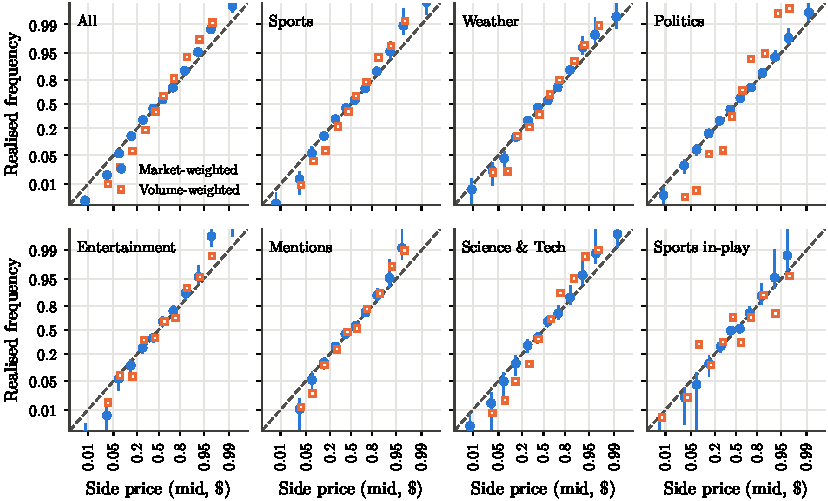
\includegraphics[width=\textwidth]{figures/fig_xs_calibration.pdf}
\caption{Calibration by group. Realised frequency of the side bought against its mid price, by
price bucket, on log-odds axes. Dots: market-weighted means with 95\% confidence intervals
clustered by event; open squares: volume-weighted (contracts traded in the 7 days to the quote).
Pre-event leads pooled; the last panel shows sports in-play quotes. The dashed line is perfect
calibration.}\label{fig:xs-calib}
\end{figure}

\begin{table}[!htbp]
\centering
\begin{threeparttable}
\caption{The favourite--longshot bias by group}\label{tab:xs-group}
\scriptsize
\setlength{\tabcolsep}{3pt}
\begin{tabular}{@{}lrrrrrrrrr@{}}
\toprule
% source: data/research/flb_xs/summary.json:measures_group
Group & Markets & Events & $\hat\beta$ & \LS & \FAV & \LS$-$\FAV & \LS & \FAV & \LS$-$\FAV \\
 & & & & \multicolumn{3}{c}{gross, at mid} & \multicolumn{3}{c}{net of taker fee, at ask} \\
\cmidrule(lr){5-7}\cmidrule(lr){8-10}
\midrule
\multicolumn{10}{@{}l}{\emph{A. Market-weighted}} \\
All groups & 19{,}007 & 4{,}770 & 1.129 & $-55.1$ & $+1.1$ & $-56.2$ & $-74.7$ & $-0.7$ & $-74.0$ \\
 &  &  & ($6.5$) & ($-10.0$) & ($9.8$) & ($-10.1$) & ($-25.3$) & ($-2.4$) & ($-24.1$) \\[2pt]
Sports & 6{,}284 & 1{,}521 & 1.099 & $-57.7$ & $+1.1$ & $-58.8$ & $-76.8$ & $-0.6$ & $-76.1$ \\
 &  &  & ($2.6$) & ($-4.3$) & ($4.8$) & ($-4.3$) & ($-11.0$) & ($-0.9$) & ($-10.6$) \\[2pt]
Weather & 2{,}901 & 1{,}065 & 1.152 & $-30.7$ & $+1.5$ & $-32.2$ & $-61.4$ & $-0.6$ & $-60.7$ \\
 &  &  & ($2.9$) & ($-1.4$) & ($4.0$) & ($-1.4$) & ($-5.2$) & ($-0.9$) & ($-5.0$) \\[2pt]
Politics & 3{,}906 & 968 & 1.075 & $-42.5$ & $+0.5$ & $-43.0$ & $-67.0$ & $-1.8$ & $-65.2$ \\
 &  &  & ($1.8$) & ($-4.5$) & ($2.2$) & ($-4.4$) & ($-12.2$) & ($-3.1$) & ($-11.3$) \\[2pt]
Entertainment & 2{,}665 & 530 & 1.254 & $-71.0$ & $+1.4$ & $-72.3$ & $-84.6$ & $-0.1$ & $-84.5$ \\
 &  &  & ($4.8$) & ($-8.2$) & ($6.9$) & ($-8.3$) & ($-18.7$) & ($-0.1$) & ($-17.6$) \\[2pt]
Mentions & 1{,}760 & 103 & 1.127 & $-75.8$ & $+1.6$ & $-77.4$ & $-85.0$ & $+0.5$ & $-85.5$ \\
 &  &  & ($2.0$) & ($-12.1$) & ($3.4$) & ($-11.6$) & ($-17.0$) & ($0.5$) & ($-15.3$) \\[2pt]
Science \& Tech & 1{,}375 & 510 & 1.175 & $-64.0$ & $+1.2$ & $-65.2$ & $-77.3$ & $-0.4$ & $-76.9$ \\
 &  &  & ($2.6$) & ($-6.0$) & ($3.7$) & ($-6.0$) & ($-11.0$) & ($-0.5$) & ($-10.1$) \\[2pt]
Other & 116 & 73 & 1.463 & $-95.2$ & $+2.9$ & $-98.1$ & $-95.7$ & $+3.2$ & $-98.9$ \\
 &  &  & ($2.4$) & ($-19.3$) & ($5.7$) & ($-18.2$) & ($-21.4$) & ($3.9$) & ($-19.0$) \\[2pt]
Sports in-play & 812 & 242 & 1.086 & $-74.1$ & $+1.4$ & $-75.5$ & $-82.3$ & $-0.1$ & $-82.2$ \\
 &  &  & ($1.1$) & ($-8.5$) & ($3.0$) & ($-8.3$) & ($-14.2$) & ($-0.1$) & ($-12.8$) \\[2pt]
\midrule
\multicolumn{10}{@{}l}{\emph{B. Volume-weighted (contracts traded in the 7 days to $t$)}} \\
All groups & 19{,}007 & 4{,}770 & 1.477 & $-85.6$ & $+1.6$ & $-87.3$ & $-90.5$ & $+1.8$ & $-92.3$ \\
 &  &  & ($3.6$) & ($-17.7$) & ($5.0$) & ($-17.6$) & ($-28.7$) & ($3.0$) & ($-25.8$) \\[2pt]
Sports & 6{,}284 & 1{,}521 & 1.373 & $-73.2$ & $+1.8$ & $-75.1$ & $-81.4$ & $+2.5$ & $-83.9$ \\
 &  &  & ($2.0$) & ($-5.6$) & ($3.2$) & ($-5.7$) & ($-9.7$) & ($1.9$) & ($-8.9$) \\[2pt]
Weather & 2{,}901 & 1{,}065 & 1.291 & $-81.0$ & $+1.3$ & $-82.3$ & $-87.2$ & $+2.1$ & $-89.3$ \\
 &  &  & ($2.0$) & ($-5.5$) & ($5.7$) & ($-5.5$) & ($-8.7$) & ($1.5$) & ($-7.9$) \\[2pt]
Politics & 3{,}906 & 968 & 1.795 & $-96.1$ & $+2.0$ & $-98.1$ & $-97.8$ & $+1.6$ & $-99.4$ \\
 &  &  & ($6.6$) & ($-67.0$) & ($2.6$) & ($-54.6$) & ($-120.7$) & ($6.0$) & ($-102.6$) \\[2pt]
Entertainment & 2{,}665 & 530 & 1.344 & $-85.3$ & $+0.9$ & $-86.2$ & $-90.7$ & $+0.3$ & $-91.0$ \\
 &  &  & ($3.0$) & ($-9.2$) & ($1.9$) & ($-8.9$) & ($-13.9$) & ($0.2$) & ($-11.7$) \\[2pt]
Mentions & 1{,}760 & 103 & 1.346 & $-92.0$ & $+1.4$ & $-93.4$ & $-93.6$ & $+2.1$ & $-95.7$ \\
 &  &  & ($4.6$) & ($-33.0$) & ($4.7$) & ($-31.6$) & ($-40.9$) & ($2.8$) & ($-33.3$) \\[2pt]
Science \& Tech & 1{,}375 & 510 & 1.564 & $-89.4$ & $+1.4$ & $-90.8$ & $-94.1$ & $+1.8$ & $-95.9$ \\
 &  &  & ($4.0$) & ($-22.4$) & ($6.8$) & ($-22.1$) & ($-39.5$) & ($3.4$) & ($-36.3$) \\[2pt]
Other & 116 & 73 & 1.431 & $-61.8$ & $+0.2$ & $-62.0$ & $-66.7$ & $+2.0$ & $-68.6$ \\
 &  &  & ($1.5$) & ($-1.5$) & ($0.1$) & ($-1.4$) & ($-1.9$) & ($0.5$) & ($-1.8$) \\[2pt]
Sports in-play & 812 & 242 & 0.810 & $+69.8$ & $-9.7$ & $+79.5$ & $+53.1$ & $-18.3$ & $+71.4$ \\
 &  &  & ($-0.6$) & ($0.5$) & ($-0.9$) & ($0.6$) & ($0.4$) & ($-1.2$) & ($0.5$) \\[2pt]
\bottomrule
\end{tabular}
\begin{tablenotes}\footnotesize
\item Pre-event quotes at leads of 1\,h to 30\,d before the scheduled time, pooled; sports in-play:
0.5--2\,h after the scheduled start. $\hat\beta$: slope of the logit regression~\eqref{eq:xs-logit},
with $t_{\beta=1}$ in parentheses. \LS, \FAV: mean return per dollar (\%) of sides priced at most
10\cents{} or at least 90\cents; \LS$-$\FAV: their difference. Gross: at the mid, no fee. Net: at the
ask, net of the exact taker fee, sides bucketed by the ask. Panel A gives each market weight one;
panel B weights quotes by contracts traded in the 7 days to the quote. $t$-statistics clustered
by event in parentheses.
\end{tablenotes}
\end{threeparttable}
\end{table}

\begin{figure}[!htbp]
\centering
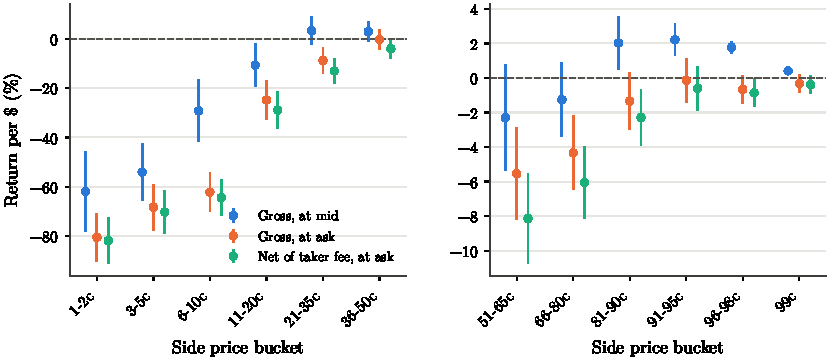
\includegraphics[width=\textwidth]{figures/fig_xs_returns.pdf}
\caption{Return per dollar by side-price bucket, all groups, market-weighted, pre-event leads
pooled: gross at the mid, gross at the ask, and net of the exact taker fee at the ask. Bars are
95\% confidence intervals clustered by event. The two panels share buckets but not the vertical
scale.}\label{fig:xs-returns}
\end{figure}

\begin{table}[!htbp]
\centering
\begin{threeparttable}
\caption{Calibration and returns by price bucket, all groups}\label{tab:xs-bucket}
\scriptsize
\begin{tabular}{@{}lrrrrrrr@{}}
\toprule
Bucket & Sides & Events & $\bar\q$ (\cents) & Win (\%) & Gross, mid (\%) & Gross, ask (\%) & Net, ask (\%) \\
\midrule
% source: data/research/flb_xs/tables/calibration.json:All.mkt
1-2c & 26{,}184 & 2{,}118 & 0.87 & 0.38 & $-62.0$ ($-7.5$) & $-80.6$ & $-81.8$ ($-17.3$) \\
3-5c & 9{,}521 & 2{,}007 & 3.53 & 1.67 & $-54.1$ ($-9.1$) & $-68.3$ & $-70.3$ ($-15.7$) \\
6-10c & 4{,}847 & 1{,}707 & 7.53 & 5.52 & $-29.2$ ($-4.5$) & $-62.2$ & $-64.4$ ($-17.1$) \\
11-20c & 6{,}366 & 1{,}919 & 15.18 & 13.73 & $-10.6$ ($-2.4$) & $-24.8$ & $-28.9$ ($-7.6$) \\
21-35c & 8{,}230 & 2{,}146 & 27.63 & 28.52 & $+3.4$ ($1.2$) & $-8.7$ & $-13.0$ ($-5.0$) \\
36-50c & 6{,}978 & 2{,}018 & 42.68 & 43.92 & $+3.0$ ($1.4$) & $-0.2$ & $-3.9$ ($-1.9$) \\
51-65c & 6{,}996 & 2{,}058 & 57.93 & 56.59 & $-2.3$ ($-1.5$) & $-5.5$ & $-8.1$ ($-6.2$) \\
66-80c & 8{,}254 & 2{,}150 & 72.95 & 72.02 & $-1.3$ ($-1.2$) & $-4.3$ & $-6.1$ ($-5.6$) \\
81-90c & 6{,}485 & 1{,}939 & 85.42 & 87.15 & $+2.0$ ($2.6$) & $-1.3$ & $-2.3$ ($-2.8$) \\
91-95c & 5{,}548 & 1{,}826 & 93.20 & 95.26 & $+2.2$ ($4.7$) & $-0.1$ & $-0.6$ ($-0.9$) \\
96-98c & 10{,}721 & 2{,}041 & 96.96 & 98.68 & $+1.8$ ($9.7$) & $-0.7$ & $-0.9$ ($-2.1$) \\
99c & 23{,}854 & 1{,}983 & 99.24 & 99.65 & $+0.4$ ($5.6$) & $-0.3$ & $-0.4$ ($-1.4$) \\
\bottomrule
\end{tabular}
\begin{tablenotes}\footnotesize
\item YES and NO sides of every usable pre-event quote, market-weighted. $\bar\q$: mean mid price of
the side; Win: weighted share that paid out. Returns per dollar; the ask columns bucket sides by
the ask. $t$-statistics clustered by event in parentheses.
\end{tablenotes}
\end{threeparttable}
\end{table}

\subsubsection{Horizon}\label{sec:res-xs-horizon}

Pooled across groups, the slope is $\xsTermAllThirtyDBeta$ at 30 days ($t=\xsTermAllThirtyDBetaT$),
$\xsTermAllSevenDBeta$ at 7 days, $\xsTermAllOneDBeta$ at 24 hours ($t=\xsTermAllOneDBetaT$) and
$\xsTermAllOneHBeta$ at one hour ($t=\xsTermAllOneHBetaT$) (\cref{tab:xs-term,fig:xs-term}). Prices
do not become calibrated as resolution approaches; if anything, the bias steepens in the last day.
The pattern is clearest in Entertainment, where the slope is $\xsTermEntThirtyDBeta$ at 30 days,
$\xsTermEntSevenDBeta$ at 7 days and $\xsTermEntOneDBeta$--$\xsTermEntSixHBeta$ within the last
day ($t=\xsTermEntOneDBetaT$ at 24 hours). Within other groups the cells are noisier and the
confidence intervals overlap across leads.

\citet{pageclemen2013} find calibration good at short horizons and a bias in long-dated contracts,
which they attribute to the cost of tying up capital. Kalshi's short horizons do not remove the bias.
This finding does not support a purely capital-cost explanation. The capital term of the no-arbitrage band
in \cref{sec:framework} scales with the horizon, so it predicts a bias that shrinks towards zero at short
leads. At one hour the opportunity cost of capital is negligible, yet the slope is at least as steep
as at 30 days.

\paragraph{Sports pre-game and in-play.}
For sports events with a scheduled start time in the ticker, the horizon is exact. Their pre-game
prices are close to calibrated: $\hat\beta=\xsTermSportsStartOneDBeta$ at 24 hours,
$\xsTermSportsStartSixHBeta$ at 6 hours and $\xsTermSportsStartOneHBeta$ one hour before the start
($t=\xsTermSportsStartOneHBetaT$). Half an hour into the game the slope is
$\xsTermSportsStartInHalfBeta$ ($t=\xsTermSportsStartInHalfBetaT$), and it is
$\xsTermSportsStartInOneBeta$ and $\xsTermSportsStartInTwoBeta$ one and two hours in. None of these
differs significantly from one. Longshots still lose in play: sides priced at most 10\cents{},
such as a team trailing late, return \xsInplayLsMid\% per dollar at the mid ($t=\xsInplayLsMidT$).
Most in-play longshot quotes sit in the 1--2\cents{} bucket, where the tick floor binds
(\cref{sec:res-xs-limits}).

\begin{figure}[!htbp]
\centering
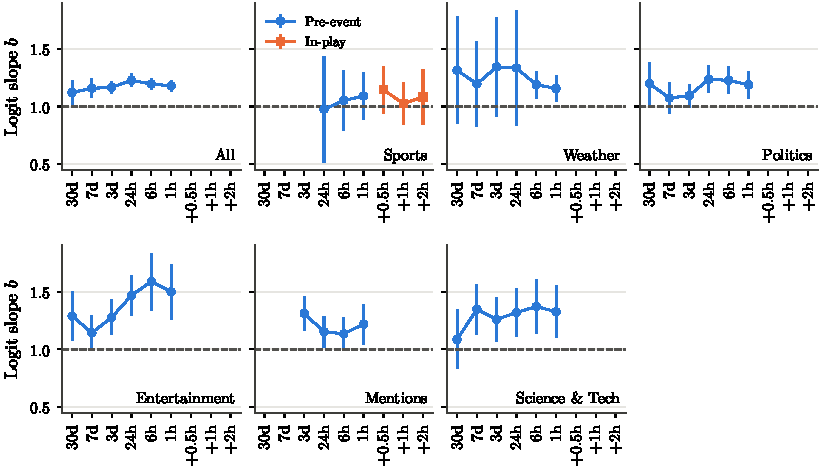
\includegraphics[width=\textwidth]{figures/fig_xs_term.pdf}
\caption{Term structure of the calibration slope $\hat\beta$ by group, from 30 days to 1 hour before
the scheduled time. The sports panel uses events with a start time in the ticker, before and 0.5, 1
and 2 hours after the start (in-play). One quote per market and lead; 95\% confidence intervals
clustered by event. The dashed line ($\beta=1$) is calibration.}\label{fig:xs-term}
\end{figure}

\begin{table}[!htbp]
\centering
\begin{threeparttable}
\caption{Calibration slope by lead and group}\label{tab:xs-term}
\scriptsize
\setlength{\tabcolsep}{3.5pt}
\begin{tabular}{@{}lrrrrrrr@{}}
\toprule
Lead & All & Sports & Weather & Politics & Entert. & Mentions & Sci.\,\&\,Tech \\
\midrule
% source: data/research/flb_xs/tables/term.json
1h & 1.180 & 1.092 & 1.158 & 1.190 & 1.501 & 1.218 & 1.326 \\
 & ($7.1$) & ($0.9$) & ($2.7$) & ($3.2$) & ($4.1$) & ($2.5$) & ($2.8$) \\[1pt]
6h & 1.196 & 1.053 & 1.190 & 1.228 & 1.590 & 1.135 & 1.372 \\
 & ($7.7$) & ($0.4$) & ($3.1$) & ($3.8$) & ($4.7$) & ($1.8$) & ($3.1$) \\[1pt]
24h & 1.229 & 0.976 & 1.335 & 1.238 & 1.469 & 1.151 & 1.320 \\
 & ($7.8$) & ($-0.1$) & ($1.3$) & ($3.9$) & ($5.3$) & ($2.2$) & ($2.9$) \\[1pt]
3d & 1.166 &  & 1.345 & 1.096 & 1.278 & 1.311 & 1.259 \\
 & ($5.9$) &  & ($1.6$) & ($1.9$) & ($3.6$) & ($4.1$) & ($2.7$) \\[1pt]
7d & 1.159 &  & 1.197 & 1.074 & 1.143 &  & 1.348 \\
 & ($3.8$) &  & ($1.0$) & ($1.1$) & ($1.8$) &  & ($3.1$) \\[1pt]
30d & 1.123 &  & 1.316 & 1.200 & 1.288 &  & 1.085 \\
 & ($2.3$) &  & ($1.3$) & ($2.1$) & ($2.6$) &  & ($0.6$) \\[1pt]
in-play 0.5h &  & 1.146 &  &  &  &  &  \\
 &  & ($1.4$) &  &  &  &  &  \\[1pt]
in-play 1h &  & 1.026 &  &  &  &  &  \\
 &  & ($0.3$) &  &  &  &  &  \\[1pt]
in-play 2h &  & 1.083 &  &  &  &  &  \\
 &  & ($0.7$) &  &  &  &  &  \\[1pt]
\bottomrule
\end{tabular}
\begin{tablenotes}\footnotesize
\item $\hat\beta$ of~\eqref{eq:xs-logit}, one quote per market and lead, market-weighted;
$t_{\beta=1}$ clustered by event in parentheses. The Sports column uses only events with a start
time in the ticker, so that the horizon is exact; in-play rows are 0.5, 1 and 2 hours after that
start. Cells with fewer than 100 quotes or 30 events are blank.
\end{tablenotes}
\end{threeparttable}
\end{table}

\subsubsection{Contract structure}\label{sec:res-xs-structure}

\Cref{tab:xs-structure,fig:xs-structure} compare the four contract structures. Multi-outcome
events and deadline contracts are the most biased; ladder legs and stand-alone binaries the least.

\paragraph{Deadline contracts.}
``By date'' contracts have $\hat\beta=\xsStDeadlineBeta$ ($t=\xsStDeadlineBetaT$), and their
longshots return \xsStDeadlineRegLsMid\% per dollar ($t=\xsStDeadlineRegLsMidT$). Only multi-outcome longshots lose more per dollar.

\paragraph{Ladder legs.}
Strike-ladder legs have $\hat\beta=\xsStLadderBeta$ ($t=\xsStLadderBetaT$). Their tails return
\xsStLadderRegLsMid\% per dollar at the mid ($t=\xsStLadderRegLsMidT$), and the body (35--65\cents)
\xsStLadderRegBodyMid\%. The implied distribution has tails that are too fat relative to outcomes,
the cross-strike form of the bias, but the tail loss is smaller than in the other structures.

\paragraph{Binaries.}
Stand-alone binaries have $\hat\beta=\xsStBinaryBeta$ ($t=\xsStBinaryBetaT$).

\paragraph{Multi-outcome events.}
Mutually exclusive events with at least three outcomes have $\hat\beta=\xsStMultiBeta$
($t=\xsStMultiBetaT$). \Cref{tab:xs-multi} shows where their mispricing sits.
\begin{itemize}
\item \emph{Overround.} Summed asks exceed one by \xsMeMultiOverAsk\% ($t=\xsMeMultiOverAskT$) in
      multi-outcome events and by \xsMeTwoOverAsk\% in two-leg events. That is the cost of buying the
      whole book, and it is mostly spread. In two-leg events the mids sum to one (\xsMeTwoOverMid\%).
      In multi-outcome events the mids themselves exceed one by \xsMeMultiOverMid\%
      ($t=\xsMeMultiOverMidT$): even at the mid, the book is overpriced.
\item \emph{Shin's insider share.} The median $\shinz$ is \xsMeMultiZMedian{} in multi-outcome and
      \xsMeTwoZMedian{} in two-leg events. These are of the same order as estimates for bookmaker
      markets \citep{shin1993}, but on an exchange $\shinz$ mostly restates the bid--ask spread.
      Median $\shinz$ is similar across groups (\cref{tab:xs-shin-group}).
\item \emph{The field.} Per event and lead, the legs priced at or below 10\cents{} cost
      \xsMeMultiFieldPrice\cents{} together and pay out \xsMeMultiFieldWin\cents{} on average: an
      overpricing of \xsMeMultiFieldGap\cents{} ($t=\xsMeMultiFieldGapT$). Realised minus price is
      \xsMeMultiRankOneEmid\cents{} for the favourite leg ($t=\xsMeMultiRankOneEmidT$) and
      \xsMeMultiRankSixEmid\cents{} for legs ranked sixth or lower ($t=\xsMeMultiRankSixEmidT$).
\end{itemize}
\Cref{fig:xs-multi} in the appendix plots these errors by rank.
Shin's adjustment moves probability from longshots to favourites, but with $\shinz$ near
\xsMeMultiZMedian{} the move is small. The field remains overpriced by \xsMeMultiFieldShinGap\cents{}
after the adjustment ($t=\xsMeMultiFieldShinGapT$), and the Brier score barely changes
(\xsMeMultiBrierMid{} raw, \xsMeMultiBrierShin{} Shin). The longshot overpricing in these events is
therefore not the price protection against insiders that Shin's model implies. It is closer to many
small bets spread over the field. Within multi-outcome events the slope does not rise with the number
of outcomes: it is $\xsMultiLegsThreeBeta$ for 3--5 legs, $\xsMultiLegsSixBeta$ for 6--10,
$\xsMultiLegsElevenBeta$ for 11--20 and $\xsMultiLegsTwentyOneBeta$ for more.

\begin{table}[!htbp]
\centering
\begin{threeparttable}
\caption{The bias by contract structure}\label{tab:xs-structure}
\scriptsize
\setlength{\tabcolsep}{3.5pt}
\begin{tabular}{@{}lrrrrrrrr@{}}
\toprule
 & & & & \multicolumn{3}{c}{Gross, at mid} & \multicolumn{2}{c}{Net, at ask} \\
\cmidrule(lr){5-7}\cmidrule(l){8-9}
Structure & Markets & Events & $\hat\beta$ & \LS & 35--65\cents & \FAV & \LS & \FAV \\
\midrule
% source: data/research/flb_xs/tables/structure.json
Binary & 6{,}028 & 2{,}644 & 1.120 & $-64.1$ & $+0.2$ & $+1.7$ & $-79.0$ & $-0.0$ \\
 &  &  & ($3.7$) & ($-9.0$) & ($0.4$) & ($6.4$) & ($-17.8$) & ($-0.0$) \\[2pt]
Multi-outcome & 3{,}441 & 474 & 1.283 & $-71.8$ & $+0.6$ & $+1.1$ & $-84.4$ & $+0.4$ \\
 &  &  & ($4.4$) & ($-8.3$) & ($0.6$) & ($7.2$) & ($-18.1$) & ($0.6$) \\[2pt]
Ladder leg & 7{,}029 & 1{,}030 & 1.118 & $-30.9$ & $+0.4$ & $+0.9$ & $-61.6$ & $-1.4$ \\
 &  &  & ($2.9$) & ($-2.3$) & ($0.9$) & ($3.9$) & ($-8.8$) & ($-2.9$) \\[2pt]
Deadline & 2{,}509 & 644 & 1.224 & $-68.3$ & $+3.3$ & $+0.9$ & $-81.1$ & $-1.1$ \\
 &  &  & ($3.9$) & ($-10.7$) & ($2.4$) & ($4.0$) & ($-20.0$) & ($-1.4$) \\[2pt]
\bottomrule
\end{tabular}
\begin{tablenotes}\footnotesize
\item Structures as defined in \cref{sec:method-xs}. Returns per dollar (\%) of sides in three price
regions; market-weighted; pre-event leads pooled; $t$-statistics clustered by event in parentheses
($t_{\beta=1}$ under $\hat\beta$).
\end{tablenotes}
\end{threeparttable}
\end{table}

\begin{figure}[!htbp]
\centering
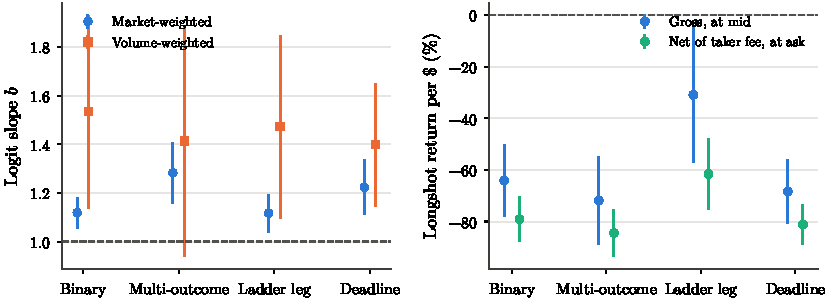
\includegraphics[width=\textwidth]{figures/fig_xs_structure.pdf}
\caption{Contract structure. Left: calibration slope, market- and volume-weighted. Right: return per
dollar on longshot sides ($\q\le10\cents$), gross at the mid and net of the taker fee at the ask.
95\% confidence intervals clustered by event.}\label{fig:xs-structure}
\end{figure}

\begin{table}[!htbp]
\centering
\begin{threeparttable}
\caption{Mutually exclusive events: overround, Shin $\shinz$ and where the mispricing sits}\label{tab:xs-multi}
\scriptsize
\setlength{\tabcolsep}{3.5pt}
\begin{tabular}{@{}lrrrrrrrr@{}}
\toprule
 & Events & Event-leads & Legs & $\sum a-1$ (\%) & $\sum p-1$ (\%) & $\sum b-1$ (\%) & Mean $\shinz$ & Median $\shinz$ \\
\midrule
% source: data/research/flb_xs/tables/structure.json:multi_outcome
Two-leg events & 740 & 2{,}009 & 2 & $+2.8$ ($41.3$) & $-0.1$ ($-3.2$) & $-3.0$ & 0.030 & 0.020 \\
Multi-outcome events ($\geq 3$ legs) & 381 & 1{,}289 & 4 & $+9.7$ ($16.6$) & $+2.3$ ($7.8$) & $-5.2$ & 0.025 & 0.017 \\
\bottomrule
\end{tabular}

\vspace{6pt}
\begin{tabular}{@{}lrrrrrr@{}}
\toprule
Leg rank & Legs & Mid (\cents) & Win (\%) & Win $-$ mid (\cents) & Win $-$ normalised (\cents) & Win $-$ Shin (\cents) \\
\midrule
% source: data/research/flb_xs/tables/structure.json:multi_outcome.multi (by_rank, field)
1 (favourite) & 1{,}289 & 68.4 & 69.8 & $+1.46$ ($0.8$) & $+3.08$ ($1.6$) & $+3.33$ ($1.7$) \\
2 & 1{,}289 & 18.2 & 16.4 & $-1.80$ ($-1.1$) & $-1.55$ ($-0.9$) & $-1.65$ ($-1.0$) \\
3-5 & 2{,}565 & 6.8 & 6.5 & $-0.33$ ($-0.4$) & $-0.24$ ($-0.3$) & $-0.34$ ($-0.4$) \\
6+ & 2{,}933 & 0.9 & 0.4 & $-0.55$ ($-3.8$) & $-0.47$ ($-3.3$) & $-0.44$ ($-3.1$) \\
\midrule
Field ($\leq 10\cents$ legs) & 762 & 9.7 & 5.4 & $-4.34$ ($-3.4$) & $-3.77$ ($-3.0$) & $-3.97$ ($-3.2$) \\
\bottomrule
\end{tabular}
\begin{tablenotes}\footnotesize
\item Top: events flagged mutually exclusive by Kalshi with every leg quoted at the lead and
exactly one leg settling YES; one observation per event and lead. $a$, $p$, $b$: YES ask, mid and
bid; $\shinz$ from the asks via~\eqref{eq:xs-shin}. Bottom: legs of events with at least three
legs, ranked by mid within the event and lead. Normalised: mid divided by the event's sum of mids.
Shin: $\hat p_k(\shinz)$. Field: per event and lead, all legs priced at or below 10\cents{} together
(their summed price against the number that win). $t$-statistics clustered by event in parentheses.
\end{tablenotes}
\end{threeparttable}
\end{table}

\subsubsection{Liquidity and calendar time}\label{sec:res-xs-liquidity}

\paragraph{Liquidity.}
The bias is not confined to thin markets (\cref{fig:xs-liq}, \cref{tab:xs-liq}). Across
within-group terciles of trailing 7-day volume, the slope is $\xsLiqVolLowBeta$, $\xsLiqVolMidBeta$
and $\xsLiqVolHighBeta$ ($t=\xsLiqVolHighBetaT$ in the top tercile). Across open-interest terciles it
is $\xsLiqOiLowBeta$, $\xsLiqOiMidBeta$ and $\xsLiqOiHighBeta$, and across spread terciles
$\xsLiqSpreadLowBeta$ (tightest), $\xsLiqSpreadMidBeta$ and $\xsLiqSpreadHighBeta$ (widest). Longshot
returns at the mid are, if anything, more negative in the most active tercile: \xsLiqVolHighLsMid\%,
against \xsLiqVolLowLsMid\% in the least active. Volume-weighted estimates are steeper than all
terciles (\cref{sec:res-xs-size}). The very largest markets, which dominate volume-weighted averages
but are a small part of the top tercile, are the most biased.

\paragraph{Calendar time.}
The slope is above one in \xsCalBetaAboveOne{} of the \xsCalNQtr{} quarters from \xsCalFirstQtr{} to
\xsCalLastQtr{} (\cref{fig:xs-liq,tab:xs-cal}).
\begin{itemize}
\item Before 2025 the venue was small (about \xsVenueEarlyMkts{} in-scope markets a quarter in 2022),
      and the quarterly slopes are noisy, ranging from $\xsCalEarlyMin$ to $\xsCalEarlyMax$.
\item From 2025, as sports listings took the venue to \xsVenuePeakMkts{} settled markets in
      \xsVenuePeakQtr, the slope settles between $\xsCalRecentMin$ and $\xsCalRecentMax$ in all
      \xsCalRecentN{} quarters.
\end{itemize}
Growth by three orders of magnitude neither removed the bias nor visibly reduced it. Whatever capital entered on the other side was not enough to remove it.

\begin{figure}[!htbp]
\centering
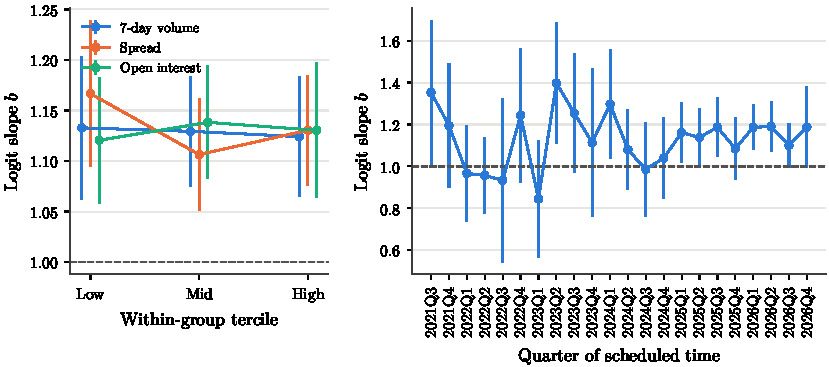
\includegraphics[width=\textwidth]{figures/fig_xs_liq_calendar.pdf}
\caption{Left: calibration slope by within-group tercile of 7-day volume, quoted spread and open
interest at the quote. Right: calibration slope by quarter of the scheduled time, all groups. Both
market-weighted, pre-event leads pooled; 95\% confidence intervals clustered by event.}\label{fig:xs-liq}
\end{figure}

\subsubsection{Fees, the tick and the limits to arbitrage}\label{sec:res-xs-limits}

\paragraph{Fees.}
Kalshi's taker fee is $0.07\,\q(1-\q)$ per contract, or $7(1-\q)$\% per dollar staked, so it is
almost flat per dollar for longshots (\cref{fig:xs-limits}, left). Kalshi computes the fee per fill to
\$0.000001 and rebates rounding over-payment \citep{kalshirounding}, so the exact fee is the fee
paid. Under a rule that rounded each order up to the cent, a single 1\cents{} contract would pay a
1\cents{} fee, 100\% of the stake; the figure shows this case for comparison. Net of fees and the half-spread, longshot
returns fall from \xsAllLsMid\% to \xsAllLsNet\% (\cref{tab:xs-group}). Fees and spread thus deepen the
longshot buyer's loss without changing its sign.

\paragraph{Taking the other side.}
The arbitrageur's question is whether buying the favourite side of every longshot pays
(\cref{tab:xs-limits}, bottom). At the mid it returns \xsOtherAllMid\% per dollar ($t=\xsOtherAllMidT$).
As a taker at the ask, net of fees, it returns \xsOtherAllTakerNet\% ($t=\xsOtherAllTakerNetT$): the
spread and fee absorb the whole premium. Resting at the bid as a maker would return \xsOtherAllMakerNet\%
($t=\xsOtherAllMakerNetT$) if every order filled at the quote. That is an upper bound: fills on resting
orders are adversely selected (\cref{sec:res-flow}).

\paragraph{The no-arbitrage band.}
\Cref{fig:xs-limits} (right) sets the mispricing per contract against the cost of trading against it.
\begin{itemize}
\item In the longshot buckets, price minus realised frequency is \xsBandBOneMis, \xsBandBThreeMis{}
      and \xsBandBSixMis{} cents per contract for 1--2, 3--5 and 6--10\cents.
\item The taker's cost (half-spread plus fee on the opposite side) is \xsBandBOneCost,
      \xsBandBThreeCost{} and \xsBandBSixCost{} cents.
\item The mispricing lies inside the taker band in \xsBandInside{} of \xsBandN{} buckets; in the three
      longshot buckets it takes up \xsBandShareMin--\xsBandShareMax\% of the band.
\end{itemize}
The longshot overpricing thus sits close to the edge of the band: most of the cost of removing it,
and no more. This is the classic limit to arbitrage \citep{shleifervishny1997}, here
created by the spread and the fee schedule rather than by capital constraints. The capital term of
the band in \cref{sec:framework} adds little at these horizons: at a 5\%
annual cost of capital, holding a 95\cents{} favourite for 30 days costs about 0.4\cents{} per
contract, and for one day about 0.01\cents.

\paragraph{The tick floor.}
The floor binds often.
\begin{itemize}
\item \xsFloorShareEither\% of quotes have a side priced at or below 2\cents, and \xsFloorSharePinned\%
      sit at the floor with no bid and a 1\cents{} ask.
\item Sides pinned there win \xsFloorPinnedWin\% of the time against a 0.5\cents{} mid. A contract worth
      about a tenth of a cent cannot be quoted lower.
\item Splitting the 1--2\cents{} bucket's loss of \xsFloorAllLoss{} cents per contract,
      \xsFloorAllMechShare\% is mechanical, the loss of quotes at the floor.
\item For a taker paying a 1--2\cents{} ask, the mechanical share is \xsFloorTakerMechShare\%: the
      1\cents{} ask alone costs nearly a cent against a win rate of \xsFloorTakerWin\%.
\end{itemize}
The rest of the 1--2\cents{} loss comes from prices above the floor. Only \xsSubcentShare\% of
markets quote on a 0.1\cents{} grid, too few for a clean comparison.

\begin{figure}[!htbp]
\centering
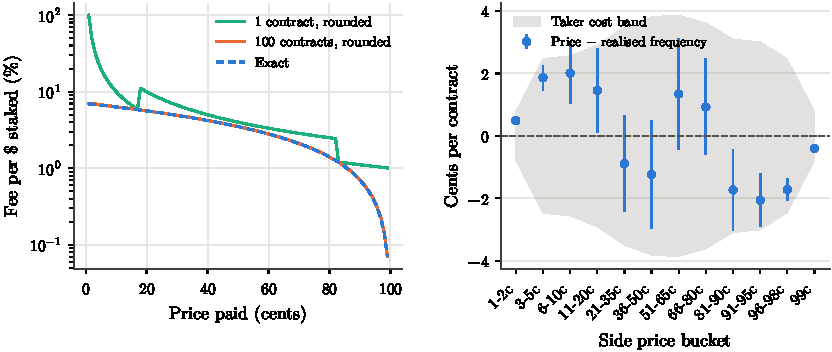
\includegraphics[width=\textwidth]{figures/fig_xs_limits.pdf}
\caption{Limits to arbitrage. Left: Kalshi taker fee per dollar staked against the price paid,
exact and rounded up to the cent for one order of 1 or 100 contracts (log scale). Right: mispricing
per contract at the mid (side price minus realised frequency, with 95\% confidence intervals
clustered by event) against the cost of trading against it as a taker (half-spread plus the taker
fee on the opposite side, shaded), by bucket of the side price.}\label{fig:xs-limits}
\end{figure}

\begin{table}[!htbp]
\centering
\begin{threeparttable}
\caption{The tick floor and the other side of longshots}\label{tab:xs-limits}
\scriptsize
\setlength{\tabcolsep}{3.5pt}
\begin{tabular}{@{}lrrrrrrr@{}}
\toprule
 & Sides & Price (\cents) & Win (\%) & Loss (\cents) & Mechanical (\cents) & Share & Return (\%) \\
\midrule
% source: data/research/flb_xs/tables/limits.json:floor
All 1--2\cents{} sides (1\cents{} grid) & 25{,}800 & 0.87 & 0.38 & 0.49 & 0.22 & 45\% & $-61.6$ ($-7.4$) \\
\quad at the floor (mid 0.5\cents) & 15{,}747 & 0.50 & 0.13 & 0.37 & 0.37 & 100\% & $-73.5$ ($-7.5$) \\
\quad above the floor & 10{,}053 & 1.44 & 0.77 & 0.67 & 0.00 & 0\% & $-43.3$ ($-3.7$) \\
0--2\cents{} sides, 0.1\cents{} grid & 384 & 0.75 & 0.00 & 0.75 & 0.01 & 1\% & $-100.0$  \\
Taker at a 1--2\cents{} ask & 20{,}948 & 1.25 & 0.29 & 0.95 & 0.65 & 68\% & $-81.6$ ($-17.1$) \\
\bottomrule
\end{tabular}

\vspace{6pt}
\begin{tabular}{@{}lrrrrr@{}}
\toprule
Buying the favourite side & Sides & Gross, mid (\%) & Gross, ask (\%) & Taker net (\%) & Maker net (\%) \\
\midrule
% source: data/research/flb_xs/tables/limits.json:other_side
All groups & 40{,}552 & $+1.11$ ($9.8$) & $-0.27$ ($-0.9$) & $-0.49$ ($-1.7$) & $+2.64$ ($21.3$) \\
Sports & 9{,}108 & $+1.11$ ($4.8$) & $+0.06$ ($0.1$) & $-0.17$ ($-0.2$) & $+2.58$ ($9.8$) \\
Weather & 3{,}905 & $+1.51$ ($4.0$) & $+0.05$ ($0.1$) & $-0.19$ ($-0.3$) & $+3.41$ ($8.6$) \\
Politics & 11{,}768 & $+0.52$ ($2.2$) & $-1.38$ ($-2.5$) & $-1.59$ ($-2.9$) & $+1.95$ ($7.8$) \\
Entertainment & 8{,}939 & $+1.36$ ($6.9$) & $+0.16$ ($0.2$) & $-0.06$ ($-0.1$) & $+2.97$ ($13.1$) \\
Mentions & 1{,}918 & $+1.63$ ($3.4$) & $+0.77$ ($0.9$) & $+0.49$ ($0.6$) & $+2.92$ ($5.5$) \\
Science \& Tech & 4{,}572 & $+1.16$ ($3.7$) & $-0.20$ ($-0.3$) & $-0.40$ ($-0.5$) & $+2.57$ ($7.3$) \\
Other & 342 & $+2.85$ ($5.7$) & $+2.66$ ($2.9$) & $+2.42$ ($2.6$) & $+4.40$ ($8.1$) \\
\bottomrule
\end{tabular}
\begin{tablenotes}\footnotesize
\item Top: sides priced at most 2\cents. Loss: price minus realised win rate, per contract.
Mechanical: the loss of sides quoted at the floor (mid 0.5\cents{} with no bid, or a 1\cents{} ask
for takers), $\max(\text{floor}-\text{win},0)$, times their weight share. Return: gross per dollar at
the mid, or net at the ask for the taker row. Bottom: buying the favourite side ($\q\ge 90\cents$ at
the mid) of every quote: at the mid; at the ask as a taker, gross and net of the taker fee; and
resting at the bid as a maker, net of the maker fee where the series charges one. The maker column
assumes a fill at the quote and ignores adverse selection, so it is an upper bound. Market-weighted;
$t$-statistics clustered by event in parentheses.
\end{tablenotes}
\end{threeparttable}
\end{table}

\subsubsection{Robustness}\label{sec:res-xs-robust}

The appendix collects the robustness checks (\cref{tab:xs-robust,tab:xs-cluster}).
\begin{itemize}
\item \emph{Sample halves.} Splitting at the median observation date (\xsRobSplit) gives
      $\hat\beta=\xsRobFirstBeta$ ($t=\xsRobFirstBetaT$) and $\xsRobSecondBeta$ ($t=\xsRobSecondBetaT$),
      and longshot returns of \xsRobFirstLsMid\% and \xsRobSecondLsMid\%. The slope exceeds one in
      \xsRobFirstGroupsAboveOne{} of \xsRobFirstGroups{} groups in the first half and
      \xsRobSecondGroupsAboveOne{} of \xsRobSecondGroups{} in the second.
\item \emph{Without the tick-floor buckets.} Dropping quotes with a mid at or below 2\cents{} or at or
      above 98\cents{} leaves $\hat\beta=\xsRobInnerBeta$ ($t=\xsRobInnerBetaT$). The slope is
      therefore not an artefact of the floor.
\item \emph{Other filters and weights.} Restricting to spreads of at most 5\cents{}
      ($\hat\beta=\xsRobSpreadBeta$) or quotes at most a day old ($\xsRobFreshBeta$), or reweighting
      by the inverse sampling probability ($\xsRobDesignBeta$, $t=\xsRobDesignBetaT$), changes little.
\item \emph{Clustering.} The test of $\beta=1$ has $t=\xsCluMarketBetaT$ when clustered by market,
      $\xsCluSeriesBetaT$ by series and $\xsCluMonthBetaT$ by calendar month.
\end{itemize}

\subsubsection{Mechanical and behavioural components}\label{sec:res-xs-summary}

The measures above separate the components that \cref{sec:framework} distinguishes.
\begin{itemize}
\item \emph{Mechanical.} The tick floor explains about half of the loss in the cheapest bucket
      (\xsFloorAllMechShare\% at the mid, \xsFloorTakerMechShare\% for a taker at the ask). Fees and
      spreads deepen buyers' losses and make the remaining mispricing uneconomic to trade against:
      the longshot overpricing lies inside the taker band, close to its edge. In this sense the bias
      survives fees for the buyer and does not survive them for the arbitrageur.
\item \emph{Not only mechanical.} The slope is $\xsRobInnerBeta$ without the floor buckets. It does
      not shrink at short horizons, where capital costs vanish. It is as strong where volume and open
      interest are high as where they are low, and it is present in every group and in both halves of
      the sample. Mechanics set the band; something else keeps prices near its edge.
\item \emph{Not insiders.} In multi-outcome events, Shin's $\shinz$ is about \xsMeMultiZMedian{} and
      largely a restatement of the spread, and the Shin adjustment leaves the field overpriced. This
      is contrary to the information hypothesis of \cref{sec:framework}.
\item \emph{Consistent with demand for lottery-like payoffs.} The bias is steepest in multi-outcome
      fields, in deadline contracts and in entertainment, where outcomes have no external anchor. It
      is weakest in politics and in pre-game sports with a known start, where polls and bookmaker
      lines provide one. This pattern is consistent with the preference and belief-dispersion
      explanations of \cref{sec:framework}, although the cross-group differences are modest. \Cref{sec:res-flow,sec:res-wallets} ask who is on each side of
      these trades.
\end{itemize}

\subsection{Who pays: takers, trade size and timing}\label{sec:res-flow}
% source: data/research/flb_flow/summary.json (coverage, strata, sign_tests), tables/*.csv
This subsection uses the main trade sample: 2,685,117 pre-resolution prints in 14,164 markets and
2,151 events. They make up 1,643,534 taker orders, 277 million contracts and \$132 million of
taker notional (\cref{tab:flow-coverage}). Two features of the data shape how we report the
results.
\begin{itemize}
  \item \emph{Pooled means are dominated by sports and by a few upsets.} Sports carry 98.6\% of
  the frame's volume, so design-weighted pooled means are close to sports means. Longshot payoffs
  are also extremely right-skewed. In the pooled taker longshot estimate, a single MLB home-run
  prop event contributes 40\% of the design-weighted profit, and one Challenger tennis match
  another 29\%. Pooled per-dollar returns on longshots are therefore imprecise. They can even
  change sign when one event is added or removed.
  \item \emph{Each stratum is a self-weighting random sample.} We therefore rely on statistics
  that are robust to this: each stratum's own estimate, a sign test across the 18 independent
  strata, and the median stratum in the figures. We also rely on quantities that are not
  heavy-tailed, namely who trades at which price, spreads and fees.
\end{itemize}
Pooled estimates with event-clustered $t$-statistics are reported throughout as well.

\subsubsection{Takers against makers}\label{sec:res-flow-roles}

% source: data/research/flb_flow/tables/roles_overall.csv, roles_diff.csv, strata.csv, roles_bucket_strata.csv; summary.json (sign_tests)
\paragraph{Across all prices, liquidity role does not decide who loses.} Pooled over every
print, takers earn $-2.4\%$ per dollar after fees ($t=-0.7$) and makers $-0.4\%$ ($t=-0.1$). The
difference is $-2.0$ percentage points ($t=-0.3$; \cref{tab:flow-roles}). Takers do worse than
makers in only 9 of the 18 strata. Some groups show clear role differences, but they point both
ways:
\begin{itemize}
  \item in Mentions, takers lose 5.1\% ($t=-2.3$) while makers earn 1.6\%;
  \item in Weather, takers lose 3.0\% ($t=-2.4$);
  \item in Science \& Tech the sign reverses: takers earn 4.5\% ($t=5.8$) and makers lose 7.9\%
  ($t=-6.5$).
\end{itemize}
So the maker advantage that \citet{burgi2025} document on average is not uniform across
categories.

\paragraph{At the longshot end, both roles lose, and takers lose more.} \Cref{fig:flow-roles}
and \cref{tab:flow-strata} show the per-stratum results.
\begin{itemize}
  \item In the median stratum, takers who buy at 1--2\cents{} lose 89\% of the stake. At
  3--5\cents{} they lose 69\%, and at 6--10\cents{} 52\%.
  \item Makers who hold sides at the same prices lose 48\%, 27\% and 27\%.
  \item Taker longshot positions lose in 14 of 18 strata (one-sided sign test $p=0.015$). Maker
  longshot positions lose in 12 of 18 ($p=0.12$). Takers do worse than makers on longshots in 13
  of 18 ($p=0.048$).
  \item The losses are large and precisely estimated in politics ($-57\%$, $t=-3.0$),
  entertainment ($-28\%$, $t=-3.1$), mentions ($-63\%$, $t=-5.6$) and most sports leagues. In
  NBA, NCAAF, NHL and the other-sports stratum they reach $-84$ to $-97\%$, with $|t|>8$.
  \item The four exceptions are MLB, golf, tennis and Science \& Tech. Each is driven by one or
  two events in which a heavily traded longshot won. Without its two most profitable events,
  the stratum's taker longshot return falls to $-64\%$ in golf and $-85\%$ in tennis, and to
  $+22\%$ in MLB and $+12\%$ in Science \& Tech.
  \item Favourites earn roughly zero for both roles: between $-1\%$ and $+3\%$ per dollar in the
  median stratum at $\q\ge81\cents$.
\end{itemize}
This is the pattern of \citet{burgi2025}: the bias is present for both roles and stronger for
takers. \Cref{tab:flow-buckets} gives the pooled estimates by bucket, and
\cref{fig:flow-roles-groups} gives them by group.

\paragraph{Takers are the majority buyers of longshots.} Takers hold 56--64\% of the contracts
bought at $\q\le20\cents$, but only 39--44\% of those bought at $\q\ge81\cents$
(\cref{fig:flow-roles}b). The typical longshot print is therefore a taker buying the longshot
from a resting order that sells it, and the maker ends up holding the favourite.

\paragraph{Why takers lose more: the price of immediacy.} \Cref{tab:flow-decomp} splits the
taker's gross profit into the mispricing of the mid-quote and the effective half-spread.
\begin{itemize}
  \item On longshots (mean price 5.5\cents) the taker pays a half-spread of 0.51\cents{} per
  contract ($t=14.4$) and a fee of 0.33\cents.
  \item Together this is 14\% of the stake: 14\% in sports and 21\% in non-sports.
  \item The same cost is 4\% for mid-priced contracts and 1.5\% for favourites.
\end{itemize}
The immediacy cost is precisely measured, and it falls on the taker alone. The remaining term,
the gap between the outcome and the mid-quote, is the bias in the price itself. Takers and makers
share it, and trade by trade it is too noisy to pin down in the pooled sample ($+2.4\cents$,
$t=0.8$). \Cref{sec:res-xs} measures it from prices. Because the immediacy cost is a fixed
amount per contract, it is largest per dollar on the cheapest contracts. Takers pay it there,
which is exactly what a favourite--longshot pattern in taker returns requires.

\begin{figure}[htbp]
\centering
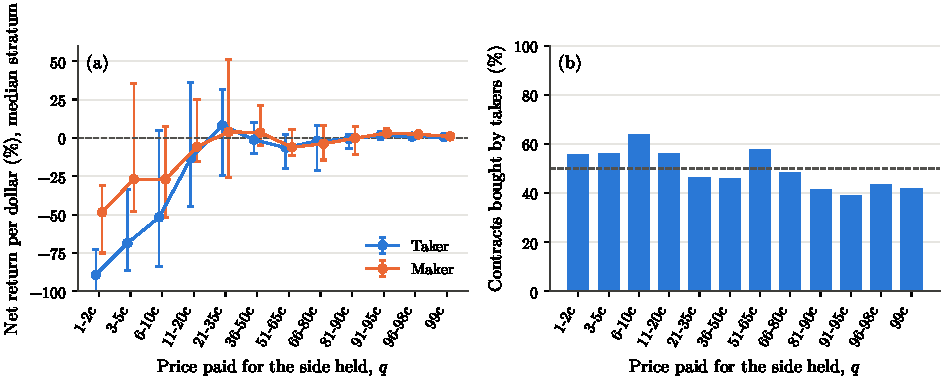
\includegraphics[width=\textwidth]{figures/fig_flow_roles.pdf}
\caption{Takers against makers by the price of the side held. (a) Net return per dollar
(dollar-weighted, after each role's fee) of taker and maker positions: the median across the 18
strata of each stratum's estimate, with bars spanning the interquartile range across strata
(strata with at least five events in the cell). (b) Takers' share of the contracts held at each
price, pooled and design-weighted. Main sample.}\label{fig:flow-roles}
% source: data/research/flb_flow/tables/roles_bucket.csv, roles_bucket_strata.csv
\end{figure}

\begin{table}[htbp]
\centering
\begin{threeparttable}
\caption{Net return per dollar of takers and makers, by group}\label{tab:flow-roles}
\footnotesize
\setlength{\tabcolsep}{4pt}
\begin{tabular}{@{}lrrrrrrr@{}}
\toprule
 & \multicolumn{3}{c}{All positions} & \multicolumn{3}{c}{Longshot positions ($\q\le10\cents$)} & \\
\cmidrule(lr){2-4}\cmidrule(lr){5-7}
Group & Taker & Maker & Difference & Taker & Maker & Taker share & Events \\
\midrule
% source: data/research/flb_flow/tables/roles_overall.csv, roles_diff.csv, roles_side.csv
%BEGIN:roles_group
% source: data/research/flb_flow (generated by flb_flow tex)
Sports & $-2.4$ $(-0.7)$ & $-0.4$ $(-0.1)$ & $-2.0$ $(-0.3)$ & $+52.0$ $(1.0)$ & $+49.9$ $(0.8)$ & $59$ & 1,003 \\
Weather & $-3.0$ $(-2.4)$ & $+1.2$ $(1.3)$ & $-4.2$ $(-1.9)$ & $-15.7$ $(-0.3)$ & $+85.4$ $(0.7)$ & $61$ & 297 \\
Politics & $+1.1$ $(0.6)$ & $-2.1$ $(-1.2)$ & $+3.2$ $(0.9)$ & $-57.2$ $(-3.0)$ & $-37.9$ $(-2.2)$ & $61$ & 258 \\
Entertainment & $+0.3$ $(0.5)$ & $-1.3$ $(-2.3)$ & $+1.6$ $(1.4)$ & $-27.9$ $(-3.1)$ & $-28.4$ $(-2.4)$ & $56$ & 258 \\
Mentions & $-5.1$ $(-2.3)$ & $+1.6$ $(1.7)$ & $-6.8$ $(-2.1)$ & $-62.9$ $(-5.6)$ & $-36.9$ $(-2.2)$ & $76$ & 119 \\
Science \& Tech & $+4.5$ $(5.8)$ & $-7.9$ $(-6.5)$ & $+12.4$ $(6.5)$ & $+92.1$ $(1.5)$ & $-8.2$ $(-0.2)$ & $36$ & 216 \\
\midrule
Non-sports & $-0.9$ $(-1.0)$ & $-0.4$ $(-0.5)$ & $-0.5$ $(-0.3)$ & $-31.0$ $(-1.5)$ & $+11.9$ $(0.3)$ & $60$ & 1,148 \\
All & $-2.4$ $(-0.7)$ & $-0.4$ $(-0.1)$ & $-2.0$ $(-0.3)$ & $+48.9$ $(1.0)$ & $+48.4$ $(0.8)$ & $59$ & 2,151 \\
%END:roles_group
\bottomrule
\end{tabular}
\begin{tablenotes}\footnotesize
\item Main sample, design-weighted. Net return per dollar is dollar-weighted
\eqref{eq:flow-d} after each role's fee, in percent. $t$-statistics clustered by event are in
parentheses. Difference: taker minus maker on the same prints, in percentage points.
Longshot positions are positions in a side bought at $\q\le10\cents$: the taker's side when the
taker bought the longshot, and the maker's side when the taker bought the favourite. Taker share:
the takers' share of longshot contracts held. All pools the groups with design weights and is
dominated by sports.
\end{tablenotes}
\end{threeparttable}
\end{table}

\begin{table}[htbp]
\centering
\begin{threeparttable}
\caption{Longshot positions by stratum: returns, buyers and spreads}\label{tab:flow-strata}
\footnotesize
\setlength{\tabcolsep}{3pt}
\begin{tabular}{@{}lrrrrrrr@{}}
\toprule
 & & \multicolumn{3}{c}{Longshot return (\%/\$)} & \multicolumn{2}{c}{Share at $\q\le10\cents$ (\%)} & Half- \\
\cmidrule(lr){3-5}\cmidrule(lr){6-7}
 & & & & Orders & Orders & Orders & spread \\
Stratum & Events & Takers & Makers & $\le\$100$ & $\le\$10$ & $>\$1$k & (\cents) \\
\midrule
% source: data/research/flb_flow/tables/strata.csv, summary.json (sign_tests)
%BEGIN:strata
% source: data/research/flb_flow (generated by flb_flow tex)
Combat & 59 & $-65$ $(-2.4)$ & $-75$ $(-3.1)$ & $-63$ $(-2.1)$ & $26$ & $0.2$ & $+0.42$ \\
Cricket & 60 & $-57$ $(-1.8)$ & $-36$ $(-0.9)$ & $-59$ $(-2.3)$ & $66$ & $0.8$ & $+0.55$ \\
Esports & 85 & $-86$ $(-8.0)$ & $+37$ $(0.4)$ & $-80$ $(-5.7)$ & $24$ & $0.0$ & $+0.96$ \\
Golf & 30 & $+141$ $(2.1)$ & $+73$ $(1.9)$ & $+218$ $(2.3)$ & $87$ & $36.2$ & $+0.47$ \\
MLB & 87 & $+223$ $(3.9)$ & $+96$ $(1.0)$ & $+191$ $(3.5)$ & $55$ & $2.1$ & $+0.61$ \\
NBA & 49 & $-97$ $(-46.0)$ & $-70$ $(-4.4)$ & $-95$ $(-31.5)$ & $43$ & $0.0$ & $+0.67$ \\
NCAAF & 78 & $-86$ $(-11.6)$ & $-35$ $(-1.1)$ & $-78$ $(-7.0)$ & $38$ & $0.0$ & $+0.29$ \\
NFL & 60 & $-49$ $(-1.5)$ & $+28$ $(0.8)$ & $-63$ $(-3.1)$ & $14$ & $1.0$ & $+0.48$ \\
NHL & 60 & $-84$ $(-8.7)$ & $-59$ $(-1.8)$ & $-80$ $(-6.6)$ & $54$ & $0.0$ & $+0.40$ \\
Other sports & 123 & $-87$ $(-11.4)$ & $-73$ $(-5.7)$ & $-86$ $(-10.3)$ & $77$ & $0.0$ & $+0.34$ \\
Soccer & 113 & $-51$ $(-2.1)$ & $-23$ $(-0.6)$ & $-43$ $(-1.4)$ & $39$ & $0.5$ & $+0.46$ \\
Tennis & 139 & $+55$ $(0.5)$ & $+130$ $(0.7)$ & $+66$ $(0.6)$ & $40$ & $1.5$ & $+0.53$ \\
WNBA & 60 & $-66$ $(-2.8)$ & $-5$ $(-0.2)$ & $-63$ $(-2.5)$ & $31$ & $0.0$ & $-0.11$ \\
\midrule
Entertainment & 258 & $-28$ $(-3.1)$ & $-28$ $(-2.4)$ & $-38$ $(-4.0)$ & $79$ & $0.3$ & $+0.62$ \\
Mentions & 119 & $-63$ $(-5.6)$ & $-37$ $(-2.2)$ & $-69$ $(-6.9)$ & $79$ & $0.2$ & $+0.47$ \\
Politics & 258 & $-57$ $(-3.0)$ & $-38$ $(-2.2)$ & $-39$ $(-1.6)$ & $78$ & $5.0$ & $+0.65$ \\
Science \& Tech & 216 & $+92$ $(1.5)$ & $-8$ $(-0.2)$ & $+72$ $(1.0)$ & $83$ & $3.7$ & $-1.43$ \\
Weather & 297 & $-16$ $(-0.3)$ & $+85$ $(0.7)$ & $-14$ $(-0.3)$ & $70$ & $0.0$ & $+0.71$ \\
\midrule
Sign test, $k/n$ ($p$) & & 14/18 (.015) & 12/18 (.119) & 14/18 (.015) & \multicolumn{2}{c}{18/18 ($<$.001)} & \\
%END:strata
\bottomrule
\end{tabular}
\begin{tablenotes}\footnotesize
\item Main sample, pre-resolution prints. Within a stratum every event has the same design weight, so each row is a
self-weighting random sample. Longshot positions are sides held at $\q\le10\cents$; returns are
dollar-weighted \eqref{eq:flow-d} after each role's fee, with event-clustered $t$-statistics in
parentheses. Shares: the share of taker contracts at $\q\le10\cents$ within taker orders of each size.
Half-spread: the effective half-spread $s$ of taker prints at $\q\le10\cents$ with a tight mid-quote
proxy. Last row: the number $k$ of the $n$ strata with a negative return (for the share columns,
with a larger share in $\le\$10$ orders than in $>\$1$k orders) and the one-sided sign-test
$p$-value.
\end{tablenotes}
\end{threeparttable}
\end{table}

\subsubsection{Trade size: do small takers buy longshots?}\label{sec:res-flow-size}

% source: data/research/flb_flow/tables/size_shares.csv, size_shares_sector.csv, size_side_strata.csv, strata.csv; summary.json (robust, sign_tests)
\paragraph{Small takers buy longshots.} Orders of at most \$10 are 57.8\% of taker orders but
only 5.0\% of taker contracts. Orders above \$1k are 1.1\% of orders and 42.3\% of contracts
(\cref{tab:flow-size}). The share of contracts bought at $\q\le10\cents$ falls steeply with
order size:
\begin{itemize}
  \item 38.9\% in orders of at most \$10;
  \item 17.7\% at \$10--100, 8.5\% at \$100--1k and 1.2\% above \$1k;
  \item the mean price paid rises from 22\cents{} to 59\cents{} across the same size buckets.
\end{itemize}
The gradient is the most robust result of this subsection.
\begin{itemize}
  \item It holds in every one of the 18 strata (sign test $p<0.001$; \cref{tab:flow-strata}).
  \item It holds in both halves of the sample (41\% against 1.1\%, and 37\% against 1.3\%), under
  the strict pre-resolution rule (30\% against 1.5\%) and in the replication sample (62\%
  against 5\%; \cref{tab:flow-robust}).
  \item It is steepest outside sports. In non-sports markets, 74\% of the contracts in orders of
  at most \$10 are longshots, against 2.6\% in orders above \$1k (sports: 36\% against 1.2\%;
  \cref{tab:flow-size-sector}).
\end{itemize}
As a result, orders of at most \$100 place 17.5\% of taker dollars but 59\% of the taker dollars
staked on longshots. Orders above \$1k place 51\% of taker dollars but 8\% of longshot dollars.

\paragraph{Is the loss concentrated in small trades?} In quantity yes, in rate no.
\begin{itemize}
  \item Per dollar, a longshot loses about the same at every size where it can be measured. The
  median-stratum taker return on longshots is $-52\%$ for orders of at most \$10, $-55\%$ at
  \$10--100 and $-52\%$ at \$100--1k (\cref{fig:flow-size}). The full price profile is similar
  for each size bucket (\cref{fig:flow-size-buckets}).
  \item Longshot orders above \$1k are too rare to estimate: only one stratum has five or more
  events with such orders.
  \item Small-order (at most \$100) longshot positions lose in 14 of 18 strata ($p=0.015$).
  \item Favourites earn close to zero at every size.
\end{itemize}
The longshot loss is concentrated in small trades because small trades hold most of the
longshots, not because small traders get worse prices for them. A small order pays the same
half-spread per contract as a large one (\cref{tab:flow-markouts}).

\begin{table}[htbp]
\centering
\begin{threeparttable}
\caption{Taker flow and returns by order size}\label{tab:flow-size}
\footnotesize
\setlength{\tabcolsep}{3.5pt}
\begin{tabular}{@{}lrrrrrrrr@{}}
\toprule
 & \multicolumn{2}{c}{Share of taker} & \multicolumn{2}{c}{Share at $\q\le10\cents$} & & \multicolumn{3}{c}{Taker net return per dollar} \\
\cmidrule(lr){2-3}\cmidrule(lr){4-5}\cmidrule(lr){7-9}
Order size & orders & contracts & contracts & orders & Mean $\q$ (\cents) & Longshots & Favourites & Longshots, per print \\
\midrule
% source: data/research/flb_flow/tables/size_shares.csv, size_side.csv
%BEGIN:size
% source: data/research/flb_flow (generated by flb_flow tex)
$\le$\$10 & $57.8$ & $5.0$ & $38.9$ & $10.5$ & $22$ & $+30.6$ $(0.8)$ & $-2.6$ $(-1.4)$ & $+11.1$ $(0.4)$ \\
\$10--100 & $32.6$ & $21.1$ & $17.7$ & $3.1$ & $35$ & $+52.3$ $(1.1)$ & $-1.3$ $(-0.6)$ & $+44.1$ $(1.2)$ \\
\$100--1k & $8.5$ & $31.7$ & $8.5$ & $1.2$ & $47$ & $+26.1$ $(0.6)$ & $-1.4$ $(-0.6)$ & $+39.0$ $(0.8)$ \\
$>$\$1k & $1.1$ & $42.3$ & $1.2$ & $0.4$ & $59$ & $+164.3$ $(1.2)$ & $-3.6$ $(-0.9)$ & $+67.4$ $(0.7)$ \\
%END:size
\bottomrule
\end{tabular}
\begin{tablenotes}\footnotesize
\item Main sample, all groups, taker positions, design-weighted. Order size is the taker
order's dollar notional (prints with the same market, timestamp and taker side). Shares in
percent. Returns are dollar-weighted \eqref{eq:flow-d} after the taker fee, in percent, with
event-clustered $t$-statistics in parentheses. Per print: each fill weighted equally. Longshots
$\q\le10\cents$; favourites $\q\ge90\cents$.
\end{tablenotes}
\end{threeparttable}
\end{table}

\begin{figure}[htbp]
\centering
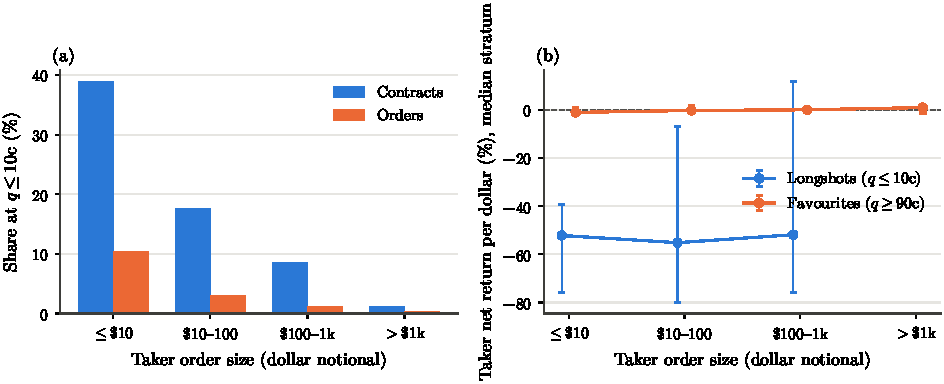
\includegraphics[width=\textwidth]{figures/fig_flow_size.pdf}
\caption{Order size and the longshot. (a) Share of taker contracts and taker orders at
$\q\le10\cents$, by order size, pooled and design-weighted. (b) Taker net return per dollar on
longshots ($\q\le10\cents$) and favourites ($\q\ge90\cents$) by order size: median across strata
with interquartile range, shown where at least six strata have five or more events in the cell
(longshot orders above \$1k qualify in only one stratum). Main sample.}\label{fig:flow-size}
% source: data/research/flb_flow/tables/size_shares.csv, size_side_strata.csv
\end{figure}

\begin{figure}[htbp]
\centering
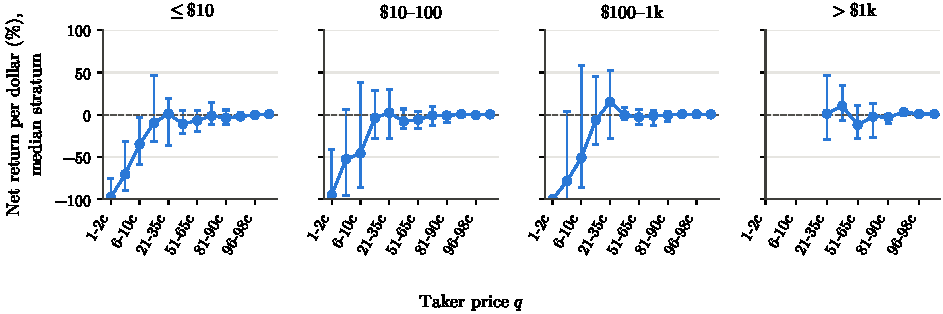
\includegraphics[width=\textwidth]{figures/fig_flow_size_buckets.pdf}
\caption{Taker net return per dollar by price bucket, one panel per order size: median across
strata with interquartile range (cells with at least six qualifying strata). Main sample.}\label{fig:flow-size-buckets}
% source: data/research/flb_flow/tables/size_returns_strata.csv
\end{figure}

\subsubsection{YES and NO takers}\label{sec:res-flow-yesno}

% source: data/research/flb_flow/tables/yesno_share.csv, yesno_strata.csv, yesno_diff.csv; summary.json (yesno_diff_side)
\paragraph{Longshot takers buy YES.} YES accounts for 79--85\% of the taker contracts bought at
$\q\le20\cents$, against 45--53\% at $\q\ge91\cents$ (\cref{tab:flow-yesno}). At equal side
price, YES-takers do worse than NO-takers in 10 of the 12 buckets of the median stratum
(\cref{fig:flow-yesno}). Examples:
\begin{itemize}
  \item at 6--10\cents{}, $-59\%$ against $-14\%$;
  \item at 11--20\cents{}, $-20\%$ against $+27\%$;
  \item at 81--90\cents{}, $-3\%$ against $+5\%$.
\end{itemize}
The pooled differences are significant at 66--80\cents{} ($-20.1$ percentage points, $t=-2.3$)
and 81--90\cents{} ($-25.8$, $t=-3.2$). For favourites as a whole the pooled difference is $-6.2$
points ($t=-1.8$). For longshots it cannot be distinguished from zero ($t=0.1$). There is a YES,
or action, bias, but it is not concentrated in the longshot buckets. The link between the two
biases is compositional: those who buy longshots overwhelmingly buy them as YES.

\begin{figure}[htbp]
\centering
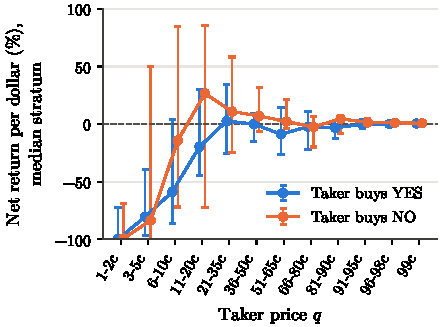
\includegraphics[width=0.55\textwidth]{figures/fig_flow_yesno.pdf}
\caption{Net return per dollar of takers who bought YES and takers who bought NO, at the same
side price: median across strata with interquartile range. Main sample.}\label{fig:flow-yesno}
% source: data/research/flb_flow/tables/yesno_strata.csv
\end{figure}

\subsubsection{Timing and attention}\label{sec:res-flow-timing}

% source: data/research/flb_flow/tables/timing.csv, timing_contrasts.csv
\paragraph{Attention does not bring in more small or longshot flow.} Small orders dominate taker
flow at every hour: about 89\% of taker orders are of at most \$100 throughout the day
(\cref{fig:flow-timing}a; every cell is listed in \cref{tab:flow-timing-cells}). In the classic attention cells (evenings, weekends, primetime games
and marquee events) neither the small-order share nor the longshot share moves significantly
(\cref{fig:flow-timing}b). The busiest cells point the other way.
\begin{itemize}
  \item In volume surges, in play, in a market's first 24 hours and in the last hour before
  expiry, the small-order share \emph{falls}, by 2--4 percentage points ($t$ between $-2.9$ and
  $-5.8$).
  \item During volume surges the longshot share of taker contracts falls by 13 points
  ($t=-2.6$).
\end{itemize}
Surges bring in relatively more large orders and fewer longshot purchases, not a retail rush
into longshots.

\paragraph{Taker returns barely move with attention.} \Cref{tab:flow-timing} compares taker
returns in each attention cell with the rest. Two contrasts are significant.
\begin{itemize}
  \item \emph{Weekends.} Taker returns are $-11.0$ points lower over all positions ($t=-2.3$) and
  $-156$ points lower on longshots ($t=-2.5$).
  \item \emph{The last hour before scheduled expiry.} The bias steepens: longshots do 172 points
  worse ($t=-3.1$) and favourites 9.0 points better ($t=2.2$).
\end{itemize}
Evening, primetime, marquee, in-play, new-listing and surge contrasts are all insignificant, with
wide intervals. Of the 24 return contrasts in \cref{tab:flow-timing}, four have $|t|>2$, and
they fall in only two cells. We therefore do not find that the bias in taker returns widens
systematically when retail attention is high, in the sense of \citet{barberodean2008} and
\citet{barber2022}. The last-hour steepening is the exception: it moves both ends of the bias in
the direction the bias predicts.

\begin{table}[htbp]
\centering
\begin{threeparttable}
\caption{Taker returns in high-attention trading}\label{tab:flow-timing}
\footnotesize
\setlength{\tabcolsep}{4pt}
\begin{tabular}{@{}lrrrrrr@{}}
\toprule
 & \multicolumn{2}{c}{All positions} & \multicolumn{3}{c}{Difference, cell minus rest (pp)} & \\
\cmidrule(lr){2-3}\cmidrule(lr){4-6}
Attention cell & In cell & Rest & All & Longshots & Favourites & Events \\
\midrule
% source: data/research/flb_flow/tables/timing_contrasts.csv
%BEGIN:timing
% source: data/research/flb_flow (generated by flb_flow tex)
Evening, 18--24 ET & $+0.9$ & $-4.4$ & $+5.3$ $(0.9)$ & $-22.3$ $(-0.4)$ & $+2.9$ $(0.6)$ & 2151 \\
Weekend (ET) & $-10.2$ & $+0.7$ & $-11.0$ $(-2.3)$ & $-156.3$ $(-2.5)$ & $+7.5$ $(1.4)$ & 2151 \\
In play (sports) & $-2.6$ & $-3.4$ & $+0.8$ $(0.1)$ & $-57.1$ $(-0.5)$ & $+2.6$ $(0.4)$ & 777 \\
Primetime game (sports) & $-3.1$ & $-2.7$ & $-0.4$ $(-0.1)$ & $-115.2$ $(-1.2)$ & $+6.2$ $(0.9)$ & 777 \\
Marquee event (top decile) & $-2.3$ & $-3.3$ & $+1.0$ $(0.2)$ & $+73.1$ $(1.1)$ & $-4.0$ $(-0.9)$ & 2151 \\
First 24 h after listing & $-5.8$ & $-1.4$ & $-4.5$ $(-0.8)$ & $+64.4$ $(0.6)$ & $-10.4$ $(-1.1)$ & 2151 \\
Volume surge ($\ge 3\times$) & $-1.5$ & $-12.9$ & $+11.3$ $(1.3)$ & $-43.5$ $(-0.5)$ & $+0.1$ $(0.0)$ & 1515 \\
Last hour before expiry & $-5.2$ & $-2.0$ & $-3.3$ $(-0.7)$ & $-172.4$ $(-3.1)$ & $+9.0$ $(2.2)$ & 2151 \\
%END:timing
\bottomrule
\end{tabular}
\begin{tablenotes}\footnotesize
\item Main sample, all groups, taker positions, design-weighted. Net return per dollar is
dollar-weighted \eqref{eq:flow-d} after the taker fee, in percent. Differences are in
percentage points, with event-clustered $t$-statistics in parentheses. In-play and primetime
contrasts are within sports games with a known scheduled start. A volume surge means the
market's volume in the preceding hour is at least three times its own past hourly average.
Marquee: the event's total volume is in the top decile of its stratum (ex post).
\end{tablenotes}
\end{threeparttable}
\end{table}

\begin{figure}[htbp]
\centering
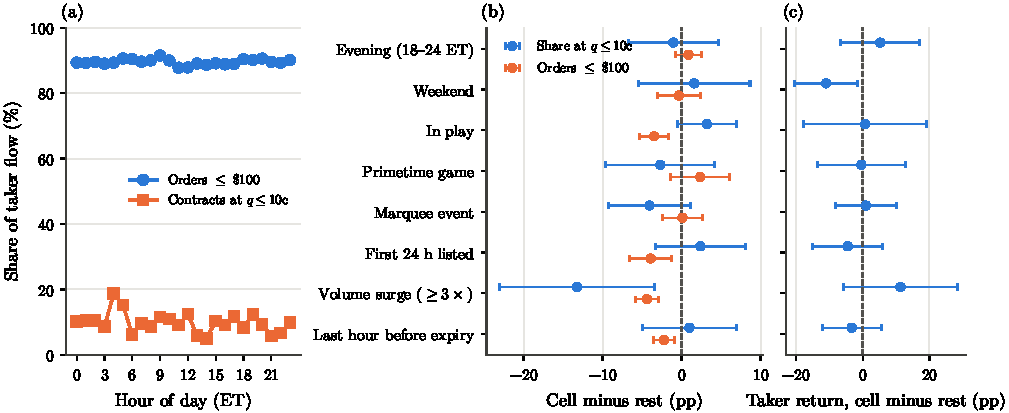
\includegraphics[width=\textwidth]{figures/fig_flow_timing.pdf}
\caption{Timing and attention. (a) Share of taker orders of at most \$100 and share of taker
contracts at $\q\le10\cents$, by hour of day (ET). (b) Each attention cell minus the rest: the
share of taker contracts at $\q\le10\cents$ and the share of taker orders of at most \$100, in
percentage points. (c) Each attention cell minus the rest: taker net return per dollar over all
positions. 95\% confidence intervals clustered by event. Main sample, design-weighted.}\label{fig:flow-timing}
% source: data/research/flb_flow/tables/timing.csv, timing_contrasts.csv
\end{figure}

\subsubsection{Order flow, price impact and information}\label{sec:res-flow-impact}

% source: data/research/flb_flow/tables/markouts.csv, markouts_strata.csv, decomp_side.csv; summary.json (hourly, markouts_coverage)
\paragraph{Price impact rises with size.} These results use the prints with a tight mid-quote
proxy before and after the order: 36\% of contracts, concentrated in the more liquid markets.
\begin{itemize}
  \item Every size bucket pays a similar effective half-spread, 0.56--0.68\cents{} per contract
  ($t>16$; \cref{tab:flow-markouts}).
  \item One minute after the order, the mid has moved in the taker's direction by 0.04\cents{}
  for orders of at most \$10 and by 0.41\cents{} for orders above \$1k ($t$ from 2.5 to 4.9).
  \item One hour later, the median-stratum impact is 0.20, 0.66, 1.78 and 0.39\cents{} across
  the four size buckets.
\end{itemize}

\paragraph{Market-hour order flow.} Regression~\eqref{eq:flow-reg} uses the 15,740
market-hours, in 651 events, with a tight proxy at both ends of the hour (\cref{tab:flow-oib},
\cref{fig:flow-impact}).
\begin{itemize}
  \item \emph{Same hour.} An hour of entirely one-sided taker flow moves the mid by 0.28\cents{}
  if it is small ($t=2.6$), 2.74\cents{} if medium ($t=7.4$) and 3.26\cents{} if large
  ($t=5.3$).
  \item \emph{Next hour.} Small and medium flow keep moving the price in the same direction
  (0.35\cents, $t=2.8$; 0.58\cents, $t=2.6$). The impact of large flow neither continues nor
  reverts ($-0.08$\cents, $t=-0.2$), while the mid itself partly reverses (coefficient on the
  same-hour change $-0.12$, $t=-2.2$).
  \item \emph{To settlement.} No size class predicts the outcome. The estimates are 3.3\cents{}
  for small flow ($t=1.3$), $-0.4\cents$ for medium ($t=-0.3$) and $-11.3\cents$ for large
  ($t=-1.6$).
\end{itemize}

\paragraph{Small flow is neither informed nor noise that reverts.} Small taker flow moves prices
little and does not predict outcomes, but its impact does not reverse within the hour either.
This differs from equity markets, where the net buying of individual investors predicts
returns over the following weeks \citep{kanielsaartitman2008,boehmer2021}.
Large flow moves prices most, as the depth of a \citet{kyle1985} market implies, but the
outcome does not confirm its direction. If anything, the point estimate goes against it, in
sports and non-sports alike. The per-order markouts to settlement are noisy and centred near
zero (median stratum between $-0.7$ and $+2.7\cents$). Combined with the immediacy cost above,
this explains the taker's loss on longshots as a liquidity cost, not as adverse selection
against informed makers. Takers lose because they pay the spread and the fee on cheap
contracts. They do not lose because the side they buy predictably moves against them.

\begin{table}[htbp]
\centering
\begin{threeparttable}
\caption{Price impact and markouts of taker orders by size (cents per contract)}\label{tab:flow-markouts}
\footnotesize
\begin{tabular}{@{}lrrrrr@{}}
\toprule
Order size & Half-spread $s$ & Impact $I_{1m}$ & Impact $I_{1h}$ & Markout $M_{1h}$ & Markout $M_\infty$ \\
\midrule
% source: data/research/flb_flow/tables/markouts.csv
%BEGIN:markouts
% source: data/research/flb_flow (generated by flb_flow tex)
$\le$\$10 & $+0.56$ $(21.2)$ & $+0.04$ $(2.5)$ & $+3.43$ $(2.6)$ & $+2.87$ $(2.1)$ & $+21.69$ $(1.7)$ \\
\$10--100 & $+0.58$ $(19.6)$ & $+0.10$ $(3.5)$ & $+2.91$ $(2.3)$ & $+2.33$ $(1.8)$ & $+13.28$ $(1.3)$ \\
\$100--1k & $+0.68$ $(18.3)$ & $+0.19$ $(4.9)$ & $+1.03$ $(1.6)$ & $+0.35$ $(0.5)$ & $+2.18$ $(0.5)$ \\
$>$\$1k & $+0.68$ $(16.8)$ & $+0.41$ $(4.1)$ & $-1.40$ $(-1.4)$ & $-2.08$ $(-2.1)$ & $-6.86$ $(-0.8)$ \\
%END:markouts
\bottomrule
\end{tabular}
\begin{tablenotes}\footnotesize
\item Main sample, all groups, taker prints with a mid-quote proxy no wider than 5\cents{} just
before the order and a proxy one minute and one hour after it. Contract-weighted and design-weighted, in cents per contract, from
the taker's side \eqref{eq:flow-markout}. $M_\infty$ is the gross profit to settlement. $t$-statistics
clustered by event are in parentheses.
\end{tablenotes}
\end{threeparttable}
\end{table}

\begin{table}[htbp]
\centering
\begin{threeparttable}
\caption{Spread or price? Decomposing the taker's gross loss (cents per contract)}\label{tab:flow-decomp}
\footnotesize
\setlength{\tabcolsep}{4pt}
\begin{tabular}{@{}llrrrrrr@{}}
\toprule
 & & Mean $\q$ & Gross profit & Mid to outcome & Half-spread & Fee & Immediacy \\
Sample & Taker side & (\cents) & $d(Y-p)$ & $d(Y-m_{t^-})$ & $s$ & $\fee^T$ & cost (\%/\$) \\
\midrule
% source: data/research/flb_flow/tables/decomp_side.csv
%BEGIN:decomp
% source: data/research/flb_flow (generated by flb_flow tex)
Sports & Longshots ($\q\le10\cents$) & $5.5$ & $+2.00$ $(0.6)$ & $+2.51$ $(0.8)$ & $+0.50$ $(14.0)$ & $0.33$ & $14.2$ \\
 & Middle & $49.4$ & $-0.15$ $(-0.1)$ & $+0.64$ $(0.3)$ & $+0.78$ $(13.0)$ & $1.34$ & $4.2$ \\
 & Favourites ($\q\ge90\cents$) & $94.9$ & $-2.52$ $(-0.6)$ & $-1.51$ $(-0.4)$ & $+1.02$ $(11.0)$ & $0.32$ & $1.4$ \\
Non-sports & Longshots ($\q\le10\cents$) & $3.8$ & $-0.17$ $(-0.1)$ & $+0.45$ $(0.3)$ & $+0.62$ $(11.7)$ & $0.25$ & $21.2$ \\
 & Middle & $47.8$ & $+1.61$ $(0.9)$ & $+3.94$ $(2.8)$ & $+2.34$ $(6.0)$ & $1.31$ & $7.4$ \\
 & Favourites ($\q\ge90\cents$) & $96.9$ & $-2.05$ $(-0.6)$ & $+0.56$ $(0.2)$ & $+2.61$ $(5.3)$ & $0.21$ & $2.9$ \\
All & Longshots ($\q\le10\cents$) & $5.5$ & $+1.94$ $(0.6)$ & $+2.44$ $(0.8)$ & $+0.51$ $(14.4)$ & $0.33$ & $14.4$ \\
 & Middle & $49.4$ & $-0.14$ $(-0.1)$ & $+0.65$ $(0.3)$ & $+0.79$ $(12.8)$ & $1.34$ & $4.2$ \\
 & Favourites ($\q\ge90\cents$) & $95.0$ & $-2.51$ $(-0.6)$ & $-1.44$ $(-0.4)$ & $+1.07$ $(10.8)$ & $0.32$ & $1.5$ \\
%END:decomp
\bottomrule
\end{tabular}
\begin{tablenotes}\footnotesize
\item Main sample, taker prints with a mid-quote proxy no wider than 5\cents{} just before the
order. Contract-weighted and design-weighted, in cents per contract, with event-clustered
$t$-statistics in parentheses. By construction the gross profit equals the mid-to-outcome term
minus the half-spread. The first term is the bias in the quoted price that any buyer of the
side faces, and the second is the cost of immediacy. Fee: the exact taker fee per contract.
Immediacy cost: $(s+\fee^T)/(\q+\fee^T)$, dollar-weighted, in percent of the stake.
\end{tablenotes}
\end{threeparttable}
\end{table}

\begin{table}[htbp]
\centering
\begin{threeparttable}
\caption{Signed taker imbalance by size class and subsequent mid-quote changes}\label{tab:flow-oib}
\footnotesize
\setlength{\tabcolsep}{4pt}
\begin{tabular}{@{}llrrrrrr@{}}
\toprule
 & & \multicolumn{3}{c}{Imbalance $\mathrm{OIB}_c$} & Same-hour & Market- & \\
\cmidrule(lr){3-5}
Sample & Change & Small & Medium & Large & change & hours & Events \\
\midrule
% source: data/research/flb_flow/summary.json (hourly)
%BEGIN:oib
% source: data/research/flb_flow (generated by flb_flow tex)
All & Same hour & $+0.28$ $(2.6)$ & $+2.74$ $(7.4)$ & $+3.26$ $(5.3)$ & -- & 15,740 & 651 \\
 & Next hour & $+0.35$ $(2.8)$ & $+0.58$ $(2.6)$ & $-0.08$ $(-0.2)$ & $-0.12$ $(-2.2)$ & 9,611 & 381 \\
 & To settlement & $+3.28$ $(1.3)$ & $-0.45$ $(-0.3)$ & $-11.26$ $(-1.6)$ & $+0.01$ $(0.2)$ & 15,740 & 651 \\
Sports & Same hour & $-0.63$ $(-1.3)$ & $+1.84$ $(3.6)$ & $+2.87$ $(3.6)$ & -- & 3,281 & 308 \\
 & Next hour & $+0.66$ $(1.1)$ & $+0.33$ $(0.7)$ & $-0.06$ $(-0.1)$ & $-0.43$ $(-2.6)$ & 2,084 & 173 \\
 & To settlement & $+8.24$ $(1.2)$ & $+1.20$ $(0.2)$ & $-6.50$ $(-0.8)$ & $+0.02$ $(0.3)$ & 3,281 & 308 \\
Non-sports & Same hour & $+0.45$ $(4.0)$ & $+3.11$ $(5.9)$ & $+3.64$ $(3.8)$ & -- & 12,459 & 343 \\
 & Next hour & $+0.25$ $(2.1)$ & $+0.44$ $(1.8)$ & $+0.05$ $(0.2)$ & $-0.02$ $(-0.4)$ & 7,527 & 208 \\
 & To settlement & $+2.61$ $(1.0)$ & $-0.76$ $(-0.5)$ & $-13.50$ $(-1.4)$ & $+0.00$ $(0.1)$ & 12,459 & 343 \\
%END:oib
\bottomrule
\end{tabular}
\begin{tablenotes}\footnotesize
\item OLS of regression~\eqref{eq:flow-reg} on market-hours with taker volume and a tight
($\le5\cents$) mid-quote proxy at both ends of the hour (and of the next hour, for the next-hour
change). The dependent
variable is in cents. The imbalances~\eqref{eq:flow-oib} are signed contracts of each size
class (small $\le\$100$, medium $\$100$--$1$k, large $>\$1$k) over the hour's volume. Same-hour
change: the control $m^{\mathrm{end}}_h-m^{\mathrm{start}}_h$. $t$-statistics (CR1, clustered
by event) are in parentheses. Market-hours are unweighted.
\end{tablenotes}
\end{threeparttable}
\end{table}

\begin{figure}[htbp]
\centering
\begin{subfigure}[t]{0.58\textwidth}
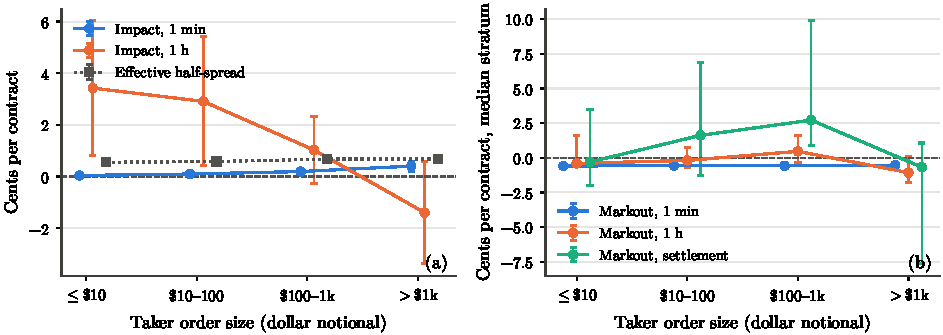
\includegraphics[width=\textwidth]{figures/fig_flow_markouts.pdf}
\end{subfigure}
\hfill
\begin{subfigure}[t]{0.40\textwidth}
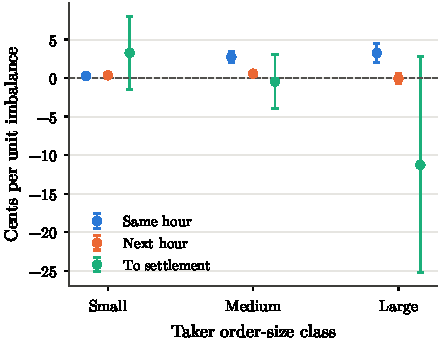
\includegraphics[width=\textwidth]{figures/fig_flow_oib.pdf}
\end{subfigure}
\caption{Price impact and information. Left: (a) effective half-spread and price impact at
one minute and one hour (pooled, design-weighted, 95\% intervals clustered by event), and (b)
taker markouts at one minute, one hour and settlement (median across strata with interquartile
range), by taker order size, in cents per contract. Right: coefficients of
regression~\eqref{eq:flow-reg} on the signed imbalance of each size class, for the same-hour
change, the next-hour change and the drift to settlement, with 95\% intervals clustered by
event.}\label{fig:flow-impact}
% source: data/research/flb_flow/tables/markouts.csv, markouts_strata.csv, summary.json (hourly)
\end{figure}

\subsubsection{Robustness}\label{sec:res-flow-robust}

% source: data/research/flb_flow/summary.json (robust, sign_tests)
\Cref{tab:flow-robust} repeats the headline numbers in subsamples. The results that hold
everywhere are the size gradient in longshot buying and the absence of a taker--maker gap
averaged over all prices.
\begin{itemize}
  \item \emph{Size gradient.} The longshot share of orders of at most \$10 exceeds that of
  orders above \$1k by 28 to 57 points in both halves, under the strict rule and in the
  replication sample.
  \item \emph{No overall taker--maker gap.} Pooled taker returns lie between $-0.9$ and
  $-3.5\%$ and maker returns between $-1.4$ and $+0.5\%$. Neither is significant in any
  variant. Clustering by market instead of event leaves the difference insignificant
  ($t=-0.1$).
  \item \emph{Pooled longshot returns are unstable.} The pooled taker return on longshots is
  $-35\%$ in the first half and $+125\%$ in the second. The second half contains the MLB
  home-run prop that dominates the pooled sports estimate.
  \item \emph{Small-order longshots.} Without design weights, longshot positions in orders of at
  most \$10 lose 28\% ($t=-2.2$). In the replication sample, which is a much larger set of
  prints, they lose 37\% ($t=-1.9$).
  \item \emph{Excluded prices.} Dropping 1--2\cents{} and 99\cents{} prints changes nothing
  material.
\end{itemize}

\begin{table}[htbp]
\centering
\begin{threeparttable}
\caption{Headline results across subsamples and weights}\label{tab:flow-robust}
\footnotesize
\setlength{\tabcolsep}{3.5pt}
\begin{tabular}{@{}lrrrrrr@{}}
\toprule
 & \multicolumn{2}{c}{All positions} & \multicolumn{3}{c}{Taker longshots ($\q\le10\cents$)} & \LS{} share (\%) \\
\cmidrule(lr){2-3}\cmidrule(lr){4-6}
Sample & Taker & Maker & All orders & $\le\$10$ orders & $>\$1$k orders & $\le\$10$ / $>\$1$k \\
\midrule
% source: data/research/flb_flow/summary.json (headline, robust)
%BEGIN:robust
% source: data/research/flb_flow (generated by flb_flow tex)
Main sample & $-2.4$ $(-0.7)$ & $-0.4$ $(-0.1)$ & $+48.9$ $(1.0)$ & $+30.6$ $(0.8)$ & $+164.3$ $(1.2)$ & $39$ / $1$ \\
First half (by close) & $-1.2$ $(-0.2)$ & $-1.4$ $(-0.2)$ & $-34.9$ $(-1.1)$ & $-30.2$ $(-1.0)$ & $-99.9$ $(-1853.9)$ & $41$ / $1$ \\
Second half & $-3.5$ $(-1.3)$ & $+0.5$ $(0.2)$ & $+124.8$ $(1.7)$ & $+75.2$ $(1.3)$ & $+323.5$ $(1.6)$ & $37$ / $1$ \\
Strict pre-resolution & $-3.1$ $(-0.3)$ & $+0.1$ $(0.0)$ & $+105.9$ $(1.2)$ & $+109.4$ $(1.3)$ & $+65.3$ $(0.4)$ & $30$ / $2$ \\
Excluding 1--2\cents{} and 99\cents & $-2.5$ $(-0.7)$ & $-0.4$ $(-0.1)$ & $+50.5$ $(1.0)$ & $+39.9$ $(0.8)$ & $+164.4$ $(1.2)$ & $27$ / $1$ \\
No design weights & $-2.1$ $(-1.2)$ & $-0.3$ $(-0.2)$ & $-8.0$ $(-0.4)$ & $-28.4$ $(-2.2)$ & $-1.2$ $(-0.0)$ & $57$ / $2$ \\
Sports & $-2.4$ $(-0.7)$ & $-0.4$ $(-0.1)$ & $+52.0$ $(1.0)$ & $+36.1$ $(0.8)$ & $+169.0$ $(1.2)$ & $36$ / $1$ \\
Non-sports & $-0.9$ $(-1.0)$ & $-0.4$ $(-0.5)$ & $-31.0$ $(-1.5)$ & $-35.2$ $(-1.3)$ & $-85.1$ $(-4.6)$ & $74$ / $3$ \\
Replication sample & $-3.0$ $(-0.7)$ & $+0.2$ $(0.1)$ & $+6.2$ $(0.2)$ & $-36.6$ $(-1.9)$ & $+40.3$ $(0.7)$ & $62$ / $5$ \\
Replication, strict & $-3.2$ $(-0.8)$ & $+0.4$ $(0.1)$ & $+12.5$ $(0.4)$ & $-24.2$ $(-1.0)$ & $-5.5$ $(-0.1)$ & $52$ / $5$ \\
%END:robust
\bottomrule
\end{tabular}
\begin{tablenotes}\footnotesize
\item Net return per dollar, dollar-weighted \eqref{eq:flow-d} after each role's fee, in
percent, with event-clustered $t$-statistics in parentheses. Halves split the main sample's
markets at their median close time. Strict pre-resolution keeps only pre-game sports prints and
other prints more than 24 hours before the close. The replication sample is the separate set
of prints described in \cref{sec:data-flow}, which carries no design weights. \LS{} share: the
share of taker contracts at $\q\le10\cents$ in orders of at most \$10 and of more than \$1k.
\end{tablenotes}
\end{threeparttable}
\end{table}

\paragraph{Summary.} The trade-level evidence partly supports the preference and retail-demand
hypothesis (\cref{hyp:pref}).
\begin{itemize}
  \item Small takers are the longshot buyers. The size gradient holds in every stratum, and
  takers buy most longshots, mainly as YES.
  \item Takers lose more than makers on longshots. They pay a spread and a fee that together
  cost about 14\% of the stake at the average longshot price of 5.5\cents.
  \item But the per-dollar loss on a longshot is about the same for small and larger orders, and
  attention does not systematically widen it.
\end{itemize}
The information hypothesis (\cref{hyp:info}) finds no support at the trade level. Neither small
nor large taker flow predicts outcomes beyond the price. The resting side of a longshot trade
earns the spread; it is not exploiting the taker's ignorance of the outcome. Who pays the bias is
therefore mostly a question of who demands immediacy on cheap contracts, and on Kalshi that is
small takers.

\subsection{Wallets, retail traders and venues}\label{sec:res-wallets}
% Wallets workstream: results. Every number traces to data/research/flb_wallets/ (file named per paragraph).
This subsection answers the four questions of the wallets workstream in turn: how Polymarket prices
longshots, which wallets buy them, how concentrated and persistent wallet profits are, and how
retail inflows and cross-venue prices behave.

\subsubsection{Polymarket calibration and the bias by group}\label{sec:res-wallets-calib}

% source: data/research/flb_wallets/calib_slopes.csv, calib_market.csv
\Cref{tab:wallets-calib} and \cref{fig:wallets-calib} summarise calibration on Polymarket. Measured 24 hours before the
information time, the pooled calibration slope is $\hat\beta=0.99$ (SE 0.15; 2{,}121
markets), so $\beta=1$ is not rejected ($t=-0.1$). The slope is 0.91 (SE 0.14) one hour
before and 0.84 (SE 0.17) a week before. Weighting every sampled market equally gives
0.97 (SE 0.05). The slope is 1.28 in H1 and 0.97 in H2. By group, the 24-hour
slopes are Sports 1.00, Politics 1.15, Weather 0.71, Entertainment 1.20, Mentions 0.84, Science \& Tech 0.99, Other 0.82; 7 of the 7 are within two standard errors of one (\cref{tab:wallets-calib}).

Returns by price bucket are noisier. Buying every side priced at most 10\cents{} 24 hours
ahead returns 84.5\% ($t=0.5$) per dollar market-weighted, $-$16.5\% ($t=-0.2$) volume-weighted and 64.9\% ($t=0.8$) with equal weights. Buying
every side priced at least 90\cents{} returns 1.9\% ($t=2.5$) and 2.3\% ($t=4.8$). Longshot returns are imprecise because a
handful of 1--2\cents{} winners carry large design weights. The calibration slope pools all price levels and is the
more reliable summary.

% source: data/research/flb_wallets/trade_flb.csv (ret_n, dollar-weighted)
At the level of fills the bias is clear. Buying a longshot before the information time and holding it to
settlement returns $-$53.8\% ($t=-2.8$) per dollar net of fees; buying a favourite returns 2.2\% ($t=3.5$). The signs are the
same in every group: longshot buys lose between 48\% and 71\% per dollar (significant at
5\% in 5 of the 7 groups), and favourite buys earn between 1.1\% and 3.5\%
(significant in 4; \cref{tab:wallets-calib}). The longshot loss is larger for takers ($-$71.2\% ($t=-5.9$)) than for
makers ($-$33.3\% ($t=-1.2$)), and larger in H1 ($-$90.9\% ($t=-18.7$)) than in H2 ($-$30.2\% ($t=-1.0$)). Favourites earn 3.9\% ($t=6.9$) in H1 and
1.4\% ($t=1.7$) in H2. The two measures weight markets and moments differently. The fill-level return weights each
dollar actually spent, including purchases in the last hours before the information time. The market-level
calibration takes one price per market a day ahead, where the bias is weak. \Cref{sec:res-xs} reports
the corresponding Kalshi estimates.

\begin{figure}[t]
\centering
% source: data/research/flb_wallets/calib_market.csv, trade_flb.csv
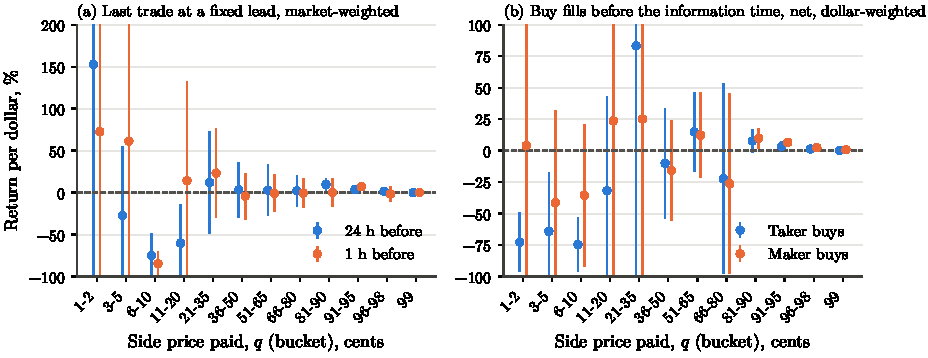
\includegraphics[width=\textwidth]{figures/fig_wallets_calib.pdf}
\caption{Return per dollar by side-price bucket on Polymarket. (a) Last trade 24 hours and 1 hour before the information time, both sides of each market, market-weighted with design weights, gross. (b) Buy fills before the information time held to settlement, net of taker fees, dollar-weighted, by liquidity role. Bars are 95\% confidence intervals clustered by event, truncated at the axis limits.}\label{fig:wallets-calib}
\end{figure}

\begin{table}[t]
\centering
\small
\begin{threeparttable}
\caption{Polymarket calibration and longshot returns by group}\label{tab:wallets-calib}
\footnotesize
\setlength{\tabcolsep}{4pt}
% source: data/research/flb_wallets/calib_slopes.csv, calib_market.csv (lead_h=24, market-weighted), trade_flb.csv (ret_n, dollar)
\begin{tabular}{lrcccccc}
\toprule
& & \multicolumn{4}{c}{Last trade 24\,h before $t^{\mathrm{info}}$} & \multicolumn{2}{c}{Buy fills before $t^{\mathrm{info}}$} \\
\cmidrule(lr){3-6}\cmidrule(lr){7-8}
& & $\hat\beta$ (SE) & $\hat\beta$ (SE) & $\ret$, \LS & $\ret$, \FAV & $\ret$, \LS & $\ret$, \FAV \\
& Markets & design & sample & \% ($t$) & \% ($t$) & \% ($t$) & \% ($t$) \\
\midrule
All markets & 2{,}121 & 0.99 (0.15) & 0.97 (0.05) & 84.5 (0.5) & 1.9 (2.5) & $-$53.8 ($-$2.8) & 2.2 (3.5) \\
\addlinespace
Sports & 285 & 1.00 (0.24) & 1.08 (0.18) & $-$93.6 ($-$20.3) & 5.7 (3.6) & $-$60.1 ($-$2.2) & 3.3 (2.0) \\
Politics & 416 & 1.15 (0.18) & 1.05 (0.13) & $-$80.3 ($-$8.3) & 0.4 (0.5) & $-$48.0 ($-$1.5) & 2.1 (2.0) \\
Weather & 303 & 0.71 (0.25) & 0.74 (0.14) & 257.7 (0.7) & 0.4 (0.5) & $-$70.6 ($-$6.2) & 1.4 (7.1) \\
Entertainment & 406 & 1.20 (0.19) & 1.24 (0.15) & $-$84.4 ($-$8.3) & 1.2 (2.4) & $-$59.2 ($-$3.9) & 2.0 (3.2) \\
Mentions & 227 & 0.84 (0.14) & 0.77 (0.13) & $-$88.3 ($-$7.3) & 6.7 (7.7) & $-$57.4 ($-$2.8) & 3.5 (1.6) \\
Science \& Tech & 289 & 0.99 (0.16) & 1.04 (0.13) & $-$26.1 ($-$0.5) & $-$1.2 ($-$0.7) & $-$61.0 ($-$2.8) & 1.1 (1.8) \\
Other & 195 & 0.82 (0.15) & 0.89 (0.13) & 18.3 (0.3) & $-$3.4 ($-$1.4) & $-$49.1 ($-$1.6) & 1.4 (1.4) \\
\addlinespace
H1 & 912 & 1.28 (0.16) & 1.06 (0.09) & $-$36.1 ($-$1.5) & 0.2 (0.2) & $-$90.9 ($-$18.7) & 3.9 (6.9) \\
H2 & 1{,}209 & 0.97 (0.16) & 0.91 (0.06) & 93.3 (0.5) & 2.0 (2.5) & $-$30.2 ($-$1.0) & 1.4 (1.7) \\
\bottomrule
\end{tabular}
\begin{tablenotes}\footnotesize
\item Sample: stratified random sample of resolved in-scope Polymarket markets (\$1k--\$6M), January 2024
  to October 2026. Left block: one observation per side of each market with a trade at least 24\,h before
  its information time $t^{\mathrm{info}}$; $\beta$ from \eqref{eq:logit} on the outcome-0 side, with design
  weights or with every sampled market weighted equally (``sample''); \LS: $\q\le10\cents$, \FAV: $\q\ge90\cents$; returns
  $\ret$ in \% per dollar, gross (Polymarket charged no fees before 2026), market-weighted (design weights).
  H1: markets resolving January 2024 to May 2025; H2: June 2025 to October 2026.
  Right block: buy fills (maker and taker) before $t^{\mathrm{info}}$, held to settlement, \% per dollar
  net of taker fees, dollar-weighted (notional $\times$ design weight). $t$-statistics in parentheses;
  standard errors clustered by event.
\end{tablenotes}
\end{threeparttable}
\end{table}

\subsubsection{Who buys longshots}\label{sec:res-wallets-who}

% source: data/research/flb_wallets/who_share.csv (dim=cls), ls_flow.csv, class_pnl.csv
\Cref{tab:wallets-class} describes the five classes. Occasional small wallets (``retail'') make
31.3\% of buy fills and 12.4\% of dollars bought, across 175{,}734 wallets.
Market-maker-like wallets make 33.3\% of fills, and whales 21.9\% of dollars from only
1{,}677 wallets.

Longshots are a large share of what small wallets and market makers \emph{buy}, but a small share of what
any class \emph{spends}:
\begin{itemize}
  \item Longshots are 11.5\% of retail buy fills, 15.7\% of active-retail fills and 21.8\% of
    market-maker fills, but only 1.5\% of mid-size and 0.2\% of whale fills
    (\cref{fig:wallets-lsshare}).
  \item Because longshots are cheap, they are at most 1.3\% of any
    class's dollars bought.
  \item Favourites take between 5.7\% and
    14.8\% of each class's dollars: most for
    active retail and retail, least for whales.
\end{itemize}

Net flows show who takes the other side. Counting every buy and sell before the information time,
retail wallets are the clear net buyers of longshots: 0.43\% of the dollars they trade
($t=3.9$), as takers (0.47\%, $t=2.7$) and with resting orders (0.39\%,
$t=2.4$). Net flows sum to zero across classes, and retail makes 86\% of all net longshot
buying. The other classes are close to flat on net: active retail 0.04\% ($t=0.4$), mid-size wallets $-$0.06\% ($t=-1.0$), whales $-$0.06\% ($t=-1.6$), market makers $-$0.16\% ($t=-1.3$). None of these is individually significant
($|t|\leq1.6$). The longshot buying of small, occasional wallets is thus absorbed by many counterparties,
not by one class of professional sellers. That small accounts tilt towards lottery-like payoffs matches the evidence on
individual investors in equity markets \citep{kumar2009}.

The returns on these purchases differ by class (\cref{fig:wallets-classret}). Per dollar, net longshot returns
are $-$36.3\% ($t=-1.4$) for retail, $-$59.4\% ($t=-3.0$) for active retail and $-$42.3\% ($t=-1.6$) for market makers;
the few longshots bought by mid-size wallets and whales lose 90\% and 100\% of
their cost. Across all
price levels, class PnL per dollar traded is $-$2.1\% ($t=-0.8$) for retail, 14.1\% ($t=2.5$) for
active retail, $-$6.3\% ($t=-1.2$) for mid-size wallets, 5.3\% ($t=1.1$) for whales and $-$10.8\% ($t=-1.4$) for market
makers (\cref{tab:wallets-class}). Only the figure for active retail is significant at the 5\% level.
\Cref{tab:wallets-robust} in \cref{app:wallets} shows that the ordering of longshot shares survives every change of cut-off.

% source: data/research/flb_wallets/who_share.csv (dims size_bucket, lb)
Fill size gives the same gradient without any classification (\cref{tab:wallets-sizeage}). Longshots are
23.1\% of buy fills of at most \$10, 2.4\% of \$10--100 fills,
0.7\% of \$100--1k fills and 0.2\% of fills above \$1{,}000. Per dollar,
however, the small longshot purchases lose least: $-$22.2\% ($t=-0.6$) for fills of at most \$10,
against $-$48.4\% ($t=-2.4$) at \$10--100 and $-$77.6\% ($t=-4.5$) at
\$100--1k. All-time
leaderboard wallets put 6.8\% of their buy fills into longshots, against 15.4\% for other
wallets.

% source: data/research/flb_wallets/hold_exit.csv
Do longshot buyers hold to settlement? \Cref{tab:wallets-holdexit} in \cref{app:wallets} follows each position
opened by a buy. Retail sells at least half of 41.7\% of its longshot positions before the close, active
retail 6.9\% and market makers 54.7\%. For longshot entries, the realised PnL exceeds
the hold-to-settlement PnL by 23.2\% ($t=2.2$) of cost: the shares sold were worth less at settlement than their sale
price, as expected if longshots are overpriced when they are sold. Across all positions the difference is
$-$1.4\% ($t=-1.3$), and for favourite entries $-$1.2\% ($t=-2.1$). Selling favourites early forgoes some of their small
positive return.

\begin{figure}[t]
\centering
% source: data/research/flb_wallets/who_share.csv
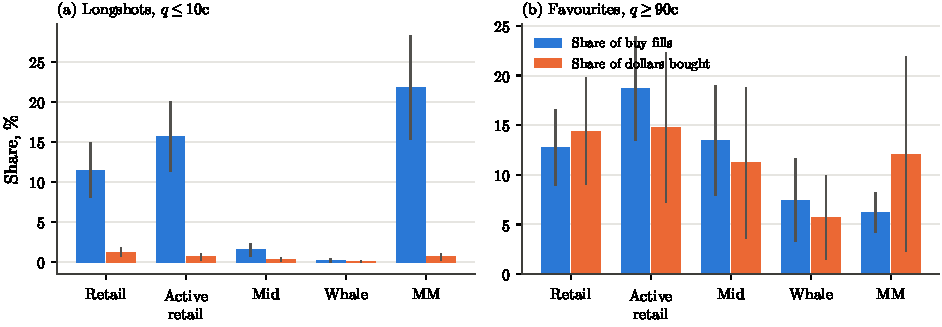
\includegraphics[width=\textwidth]{figures/fig_wallets_lsshare.pdf}
\caption{Longshot ($q\le10$c) and favourite ($q\ge90$c) shares of buying by wallet class: share of design-weighted buy fills and of dollars bought, buy fills before the information time. Bars are 95\% confidence intervals clustered by event.}\label{fig:wallets-lsshare}
\end{figure}

\begin{figure}[t]
\centering
% source: data/research/flb_wallets/who_class_cbucket.csv
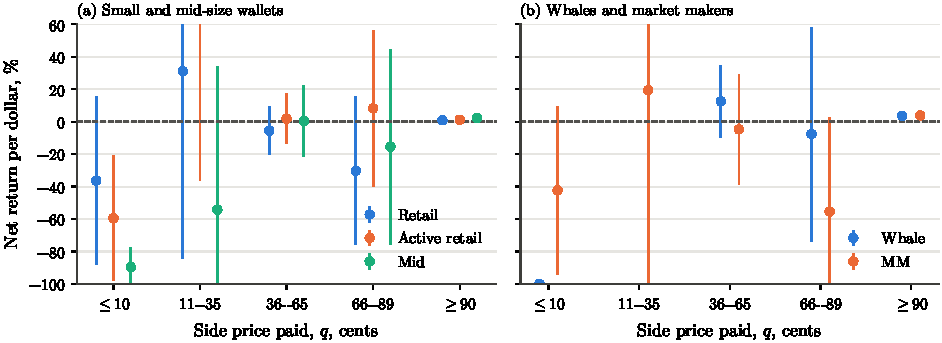
\includegraphics[width=\textwidth]{figures/fig_wallets_classret.pdf}
\caption{Net return per dollar of buy fills by wallet class and side price, held to settlement, dollar-weighted, buy fills before the information time. Bars are 95\% confidence intervals clustered by event.}\label{fig:wallets-classret}
\end{figure}

\begin{table}[t]
\centering
\small
\begin{threeparttable}
\caption{Who buys longshots: buying, returns and PnL by wallet class}\label{tab:wallets-class}
% source: data/research/flb_wallets/who_share.csv (dim=cls, half=All), ls_flow.csv (half=All, role=all), class_pnl.csv (half=All)
\footnotesize
\setlength{\tabcolsep}{4pt}
\begin{tabular}{lrrrrrrccc}
\toprule
& & \multicolumn{2}{c}{Share of buying} & \multicolumn{2}{c}{\LS{} share} & \FAV{} share & \LS{} $\ret$ & Net \LS{} flow & PnL per \$ \\
\cmidrule(lr){3-4}\cmidrule(lr){5-6}\cmidrule(lr){7-7}\cmidrule(lr){8-8}\cmidrule(lr){9-9}\cmidrule(lr){10-10}
Class & Wallets & fills & \$ & fills & \$ & \$ & \% ($t$) & \% ($t$) & \% ($t$) \\
\midrule
Retail & 175{,}734 & 31.3 & 12.4 & 11.5 & 1.3 & 14.4 & $-$36.3 ($-$1.4) & 0.43 (3.9) & $-$2.1 ($-$0.8) \\
Active retail & 6{,}431 & 31.9 & 24.1 & 15.7 & 0.7 & 14.8 & $-$59.4 ($-$3.0) & 0.04 (0.4) & 14.1 (2.5) \\
Mid & 15{,}393 & 3.2 & 20.5 & 1.5 & 0.3 & 11.2 & $-$89.6 ($-$14.9) & $-$0.06 ($-$1.0) & $-$6.3 ($-$1.2) \\
Whale & 1{,}677 & 0.2 & 21.9 & 0.2 & 0.1 & 5.7 & $-$100.0 ($<-$100) & $-$0.06 ($-$1.6) & 5.3 (1.1) \\
MM & 3{,}589 & 33.3 & 21.1 & 21.8 & 0.7 & 12.1 & $-$42.3 ($-$1.6) & $-$0.16 ($-$1.3) & $-$10.8 ($-$1.4) \\
\bottomrule
\end{tabular}
\begin{tablenotes}\footnotesize
\item Classes are assigned to each fill from the wallet's history before it (\cref{sec:method-wallets}).
  Wallets: distinct wallets with at least one buy in the class (a wallet can change class over time).
  Shares of buying and longshot ($\q\le10\cents$) / favourite ($\q\ge90\cents$) shares use buy fills before
  $t^{\mathrm{info}}$, in \% of design-weighted fills or dollars. Longshot $\ret$: net return per dollar of
  those longshot buys held to settlement, dollar-weighted. Net LS flow: net longshot dollars bought per
  dollar traded (buys and sells, both roles; positive = net buyer of longshots). PnL per \$: exact
  wallet-market PnL \eqref{eq:wallets-pnl} net of fees per dollar traded, class at the wallet's first fill
  in the market. $t$-statistics clustered by event.
\end{tablenotes}
\end{threeparttable}
\end{table}

\subsubsection{Profit concentration and persistence}\label{sec:res-wallets-skill}

% source: data/research/flb_wallets/summary.json:concentration
The accounting identity holds in the data. In 99.95\% of the
2{,}197 fee-free markets the PnL of all wallets sums to zero within $10^{-6}$ of turnover, and the
YES-equivalent positions sum to zero in 97.8\%. In fee markets the residual is
the fee charged in shares. PnL is therefore a transfer between wallets. Of 237{,}569
wallets, 50.7\% end with positive PnL in the sampled markets. The gains are highly
concentrated (\cref{tab:wallets-skill}, \cref{fig:wallets-lorenz}):
\begin{itemize}
  \item the top 1\% of wallets take 85\% of all gains and the top 0.1\%
    take 51\%;
  \item 220 wallets hold half of all gains;
  \item the Gini coefficient of gains among winners is 0.97.
\end{itemize}
Losses are less concentrated (Gini 0.95; 326 wallets
for half of all losses), and dollar volume is concentrated to a similar degree (Gini 0.96).
The 96 all-time leaderboard wallets in the sample take 11.8\% of gains on
10.4\% of volume. \citet{akey2026} report a similar concentration of profits across all
Polymarket users, and equity markets show the same pattern of losses spread over many individual traders
\citep{barberodean2000,barberleeliuodean2009}.

% source: data/research/flb_wallets/summary.json:persistence, persistence.csv
Concentration alone does not show skill: a market that pays out at long odds produces a few very large winners
by chance. We therefore rank the 719 wallets active in both halves on their shrunk H1
return \eqref{eq:wallets-shrink} and follow their H2 return (\cref{fig:wallets-persist}):
\begin{itemize}
  \item the rank correlation is 0.02 (95\% CI $-$0.06 to
    0.10), and 0.02 without shrinkage;
  \item the top H1 quintile earns $-$7.8\% per dollar relative to the bottom quintile in H2
    ($t=-1.2$);
  \item edge versus entry price, which removes favourite-versus-longshot style, has a rank correlation of
    $-$0.03.
\end{itemize}
The luck placebo gives a benchmark. With outcomes redrawn from the last pre-information price, the same wallets
and trades would produce a mean rank correlation of 0.15 (5th--95th percentile
0.09 to 0.20). That persistence comes from trading at prices
better or worse than the last trade before the information time. The actual correlation on the placebo sample,
$-$0.01, lies below all 200 placebo draws. So the
price advantage measured against the last trade does not persist in realised returns. That is consistent with
the last trade containing bid--ask bounce and with resting orders being filled when prices move against them.
Likewise, 5.1\% of wallets with at least 20 markets have a PnL $t$-statistic above 2,
against 7.0\% under the placebo. In this sample we find no persistent skill in
wallet returns, whether measured by raw returns, shrunk returns or edge versus entry price. This contrasts
with the persistence that \citet{barberleeliuodean2014} document among Taiwanese day traders. It also contrasts
with the persistent skilled minority that \citet{gomezcram2026} report from Polymarket's full trade record, and
agrees with the modest, possibly selection-driven persistence in \citet{akey2026}. Our panel is shorter and
covers only the sampled markets of each wallet, so it has less power to detect skill. Within it, the
concentration of gains is consistent with what a market with long-odds payoffs produces by chance.

\begin{figure}[t]
\centering
% source: data/research/flb_wallets/lorenz.csv
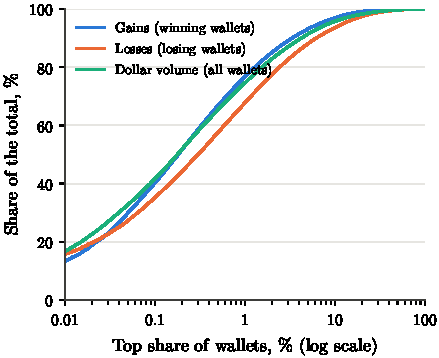
\includegraphics[width=0.55\textwidth]{figures/fig_wallets_lorenz.pdf}
\caption{Concentration of wallet outcomes: share of all gains (winning wallets), all losses (losing wallets) and all dollar volume held by the top $x$\% of wallets (equal shares would give $x$\%). Exact trade-based PnL over the sampled markets, net of fees.}\label{fig:wallets-lorenz}
\end{figure}

\begin{figure}[t]
\centering
% source: data/research/flb_wallets/persistence.csv, summary.json:persistence
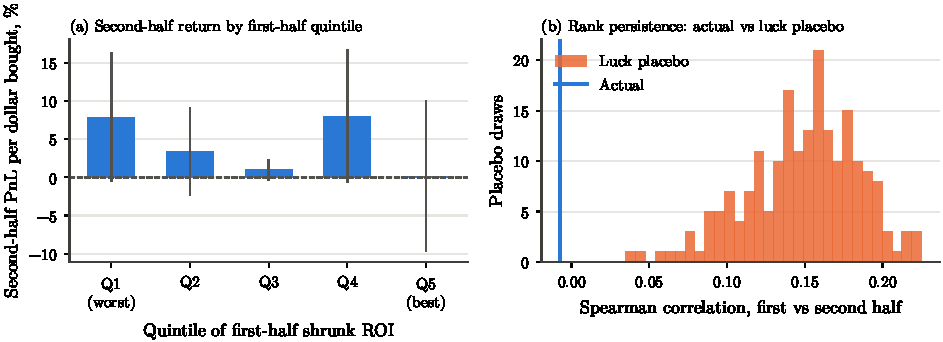
\includegraphics[width=\textwidth]{figures/fig_wallets_persist.pdf}
\caption{Persistence of wallet returns. (a) H2 PnL per dollar bought by quintile of shrunk H1 return, wallets active in both halves, with 95\% bootstrap intervals. (b) Rank correlation between halves under 200 draws of the luck placebo (outcomes redrawn from the last pre-information price) and the actual value on the same wallets.}\label{fig:wallets-persist}
\end{figure}

\begin{table}[t]
\centering
\small
\begin{threeparttable}
\caption{Profit concentration and persistence of wallet performance}\label{tab:wallets-skill}
% source: data/research/flb_wallets/summary.json:concentration, summary.json:persistence
\begin{tabular}{lr}
\toprule
\multicolumn{2}{l}{\emph{Concentration of PnL across wallets}} \\
Wallets in the sample & 237{,}569 \\
Share with positive PnL (\%) & 50.7 \\
Share of all gains: top 0.1\% / 1\% / 10\% of wallets (\%) & 51 / 85 / 99 \\
Wallets holding half of all gains / half of all losses & 220 / 326 \\
Gini: gains (winners) / losses (losers) / dollar volume & 0.97 / 0.95 / 0.96 \\
Leaderboard wallets: number / share of gains / share of volume (\%) & 96 / 11.8 / 10.4 \\
\addlinespace\multicolumn{2}{l}{\emph{Persistence, H1 $\to$ H2}} \\
Wallets active in both halves & 719 \\
Spearman, raw H1 ROI vs H2 ROI [95\% CI] & 0.02 [$-$0.06, 0.10] \\
Spearman, shrunk H1 ROI vs H2 ROI [95\% CI] & 0.02 [$-$0.06, 0.10] \\
Spearman, edge vs entry price, H1 vs H2 & $-$0.03 (694 wallets) \\
H2 ROI, top minus bottom quintile (\%, $t$) & $-$7.8 ($-$1.2) \\
Luck placebo: Spearman mean [5th, 95th pct.] & 0.15 [0.09, 0.20] \\
Actual Spearman on the placebo sample (percentile) & $-$0.01 (0) \\
Wallets with $\geq$20 markets: share with $t>2$, actual / placebo (\%) & 5.1 / 7.0 \\
\bottomrule
\end{tabular}
\begin{tablenotes}\footnotesize
\item PnL is exact trade-based PnL \eqref{eq:wallets-pnl} summed over the sampled markets, net of taker fees.
  Leaderboard: wallets on Polymarket's all-time overall, politics or sports top-100 (measured after the
  fact). Persistence: wallets with $\geq5$ markets and $\geq\$50$ bought in each half; shrunk ROI
  \eqref{eq:wallets-shrink}; edge = buy return minus its price bucket's mean in that half. The placebo redraws
  outcomes from the last pre-information price (200 draws). CIs from 500 wallet bootstraps.
\end{tablenotes}
\end{threeparttable}
\end{table}

\subsubsection{Retail inflows, attention and herding}\label{sec:res-wallets-dyn}

% source: data/research/flb_wallets/summary.json:dynamics, inflow_weekly.csv, inflow_events.csv, newwallet_monthly.csv, who_share.csv (dim=age_bucket)
Account creation dates are available for 5{,}144 wallets of the address-selected subset.
\Cref{fig:wallets-inflow}(a) plots their creation dates by week. The ratio of creations in the 14 days around each
event to the rate four to eight weeks before, with 95\% intervals, is: US election 2024 2.01 [1.64, 2.47]; Super Bowl LIX 0.40 [0.32, 0.49]; Papal conclave 2025 1.03 [0.76, 1.40]; NYC mayor 2025 2.59 [1.99, 3.37]; Super Bowl LX 1.26 [0.96, 1.65]. Each event window contains between 64 and
180 creations. Creations rise significantly around US election 2024 and NYC mayor 2025. They fall around Super Bowl LIX. That fall reflects its baseline. The four to eight weeks before Super Bowl LIX, mid-December to mid-January, are the peak of the inflow that began in the run-up to the 2024 election (\cref{fig:wallets-inflow}(a)).

New accounts put a smaller share of their buy fills into longshots. Longshots are 14.9\% of buy fills by accounts under a week old and
8.3\% at 7--30 days, against 19.9\% at 30--180 days and
22.7\% for older accounts (\cref{tab:wallets-sizeage}). In a fill-level linear probability model,
the difference between accounts under 30 days old and older accounts is $-$11.4 percentage points
($t=-3.3$, clustered by event). On a dollar basis the shares are 0.3\% and 0.8\%.
\Cref{fig:wallets-inflow}(b) shows the monthly shares. Attention-driven buying by new retail accounts,
documented for equities by \citet{barberodean2008} and \citet{barber2022}, would predict a higher share
for new accounts. The longshots that new accounts do buy, however, lose almost all of their cost:
$-$97.2\% ($t=-40.2$) per dollar for accounts under a week old and $-$88.3\% ($t=-12.1$) at
7--30 days, against 18.2\% ($t=0.2$) at 30--180 days and $-$31.3\% ($t=-0.5$) beyond
180 days.

% source: data/research/flb_wallets/summary.json:herding, herding.csv
Small retail buys cluster on one side. In one-hour windows with at least five small retail taker buys, the
\citet{lakonishok1992} measure \eqref{eq:wallets-lsv} is 0.095 ($t=20.9$;
23{,}823 windows). Independent orders would give zero. The clustering is not specific to retail:
taker buys by market-maker-like wallets cluster to the same degree (0.096, $t=9.4$;
536 windows). Same-side clustering within the hour is therefore a feature of order flow
around news, not of retail behaviour alone.

Retail herding moves prices only briefly. A window in which all small retail buys are on the YES side is
followed by a YES-price change of 0.16\cents{} ($t=3.4$) over the next hour, 0.09\cents{} ($t=0.7$) over six hours and $-$0.18\cents{} ($t=-0.5$) over 24
hours, controlling for the previous hour's change. The previous hour's change itself partly reverses (coefficient
$-$0.15, $t=-5.8$, at one hour). The same
imbalance does not predict the outcome relative to the price: the coefficient is $-$1.53\cents{} ($t=-1.2$). Small-wallet herding thus
neither carries information about outcomes nor leaves a reversal larger than the tick.

\begin{figure}[t]
\centering
% source: data/research/flb_wallets/inflow_weekly.csv, inflow_events.csv, newwallet_monthly.csv
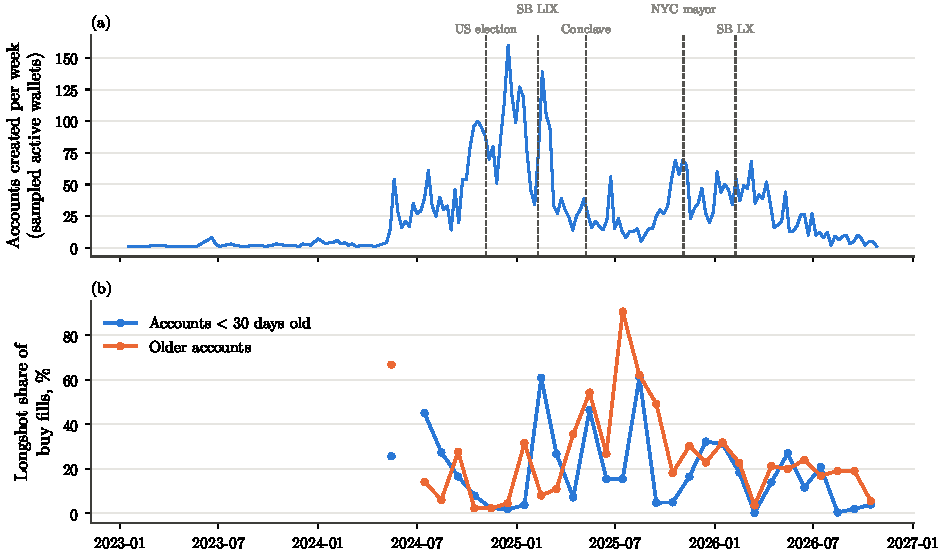
\includegraphics[width=\textwidth]{figures/fig_wallets_inflow.pdf}
\caption{Retail inflow and longshot buying. (a) Weekly account creations of the address-selected subset of sampled wallets, with five salient events marked. (b) Longshot share of design-weighted buy fills by accounts under 30 days old and by older accounts, by month (months with at least 30 fills), buy fills before the information time.}\label{fig:wallets-inflow}
\end{figure}

\subsubsection{The bias across venues}\label{sec:res-wallets-venues}

% source: data/research/flb_wallets/summary.json:xvenue, xvenue_gap.csv, xvenue_calib.csv
On 523 matched team-sides in 441 games, Kalshi and Polymarket agree almost exactly
before the start (\cref{tab:wallets-xvenue}, \cref{fig:wallets-xvenue}). One hour before the start the prices
correlate at 0.9993, and the mean absolute gap between the Polymarket price and the Kalshi midpoint is
0.40\cents. A day before it is 0.59\cents.

Game-winner markets rarely price a side at 10\cents{} or less an hour before the start: only 6
team-sides do, so the comparison cannot say whether one venue prices longshots higher. Between 11\cents{} and 80\cents{}
(495 team-sides), the mean gap in every bucket is within 0.05\cents{} of zero. Above 80\cents{}
(22 team-sides), Polymarket prices the favourite slightly below Kalshi's midpoint: by
0.59\cents{} at 90\cents{} or more
($t=-3.8$). Calibration slopes on the same team-sides are 0.71
for Kalshi and 0.71 for Polymarket ($t=-2.0$ and
$t=-2.0$ against one). The two are equal because the prices almost
coincide (\cref{tab:wallets-xvenue}). Gaps are short-lived:
\begin{itemize}
  \item the hour-to-hour autocorrelation of a pair's gap is 0.79, a half-life of about
    3.0 hours;
  \item the gap 24 hours out has a correlation of 0.09 with the gap an hour before the start.
\end{itemize}
Only 2.3\% of the one-hour gaps exceed the sum of the two venues' taker fees, and
0.2\% exceed fees plus Kalshi's half-spread. Within Polymarket,
\citet{saguillo2025} document arbitrage between related markets; across these two venues, price gaps on the
same games are almost always inside trading costs. We use no Polymarket US prices (\cref{sec:data-wallets}). By its
published schedule, a small Polymarket US account pays the highest taker fee of the three venues
(\cref{tab:wallets-fees}), so a gap involving that venue would have to be wider still to clear fees.

\begin{figure}[t]
\centering
% source: data/research/flb_wallets/xvenue_gap.csv
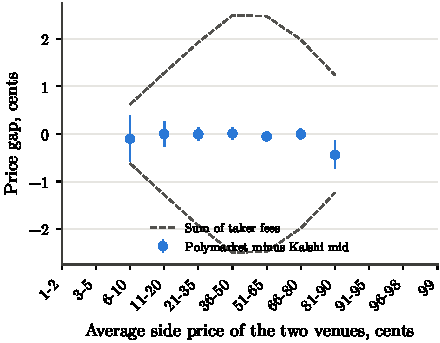
\includegraphics[width=0.55\textwidth]{figures/fig_wallets_xvenue.pdf}
\caption{Polymarket price minus Kalshi bid--ask midpoint for the same team, one hour before the scheduled start, by the two venues' average side price, with 95\% intervals clustered by game. Dashed: mean sum of the two venues' taker fees at those prices.}\label{fig:wallets-xvenue}
\end{figure}

\begin{table}[t]
\centering
\small
\begin{threeparttable}
\caption{Kalshi and Polymarket prices on the same games}\label{tab:wallets-xvenue}
% source: data/research/flb_wallets/summary.json:xvenue, xvenue_gap.csv, xvenue_calib.csv
\setlength{\tabcolsep}{4pt}
\begin{tabular}{rrrrrrrrrrrrr}
\toprule
Lead & Team & & Corr. & Mean $|g|$ & \multicolumn{2}{c}{$g$, $\bar q\le10\cents$} & \multicolumn{2}{c}{$g$, $\bar q\ge90\cents$} & \multicolumn{2}{c}{$|g|>$ fees (\%)} & \multicolumn{2}{c}{$\beta$} \\
\cmidrule(lr){6-7}\cmidrule(lr){8-9}\cmidrule(lr){10-11}\cmidrule(lr){12-13}
(h) & sides & Games & of prices & (\cents) & \cents & ($t$) & \cents & ($t$) & fees & +spread & Kalshi & PM \\
\midrule
1 & 523 & 441 & 0.9993 & 0.40 & $-$0.10 & ($-$0.5) & $-$0.59 & ($-$3.8) & 2.3 & 0.2 & 0.71 & 0.71 \\
3 & 523 & 441 & 0.9993 & 0.40 & $-$0.01 & ($-$0.0) & $-$0.04 & ($-$0.1) & 2.7 & 0.2 & 0.70 & 0.70 \\
6 & 523 & 441 & 0.9993 & 0.42 & $-$0.02 & ($-$0.1) & $-$0.12 & ($-$0.4) & 2.5 & 0.0 & 0.70 & 0.69 \\
12 & 523 & 441 & 0.9967 & 0.54 & $+$0.31 & (0.9) & $+$0.19 & (0.6) & 3.8 & 1.1 & 0.69 & 0.69 \\
24 & 514 & 432 & 0.9976 & 0.59 & $-$0.19 & ($-$0.4) & $+$0.23 & (0.6) & 4.9 & 0.6 & 0.69 & 0.69 \\
\bottomrule
\end{tabular}
\begin{tablenotes}\footnotesize
\item Kalshi NBA, NHL, NFL, college-football and WNBA game-winner markets (August--October 2026) matched to the
  same team's Polymarket outcome, observed on the same hourly timestamp $L$ hours before the scheduled
  start. $g=p^{\mathrm{PM}}-p^{\mathrm{K}}$ with $p^{\mathrm{K}}$ the Kalshi bid--ask midpoint; $\bar q$ is the two venues'
  average price of that side. Fees: Kalshi taker $0.07\,p(1-p)$ plus each Polymarket market's taker rate;
  ``+spread'' adds Kalshi's half-spread. $\beta$: calibration slope \eqref{eq:logit} on the same team-sides.
  $t$-statistics clustered by game.
\end{tablenotes}
\end{threeparttable}
\end{table}

\paragraph{Summary.}
On identified Polymarket wallets, the pattern predicted by \cref{hyp:pref} appears in who trades longshots, not
in who profits:
\begin{itemize}
  \item longshots are a large share of the buying of small wallets and market makers, and almost none of the
    buying of whales and mid-size wallets;
  \item small, occasional wallets are significant net buyers of longshots, and their buying is absorbed by
    all other classes, none of which is individually a significant net seller;
  \item new accounts put a smaller share of their buying into longshots than established ones, but lose
    almost all of what they put in;
  \item longshot buys lose about half their cost on average and favourite buys earn a few per cent;
  \item wallet profits are extremely concentrated, but they do not persist out of sample;
  \item Kalshi and Polymarket price the same games almost identically.
\end{itemize}

\subsection{What explains the bias}\label{sec:res-structural}
% Workstream structural: results. Numbers are macros from the AUTO block of method_structural.tex;
% tables are generated by `python -m albert.research.flb_structural run latex` (data/research/flb_structural/).

We ask how much of the longshot overpricing each explanation of \cref{sec:framework} accounts for, using the
methods of \cref{sec:method-structural}. The sample is the final panel of \cref{sec:res-xs}: \sdQuotes{} pre-event
quotes on \sdMarkets{} markets in \sdEvents{} events, with \sdLsSides{} longshot side observations. Quantities are
in cents per contract at the calibration level, because pooled returns per dollar on longshots rest on a few large
wins (\cref{sec:res-flow}). Supporting tables and figures are in \cref{app:structural}.

\subsubsection{Mechanical frictions}\label{sec:res-structural-band}

\Cref{tab:structural-band,fig:structural-band} decompose the longshot gap as in~\eqref{eq:structural-decomp}.
\begin{itemize}
  \item \emph{Size of the gap.} Longshot sides cost \sdLsPrice\cents{} at the mid and win \sdLsWin\% of the time,
  a gap of \sdLsGross\cents{} per contract ($t=\sdLsGrossT$).
  \item \emph{Cost of selling as a taker.} It is \sdLsBand\cents:
  \begin{itemize}
    \item \sdLsFloor{} of half-spread at the tick floor;
    \item \sdLsSpread{} of other half-spread;
    \item \sdLsFee{} of fees;
    \item \sdLsCap{} of capital at 5\% a year.
  \end{itemize}
  \item \emph{Residual.} It is $\bar R=\sdLsResid\cents$ ($t=\sdLsResidT$). Market-weighted, the mispricing lies
  inside the taker band in every price bucket, as in \cref{tab:xs-limits}. In no group is the residual
  significantly positive.
  \item \emph{Sides with a bid.} Where a taker sale is possible at all, the residual is \sdRobBidResid\cents{}
  ($t=\sdRobBidResidT$). This is the per-contract counterpart of taking the other side of longshots in
  \cref{tab:xs-limits}.
  \item \emph{Short leads.} At leads of a day or less, the gap sits at the edge of the band (residuals of
  \sdLeadOneHResid, \sdLeadSixHResid{} and \sdLeadOneDResid\cents).
\end{itemize}

Frictions thus explain why takers do not trade the bias away, but not where it comes from.
\begin{enumerate}
  \item \emph{The floor explains the cheapest bucket only.} The floor's half-spread is \sdBOneFloorShare\% of the
  1--2\cents{} gap. \Cref{tab:xs-limits} finds less because it counts the realised loss of floor quotes. Across all
  longshots, the floor is \sdLsFloorShare\% of the gap. On the 0.1\cents{} grid, whose floor is ten times lower
  (\sdSubCentBN{} sides, \sdSubCentBClusters{} events), the 1--2\cents{} gap is \sdSubCentBGross\cents{}, against
  \sdOneCentBGross\cents{} on the 1\cents{} grid, with a residual of \sdSubCentBResid\cents{} ($t=\sdSubCentBResidT$).
  \item \emph{The bias does not grow with the horizon.} Capital costs at most \sdLeadThirtyDCap\cents{} at 30 days.
  Within price buckets, the gap \emph{falls} by \sdHzGross\cents{} per unit of log lead ($t=\sdHzGrossT$), and the
  residual by \sdHzResid{} ($t=\sdHzResidT$). The raw gap is larger at 30 days (\sdLeadThirtyDGross{} against
  \sdLeadOneHGross\cents) because longshots quoted that far ahead are dearer (\sdLeadThirtyDPrice{} against
  \sdLeadOneHPrice\cents{} at the mid). \Cref{hyp:mech} and \citet{pageclemen2013}
  predict growth with the horizon.
  \item \emph{The cost of capital is immaterial.} The residual is \sdRhoZeroResid\cents{} at $\rho=0$ and
  \sdRhoTenResid\cents{} at $\rho=10\%$.
  \item \emph{Where the volume is, the bias exceeds the band.} Volume-weighted, the gap is \sdLsVolGross\cents{}
  but the band only \sdLsVolBand\cents, because active markets have tight spreads. The residual is
  \sdLsVolResid\cents{} ($t=\sdLsVolResidT$).
  \item \emph{Makers could earn the gap.} Selling at the ask would earn $\bar R^{mk}=\sdLsResidMk\cents$
  ($t=\sdLsResidMkT$). This is an upper bound that ignores adverse selection, consistent with \cref{sec:res-flow}.
\end{enumerate}

\begin{figure}[!htbp]
\centering
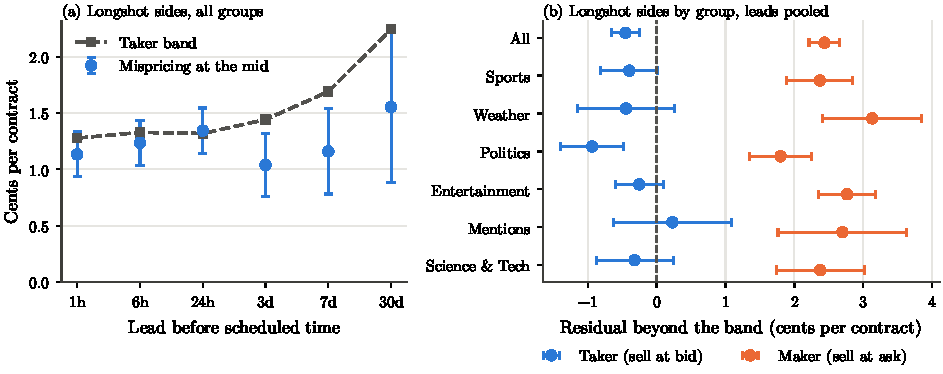
\includegraphics[width=\textwidth]{figures/fig_structural_band.pdf}
\caption{The longshot mispricing and the no-arbitrage band. Left: price at the mid minus realised win rate of
longshot sides ($\q\le10\cents$) by lead, against the taker band (tick floor, half-spread, fee and capital at
$\rho=5\%$). Right: the residual beyond the band, the mean profit per contract of selling longshots at the bid
(taker) or at the ask (maker, an upper bound), by group with leads pooled. Market-weighted; 95\% confidence
intervals clustered by event.}\label{fig:structural-band}
\end{figure}

% BEGIN AUTO:tab-band
\begin{table}[!htbp]
\centering
\begin{threeparttable}
\caption{Longshot mispricing and the no-arbitrage band}\label{tab:structural-band}
\scriptsize
\setlength{\tabcolsep}{3pt}
\begin{tabular}{@{}lrrrrrrrrrrr@{}}
\toprule
 & & & & Gross & \multicolumn{4}{c}{Band components} & Residual & Maker & In band \\
\cmidrule(lr){6-9}
Cell & Sides & Events & $\bar\q$ & $\bar\q-\bar\won$ & Floor & Half-spr. & Fee & Capital & $\bar R$ & $\bar R^{mk}$ & (\%) \\
\midrule
% source: data/research/flb_structural/band_cells.csv
All longshots & 40{,}552 & 3{,}091 & 2.54 & 1.07 (10.0) & 0.18 & 1.23 & 0.07 & 0.04 & $-$0.45 ($-$4.3) & 2.44 (21.3) & 100 \\
\multicolumn{12}{@{}l}{\emph{By lead, all groups}} \\
\quad 1h & 9{,}847 & 2{,}690 & 2.05 & 1.13 (11.2) & 0.23 & 0.99 & 0.05 & 0.00 & $-$0.14 ($-$1.5) & 2.35 (21.7) & 100 \\
\quad 6h & 9{,}721 & 2{,}633 & 2.17 & 1.24 (12.2) & 0.21 & 1.06 & 0.06 & 0.00 & $-$0.09 ($-$0.9) & 2.49 (23.1) & 100 \\
\quad 24h & 8{,}025 & 1{,}962 & 2.10 & 1.34 (13.1) & 0.20 & 1.04 & 0.06 & 0.01 & 0.03 (0.3) & 2.57 (22.9) & 98 \\
\quad 3d & 7{,}056 & 1{,}742 & 2.44 & 1.04 (7.3) & 0.17 & 1.16 & 0.07 & 0.04 & $-$0.40 ($-$2.9) & 2.32 (15.1) & 100 \\
\quad 7d & 4{,}149 & 1{,}180 & 2.56 & 1.16 (6.0) & 0.15 & 1.38 & 0.07 & 0.09 & $-$0.53 ($-$2.8) & 2.59 (12.5) & 100 \\
\quad 30d & 1{,}754 & 670 & 3.38 & 1.55 (4.5) & 0.09 & 1.64 & 0.11 & 0.40 & $-$0.69 ($-$2.0) & 2.89 (8.0) & 100 \\
\multicolumn{12}{@{}l}{\emph{By group, leads pooled}} \\
\quad Sports & 9{,}108 & 502 & 2.29 & 1.07 (4.9) & 0.22 & 1.14 & 0.06 & 0.04 & $-$0.40 ($-$1.9) & 2.37 (9.7) & 100 \\
\quad Weather & 3{,}905 & 721 & 3.46 & 1.42 (4.0) & 0.11 & 1.62 & 0.12 & 0.02 & $-$0.44 ($-$1.2) & 3.13 (8.6) & 100 \\
\quad Politics & 11{,}768 & 835 & 2.51 & 0.51 (2.2) & 0.15 & 1.17 & 0.08 & 0.04 & $-$0.94 ($-$4.0) & 1.80 (7.8) & 100 \\
\quad Entertainment & 8{,}939 & 494 & 2.22 & 1.31 (7.1) & 0.19 & 1.30 & 0.05 & 0.03 & $-$0.25 ($-$1.4) & 2.76 (13.2) & 100 \\
\quad Mentions & 1{,}918 & 91 & 3.22 & 1.55 (3.5) & 0.20 & 0.96 & 0.14 & 0.02 & 0.23 (0.5) & 2.70 (5.7) & 85 \\
\quad Science \& Tech & 4{,}572 & 401 & 2.30 & 1.12 (3.8) & 0.18 & 1.14 & 0.07 & 0.05 & $-$0.32 ($-$1.1) & 2.37 (7.3) & 100 \\
\bottomrule
\end{tabular}
\begin{tablenotes}\footnotesize
\item Side observations with $\q\le10\cents$ at the mid, pre-event quotes. All entries in cents per contract. Gross: price at the mid minus the realised win rate. The band components (\cref{eq:structural-decomp}) are the half-spread of sides pinned at the tick floor (Floor), the half-spread of other sides, the taker fee and the capital cost at $\rho=5\%$ a year over the lead. $\bar R$: residual beyond the taker band, the mean net profit per contract of selling the side at its bid; $\bar R^{mk}$: selling at its ask as a maker (an upper bound: no adverse selection). In band: share of the gross mispricing the taker band covers, $\min(\text{band},\text{gross})/\text{gross}$. Market-weighted (each market once per cell; within a lead, equal weights). Cells by price bucket and structure are in \cref{tab:structural-band-groups,tab:structural-band-robust}; the band per bucket agrees with \cref{tab:xs-limits}. $t$-statistics clustered by event in parentheses.
\end{tablenotes}
\end{threeparttable}
\end{table}
% END AUTO:tab-band

\subsubsection{Probability weighting}\label{sec:res-structural-weighting}

In \cref{tab:structural-weighting}, the LLO curvature is $\gamma=1/\beta$ for the slope $\beta$ of
\cref{tab:xs-group}, estimated on the identical sample.
\begin{itemize}
  \item \emph{Pooled.} $\gamma=\sdAllGamma$ (standard error \sdAllGammaSe; $t_{\gamma<1}=\sdAllGammaT$), and the
  Prelec curvature is also \sdAllPrGamma. Both overweight small probabilities, with near-neutral elevation
  ($\delta=\sdAllDelta$ and \sdAllPrDelta).
  \item \emph{Groups.} $\gamma$ is below one in \sdGammaBelowOne{} of \sdNGroups{} groups (\sdGammaMin--\sdGammaMax).
  A common $\gamma$ is not rejected market-weighted ($p=\sdWaldGroupP$). It is rejected volume-weighted
  ($p=\sdWaldGroupVolP$), where the distortion is stronger ($\gamma=\sdAllVolGamma$).
  \item \emph{Leads and halves.} Across leads $\gamma$ ranges from \sdLeadGammaMin{} to \sdLeadGammaMax{}
  ($p=\sdWaldLeadP$). It is \sdHalfFirstGamma{} and \sdHalfSecondGamma{} in the two halves.
  \item \emph{Out of sample.} Fitted on one half of the months and scored on the other, pooled LLO improves the log
  score of face-value prices by only \sdOosFsLlo{} ($t=\sdOosFsLloT$) and \sdOosSfLlo{} milli-nats per quote, and
  Prelec by \sdOosFsPrelec{} and \sdOosSfPrelec. The log loss itself is \sdOosFsCalLs{} nats. A constant YES shift
  lowers the score (\sdOosFsShift, $t=\sdOosFsShiftT$). Group-specific LLO is worse than pooled LLO by
  \sdOosFsGroupVsPooled{} ($t=\sdOosFsGroupVsPooledT$) and \sdOosSfGroupVsPooled{} ($t=\sdOosSfGroupVsPooledT$).
\end{itemize}
One mild inverse-S function thus describes all categories. It is precisely estimated but small next to the
information in prices.

% BEGIN AUTO:tab-weighting
\begin{table}[!htbp]
\centering
\begin{threeparttable}
\caption{Probability weighting: fitted functions, equality tests and forecasts}\label{tab:structural-weighting}
\scriptsize
\setlength{\tabcolsep}{3.5pt}
\begin{tabular}{@{}lrrrrrrrrr@{}}
\toprule
 & & & \multicolumn{3}{c}{LLO} & \multicolumn{2}{c}{Prelec} & \multicolumn{2}{c}{$\Delta\log L$} \\
\cmidrule(lr){4-6}\cmidrule(lr){7-8}\cmidrule(l){9-10}
Group & Quotes & Events & $\gamma$ & $\delta$ & $t_{\gamma<1}$ & $\gamma$ & $\delta$ & LLO & Prelec \\
\midrule
% source: data/research/flb_structural/weighting_fits.csv, weighting_insample.csv, weighting_oos.csv, summary.json:weighting.wald
\multicolumn{10}{@{}l}{\emph{Panel A. Fitted weighting functions}} \\
All groups & 61{,}992 & 4{,}770 & 0.89 (0.016) & $-$0.06 (0.029) & 7.4 & 0.89 (0.016) & 1.01 (0.016) & 1.4 & 1.6 \\
Sports & 18{,}303 & 1{,}521 & 0.91 (0.031) & $-$0.04 (0.047) & 2.9 & 0.90 (0.027) & 1.00 (0.027) & 0.8 & 1.2 \\
Weather & 6{,}796 & 1{,}065 & 0.87 (0.040) & $-$0.10 (0.047) & 3.3 & 0.89 (0.039) & 1.02 (0.022) & 1.6 & 1.6 \\
Politics & 15{,}774 & 968 & 0.93 (0.036) & $-$0.07 (0.065) & 1.9 & 0.93 (0.035) & 1.03 (0.032) & 0.4 & 0.5 \\
Entertainment & 10{,}424 & 530 & 0.80 (0.034) & 0.04 (0.076) & 6.0 & 0.85 (0.035) & 0.97 (0.041) & 5.1 & 5.0 \\
Mentions & 4{,}743 & 103 & 0.89 (0.049) & $-$0.03 (0.106) & 2.3 & 0.88 (0.052) & 0.99 (0.060) & 1.5 & 2.0 \\
Science \& Tech & 5{,}472 & 510 & 0.85 (0.049) & $-$0.17 (0.141) & 3.0 & 0.84 (0.052) & 1.08 (0.083) & 3.2 & 3.6 \\
\midrule
\multicolumn{10}{@{}l}{\emph{Panel B. Equal slopes ($\gamma$) across cells: Wald tests}} \\
\multicolumn{3}{@{}l}{Groups} & \multicolumn{7}{l}{$\chi^2_{5}=8.6$, $p=0.127$, 4{,}697 events} \\
\multicolumn{3}{@{}l}{Groups, $\gamma$ and $\delta$} & \multicolumn{7}{l}{$\chi^2_{10}=16.6$, $p=0.084$, 4{,}697 events} \\
\multicolumn{3}{@{}l}{Structures} & \multicolumn{7}{l}{$\chi^2_{3}=7.5$, $p=0.057$, 4{,}770 events} \\
\multicolumn{3}{@{}l}{Leads} & \multicolumn{7}{l}{$\chi^2_{5}=12.1$, $p=0.033$, 4{,}770 events} \\
\multicolumn{3}{@{}l}{Groups, volume-weighted} & \multicolumn{7}{l}{$\chi^2_{5}=12.8$, $p=0.026$, 4{,}357 events} \\
\midrule
\multicolumn{10}{@{}l}{\emph{Panel C. Out-of-sample log score against calibrated prices (milli-nats per quote)}} \\
\multicolumn{3}{@{}l}{Constant shift} & \multicolumn{7}{l}{first $\to$ second half: $-$1.32 ($-$2.9); second $\to$ first: $-$0.73 ($-$4.4)} \\
\multicolumn{3}{@{}l}{LLO, pooled} & \multicolumn{7}{l}{first $\to$ second half: 0.46 (0.9); second $\to$ first: 0.04 (0.1)} \\
\multicolumn{3}{@{}l}{Prelec, pooled} & \multicolumn{7}{l}{first $\to$ second half: 0.75 (1.7); second $\to$ first: 0.19 (0.3)} \\
\multicolumn{3}{@{}l}{LLO, by group} & \multicolumn{7}{l}{first $\to$ second half: $-$2.65 ($-$2.3); second $\to$ first: $-$1.79 ($-$1.6)} \\
\bottomrule
\end{tabular}
\begin{tablenotes}\footnotesize
\item YES sides of pre-event quotes, market-weighted. LLO: $\operatorname{logit}\q=\delta+\gamma\operatorname{logit}\pi$, estimated as~\eqref{eq:logit} with $\gamma=1/\beta$ and $\delta=-\alpha/\beta$. Prelec: $\q=\exp(-\delta(-\ln\pi)^\gamma)$. Maximum likelihood on outcomes; standard errors in parentheses clustered by event (delta method for $\gamma$, $\delta$). $\Delta\log L$: in-sample gain in mean log likelihood over calibrated prices, milli-nats per market. Panel B: cluster-robust Wald tests from one fully interacted logit. Panel C: models fitted on one half of the months and scored on the other; differences against $\Prob(y=1)=\q$ with event-clustered $t$ in parentheses.
\end{tablenotes}
\end{threeparttable}
\end{table}
% END AUTO:tab-weighting

\subsubsection{Insiders}\label{sec:res-structural-shin}

\Cref{tab:structural-shin} extends \cref{tab:xs-multi} to two-leg events and partition ladders, by group and
lead. Of \sdShinAllEventLeads{} event-leads, \sdShinIncomplete{} miss a quote on some leg and \sdShinNotOneYes{} lack
exactly one winner. That leaves \sdShinEventLeads{} on \sdShinUnits{} events. The asks sum to less than one in
\sdShinAskBelow{} of them and the mids in \sdShinMidBelow. Mentions events are not partitions.
\begin{itemize}
  \item \emph{The overround restates the spread.} $\shinz$ from the asks averages \sdShinAllZask, and from the mids
  \sdShinAllZmid. It rises by \sdZregSpread{} per cent of half-spread ($t=\sdZregSpreadT$; $R^2=\sdZregRsq$ with leg
  count). Given the spread, it is higher in the information groups by \sdZregInfo{} ($t=\sdZregInfoT$), small
  against its mean of \sdShinAllZask.
  \item \emph{The shading the outcomes require.} Fitted to outcomes, $\hat\shinz=\sdShinAllZml$
  [\sdShinAllZmlLo, \sdShinAllZmlHi], more than twice the margin's $\shinz$. It is \sdZmlInfo{} in the information
  groups and \sdZmlPublic{} in Sports and Weather (difference \sdZmlDiff, [\sdZmlDiffLo, \sdZmlDiffHi]). Politics
  needs the least of any group (\sdShinPoliticsZml).
  \item \emph{Forecasts} (\cref{tab:structural-shin-forecasts}). Longshot legs are overpriced by \sdLsAllMid\cents{}
  at the mid ($t=\sdLsAllMidT$), \sdLsAllNorm{} after normalisation and \sdLsAllShinAsk{} after Shin's correction from
  the asks. Shin beats the normalised asks by \sdScAllShinAsk{} milli-nats per leg ($t=\sdScAllShinAskT$), as
  \citet{strumbelj2014} found for bookmakers, but it does so by undoing the spread. A $\shinz$ fitted on the first
  half shrinks the second-half gap from \sdLsTestMid{} to \sdLsTestShinFit\cents{} ($t=\sdLsTestShinFitT$), acting
  as a calibration curve like LLO.
  \item \emph{Overpricing and $\shinz$.} Longshot overpricing rises with an event's $\shinz$ from the asks
  (\sdLsOnZ{} cents per unit, $t=\sdLsOnZT$). Since that $\shinz$ mostly measures the spread, the band predicts the
  same.
\end{itemize}

% BEGIN AUTO:tab-shin
\begin{table}[!htbp]
\centering
\begin{threeparttable}
\caption{Shin's insider share in events whose legs partition the outcomes}\label{tab:structural-shin}
\scriptsize
\setlength{\tabcolsep}{2.8pt}
\begin{tabular}{@{}lrrrrrrrr@{}}
\toprule
 & Event- & & Legs & $\sum a-1$ & $\sum p-1$ & $\shinz$ from & $\shinz$ from & $\shinz$ fitted \\
Sample & leads & Events & (med.) & (\%) & (\%) & asks & mids & to outcomes [95\% CI] \\
\midrule
% source: data/research/flb_structural/shin_cells.csv, summary.json:shin.info_vs_public
All partition events & 3{,}955 & 1{,}421 & 2 & 7.8 (33.0) & 1.3 (12.8) & 0.030 (0.0005) & 0.004 & 0.080 [0.020, 0.130] \\
\quad Two-leg events & 2{,}009 & 740 & 2 & 3.0 (40.6) & $-$0.2 ($-$4.0) & 0.032 (0.0008) & 0.003 & 0.025 [0.005, 0.095] \\
\quad Multi-outcome events & 1{,}289 & 381 & 4 & 10.1 (17.1) & 2.2 (7.6) & 0.026 (0.0008) & 0.005 & 0.095 [0.025, 0.245] \\
\quad Partition ladders & 657 & 300 & 9 & 16.7 (38.3) & 3.9 (16.3) & 0.030 (0.0008) & 0.008 & 0.105 [0.005, 0.225] \\
\quad Sports & 2{,}373 & 916 & 2 & 4.7 (20.7) & 0.3 (2.6) & 0.030 (0.0007) & 0.003 & 0.060 [0.020, 0.125] \\
\quad Weather & 237 & 139 & 6 & 15.5 (25.5) & 4.1 (11.4) & 0.034 (0.0014) & 0.010 & 0.110 [0.020, 0.420] \\
\quad Politics & 1{,}011 & 280 & 6 & 12.6 (23.3) & 2.6 (12.3) & 0.028 (0.0008) & 0.005 & 0.025 [0.005, 0.165] \\
\quad Entertainment & 120 & 42 & 8 & 17.9 (8.2) & 6.3 (5.8) & 0.036 (0.0034) & 0.010 & 0.070 [0.005, 0.230] \\
\quad Science \& Tech & 214 & 44 & 7 & 7.6 (5.4) & 1.8 (2.3) & 0.018 (0.0019) & 0.005 & 0.195 [0.090, 0.600] \\
\quad Information minus public & & & & & & $-$0.003 & & 0.015 [$-$0.110, 0.090] \\
\bottomrule
\end{tabular}
\begin{tablenotes}\footnotesize
\item Mutually exclusive events (Kalshi flag) and strike ladders that partition the outcome space, at leads where every leg has a usable quote and exactly one leg settles YES. $a$, $p$: YES ask and mid. $\shinz$ from asks or mids solves~\eqref{eq:shin} ($\shinz=0$ when the prices sum to at most one). Fitted $\shinz$: the value on a grid over $[0,0.6]$ that maximises the log score of the winning leg, with the scale chosen so that probabilities sum to one; 95\% event-bootstrap interval. Each event weighs one across its leads; \cref{tab:xs-multi} weights event-leads equally, hence the small differences in the multi-outcome row. Information groups: Politics, Entertainment, Mentions, Science \& Tech; public: Sports, Weather. Standard errors (of $\shinz$) or $t$-statistics (of the overrounds) clustered by event in parentheses.
\end{tablenotes}
\end{threeparttable}
\end{table}
% END AUTO:tab-shin

\subsubsection{Belief dispersion}\label{sec:res-structural-beliefs}

The slope interactions of~\eqref{eq:structural-interact} are in \cref{tab:structural-beliefs,fig:structural-beliefs}.
\begin{itemize}
  \item \emph{Number of outcomes.} More outcomes steepen the slope by \sdPoolLogOutcomes{} per standard deviation
  ($t=\sdPoolLogOutcomesT$; within groups \sdWithinLogOutcomes, $t=\sdWithinLogOutcomesT$). This is the sign
  \cref{hyp:beliefs} predicts, but not significant.
  \item \emph{Turnover.} Turnover flattens the slope (\sdPoolTurnover, $t=\sdPoolTurnoverT$). The interaction is
  positive in only \sdSignTurnoverPos{} of \sdSignTurnoverOf{} groups.
  \item \emph{Forecast anchor.} The anchor interaction is \sdPoolAnchored{} ($t=\sdPoolAnchoredT$), and it flips
  sign between halves (\sdHalfFirstAnchored{} and \sdHalfSecondAnchored).
  \item \emph{Horizon and spread.} Longer horizons flatten the slope (\sdPoolLogLead, $t=\sdPoolLogLeadT$). Wider
  spreads leave the slope unchanged but raise the longshot gap in cents (\sdLsWSpreadC, $t=\sdLsWSpreadCT$), as the
  band predicts.
\end{itemize}

\subsubsection{Synthesis}\label{sec:res-structural-synthesis}

\Cref{tab:structural-scorecard-groups} summarises the evidence by group; \cref{tab:structural-scorecard} lists every
prediction tested.

% BEGIN AUTO:tab-scorecard-groups
\begin{table}[!htbp]
\centering
\begin{threeparttable}
\caption{The evidence by group}\label{tab:structural-scorecard-groups}
\scriptsize
\setlength{\tabcolsep}{3.5pt}
\begin{tabular}{@{}lrrrrr@{}}
\toprule
 & \multicolumn{2}{c}{\Cref{hyp:mech}: band} & \Cref{hyp:pref}: weighting & \Cref{hyp:info}: insiders & \Cref{hyp:beliefs}: dispersion \\
\cmidrule(lr){2-3}
Group & Residual $\bar R$ (\cents) & In band (\%) & $\gamma$ ($t_{\gamma<1}$) & fitted $\shinz$ [95\% CI] & Turnover \\
\midrule
% source: data/research/flb_structural/scorecard.csv
All groups & $+$ $-$0.45 ($-$4.3) & 100 & $+$ 0.89 (7.4) &  0.080 [0.02, 0.13] & $0$ $-$0.043 ($-$1.5) \\
Sports & $+$ $-$0.40 ($-$1.9) & 100 & $+$ 0.91 (2.9) & $-$ 0.060 [0.02, 0.12] & $0$ 0.025 (0.6) \\
Weather & $+$ $-$0.44 ($-$1.2) & 100 & $+$ 0.87 (3.3) & $-$ 0.110 [0.02, 0.42] & $0$ $-$0.054 ($-$0.4) \\
Politics & $+$ $-$0.94 ($-$4.0) & 100 & $0$ 0.93 (1.9) & $+$ 0.025 [0.01, 0.17] & $-$ $-$0.127 ($-$2.7) \\
Entertainment & $+$ $-$0.25 ($-$1.4) & 100 & $+$ 0.80 (6.0) & $+$ 0.070 [0.01, 0.23] & $0$ $-$0.101 ($-$1.8) \\
Mentions & $+$ 0.23 (0.5) & 85 & $+$ 0.89 (2.3) & -- & $0$ $-$0.107 ($-$1.7) \\
Science \& Tech & $+$ $-$0.32 ($-$1.1) & 100 & $+$ 0.85 (3.0) & $+$ 0.195 [0.09, 0.60] & $0$ $-$0.088 ($-$1.3) \\
\bottomrule
\end{tabular}
\begin{tablenotes}\footnotesize
\item Mark: $+$ consistent with the hypothesis's prediction for the group, $-$ inconsistent, $0$ inconclusive. \Cref{hyp:mech}: $+$ when the longshot residual beyond the taker band is not significantly positive. \Cref{hyp:pref}: $+$ when $\gamma<1$ significantly. \Cref{hyp:info}: in Politics, Entertainment, Mentions and Science \& Tech $+$ when the interval for the fitted $\shinz$ excludes zero; in Sports and Weather, where outcomes are public, $+$ when it includes zero and $-$ when it does not. \Cref{hyp:beliefs}: sign and significance of the turnover interaction (within-group slopes for all groups). Sources and clustering as in \cref{tab:structural-band,tab:structural-weighting,tab:structural-shin,tab:structural-beliefs}.
\end{tablenotes}
\end{threeparttable}
\end{table}
% END AUTO:tab-scorecard-groups

\Cref{tab:structural-decomp} applies each explanation's map from prices to probabilities to the second-half
longshot gap of \sdCfGross\cents.
\begin{itemize}
  \item The taker band covers \sdCfBandShare\% of the gap.
  \item LLO fitted on the first half removes \sdCfLloShare\% (residual \sdCfLloResid\cents, $t=\sdCfLloResidT$).
  Prelec removes \sdCfPrelecShare\%, and group-specific LLO \sdCfLloGroupShare\%.
  \item In partition events, normalisation removes \sdCfNormShare\%, Shin with the margin's $\shinz$
  \sdCfShinAskShare\%, and Shin with a fitted $\shinz$ \sdCfShinFitShare\%.
\end{itemize}
The shares are not additive. The band measures what frictions \emph{allow}; the fitted maps measure what a
calibration curve \emph{describes}.

Prices and outcomes cannot separate four things:
\begin{itemize}
  \item risk-love from probability weighting, which needs bet sizes or exotic bets \citep{snowbergwolfers2010};
  \item weighting from heterogeneous beliefs, since both yield a monotone calibration curve that LLO fits by
  construction \citep{gandhi2015,manski2006};
  \item insiders from the spread, which itself prices informed trading \citep{glostenmilgrom1985};
  \item the true cost of capital.
\end{itemize}
We therefore report no variance decomposition.

\paragraph{Summary of verdicts.}
\begin{enumerate}
  \item \emph{Mechanical (\cref{hyp:mech}): \sdVerdictOne{} (\sdPassedOne{} predictions hold).} Spreads, fees and
  the tick floor explain why the bias survives: market-weighted, it is no larger than the cost of selling it as a
  taker in any group. They do not explain where it comes from. It falls rather than grows with the horizon, a
  finer tick does not remove it, and volume-weighted it exceeds the band.
  \item \emph{Preference (\cref{hyp:pref}): \sdVerdictTwo{} (\sdPassedTwo).} Prices behave as if traders weight
  probabilities with one mild inverse-S function, $\gamma\approx\sdAllGamma$, below one in every category, though it
  adds little out of sample. Small takers and retail wallets buy the longshots and lose
  (\cref{sec:res-flow,sec:res-wallets}). Together, this makes preference the best-supported explanation.
  \item \emph{Information (\cref{hyp:info}): \sdVerdictThree{} (\sdPassedThree).} The predictions that hold are
  small and confounded with the spread. The margin's shading removes none of the longshot overpricing. The shading
  the outcomes require is not larger where private information is plausible, and it is smallest in Politics.
  \item \emph{Belief dispersion (\cref{hyp:beliefs}): \sdVerdictFour{} (\sdPassedFour).} The bias is not
  significantly steeper with more outcomes or turnover, and anchors do not reliably flatten it.
\end{enumerate}



\section{Discussion}\label{sec:discussion}
% Discussion. Numbers are quoted from the results sections; sources are given there.
\subsection{What the three data sets agree on}

The three samples measure the bias in different ways. The quote panel uses mid-quotes at fixed
leads. The Kalshi trade sample uses the prices at which orders executed. The Polymarket sample uses
fills by identified wallets. They agree on four points.
\begin{itemize}
  \item \emph{Longshots lose and favourites roughly break even.} On Kalshi, longshot sides return
  $-55\%$ per dollar at the mid. On Polymarket, longshot buys return $-54\%$ per dollar. In
  Kalshi's trade sample, taker longshot positions lose in 14 of 18 strata. Favourites earn between
  zero and a few per cent on both venues.
  \item \emph{The bias is small per contract.} In probability units the mispricing is a fraction
  of a cent to a few cents (\cref{sec:res-xs-limits}). Per dollar it is large only because the
  price is small. Sides quoted at 3--5\cents{} return $-54\%$ per dollar at the mid, so they win
  about half as often as their price implies, yet the absolute error is only about two cents.
  \item \emph{Small traders hold the longshots.} On both venues, longshots are a large share of
  small orders or small wallets and almost none of large orders or whales.
  \item \emph{Nobody is reliably on the other side.} Kalshi makers earn little more than takers
  overall, and on Polymarket no class of wallets is a significant net seller of longshots. The
  wallets that profit do not persist.
\end{itemize}
They differ in one respect. Polymarket's market-level calibration slope a day ahead, $0.99$
(SE $0.15$), is imprecise and cannot be distinguished from Kalshi's $1.13$, but the equal-weight
estimate, $0.97$ (SE $0.05$), is lower. Polymarket trades on a sub-cent grid near the extremes (89\% of
its fills below 4\cents{} or above 96\cents{} are at sub-cent prices)
% source: data/research/flb_lead/checks.json
and charged no fees for most of the sample, so both mechanical frictions of \cref{sec:framework} were
weaker there. The samples, price measures and periods also differ, so we do not read the gap as a
venue effect. On the 441 games observed on both venues, prices are almost identical.

\subsection{Interpreting the bias}

\paragraph{Mechanics set the band, not the position within it.} The one-cent tick and the fee
schedule explain why the bias cannot be traded away. A contract worth a tenth of a cent cannot be
quoted below a cent, and a taker who sells the longshot pays a spread and a fee that absorb the
whole premium. This is a limit to arbitrage in the sense of \citet{shleifervishny1997}, created
here by market design rather than by capital constraints. The band permits mispricing; it does not
require it. Without the tick-floor buckets the slope is unchanged, and at a one-hour horizon,
where the capital term of \cref{prop:band} vanishes, the bias is at least as strong as at thirty
days. Something keeps longshot prices near the upper edge of the band. That something is demand.
The structural analysis sharpens this reading (\cref{sec:res-structural}).
\begin{itemize}
  \item Market-weighted, the band covers the whole longshot gap in every group.
  \item Volume-weighted, the gap exceeds the band by 0.79\cents{} per contract ($t=2.7$). In the
  busiest markets, where spreads are tight, prices go beyond what frictions allow.
  \item On the few markets quoted on a 0.1\cents{} grid, 1--2\cents{} sides remain overpriced beyond
  their band.
\end{itemize}

\paragraph{Who supplies that demand.} The trade-level evidence identifies the buyers.
\begin{itemize}
  \item Longshots are bought disproportionately by small orders and small wallets, as
  \cref{hyp:pref} predicts.
  \item The buying is not concentrated in moments of retail attention. On Kalshi, volume surges
  bring \emph{fewer} longshots and fewer small orders, and only weekends and the last hour before
  expiry show a steeper bias.
  \item Small traders do not lose more per dollar than large ones on the longshots they buy. They
  bear most of the bias because they hold most longshots.
\end{itemize}
This is the pattern of lottery demand by individual investors in equity and option markets
\citep{kumar2009,bryzgalova2023}: the demand is for the payoff profile, not the result of worse
execution.

\paragraph{Information plays a small role.} Insider trading would make longshot flow informative
and longshot prices protective. Neither holds. No order-size class predicts outcomes on Kalshi,
small-order flow neither predicts nor reverts, and Polymarket's herding by small wallets moves
prices for an hour without predicting outcomes. In multi-outcome events Shin's insider share is
small, and the longshot field stays overpriced after the Shin adjustment.
The insider share implied by the quoted margin is mostly a restatement of the spread. The share
that best fits outcomes is no higher where private information is plausible, and it is lowest in
politics.

\paragraph{Preferences and beliefs.} Two explanations remain: preferences, either risk-love or
probability weighting, and heterogeneous beliefs. Prices and outcomes alone cannot separate them.
Both produce a monotone calibration curve, which a weighting function fits by construction
\citep{manski2006,gandhi2015}. Separating risk-love from weighting would need bet sizes or exotic
bets \citep{snowbergwolfers2010}. Three findings tilt the balance towards preferences.
\begin{itemize}
  \item \emph{One weighting function fits everywhere.} The fitted curvature is below one in every
  category (0.80 to 0.93), and a common value is not rejected under market weights. The pooled
  function predicts out of sample as well as group-specific ones. Its gain in log score over
  face-value prices is negligible, because most quotes lie in the middle of the price range, where
  prices are calibrated.
  \item \emph{Dispersion proxies fail.} The bias is not significantly steeper in events with more
  outcomes or more turnover. An external forecast does not reliably flatten it.
  \item \emph{The buyers are small.} Longshots are bought by small orders and small wallets, the
  traders that the evidence on lottery stocks and options associates with skewness preference
  \citep{kumar2009,boyer2014,bryzgalova2023}.
\end{itemize}
Belief dispersion among these traders is not ruled out. A minority of noise traders with dispersed
beliefs produces the same pattern \citep{gandhi2015}, and our proxies for dispersion are coarse.
What the evidence does rule out is a bias set by informed traders or by frictions alone.

\subsection{Implications}

\begin{itemize}
  \item \emph{Reading prices as probabilities.} Event-contract prices are informative but biased
  in the tails. Users who read them as forecasts should shrink longshot prices towards zero and
  favourite prices towards one, or apply the calibration function of \cref{sec:res-xs}. The
  correction matters most for multi-outcome fields and deadline contracts.
  \item \emph{Market design.} The tick floor alone accounts for about half of the loss in the
  cheapest bucket. A finer grid near the extremes would let prices of very unlikely outcomes fall
  towards their probabilities. The fee per dollar is largest on longshots, so fees shape who can
  trade against the bias but do not explain why it exists.
  \item \emph{Retail participation.} The losses on longshots fall mainly on small accounts, and
  wallet profits are concentrated in a few accounts that do not persist. This mirrors the
  distribution of outcomes in retail options trading \citep{bryzgalova2023}.
\end{itemize}

\subsection{Limitations}

\begin{itemize}
  \item \emph{Retail is proxied.} On Kalshi we observe order size, not identity, and makers are
  anonymous. Polymarket wallet classes use each wallet's history within the sampled markets only.
  \item \emph{Heavy tails.} Per-dollar longshot returns are dominated by rare wins. Pooled trade-level
  longshot means are imprecise and can change sign between samples, so we rely on per-stratum
  estimates, sign tests, calibration slopes and per-contract measures.
  \item \emph{Samples and periods.} The trade sample covers two and a half months of 2026. The
  quote panel applies the November 2026 fee schedule to its whole history, so net returns before
  2025 are indicative. The Polymarket sample excludes markets with more than \$6 million of
  volume, which carry 42\% of its frame's volume.
  \item \emph{Maker returns.} Returns to resting orders assume fills at the quote and are an upper
  bound, because resting orders are adversely selected.
  \item \emph{Multiple testing.} We report many cells. We therefore emphasise patterns that hold
  across categories, halves of the sample and data sets, rather than single cells.
  \item \emph{Polymarket US.} The data host of Polymarket's US exchange disallows our agent in
  its \texttt{robots.txt}, so we use only its published fee schedule.
\end{itemize}


\section{Conclusion}\label{sec:conclusion}
Event-contract exchanges reproduce the oldest anomaly in betting markets. On Kalshi, longshots
lose more than half of every dollar staked on them and favourites roughly break even. The pattern
holds across sports, weather, politics, entertainment, mentions and science, at every horizon from
a month to an hour, and in liquid and illiquid markets alike. It has not shrunk as the venue has
grown by three orders of magnitude.

Who buys the longshot answers much of why the bias persists.
\begin{itemize}
  \item Small orders and small wallets buy the longshots. They do not trade at worse prices than
  large traders, but they hold most of the longshots and so bear most of the loss.
  \item Takers pay the spread and the fee on top, which together come to about a seventh of a
  longshot's stake.
  \item Liquidity suppliers take the other side at prices that just cover these costs, so the
  bias survives arbitrage without being a reliable source of profit for anyone. Wallet profits
  are extremely concentrated but do not persist.
\end{itemize}
Frictions explain why the bias is not traded away, but not why it arises. Neither insiders nor
dispersion in beliefs explains the pattern well. A single mild probability-weighting function
fits every category.

Two directions for future work follow. First, data that link identified accounts to their bet
sizes over time would separate probability weighting from risk-love and from belief dispersion,
which prices and outcomes alone cannot do. Second, the tick floor and fee schedule are design
choices. Natural experiments in either, such as a move to a finer grid near the extremes, would
show how much of the longshot premium market design can remove.


\bibliographystyle{plainnat}
\bibliography{references,bib/xs,bib/flow,bib/wallets,bib/structural}

\appendix
\section{Additional results: calibration and the cross-section}\label{app:xs}
% Workstream xs appendix: coverage and supplementary tables.
% Tables are generated by `python -m albert.research.flb_xs run latex` from data/research/flb_xs/.

\subsection{Coverage}\label{app:xs-coverage}

\begin{table}[htbp]
\centering
\begin{threeparttable}
\caption{Sampling frame, sample and coverage by group}\label{tab:xs-coverage}
\scriptsize
\setlength{\tabcolsep}{3pt}
\begin{tabular}{@{}lrrrrllrrrrrr@{}}
\toprule
 & \multicolumn{2}{c}{Frame} & \multicolumn{4}{c}{Analysed (pre-event quotes)} & \multicolumn{6}{c}{Analysed markets by year of $T_m$} \\
\cmidrule(lr){2-3}\cmidrule(lr){4-7}\cmidrule(l){8-13}
Group & Markets & Eligible & Markets & Events & First & Last & 2021 & 2022 & 2023 & 2024 & 2025 & 2026 \\
\midrule
% source: data/research/flb_xs/summary.json:coverage (frame_cells.parquet)
% years: 2021 2022 2023 2024 2025 2026
Sports & 2{,}577{,}710 & 1{,}598{,}723 & 6{,}284 & 1{,}521 & 2024-12 & 2026-10 & -- & -- & -- & 4 & 3{,}258 & 3{,}022 \\
Weather & 303{,}119 & 109{,}053 & 2{,}901 & 1{,}065 & 2021-07 & 2026-10 & 124 & 566 & 546 & 581 & 531 & 553 \\
Politics & 26{,}399 & 23{,}818 & 3{,}906 & 968 & 2021-07 & 2026-10 & 100 & 495 & 859 & 859 & 844 & 749 \\
Entertainment & 123{,}123 & 101{,}257 & 2{,}665 & 530 & 2021-08 & 2026-10 & 61 & 27 & 114 & 850 & 853 & 760 \\
Mentions & 61{,}798 & 40{,}894 & 1{,}760 & 103 & 2025-02 & 2026-10 & -- & -- & -- & -- & 827 & 933 \\
Science \& Tech & 7{,}732 & 6{,}722 & 1{,}375 & 510 & 2021-07 & 2026-10 & 174 & 156 & 24 & 94 & 343 & 584 \\
Other & 207 & 126 & 116 & 73 & 2021-07 & 2026-01 & 38 & 66 & -- & -- & 10 & 2 \\
\midrule All & 3{,}100{,}088 & 1{,}880{,}593 & 19{,}007 & 4{,}770 & 2021-07 & 2026-10 & 497 & 1{,}310 & 1{,}543 & 2{,}388 & 6{,}666 & 6{,}603 \\
\bottomrule
\end{tabular}
\begin{tablenotes}\footnotesize
\item Frame: settled single-leg non-financial markets, July 2021 to October 2026 (sports from July
2024). Eligible: scheduled time known and at most 31 October 2026, open at least one hour before
it, event volume of at least 10 contracts. Analysed: sampled markets with at least one usable
pre-event quote (spread $\le 10\cents$). First and last: months of the scheduled time.
\end{tablenotes}
\end{threeparttable}
\end{table}

\subsection{Supplementary tables}\label{app:xs-tables}

\Cref{tab:xs-bucket-group} gives returns by price bucket for every group. \Cref{tab:xs-liq,tab:xs-cal}
give the liquidity and calendar-time cuts behind \cref{fig:xs-liq}. \Cref{tab:xs-robust,tab:xs-cluster}
collect the robustness checks of \cref{sec:res-xs}. \Cref{tab:xs-shin-group} and \cref{fig:xs-multi}
add detail on multi-outcome events.

\begin{table}[htbp]
\centering
\begin{threeparttable}
\caption{Gross return per dollar at the mid by price bucket and group (\%)}\label{tab:xs-bucket-group}
\scriptsize
\setlength{\tabcolsep}{3pt}
\begin{tabular}{@{}lrrrrrrrr@{}}
\toprule
Bucket & All & Sports & Weather & Politics & Entert. & Mentions & Sci.\,\&\,Tech & In-play \\
\midrule
% source: data/research/flb_xs/tables/calibration.json (r_mid, market-weighted; cells with >= 30 sides)
1-2c & $-62.0$ & $-62.1$ & $-7.9$ & $-57.7$ & $-73.9$ & $-100.0$ & $-73.2$ & $-91.1$ \\
 & ($-7.5$) & ($-3.3$) & ($-0.2$) & ($-4.5$) & ($-5.9$) &  & ($-5.3$) & ($-10.7$) \\[1pt]
3-5c & $-54.1$ & $-62.7$ & $-46.7$ & $-21.2$ & $-81.1$ & $-69.3$ & $-55.7$ & $-54.7$ \\
 & ($-9.1$) & ($-5.6$) & ($-3.0$) & ($-1.3$) & ($-11.0$) & ($-4.9$) & ($-2.8$) & ($-3.0$) \\[1pt]
6-10c & $-29.2$ & $-26.5$ & $-46.8$ & $-12.9$ & $-26.6$ & $-34.6$ & $-35.2$ & $-47.8$ \\
 & ($-4.5$) & ($-1.7$) & ($-3.8$) & ($-1.0$) & ($-1.5$) & ($-1.8$) & ($-1.7$) & ($-2.1$) \\[1pt]
11-20c & $-10.6$ & $-11.0$ & $-11.4$ & $+0.3$ & $-22.1$ & $-16.9$ & $-14.6$ & $-11.8$ \\
 & ($-2.4$) & ($-1.2$) & ($-1.2$) & ($0.0$) & ($-1.6$) & ($-1.4$) & ($-0.7$) & ($-0.5$) \\[1pt]
21-35c & $+3.4$ & $+6.0$ & $+0.6$ & $+3.9$ & $-3.7$ & $-0.8$ & $+10.2$ & $+2.0$ \\
 & ($1.2$) & ($1.2$) & ($0.1$) & ($0.7$) & ($-0.3$) & ($-0.1$) & ($0.6$) & ($0.2$) \\[1pt]
36-50c & $+3.0$ & $+3.4$ & $+6.6$ & $+0.0$ & $-10.1$ & $+5.3$ & $-5.9$ & $+15.8$ \\
 & ($1.4$) & ($1.1$) & ($1.5$) & ($0.0$) & ($-1.3$) & ($0.9$) & ($-0.6$) & ($1.9$) \\[1pt]
51-65c & $-2.3$ & $-2.7$ & $-5.4$ & $+0.6$ & $+6.4$ & $-3.7$ & $+5.9$ & $-9.8$ \\
 & ($-1.5$) & ($-1.1$) & ($-1.7$) & ($0.2$) & ($1.1$) & ($-0.9$) & ($0.9$) & ($-1.6$) \\[1pt]
66-80c & $-1.3$ & $-2.2$ & $-0.4$ & $-1.9$ & $+2.0$ & $+0.1$ & $-1.4$ & $+0.7$ \\
 & ($-1.2$) & ($-1.1$) & ($-0.2$) & ($-1.0$) & ($0.5$) & ($0.0$) & ($-0.2$) & ($0.1$) \\[1pt]
81-90c & $+2.0$ & $+2.0$ & $+2.6$ & $+0.1$ & $+3.7$ & $+3.2$ & $+1.2$ & $+3.3$ \\
 & ($2.6$) & ($1.2$) & ($1.6$) & ($0.1$) & ($1.7$) & ($1.6$) & ($0.4$) & ($0.9$) \\[1pt]
91-95c & $+2.2$ & $+2.4$ & $+3.3$ & $+0.7$ & $+2.2$ & $+2.5$ & $+3.0$ & $+2.4$ \\
 & ($4.7$) & ($2.2$) & ($3.6$) & ($0.7$) & ($1.9$) & ($1.4$) & ($2.0$) & ($1.2$) \\[1pt]
96-98c & $+1.8$ & $+2.0$ & $+1.4$ & $+0.9$ & $+2.6$ & $+2.5$ & $+1.9$ & $+1.9$ \\
 & ($9.7$) & ($5.7$) & ($2.4$) & ($1.9$) & ($13.4$) & ($5.6$) & ($3.6$) & ($1.9$) \\[1pt]
99c & $+0.4$ & $+0.4$ & $+0.2$ & $+0.3$ & $+0.5$ & $+0.7$ & $+0.4$ & $+0.7$ \\
 & ($5.6$) & ($2.7$) & ($0.5$) & ($2.0$) & ($4.6$) & ($28.4$) & ($1.6$) & ($15.6$) \\[1pt]
\bottomrule
\end{tabular}
\begin{tablenotes}\footnotesize
\item Mean of $(\won-\q)/\q$ at the mid over YES and NO sides in each bucket of the side price,
market-weighted, pre-event leads pooled (sports in-play: leads after the scheduled start).
$t$-statistics clustered by event in parentheses. Cells with fewer than 30 sides are blank.
\end{tablenotes}
\end{threeparttable}
\end{table}

\begin{table}[htbp]
\centering
\begin{threeparttable}
\caption{The bias by liquidity tercile}\label{tab:xs-liq}
\scriptsize
\begin{tabular}{@{}llrrrrr@{}}
\toprule
Sort & Tercile & Markets & $\hat\beta$ ($t_{\beta=1}$) & \LS{} gross (\%) & \FAV{} gross (\%) & \LS{} net (\%) \\
\midrule
% source: data/research/flb_xs/tables/liquidity.json
7-day volume & Low & 8{,}922 & 1.133 ($3.7$) & $-53.3$ ($-5.0$) & $+1.3$ ($7.3$) & $-75.7$ ($-13.9$) \\
 & Mid & 9{,}335 & 1.129 ($4.7$) & $-51.0$ ($-6.5$) & $+1.2$ ($5.6$) & $-71.1$ ($-15.1$) \\
 & High & 7{,}360 & 1.124 ($4.1$) & $-60.9$ ($-7.9$) & $+0.9$ ($4.8$) & $-76.6$ ($-18.3$) \\
Quoted spread & Low & 8{,}767 & 1.167 ($4.5$) & $-62.9$ ($-7.2$) & $+0.5$ ($4.5$) & $-77.8$ ($-17.3$) \\
 & Mid & 9{,}729 & 1.106 ($3.7$) & $-40.4$ ($-4.2$) & $+1.0$ ($4.9$) & $-65.3$ ($-12.7$) \\
 & High & 10{,}590 & 1.131 ($4.7$) & $-57.9$ ($-11.8$) & $+2.2$ ($8.8$) & $-80.0$ ($-27.8$) \\
Open interest & Low & 8{,}997 & 1.121 ($3.8$) & $-48.4$ ($-5.4$) & $+1.3$ ($6.9$) & $-71.4$ ($-14.4$) \\
 & Mid & 8{,}898 & 1.138 ($4.9$) & $-54.7$ ($-6.9$) & $+1.2$ ($6.1$) & $-74.3$ ($-16.6$) \\
 & High & 6{,}206 & 1.130 ($3.8$) & $-63.0$ ($-6.7$) & $+0.8$ ($4.4$) & $-78.7$ ($-16.4$) \\
\bottomrule
\end{tabular}
\begin{tablenotes}\footnotesize
\item Terciles are formed within group from quotes at the observation time: contracts traded in
the previous 7 days, the quoted spread, and open interest. Market-weighted; pre-event leads
pooled. Gross: return per dollar at the mid. Net: at the ask, net of the exact taker fee.
$t$-statistics clustered by event in parentheses.
\end{tablenotes}
\end{threeparttable}
\end{table}

\begin{table}[htbp]
\centering
\begin{threeparttable}
\caption{The bias by quarter of the scheduled time}\label{tab:xs-cal}
\scriptsize
\begin{tabular}{@{}lrrrrr@{}}
\toprule
Quarter & Markets & Events & $\hat\beta$ ($t_{\beta=1}$) & \LS{} gross (\%) & \LS{} net (\%) \\
\midrule
% source: data/research/flb_xs/tables/calendar.json (group All)
2021Q3 & 191 & 181 & 1.353 ($2.0$) & $-80.4$ ($-5.2$) & $-82.2$ ($-5.8$) \\
2021Q4 & 306 & 236 & 1.194 ($1.3$) & $-15.4$ ($-0.3$) & $-36.9$ ($-1.0$) \\
2022Q1 & 248 & 203 & 0.966 ($-0.3$) & $+57.7$ ($0.7$) & $-14.1$ ($-0.3$) \\
2022Q2 & 359 & 179 & 0.957 ($-0.5$) & $+9.1$ ($0.2$) & $-33.3$ ($-1.1$) \\
2022Q3 & 281 & 102 & 0.933 ($-0.3$) & $+41.3$ ($0.4$) & $-14.1$ ($-0.2$) \\
2022Q4 & 422 & 74 & 1.244 ($1.5$) & $-35.8$ ($-1.0$) & $-59.3$ ($-2.8$) \\
2023Q1 & 404 & 74 & 0.845 ($-1.1$) & $+113.6$ ($1.2$) & $+13.1$ ($0.3$) \\
2023Q2 & 380 & 63 & 1.397 ($2.7$) & $-77.8$ ($-7.9$) & $-83.6$ ($-10.9$) \\
2023Q3 & 347 & 61 & 1.254 ($1.8$) & $-69.2$ ($-4.2$) & $-85.3$ ($-9.9$) \\
2023Q4 & 412 & 87 & 1.114 ($0.6$) & $-53.4$ ($-2.2$) & $-69.8$ ($-4.2$) \\
2024Q1 & 554 & 110 & 1.297 ($2.3$) & $-51.8$ ($-1.9$) & $-76.8$ ($-5.4$) \\
2024Q2 & 622 & 100 & 1.079 ($0.8$) & $+19.4$ ($0.3$) & $-40.0$ ($-1.4$) \\
2024Q3 & 577 & 95 & 0.986 ($-0.1$) & $-61.5$ ($-4.8$) & $-77.8$ ($-9.5$) \\
2024Q4 & 635 & 150 & 1.040 ($0.4$) & $-66.6$ ($-4.7$) & $-81.6$ ($-9.6$) \\
2025Q1 & 1{,}288 & 278 & 1.162 ($2.2$) & $-83.5$ ($-16.4$) & $-89.6$ ($-24.2$) \\
2025Q2 & 1{,}765 & 352 & 1.138 ($2.0$) & $-84.2$ ($-14.9$) & $-91.1$ ($-26.1$) \\
2025Q3 & 1{,}828 & 441 & 1.188 ($2.6$) & $-69.4$ ($-5.5$) & $-84.8$ ($-12.8$) \\
2025Q4 & 1{,}785 & 456 & 1.084 ($1.1$) & $-28.0$ ($-0.8$) & $-63.2$ ($-3.4$) \\
2026Q1 & 1{,}835 & 486 & 1.186 ($3.4$) & $-76.1$ ($-11.7$) & $-84.3$ ($-18.4$) \\
2026Q2 & 1{,}960 & 479 & 1.190 ($3.1$) & $-63.7$ ($-4.6$) & $-79.1$ ($-9.8$) \\
2026Q3 & 2{,}137 & 501 & 1.100 ($1.9$) & $-66.3$ ($-7.0$) & $-79.2$ ($-13.3$) \\
2026Q4 & 671 & 156 & 1.188 ($1.9$) & $-90.4$ ($-13.4$) & $-95.2$ ($-23.2$) \\
\bottomrule
\end{tabular}
\begin{tablenotes}\footnotesize
\item All groups pooled, market-weighted, pre-event leads pooled. Quarters with fewer than 150
quotes or 20 events are omitted. $t$-statistics clustered by event in parentheses.
\end{tablenotes}
\end{threeparttable}
\end{table}

\begin{table}[htbp]
\centering
\begin{threeparttable}
\caption{Robustness of the pooled measures}\label{tab:xs-robust}
\scriptsize
\begin{tabular}{@{}lrrrrr@{}}
\toprule
Sample & Markets & $\hat\beta$ ($t_{\beta=1}$) & \LS{} gross (\%) & \FAV{} gross (\%) & \LS{} net (\%) \\
\midrule
% source: data/research/flb_xs/tables/robustness.json, summary.json
Full sample & 19{,}007 & 1.129 ($6.5$) & $-55.1$ ($-10.0$) & $+1.1$ ($9.8$) & $-74.7$ ($-25.3$) \\
First half & 9{,}395 & 1.099 ($3.5$) & $-48.5$ ($-6.4$) & $+1.1$ ($7.2$) & $-70.6$ ($-17.0$) \\
Second half & 9{,}724 & 1.148 ($5.3$) & $-62.9$ ($-8.1$) & $+1.1$ ($6.7$) & $-79.3$ ($-19.2$) \\
Excluding 1--2\cents{} and 99\cents & 15{,}059 & 1.163 ($7.9$) & $-56.2$ ($-15.7$) & $+2.5$ ($13.3$) & $-72.1$ ($-27.5$) \\
Spread $\le 5\cents$ & 16{,}656 & 1.116 ($5.5$) & $-52.5$ ($-8.4$) & $+0.8$ ($7.2$) & $-72.6$ ($-22.2$) \\
Quote age $\le 24$ h & 18{,}511 & 1.134 ($6.7$) & $-54.4$ ($-9.6$) & $+1.2$ ($10.1$) & $-74.4$ ($-24.3$) \\
Design-weighted & 19{,}007 & 1.153 ($2.2$) & $-56.3$ ($-5.2$) & $+1.4$ ($2.9$) & $-72.8$ ($-9.7$) \\
Scheduled time: close & 5{,}883 & 1.162 ($3.9$) & $-69.0$ ($-8.1$) & $+1.1$ ($8.1$) & $-83.5$ ($-19.4$) \\
Scheduled time: date & 9{,}683 & 1.111 ($4.3$) & $-33.0$ ($-3.2$) & $+1.2$ ($5.4$) & $-61.3$ ($-10.5$) \\
Scheduled time: deadline & 2{,}509 & 1.224 ($3.9$) & $-68.3$ ($-10.7$) & $+0.9$ ($4.0$) & $-81.1$ ($-20.0$) \\
Scheduled time: start & 932 & 1.080 ($0.8$) & $-52.5$ ($-2.7$) & $+1.0$ ($0.6$) & $-63.5$ ($-4.1$) \\
\bottomrule
\end{tabular}
\begin{tablenotes}\footnotesize
\item Market-weighted, pre-event leads pooled, all groups. Halves split at the median observation
time. Excluding extreme buckets drops quotes with a mid at or below 2\cents{} or at or above 98\cents.
Design-weighted: each event weighted by the inverse of its sampling probability within its cell.
Scheduled time: subsamples by the source of $T_m$ (\cref{sec:data-xs}). $t$-statistics clustered
by event in parentheses.
\end{tablenotes}
\end{threeparttable}
\end{table}

\begin{table}[htbp]
\centering
\begin{threeparttable}
\caption{Standard errors under alternative clustering}\label{tab:xs-cluster}
\scriptsize
\begin{tabular}{@{}lrrrrrrr@{}}
\toprule
Cluster & Clusters & $\hat\beta$ & se & ($t_{\beta=1}$) & \LS{} gross (\%) & se (\%) & ($t$) \\
\midrule
% source: data/research/flb_xs/tables/robustness.json:clustering
Event & 4{,}770 & 1.129 & 0.020 & ($6.5$) & $-55.1$ & 5.5 & ($-10.0$) \\
Market & 19{,}007 & 1.129 & 0.017 & ($7.7$) & $-55.1$ & 5.0 & ($-11.1$) \\
Series & 1{,}670 & 1.129 & 0.020 & ($6.3$) & $-55.1$ & 6.4 & ($-8.6$) \\
Month & 64 & 1.129 & 0.017 & ($7.7$) & $-55.1$ & 6.2 & ($-8.9$) \\
\bottomrule
\end{tabular}
\begin{tablenotes}\footnotesize
\item Pooled pre-event sample, market-weighted. The clusters column counts clusters in the logit
regression.
\end{tablenotes}
\end{threeparttable}
\end{table}

\begin{table}[htbp]
\centering
\begin{threeparttable}
\caption{Overround and Shin insider share by group}\label{tab:xs-shin-group}
\scriptsize
\begin{tabular}{@{}llrrrrrr@{}}
\toprule
Group & Legs & Events & Event-leads & Mean $\shinz$ & Median $\shinz$ & $\sum a-1$ (\%) & $\sum p-1$ (\%) \\
\midrule
% source: data/research/flb_xs/tables/structure.json:multi_outcome.by_group
Politics & 2 & 74 & 376 & 0.031 & 0.015 & $+2.4$ & $+0.0$ \\
Sports & 2 & 660 & 1{,}609 & 0.030 & 0.020 & $+2.8$ & $-0.1$ \\
Entertainment & >=3 & 35 & 94 & 0.032 & 0.029 & $+19.6$ & $+6.9$ \\
Politics & >=3 & 46 & 217 & 0.029 & 0.021 & $+11.2$ & $+3.1$ \\
Science \& Tech & >=3 & 44 & 214 & 0.018 & 0.015 & $+7.2$ & $+1.6$ \\
Sports & >=3 & 256 & 764 & 0.024 & 0.016 & $+8.7$ & $+1.6$ \\
\bottomrule
\end{tabular}
\begin{tablenotes}\footnotesize
\item Mutually exclusive events with every leg quoted at the lead and exactly one leg settling
YES. $\shinz$ is computed from the asks (\cref{sec:method-xs}). Cells with at least 20 event-leads
and 10 events.
\end{tablenotes}
\end{threeparttable}
\end{table}

\begin{figure}[htbp]
\centering
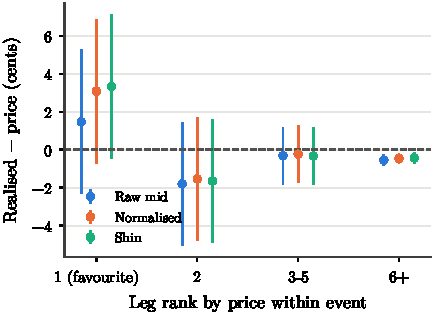
\includegraphics[width=0.55\textwidth]{figures/fig_xs_multi.pdf}
\caption{Multi-outcome events (mutually exclusive, at least three legs): realised frequency minus
price, in cents, by the leg's price rank within its event, for the raw mid, the mid normalised to
sum to one, and the Shin probability $\hat p_k(\shinz)$. 95\% confidence intervals clustered by
event.}\label{fig:xs-multi}
\end{figure}

\clearpage

\section{Additional results: trade-level flow}\label{app:flow}
\subsection{Sample design and coverage}\label{app:flow-design}

\Cref{tab:flow-design} lists the strata of the trade sample. The design weight of an event is
its stratum's frame-to-sample event ratio, times $L_e/20$ when the event has $L_e>20$ traded
legs. Sports leagues are identified from the series ticker. ``Other sports'' collects the
remaining leagues, including motor racing, minor soccer and basketball leagues, table tennis
and the Ballon d'Or.

\begin{table}[htbp]
\centering
\begin{threeparttable}
\caption{Sampling frame and stratified sample of the trade-level analysis}\label{tab:flow-design}
\small
\begin{tabular}{lrrrrr}
\toprule
 & \multicolumn{2}{c}{Frame} & \multicolumn{2}{c}{Sample} & \\
\cmidrule(lr){2-3}\cmidrule(lr){4-5}
Stratum & Events & Markets & Events & Markets & Weight per event \\
\midrule
% source: data/research/flb_flow/sample_plan.json
%BEGIN:design
% source: data/research/flb_flow (generated by flb_flow tex)
Combat & 1,295 & 4,688 & 60 & 208 & 21.6 \\
Cricket & 1,154 & 3,463 & 60 & 213 & 19.2 \\
Esports & 32,301 & 67,181 & 150 & 306 & 215.3 \\
Golf & 779 & 12,229 & 40 & 231 & 19.5 \\
MLB & 22,948 & 231,556 & 100 & 624 & 229.5 \\
NBA & 3,935 & 61,082 & 50 & 609 & 78.7 \\
NCAAF & 11,871 & 126,743 & 80 & 891 & 148.4 \\
NFL & 7,995 & 99,542 & 60 & 491 & 133.2 \\
NHL & 4,621 & 44,803 & 60 & 375 & 77.0 \\
Other sports & 43,694 & 147,595 & 150 & 475 & 291.3 \\
Soccer & 32,087 & 134,290 & 120 & 473 & 267.4 \\
Tennis & 30,489 & 65,940 & 150 & 318 & 203.3 \\
WNBA & 2,646 & 19,812 & 60 & 488 & 44.1 \\
Entertainment & 1,160 & 12,095 & 260 & 2,492 & 4.5 \\
Mentions & 349 & 7,230 & 120 & 2,048 & 2.9 \\
Politics & 801 & 4,589 & 260 & 1,515 & 3.1 \\
Science \& Tech & 426 & 3,200 & 220 & 1,615 & 1.9 \\
Weather & 12,303 & 82,218 & 300 & 1,957 & 41.0 \\
%END:design
\bottomrule
\end{tabular}
\begin{tablenotes}\footnotesize
\item Frame: settled, non-financial Kalshi markets that closed 15~August--31~October 2026 and
traded at least once. Events are drawn uniformly at random within each stratum (seed
20261111). Weight per event: frame events divided by sample events.
\end{tablenotes}
\end{threeparttable}
\end{table}

\begin{table}[htbp]
\centering
\begin{threeparttable}
\caption{Coverage of the main trade sample by group}\label{tab:flow-coverage}
\footnotesize
\setlength{\tabcolsep}{4pt}
\begin{tabular}{@{}lrrrrrrrr@{}}
\toprule
 & & & & Taker & Contracts & Taker \$ & Dropped & Complete \\
Group & Markets & Events & Prints & orders & (m) & (m) & (\%) & (\%) \\
\midrule
% source: data/research/flb_flow/summary.json (coverage)
%BEGIN:coverage
% source: data/research/flb_flow (generated by flb_flow tex)
Sports & 5,026 & 1,003 & 1,529,207 & 994,330 & 191.84 & 92.30 & 40.9 & 100 \\
Weather & 1,720 & 297 & 203,699 & 96,491 & 4.03 & 1.79 & 17.7 & 100 \\
Politics & 1,489 & 258 & 339,908 & 213,216 & 37.93 & 17.81 & 10.2 & 100 \\
Entertainment & 2,435 & 258 & 278,713 & 161,512 & 22.48 & 10.10 & 9.4 & 100 \\
Mentions & 1,921 & 119 & 245,400 & 126,128 & 9.21 & 3.07 & 43.5 & 100 \\
Science \& Tech & 1,573 & 216 & 88,190 & 51,857 & 11.19 & 6.59 & 3.3 & 100 \\
%END:coverage
\bottomrule
\end{tabular}
\begin{tablenotes}\footnotesize
\item Counts after the pre-resolution filter. Taker \$ is the taker side's notional,
$\sum n\q$. Dropped: the share of all fetched prints removed by the filter. Complete: the median
across markets of contracts printed over the market's reported volume.
\end{tablenotes}
\end{threeparttable}
\end{table}

\subsection{Choosing the pre-resolution cut}\label{app:flow-preres}

% source: data/research/flb_flow/summary.json (pre_resolution)
\Cref{tab:flow-preres} motivates the cut-offs. In sports the share of contracts traded at
$\le3\cents$ or $\ge97\cents$ is 3--10\% more than half an hour before the close. It then rises
to about 20\% at 10--30 minutes, about 35\% at 5--10 minutes and 65--75\% in the last five
minutes. These are games that are already decided and sweeps after the final whistle. In
non-sports markets that closed early, the share jumps from 22--35\% to 72--89\% in the last hour,
while the event that closed the market unfolds. The four-hour cut is deliberately wider than
that, because the moment the event occurred is not observed. In markets that closed on schedule,
extreme prices are common at every horizon. They come from the far legs of multi-outcome events,
which are genuine longshots, so they are kept.

\begin{table}[htbp]
\centering
\begin{threeparttable}
\caption{Share of contracts traded at extreme prices by minutes before the close (\%)}\label{tab:flow-preres}
\footnotesize
\begin{tabular}{@{}lrrrrr@{}}
\toprule
 & \multicolumn{2}{c}{Sports} & \multicolumn{2}{c}{Non-sports} & Share of \\
\cmidrule(lr){2-3}\cmidrule(lr){4-5}
Minutes before close & On schedule & Early & On schedule & Early & volume \\
\midrule
% source: data/research/flb_flow/summary.json (pre_resolution)
%BEGIN:preres
% source: data/research/flb_flow (generated by flb_flow tex)
0--5 & $75$ & $65$ & $61$ & $89$ & 5.2 \\
5--10 & $35$ & $34$ & $68$ & $86$ & 4.8 \\
10--30 & $22$ & $18$ & $54$ & $80$ & 15.6 \\
30--60 & $9$ & $10$ & $62$ & $72$ & 15.0 \\
60--240 & $4$ & $3$ & $67$ & $22$ & 32.5 \\
$>240$ & $5$ & $8$ & $45$ & $35$ & 26.8 \\
%END:preres
\bottomrule
\end{tabular}
\begin{tablenotes}\footnotesize
\item All fetched prints of the main sample, before any filter. Extreme: YES price $\le3\cents$
or $\ge97\cents$; contract-weighted, unweighted by design. Closed early: closed more than 30
minutes before the scheduled expiration. Share of volume: the window's share of all contracts.
\end{tablenotes}
\end{threeparttable}
\end{table}

\subsection{Returns by price bucket}\label{app:flow-buckets}

\Cref{tab:flow-buckets} and \cref{fig:flow-roles-groups} give pooled, design-weighted returns by
price bucket for both roles, overall and by group. \Cref{tab:flow-yesno} splits takers by the
side they bought. The pooled longshot cells are dominated by a few upsets
(\cref{sec:res-flow-roles}); the per-stratum medians in the main text are the robust summary.

\begin{figure}[htbp]
\centering
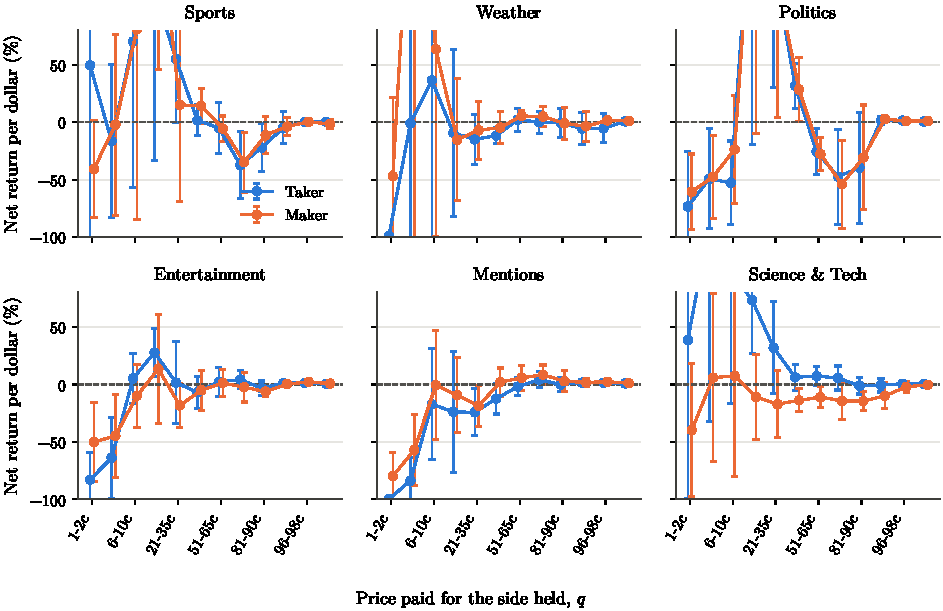
\includegraphics[width=\textwidth]{figures/fig_flow_roles_groups.pdf}
\caption{Takers against makers by price bucket and group. Net return per dollar
(dollar-weighted, after each role's fee) of taker and maker positions, by the price of the side
held, with 95\% confidence intervals clustered by event. Main sample, design-weighted.}\label{fig:flow-roles-groups}
% source: data/research/flb_flow/tables/roles_bucket.csv
\end{figure}

\begin{table}[htbp]
\centering
\begin{threeparttable}
\caption{Taker and maker returns by the price of the side held}\label{tab:flow-buckets}
\footnotesize
\setlength{\tabcolsep}{4pt}
\begin{tabular}{@{}lrrrrr@{}}
\toprule
 & Taker & \multicolumn{2}{c}{Taker} & \multicolumn{2}{c}{Maker} \\
\cmidrule(lr){3-4}\cmidrule(lr){5-6}
Side price $\q$ & share (\%) & Gross (\cents) & Net (\%/\$) & Gross (\cents) & Net (\%/\$) \\
\midrule
% source: data/research/flb_flow/tables/roles_bucket.csv
%BEGIN:roles_bucket
% source: data/research/flb_flow (generated by flb_flow tex)
1--2\cents & $56$ & $+0.48$ $(0.4)$ & $+29.5$ $(0.3)$ & $-0.55$ $(-2.1)$ & $-41.9$ $(-2.2)$ \\
3--5\cents & $56$ & $-0.46$ $(-0.3)$ & $-17.2$ $(-0.5)$ & $+0.06$ $(0.0)$ & $+0.8$ $(0.0)$ \\
6--10\cents & $64$ & $+6.18$ $(1.2)$ & $+68.3$ $(1.1)$ & $+6.40$ $(1.0)$ & $+78.7$ $(1.0)$ \\
11--20\cents & $56$ & $+19.67$ $(1.5)$ & $+113.3$ $(1.5)$ & $+31.02$ $(2.4)$ & $+183.1$ $(2.6)$ \\
21--35\cents & $46$ & $+17.22$ $(2.2)$ & $+54.7$ $(2.0)$ & $+4.77$ $(0.4)$ & $+15.1$ $(0.4)$ \\
36--50\cents & $46$ & $+2.29$ $(0.7)$ & $+1.5$ $(0.2)$ & $+6.54$ $(1.9)$ & $+14.1$ $(1.8)$ \\
51--65\cents & $58$ & $-1.40$ $(-0.2)$ & $-5.0$ $(-0.5)$ & $-2.93$ $(-0.9)$ & $-5.5$ $(-1.0)$ \\
66--80\cents & $49$ & $-26.70$ $(-2.3)$ & $-37.2$ $(-2.5)$ & $-25.62$ $(-2.5)$ & $-34.7$ $(-2.6)$ \\
81--90\cents & $41$ & $-17.95$ $(-2.0)$ & $-21.9$ $(-2.0)$ & $-9.49$ $(-1.4)$ & $-11.2$ $(-1.4)$ \\
91--95\cents & $39$ & $-4.02$ $(-0.6)$ & $-4.8$ $(-0.7)$ & $-3.40$ $(-0.9)$ & $-3.7$ $(-0.9)$ \\
96--98\cents & $44$ & $+0.30$ $(0.3)$ & $+0.1$ $(0.1)$ & $+0.41$ $(0.4)$ & $+0.4$ $(0.3)$ \\
99\cents & $42$ & $+0.47$ $(2.5)$ & $+0.4$ $(2.1)$ & $-1.17$ $(-0.7)$ & $-1.2$ $(-0.7)$ \\
%END:roles_bucket
\bottomrule
\end{tabular}
\begin{tablenotes}\footnotesize
\item Main sample, all groups, design-weighted. Each print contributes a taker position at $\q$
and a maker position at $1-\q$, and both are sorted by the price of the side held. Taker share:
the takers' share of the contracts held at that price. Gross: contract-weighted
\eqref{eq:flow-c} with $\fee=0$, in cents. Net: dollar-weighted \eqref{eq:flow-d} after fees, in
percent. $t$-statistics clustered by event are in parentheses.
\end{tablenotes}
\end{threeparttable}
\end{table}

\begin{table}[htbp]
\centering
\begin{threeparttable}
\caption{YES-takers against NO-takers at equal side price}\label{tab:flow-yesno}
\footnotesize
\begin{tabular}{lrrrr}
\toprule
Taker price $\q$ & YES share (\%) & YES-taker, \%/\$ & NO-taker, \%/\$ & Difference \\
\midrule
% source: data/research/flb_flow/tables/yesno_cells.csv, yesno_diff.csv, yesno_share.csv
%BEGIN:yesno
% source: data/research/flb_flow (generated by flb_flow tex)
1--2\cents & $79$ & $+57.3$ $(0.5)$ & $-90.8$ $(-21.0)$ & $+148.1$ $(1.2)$ \\
3--5\cents & $85$ & $-14.2$ $(-0.4)$ & $-33.3$ $(-0.9)$ & $+19.0$ $(0.4)$ \\
6--10\cents & $85$ & $+67.0$ $(1.0)$ & $+75.3$ $(0.9)$ & $-8.3$ $(-0.1)$ \\
11--20\cents & $85$ & $+124.8$ $(1.5)$ & $+48.4$ $(1.0)$ & $+76.4$ $(0.8)$ \\
21--35\cents & $78$ & $+57.1$ $(1.8)$ & $+46.5$ $(2.5)$ & $+10.6$ $(0.4)$ \\
36--50\cents & $73$ & $-6.3$ $(-0.6)$ & $+23.2$ $(1.4)$ & $-29.5$ $(-1.3)$ \\
51--65\cents & $74$ & $-10.4$ $(-0.6)$ & $+11.2$ $(1.2)$ & $-21.6$ $(-1.0)$ \\
66--80\cents & $71$ & $-42.9$ $(-2.7)$ & $-22.9$ $(-1.8)$ & $-20.1$ $(-2.3)$ \\
81--90\cents & $62$ & $-31.7$ $(-2.5)$ & $-5.9$ $(-1.1)$ & $-25.8$ $(-3.2)$ \\
91--95\cents & $48$ & $-9.1$ $(-0.9)$ & $-0.7$ $(-0.2)$ & $-8.4$ $(-1.4)$ \\
96--98\cents & $45$ & $+0.1$ $(0.1)$ & $+0.1$ $(0.1)$ & $-0.0$ $(-0.0)$ \\
99\cents & $53$ & $+0.4$ $(1.7)$ & $+0.4$ $(1.3)$ & $+0.0$ $(0.1)$ \\
%END:yesno
\bottomrule
\end{tabular}
\begin{tablenotes}\footnotesize
\item Main sample, all groups, taker positions only, design-weighted. Net return per dollar is
dollar-weighted \eqref{eq:flow-d}, in percent. YES share: the share of taker contracts at that
price bought as YES. Difference: YES minus NO, in percentage points, with an event-clustered $t$
that accounts for shared events.
\end{tablenotes}
\end{threeparttable}
\end{table}

\subsection{Trade size by sector}\label{app:flow-size}

\Cref{tab:flow-size-sector} repeats \cref{tab:flow-size} separately for sports and non-sports
markets. The longshot share of small orders is twice as high outside sports.

\begin{table}[htbp]
\centering
\begin{threeparttable}
\caption{Taker flow and returns by order size, sports and non-sports}\label{tab:flow-size-sector}
\footnotesize
\setlength{\tabcolsep}{4pt}
\begin{tabular}{@{}llrrrrrr@{}}
\toprule
 & & \multicolumn{2}{c}{Share of taker} & Share at & Mean & \multicolumn{2}{c}{Taker net return per dollar} \\
\cmidrule(lr){3-4}\cmidrule(lr){7-8}
Sector & Order size & orders & contracts & $\q\le10\cents$ & $\q$ (\cents) & Longshots & Favourites \\
\midrule
% source: data/research/flb_flow/tables/size_shares_sector.csv, size_side_sector.csv
%BEGIN:size_sector
% source: data/research/flb_flow (generated by flb_flow tex)
Sports & $\le$\$10 & $51.7$ & $4.7$ & $36.3$ & $23$ & $+36.1$ $(0.8)$ & $-2.7$ $(-1.2)$ \\
 & \$10--100 & $37.7$ & $20.9$ & $17.0$ & $35$ & $+55.3$ $(1.1)$ & $-1.0$ $(-0.4)$ \\
 & \$100--1k & $9.5$ & $31.8$ & $8.3$ & $47$ & $+27.3$ $(0.6)$ & $-1.4$ $(-0.5)$ \\
 & $>$\$1k & $1.2$ & $42.7$ & $1.2$ & $58$ & $+169.0$ $(1.2)$ & $-3.8$ $(-1.0)$ \\
Non-sports & $\le$\$10 & $67.1$ & $20.7$ & $74.0$ & $13$ & $-35.2$ $(-1.3)$ & $-2.4$ $(-1.1)$ \\
 & \$10--100 & $24.8$ & $32.3$ & $46.4$ & $30$ & $-23.1$ $(-1.0)$ & $-3.4$ $(-1.1)$ \\
 & \$100--1k & $7.0$ & $27.7$ & $21.6$ & $56$ & $-29.7$ $(-1.3)$ & $-0.9$ $(-0.6)$ \\
 & $>$\$1k & $1.1$ & $19.4$ & $2.6$ & $81$ & $-85.1$ $(-4.6)$ & $+0.5$ $(0.6)$ \\
%END:size_sector
\bottomrule
\end{tabular}
\begin{tablenotes}\footnotesize
\item As \cref{tab:flow-size}, separately for sports and non-sports markets. Shares are in
percent within the sector. Returns are dollar-weighted \eqref{eq:flow-d} after the taker fee,
with event-clustered $t$-statistics in parentheses.
\end{tablenotes}
\end{threeparttable}
\end{table}

\subsection{Timing cells}\label{app:flow-timing}

\Cref{tab:flow-timing-cells} lists taker flow and returns in every timing and attention cell
used in \cref{sec:res-flow-timing}.

\begin{table}[htbp]
\centering
\begin{threeparttable}
\caption{Taker flow and returns by timing and attention cell}\label{tab:flow-timing-cells}
\footnotesize
\begin{tabular}{@{}lrrrrr@{}}
\toprule
 & Volume & \multicolumn{2}{c}{Taker return per dollar (\%)} & Share at & Orders \\
\cmidrule(lr){3-4}
Cell & share (\%) & Net & Gross & $\q\le10\cents$ (\%) & $\le\$100$ (\%) \\
\midrule
% source: data/research/flb_flow/tables/timing.csv
%BEGIN:timing_cells
% source: data/research/flb_flow (generated by flb_flow tex)
\multicolumn{6}{@{}l}{\emph{Hour of day (ET)}} \\
\quad 00--06 & $8.1$ & $-10.3$ $(-1.7)$ & $-8.2$ $(-1.4)$ & $11.2$ & $89.5$ \\
\quad 06--12 & $11.8$ & $-11.0$ $(-2.3)$ & $-8.9$ $(-1.8)$ & $9.5$ & $89.5$ \\
\quad 12--18 & $41.2$ & $-1.2$ $(-0.2)$ & $+1.3$ $(0.2)$ & $8.8$ & $88.8$ \\
\quad 18--24 & $38.8$ & $+0.9$ $(0.3)$ & $+3.4$ $(1.1)$ & $8.2$ & $89.9$ \\
\multicolumn{6}{@{}l}{\emph{Day}} \\
\quad Weekday & $72.6$ & $+0.7$ $(0.2)$ & $+3.2$ $(0.9)$ & $8.4$ & $89.5$ \\
\quad Weekend & $27.4$ & $-10.2$ $(-2.3)$ & $-8.1$ $(-1.8)$ & $10.0$ & $89.2$ \\
\multicolumn{6}{@{}l}{\emph{Sports game phase}} \\
\quad Pre-game & $33.4$ & $-3.4$ $(-0.4)$ & $-0.9$ $(-0.1)$ & $5.3$ & $91.6$ \\
\quad In play & $66.6$ & $-2.6$ $(-1.1)$ & $-0.3$ $(-0.1)$ & $8.5$ & $88.1$ \\
\multicolumn{6}{@{}l}{\emph{Sports game start}} \\
\quad Before 19:00 ET & $55.0$ & $-2.7$ $(-0.4)$ & $-0.4$ $(-0.1)$ & $8.7$ & $88.3$ \\
\quad 19:00--23:59 ET & $45.0$ & $-3.1$ $(-1.2)$ & $-0.7$ $(-0.3)$ & $6.0$ & $90.6$ \\
\multicolumn{6}{@{}l}{\emph{Time to scheduled expiry}} \\
\quad $<1$ h & $13.4$ & $-5.2$ $(-2.4)$ & $-3.2$ $(-1.4)$ & $9.7$ & $87.4$ \\
\quad 1--6 h & $70.2$ & $-0.4$ $(-0.1)$ & $+2.1$ $(0.6)$ & $7.5$ & $88.1$ \\
\quad 6--24 h & $10.7$ & $-1.5$ $(-0.1)$ & $+1.1$ $(0.1)$ & $9.2$ & $92.8$ \\
\quad 1--7 days & $4.5$ & $-26.8$ $(-2.2)$ & $-25.2$ $(-2.0)$ & $17.3$ & $96.1$ \\
\quad $>7$ days & $1.3$ & $-1.1$ $(-0.4)$ & $+0.9$ $(0.3)$ & $43.9$ & $90.1$ \\
\multicolumn{6}{@{}l}{\emph{Market age}} \\
\quad First 24 h & $23.0$ & $-5.8$ $(-1.6)$ & $-3.7$ $(-1.0)$ & $10.7$ & $86.3$ \\
\quad Later & $77.0$ & $-1.4$ $(-0.3)$ & $+1.1$ $(0.3)$ & $8.3$ & $90.2$ \\
\multicolumn{6}{@{}l}{\emph{Past-hour volume vs own average}} \\
\quad $<0.5\times$ & $2.7$ & $-13.8$ $(-2.0)$ & $-11.7$ $(-1.7)$ & $27.2$ & $92.0$ \\
\quad $0.5$--$3\times$ & $4.1$ & $-12.4$ $(-1.1)$ & $-10.5$ $(-0.9)$ & $16.0$ & $93.9$ \\
\quad $3$--$10\times$ & $7.2$ & $-12.2$ $(-1.4)$ & $-10.2$ $(-1.1)$ & $11.5$ & $93.3$ \\
\quad $\ge10\times$ & $86.0$ & $-0.7$ $(-0.2)$ & $+1.8$ $(0.5)$ & $6.9$ & $88.4$ \\
\multicolumn{6}{@{}l}{\emph{Event volume}} \\
\quad Below top decile & $14.1$ & $-3.3$ $(-1.2)$ & $-1.1$ $(-0.4)$ & $12.4$ & $89.3$ \\
\quad Top decile (marquee) & $85.9$ & $-2.3$ $(-0.6)$ & $+0.2$ $(0.0)$ & $8.3$ & $89.4$ \\
%END:timing_cells
\bottomrule
\end{tabular}
\begin{tablenotes}\footnotesize
\item Main sample, all groups, taker positions, design-weighted. Volume share: the cell's share
of taker contracts within the panel. Returns are dollar-weighted \eqref{eq:flow-d}, with
event-clustered $t$-statistics in parentheses. Share at $\q\le10\cents$: the share of taker
contracts bought at a longshot price. Orders $\le\$100$: the share of taker orders with a
notional of at most \$100. Game phase and start time cover sports games with a known scheduled
start. The past-hour volume ratio needs six hours of trading history.
\end{tablenotes}
\end{threeparttable}
\end{table}

\section{Additional results: wallets and venues}\label{app:wallets}
% Wallets workstream: appendix. Code: src/albert/research/flb_wallets.py
\subsection{Data access and robots.txt record}\label{app:wallets-robots}
% source: data/research/flb_wallets/summary.json:robots_txt
Following the project's data policy, we use a host only if its own \texttt{robots.txt} allows
our access. We checked each host on 11~November 2026.
\begingroup\sloppy
\begin{itemize}
  \item \url{data-api.polymarket.com} (trades, account statistics, price histories) and
    \url{gamma-api.polymarket.com} (markets, events, tags, resolutions) serve no
    \texttt{robots.txt}: the request returns HTTP 410 or 404, which places no restriction. Both are
    used, at no more than three requests per second.
  \item \url{polymarket.com} allows all agents (\texttt{User-agent: * / Disallow:}) and points AI
    agents to an \texttt{llms.txt}. We fetched nothing from it.
  \item \url{docs.polymarket.com} and \url{docs.polymarket.us} allow all agents
    (\texttt{Content-Signal: ai-input=yes}). We read their fee pages.
  \item \url{gateway.polymarket.us}, the Polymarket US data host, disallows \texttt{anthropic-ai},
    \texttt{ClaudeBot} and \texttt{Claude-Web}. We therefore use no Polymarket US market data. The
    venue enters the comparison only through its published fee schedule.
\end{itemize}
\endgroup
No order was placed on any venue, and no geoblocking workaround was used. Polymarket's
international exchange is used purely as a public data source.

\subsection{Fee schedules}\label{app:wallets-fees}
\Cref{tab:wallets-fees} lists the taker fee per contract on each venue at several side prices. All
three venues charge $\theta\,\q(1-\q)$ per contract, so the fee is largest in dollars at
50\cents{} and largest relative to the price for longshots: at $\q=5\cents$ a positive taker fee of
0.19--0.45\cents{} is 4--9\% of the price.
% source: data/research/flb_wallets/fees.csv; summary.json:coverage.fee_enabled_share_by_month (fee roll-out)
\begin{itemize}
  \item Polymarket International charges no maker fees. Its taker rate depends on the category
    (0.05 for sports, culture, weather and other; 0.04 for politics, mentions and tech; zero for
    geopolitics). Fees were switched on for almost every market in March--April 2026. Before that,
    almost all trading was fee-free.
  \item Polymarket US sets $\theta$ by the account's trailing 30-day taker volume, from 0.095
    below \$10{,}000 to 0.0695 above \$250{,}000 (effective 28~October 2026). Small accounts
    therefore pay the highest rate on any of the three venues.
\end{itemize}
\begin{table}[t]
\centering
\begin{threeparttable}
\caption{Taker fee per contract by venue (cents)}\label{tab:wallets-fees}
% source: data/research/flb_wallets/fees.csv (fee_table in flb_wallets.py; schedules checked 2026-11-11)
\begin{tabular}{rcccccc}
\toprule
& Kalshi & \multicolumn{3}{c}{Polymarket International} & \multicolumn{2}{c}{Polymarket US} \\
\cmidrule(lr){3-5}\cmidrule(lr){6-7}
$\q$ (\cents) & & Sports & Politics & Geopolitics & $<\$10$k & $\geq\$250$k \\
\midrule
2 & 0.14 & 0.10 & 0.08 & 0 & 0.19 & 0.14 \\
5 & 0.33 & 0.24 & 0.19 & 0 & 0.45 & 0.33 \\
10 & 0.63 & 0.45 & 0.36 & 0 & 0.85 & 0.63 \\
25 & 1.31 & 0.94 & 0.75 & 0 & 1.78 & 1.30 \\
50 & 1.75 & 1.25 & 1.00 & 0 & 2.38 & 1.74 \\
\bottomrule
\end{tabular}
\begin{tablenotes}\footnotesize
\item Exact fee $\theta\,\q(1-\q)$ per contract before rounding. Kalshi: $\theta=0.07$; it computes
  fees per fill to \$0.000001, rebates rounding over-payment, and charges makers $0.0175\,\q(1-\q)$ on some series. Polymarket
  International (\url{docs.polymarket.com/trading/fees}): makers pay nothing; fees are in force
  from March--April 2026. Polymarket US (\url{docs.polymarket.us/fees}): the two columns are
  its lowest and highest volume tiers, with banker's rounding to the cent per order. Schedules
  checked on 11~November 2026.
\end{tablenotes}
\end{threeparttable}
\end{table}

\subsection{Sample, coverage and data checks}\label{app:wallets-coverage}
% source: data/research/flb_wallets/summary.json:coverage, summary.json:concentration.zero_sum_check
\Cref{tab:wallets-coverage} lists the frame and the trade sample by group and volume tier. The sample design
balances the groups. Sports make up 72.5\% of the frame's markets, but each group
contributes several hundred sampled markets, so group-level estimates are comparably precise and pooled
estimates are re-weighted with the design weights. Two checks support the trade data:
\begin{itemize}
  \item \emph{Exposure balance.} In 97.8\% of the 2{,}197 fee-free
    markets the YES-equivalent exposures of all wallets sum to zero, and in 99.95\%
    their PnL sums to zero within $10^{-6}$ of turnover, as \eqref{eq:wallets-pnl} requires when every fill is
    observed. In the 568 fee-charging markets the figure is
    85.9\%, because the taker's buy size there is net of the fee taken in
    shares. The total PnL of all wallets is within 1\% of turnover in 100\%
    of them.
  \item \emph{Resolution agreement.} For the cross-venue sample, Kalshi and Polymarket settle every matched
    team-side the same way (100\%).
\end{itemize}
Polymarket's taker fees cover 14\% of frame markets resolving in March 2026,
85\% in April and 100\% from May; earlier markets are fee-free.
0 sampled markets exceeded the 150-page cap and are excluded from the trade analyses.

\begin{table}[t]
\centering
\small
\begin{threeparttable}
\caption{Polymarket frame and trade sample}\label{tab:wallets-coverage}
% source: data/research/flb_wallets/summary.json:coverage (by_group, by_tier)
\begin{tabular}{lrrrr}
\toprule
& \multicolumn{2}{c}{Frame} & \multicolumn{2}{c}{Trade sample} \\
\cmidrule(lr){2-3}\cmidrule(lr){4-5}
& Markets & Volume (\$M) & Markets & Fills \\
\midrule
Sports & 461{,}685 & 51{,}677 & 481 & 295{,}004 \\
Weather & 115{,}966 & 1{,}099 & 362 & 360{,}575 \\
Politics & 29{,}382 & 19{,}858 & 480 & 508{,}491 \\
Entertainment & 14{,}526 & 2{,}060 & 466 & 478{,}494 \\
Mentions & 10{,}948 & 315 & 398 & 224{,}015 \\
Science \& Tech & 3{,}524 & 431 & 315 & 515{,}981 \\
Other & 489 & 400 & 263 & 191{,}915 \\
\midrule
\$1k-10k & 383{,}120 & & 1{,}126 & 185{,}467 \\
\$10k-100k & 183{,}614 & & 1{,}222 & 787{,}395 \\
\$100k-1M & 59{,}808 & & 386 & 1{,}232{,}656 \\
\$1M-6M & 8{,}638 & & 31 & 368{,}957 \\
\$>\$\$6M & 1{,}340 & & -- & -- \\
\bottomrule
\end{tabular}
\begin{tablenotes}\footnotesize
\item Frame: resolved Polymarket markets with $\geq\$1{,}000$ volume in events ending January 2024 to October
  2026, excluding financial tags. Sample: markets whose complete trade history was downloaded (maker and
  taker rows). Volume tiers by market volume; $>\$6$M markets are not sampled.
\end{tablenotes}
\end{threeparttable}
\end{table}

\subsection{Robustness of the class results}\label{app:wallets-robust}
\Cref{tab:wallets-robust} moves each class cut-off in turn. \Cref{tab:wallets-halves} splits the class results by
half of the sample. \Cref{tab:wallets-sizeage} replaces the classes with fill size, account age and
leaderboard status. \Cref{tab:wallets-holdexit} reports the hold-or-exit decomposition by class.

\begin{table}[t]
\centering
\small
\begin{threeparttable}
\caption{Robustness of the class results to the cut-offs}\label{tab:wallets-robust}
% source: data/research/flb_wallets/who_variants.csv
\setlength{\tabcolsep}{4pt}
\begin{tabular}{lrrrrrrrrrr}
\toprule
& \multicolumn{2}{c}{Retail} & \multicolumn{2}{c}{Active retail} & \multicolumn{2}{c}{Mid} & \multicolumn{2}{c}{Whale} & \multicolumn{2}{c}{MM} \\
\cmidrule(lr){2-3}\cmidrule(lr){4-5}\cmidrule(lr){6-7}\cmidrule(lr){8-9}\cmidrule(lr){10-11}
Variant & LS\$ & $\ret_{\LS}$ & LS\$ & $\ret_{\LS}$ & LS\$ & $\ret_{\LS}$ & LS\$ & $\ret_{\LS}$ & LS\$ & $\ret_{\LS}$ \\
\midrule
Baseline & 1.3 & $-$37 & 0.7 & $-$59 & 0.3 & $-$89 & 0.1 & $-$100 & 0.7 & $-$42 \\
Small $\leq\$50$ & 1.6 & $-$26 & 0.8 & $-$57 & 0.3 & $-$89 & 0.1 & $-$100 & 0.7 & $-$42 \\
Small $\leq\$250$ & 1.1 & $-$45 & 0.5 & $-$60 & 0.4 & $-$97 & 0.1 & $-$100 & 0.7 & $-$42 \\
Whale $\geq\$500$ & 1.3 & $-$37 & 0.7 & $-$59 & 0.4 & $-$89 & 0.1 & $-$99 & 0.7 & $-$42 \\
Whale $\geq\$5{,}000$ & 1.3 & $-$37 & 0.7 & $-$59 & 0.2 & $-$91 & 0.1 & $-$100 & 0.7 & $-$42 \\
Active: $\geq10$ fills & 1.6 & $-$36 & 0.7 & $-$56 & 0.3 & $-$89 & 0.1 & $-$100 & 0.7 & $-$42 \\
Active: $\geq50$ fills & 1.1 & $-$42 & 0.6 & $-$59 & 0.3 & $-$89 & 0.1 & $-$100 & 0.7 & $-$42 \\
MM loose (10, 0.5, 0.3) & 1.3 & $-$37 & 0.5 & $-$58 & 0.3 & $-$90 & 0.1 & $-$100 & 0.7 & $-$48 \\
MM strict (50, 0.9, 0.7) & 1.3 & $-$37 & 0.7 & $-$60 & 0.3 & $-$89 & 0.1 & $-$100 & 0.7 & $-$2 \\
\bottomrule
\end{tabular}
\begin{tablenotes}\footnotesize
\item LS\$: longshot share of dollars bought (\%); $\ret_{\LS}$: net return per dollar of longshot buys (\%),
  both dollar-weighted, buy fills before $t^{\mathrm{info}}$. Each row moves one cut-off of the baseline
  (small \$100, whale \$1{,}000, active 20 earlier fills, MM: 20 fills, maker share 0.7, two-sided share 0.5).
\end{tablenotes}
\end{threeparttable}
\end{table}

\begin{table}[t]
\centering
\small
\begin{threeparttable}
\caption{Class results by half of the sample}\label{tab:wallets-halves}
% source: data/research/flb_wallets/who_share.csv (dim=cls, half=H1/H2), ls_flow.csv (role=all, half=H1/H2)
\begin{tabular}{lrrrrrrrr}
\toprule
& \multicolumn{4}{c}{H1: January 2024 -- May 2025} & \multicolumn{4}{c}{H2: June 2025 -- October 2026} \\
\cmidrule(lr){2-5}\cmidrule(lr){6-9}
& LS fills & $\ret_{\LS}$ & \multicolumn{2}{c}{Net LS flow} & LS fills & $\ret_{\LS}$ & \multicolumn{2}{c}{Net LS flow} \\
\midrule
Retail & 15.2 & $-$89 & 1.67 & (2.4) & 11.1 & $-$18 & 0.29 & (3.3) \\
Active retail & 17.2 & $-$90 & 0.80 & (0.8) & 15.6 & $-$39 & $-$0.03 & ($-$0.5) \\
Mid & 5.3 & $-$96 & $-$0.10 & ($-$0.2) & 1.2 & $-$84 & $-$0.06 & ($-$1.1) \\
Whale & 2.1 & $-$100 & $-$0.30 & ($-$0.9) & 0.1 & $-$100 & $-$0.04 & ($-$1.6) \\
MM & 38.0 & $-$87 & $-$1.17 & ($-$1.5) & 20.0 & $-$9 & $-$0.04 & ($-$0.8) \\
\bottomrule
\end{tabular}
\begin{tablenotes}\footnotesize
\item LS fills: longshot share of design-weighted buy fills (\%); $\ret_{\LS}$: net return per dollar of longshot buys
  (\%, dollar-weighted); net LS flow: net longshot dollars bought per dollar traded (\%, $t$ in parentheses).
  Buy and sell fills before $t^{\mathrm{info}}$; $t$-statistics clustered by event.
\end{tablenotes}
\end{threeparttable}
\end{table}

\begin{table}[t]
\centering
\small
\begin{threeparttable}
\caption{Longshot buying by fill size, account age and leaderboard status}\label{tab:wallets-sizeage}
% source: data/research/flb_wallets/who_share.csv (half=All; dims size_bucket, age_bucket, lb)
\begin{tabular}{lrrrrrrrr}
\toprule
& & & \multicolumn{3}{c}{Longshot share (\%)} & FAV & \multicolumn{2}{c}{Longshot $\ret$} \\
\cmidrule(lr){4-6}\cmidrule(lr){8-9}
& Wallets & Fills & fills & \$ & ($t$) & \$ (\%) & \% & ($t$) \\
\midrule
\multicolumn{9}{l}{\emph{Fill size}} \\
\quad $\leq$\$10 & 133{,}995 & 828{,}526 & 23.1 & 7.6 & (6.0) & 14.8 & $-$22.2 & ($-$0.6) \\
\quad \$10--100 & 67{,}035 & 383{,}136 & 2.4 & 1.9 & (4.6) & 22.9 & $-$48.4 & ($-$2.4) \\
\quad \$100--1k & 20{,}785 & 97{,}225 & 0.7 & 0.6 & (2.4) & 15.4 & $-$77.6 & ($-$4.5) \\
\quad $>$\$1k & 3{,}278 & 10{,}420 & 0.2 & 0.1 & (1.6) & 7.9 & $-$100.0 & ($<-$100) \\
\multicolumn{9}{l}{\emph{Account age at the fill}} \\
\quad $<$7 days & 905 & 1{,}768 & 14.9 & 0.4 & (1.1) & 3.5 & $-$97.2 & ($-$40.2) \\
\quad 7--30 days & 1{,}031 & 3{,}540 & 8.3 & 0.2 & (1.4) & 9.1 & $-$88.3 & ($-$12.1) \\
\quad 30--180 days & 1{,}765 & 9{,}318 & 19.9 & 0.8 & (2.7) & 9.8 & 18.2 & (0.2) \\
\quad $>$180 days & 1{,}016 & 8{,}608 & 22.7 & 0.8 & (2.5) & 14.3 & $-$31.3 & ($-$0.5) \\
\multicolumn{9}{l}{\emph{All-time leaderboard (ex post)}} \\
\quad Leaderboard & 86 & 33{,}380 & 6.8 & 0.1 & (2.3) & 8.2 & $-$85.0 & ($-$11.3) \\
\quad Other & 188{,}115 & 1{,}285{,}927 & 15.4 & 0.6 & (3.2) & 11.9 & $-$52.6 & ($-$2.7) \\
\bottomrule
\end{tabular}
\begin{tablenotes}\footnotesize
\item Buy fills before $t^{\mathrm{info}}$. Account age uses the creation date of the address-selected wallet subset
  with account statistics. Shares and returns as in \cref{tab:wallets-class}; $t$-statistics clustered by event.
\end{tablenotes}
\end{threeparttable}
\end{table}

\begin{table}[t]
\centering
\small
\begin{threeparttable}
\caption{Holding to settlement versus exiting, by class and entry price}\label{tab:wallets-holdexit}
% source: data/research/flb_wallets/hold_exit.csv
\footnotesize
\setlength{\tabcolsep}{4pt}
\begin{tabular}{lrrcrrccrc}
\toprule
& \multicolumn{3}{c}{All positions} & \multicolumn{4}{c}{Longshot entries ($\q\le10\cents$)} & \multicolumn{2}{c}{\FAV{} entries} \\
\cmidrule(lr){2-4}\cmidrule(lr){5-8}\cmidrule(lr){9-10}
& Pos. & Exited & Exit VA & Pos. & Exited & Hold $\ret$ & Exit VA & Exited & Exit VA \\
& & \% & \% ($t$) & & \% & \% ($t$) & \% ($t$) & \% & \% ($t$) \\
\midrule
Retail & 262{,}487 & 21.4 & $-$3.3 ($-$1.1) & 43{,}801 & 41.7 & $-$66.9 ($-$4.0) & 28.1 (1.8) & 28.2 & $-$0.5 ($-$2.1) \\
Active retail & 46{,}392 & 6.3 & 0.0 (0.1) & 9{,}693 & 6.9 & $-$91.8 ($-$21.6) & 4.4 (1.7) & 10.3 & $-$0.3 ($-$2.4) \\
Mid & 19{,}761 & 12.8 & $-$2.1 ($-$1.2) & 880 & 16.9 & $-$97.1 ($-$64.0) & 19.1 (2.6) & 27.4 & $-$0.6 ($-$3.0) \\
Whale & 1{,}885 & 21.3 & $-$4.9 ($-$1.9) & 33 & 0.5 & $-$99.0 ($-$81.4) & $-$0.1 ($-$0.1) & 55.5 & $-$8.8 ($-$1.4) \\
MM & 43{,}662 & 18.6 & 2.4 (1.9) & 13{,}153 & 54.7 & $-$77.4 ($-$6.8) & 51.5 (3.0) & 23.6 & $-$1.1 ($-$2.5) \\
\addlinespace
All & 374{,}187 & 16.1 & $-$1.4 ($-$1.3) & 67{,}560 & 28.9 & $-$81.6 ($-$10.6) & 23.2 (2.2) & 24.4 & $-$1.2 ($-$2.1) \\
\bottomrule
\end{tabular}
\begin{tablenotes}\footnotesize
\item Positions: wallet $\times$ market $\times$ outcome, opened by a buy before $t^{\mathrm{info}}$. Exited: share (\%, cost-
  and design-weighted) with at least half of the shares sold before the close. Exit VA: realised minus
  hold-to-settlement PnL per dollar of cost (\%). Hold $\ret$: return per dollar if every share were held.
  Gross of fees; $t$-statistics clustered by event.
\end{tablenotes}
\end{threeparttable}
\end{table}

\section{Additional results: structural decomposition}\label{app:structural}
% Workstream structural: supplementary tables and figures, generated by
% `python -m albert.research.flb_structural run latex` and paper_flb/scripts/fig_structural.py from
% data/research/flb_structural/ (band_cells.csv, band_tick_grid.csv, weighting_*.csv, shin_*.csv,
% beliefs_coef.csv, decomposition.csv, summary.json).

This appendix supports \cref{sec:res-structural}. The CSV files under \texttt{data/research/flb\_structural/} also
hold every bucket $\times$ lead $\times$ group cell of the band, the fits for each group and lead, and the $\shinz$ of
every event-lead.
\begin{itemize}
  \item \emph{Band.} \Cref{tab:structural-band-groups} splits the band decomposition by price bucket and group.
  \Cref{tab:structural-band-robust} varies:
  \begin{itemize}
    \item the cost of capital;
    \item the weights;
    \item the sample half;
    \item the quote age and the spread;
    \item the tick grid and the contract structure.
  \end{itemize}
  It also drops the five events with the largest absolute contribution to the residual.
  \item \emph{Weighting.} \Cref{tab:structural-weighting-cells,fig:structural-weighting} give the weighting
  functions by lead, structure and group.
  \item \emph{Shin.} \Cref{tab:structural-shin-full,tab:structural-shin-forecasts,fig:structural-shin} give
  $\shinz$ by lead, group and structure, and compare forecasts.
  \item \emph{Belief dispersion.} \Cref{tab:structural-beliefs,tab:structural-beliefs-groups,fig:structural-beliefs}
  report the slope interactions, pooled, by group and by half.
  \item \emph{Synthesis.} \Cref{tab:structural-scorecard} lists every prediction tested and
  \cref{tab:structural-decomp} the counterfactual shares.
\end{itemize}

% BEGIN AUTO:tab-band-groups
\begin{table}[!htbp]
\centering
\begin{threeparttable}
\caption{The band by group and longshot bucket}\label{tab:structural-band-groups}
\scriptsize
\setlength{\tabcolsep}{3pt}
\begin{tabular}{@{}lrrrrrrrrrrr@{}}
\toprule
 & & & & Gross & \multicolumn{4}{c}{Band components} & Residual & Maker & In band \\
\cmidrule(lr){6-9}
Cell & Sides & Events & $\bar\q$ & $\bar\q-\bar\won$ & Floor & Half-spr. & Fee & Capital & $\bar R$ & $\bar R^{mk}$ & (\%) \\
\midrule
% source: data/research/flb_structural/band_cells.csv
\multicolumn{12}{@{}l}{\emph{All groups}} \\
\quad 1--2\cents & 26{,}184 & 2{,}118 & 0.87 & 0.49 (6.9) & 0.30 & 0.48 & 0.01 & 0.03 & $-$0.33 ($-$4.6) & 1.24 (16.9) & 100 \\
\quad 3--5\cents & 9{,}521 & 2{,}007 & 3.53 & 1.86 (9.0) & 0.00 & 2.40 & 0.08 & 0.04 & $-$0.65 ($-$3.2) & 4.21 (19.4) & 100 \\
\quad 6--10\cents & 4{,}847 & 1{,}707 & 7.53 & 2.01 (4.1) & 0.00 & 2.22 & 0.34 & 0.04 & $-$0.60 ($-$1.2) & 4.18 (8.4) & 100 \\
\multicolumn{12}{@{}l}{\emph{Sports}} \\
\quad 1--2\cents & 6{,}211 & 303 & 0.79 & 0.46 (3.1) & 0.35 & 0.39 & 0.00 & 0.05 & $-$0.32 ($-$2.2) & 1.14 (7.4) & 100 \\
\quad 3--5\cents & 1{,}914 & 280 & 3.56 & 2.25 (5.8) & 0.00 & 2.67 & 0.06 & 0.04 & $-$0.52 ($-$1.4) & 4.85 (11.3) & 100 \\
\quad 6--10\cents & 983 & 276 & 7.63 & 2.02 (1.7) & 0.00 & 2.21 & 0.32 & 0.03 & $-$0.54 ($-$0.5) & 4.16 (3.4) & 100 \\
\multicolumn{12}{@{}l}{\emph{Weather}} \\
\quad 1--2\cents & 2{,}126 & 317 & 0.97 & 0.24 (0.7) & 0.27 & 0.56 & 0.01 & 0.03 & $-$0.63 ($-$1.9) & 1.04 (3.2) & 100 \\
\quad 3--5\cents & 1{,}122 & 455 & 3.68 & 1.57 (2.6) & 0.00 & 2.38 & 0.09 & 0.02 & $-$0.92 ($-$1.5) & 3.94 (6.4) & 100 \\
\quad 6--10\cents & 657 & 384 & 7.52 & 3.29 (3.4) & 0.00 & 2.33 & 0.34 & 0.02 & 0.59 (0.6) & 5.60 (5.8) & 82 \\
\multicolumn{12}{@{}l}{\emph{Politics}} \\
\quad 1--2\cents & 7{,}720 & 728 & 0.93 & 0.41 (2.7) & 0.25 & 0.56 & 0.01 & 0.03 & $-$0.44 ($-$2.9) & 1.19 (7.9) & 100 \\
\quad 3--5\cents & 2{,}597 & 563 & 3.49 & 0.66 (1.2) & 0.00 & 2.14 & 0.09 & 0.05 & $-$1.62 ($-$3.0) & 2.76 (5.1) & 100 \\
\quad 6--10\cents & 1{,}451 & 482 & 7.54 & 0.70 (0.7) & 0.00 & 2.17 & 0.35 & 0.06 & $-$1.89 ($-$1.9) & 2.81 (2.8) & 100 \\
\multicolumn{12}{@{}l}{\emph{Entertainment}} \\
\quad 1--2\cents & 6{,}011 & 377 & 0.90 & 0.66 (6.1) & 0.29 & 0.54 & 0.00 & 0.02 & $-$0.20 ($-$1.9) & 1.47 (12.3) & 100 \\
\quad 3--5\cents & 2{,}169 & 353 & 3.48 & 2.77 (10.2) & 0.00 & 2.76 & 0.05 & 0.04 & $-$0.09 ($-$0.3) & 5.49 (18.6) & 100 \\
\quad 6--10\cents & 759 & 266 & 7.39 & 1.74 (1.3) & 0.00 & 2.33 & 0.33 & 0.07 & $-$0.99 ($-$0.7) & 4.01 (2.9) & 100 \\
\multicolumn{12}{@{}l}{\emph{Mentions}} \\
\quad 1--2\cents & 982 & 58 & 0.72 & 0.72 (24.0) & 0.39 & 0.18 & 0.01 & 0.02 & 0.12 (5.9) & 1.27 (25.0) & 83 \\
\quad 3--5\cents & 423 & 64 & 3.60 & 2.57 (5.7) & 0.00 & 1.53 & 0.14 & 0.02 & 0.88 (2.0) & 4.08 (7.5) & 66 \\
\quad 6--10\cents & 513 & 82 & 7.65 & 2.38 (1.6) & 0.00 & 2.02 & 0.37 & 0.02 & $-$0.03 (0.0) & 4.38 (2.9) & 100 \\
\multicolumn{12}{@{}l}{\emph{Science \& Tech}} \\
\quad 1--2\cents & 2{,}967 & 311 & 0.87 & 0.48 (2.4) & 0.30 & 0.47 & 0.01 & 0.03 & $-$0.33 ($-$1.6) & 1.21 (5.8) & 100 \\
\quad 3--5\cents & 1{,}184 & 267 & 3.38 & 1.93 (3.2) & 0.00 & 2.13 & 0.09 & 0.06 & $-$0.35 ($-$0.6) & 3.97 (6.4) & 100 \\
\quad 6--10\cents & 421 & 189 & 7.37 & 2.48 (1.7) & 0.00 & 2.24 & 0.34 & 0.09 & $-$0.19 ($-$0.1) & 4.60 (3.1) & 100 \\
\bottomrule
\end{tabular}
\begin{tablenotes}\footnotesize
\item As \cref{tab:structural-band}, by group and price bucket, leads pooled, $\rho=5\%$, market-weighted. $t$-statistics clustered by event in parentheses.
\end{tablenotes}
\end{threeparttable}
\end{table}
% END AUTO:tab-band-groups

% BEGIN AUTO:tab-band-robust
\begin{table}[!htbp]
\centering
\begin{threeparttable}
\caption{The band: cost of capital, weights, halves and the tick grid}\label{tab:structural-band-robust}
\scriptsize
\setlength{\tabcolsep}{2.5pt}
\begin{tabular}{@{}lrrrrrrrrrrr@{}}
\toprule
 & & & & Gross & \multicolumn{4}{c}{Band components} & Residual & Maker & In band \\
\cmidrule(lr){6-9}
Cell & Sides & Events & $\bar\q$ & $\bar\q-\bar\won$ & Floor & Half-spr. & Fee & Capital & $\bar R$ & $\bar R^{mk}$ & (\%) \\
\midrule
% source: data/research/flb_structural/band_cells.csv, summary.json:band.robustness, band_tick_grid.csv
Main & 40{,}552 & 3{,}091 & 2.54 & 1.07 (10.0) & 0.18 & 1.23 & 0.07 & 0.04 & $-$0.45 ($-$4.3) & 2.44 (21.3) & 100 \\
$\rho=0$ & 40{,}552 & 3{,}091 & 2.54 & 1.07 (10.0) & 0.18 & 1.23 & 0.07 & 0.00 & $-$0.42 ($-$3.9) & 2.47 (21.6) & 100 \\
$\rho=10\%$ & 40{,}552 & 3{,}091 & 2.54 & 1.07 (10.0) & 0.18 & 1.23 & 0.07 & 0.07 & $-$0.49 ($-$4.6) & 2.40 (20.9) & 100 \\
Volume-weighted & 40{,}552 & 3{,}091 & 2.18 & 1.56 (5.1) & 0.27 & 0.39 & 0.10 & 0.02 & 0.79 (2.7) & 2.19 (7.3) & 50 \\
First half (to 2025-07) & 22{,}146 & 1{,}762 & 2.67 & 0.81 (5.1) & 0.17 & 1.30 & 0.08 & 0.03 & $-$0.76 ($-$4.8) & 2.24 (13.3) & 100 \\
Second half & 18{,}406 & 1{,}341 & 2.69 & 0.97 (5.4) & 0.18 & 1.19 & 0.08 & 0.04 & $-$0.52 ($-$2.9) & 2.29 (12.2) & 100 \\
Drop 5 influential events & 40{,}507 & 3{,}086 & 2.54 & 1.16 (11.7) & 0.18 & 1.23 & 0.07 & 0.04 & $-$0.36 ($-$3.7) & 2.53 (23.6) & 100 \\
Quote age $\le$ 24 h & 33{,}432 & 3{,}055 & 2.72 & 1.11 (9.2) & 0.16 & 1.29 & 0.08 & 0.04 & $-$0.46 ($-$3.9) & 2.52 (19.7) & 100 \\
Spread $\le$ 5\cents & 35{,}751 & 2{,}868 & 2.11 & 0.80 (7.4) & 0.21 & 0.80 & 0.07 & 0.04 & $-$0.31 ($-$2.9) & 1.77 (16.0) & 100 \\
Pinned at the floor & 15{,}801 & 1{,}445 & 0.50 & 0.37 (7.5) & 0.50 & 0.00 & 0.00 & 0.03 & $-$0.16 ($-$3.3) & 0.83 (16.9) & 100 \\
Above the floor & 24{,}751 & 2{,}889 & 3.67 & 1.46 (9.1) & 0.00 & 1.91 & 0.11 & 0.04 & $-$0.61 ($-$3.8) & 3.33 (20.1) & 100 \\
With a bid ($\q^b>0$) & 12{,}404 & 2{,}494 & 4.98 & 1.42 (5.3) & 0.00 & 1.68 & 0.22 & 0.04 & $-$0.52 ($-$1.9) & 3.05 (11.3) & 100 \\
Binary & 8{,}484 & 1{,}324 & 3.26 & 1.58 (6.5) & 0.12 & 1.47 & 0.11 & 0.03 & $-$0.14 ($-$0.6) & 3.14 (12.4) & 100 \\
Multi-outcome & 10{,}045 & 291 & 1.69 & 1.04 (7.3) & 0.27 & 0.89 & 0.03 & 0.04 & $-$0.20 ($-$1.5) & 2.16 (12.1) & 100 \\
Ladder leg & 13{,}819 & 884 & 2.87 & 0.84 (3.9) & 0.13 & 1.42 & 0.09 & 0.03 & $-$0.83 ($-$3.9) & 2.35 (10.6) & 100 \\
Deadline & 8{,}204 & 608 & 2.10 & 0.90 (4.1) & 0.22 & 1.01 & 0.06 & 0.07 & $-$0.46 ($-$2.1) & 2.06 (8.9) & 100 \\
1\cents{} grid, 1--2\cents & 25{,}800 & 2{,}093 & 0.87 & 0.49 (6.8) & 0.30 & 0.48 & 0.01 & 0.03 & $-$0.34 ($-$4.7) & 1.24 (16.7) & 100 \\
0.1\cents{} grid, 1--2\cents & 384 & 31 & 0.75 & 0.75 (10.2) & 0.01 & 0.50 & 0.02 & 0.05 & 0.17 (2.3) & 1.20 (8.7) & 77 \\
1\cents{} grid, all \LS & 39{,}960 & 3{,}061 & 2.55 & 1.07 (9.9) & 0.18 & 1.23 & 0.07 & 0.04 & $-$0.45 ($-$4.3) & 2.44 (21.2) & 100 \\
0.1\cents{} grid, all \LS & 592 & 36 & 1.94 & 0.92 (1.3) & 0.00 & 1.01 & 0.06 & 0.07 & $-$0.24 ($-$0.3) & 1.87 (2.5) & 100 \\
\bottomrule
\end{tabular}
\begin{tablenotes}\footnotesize
\item Longshot sides ($\q\le10\cents$ at the mid), leads pooled; columns as in \cref{tab:structural-band}. Halves split at the month that divides the quotes most evenly. The influential events are the five with the largest absolute contribution to the residual. Grid: markets quoted on Kalshi's 0.1\cents{} price grid against the standard 1\cents{} grid; the floor is one tick on each grid. $t$-statistics clustered by event in parentheses.
\end{tablenotes}
\end{threeparttable}
\end{table}
% END AUTO:tab-band-robust

\begin{figure}[!htbp]
\centering
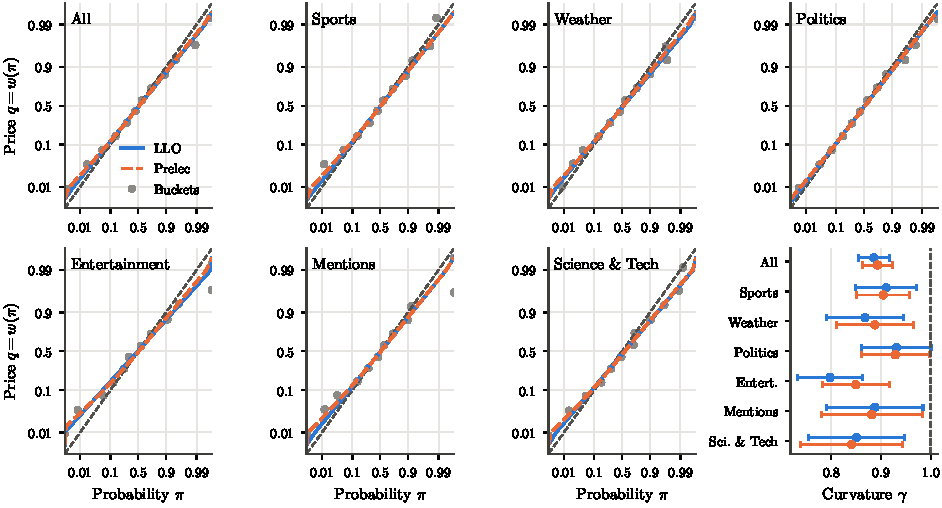
\includegraphics[width=\textwidth]{figures/fig_structural_weighting.pdf}
\caption{Fitted probability-weighting functions $\q=w(\pi)$ on log-odds axes: linear in log odds (LLO) and Prelec,
pooled and by group, with the calibration points (realised frequency, mean YES price) of the price buckets.
Buckets with no or only winning outcomes sit at the edges. The dashed diagonal is calibration. Last panel:
curvature $\gamma$ by group with 95\% confidence intervals clustered by event (LLO upper, Prelec lower marker).
YES sides of pre-event quotes, market-weighted.}\label{fig:structural-weighting}
\end{figure}

% BEGIN AUTO:tab-weighting-cells
\begin{table}[!htbp]
\centering
\begin{threeparttable}
\caption{Weighting-function parameters by lead and structure}\label{tab:structural-weighting-cells}
\scriptsize
\setlength{\tabcolsep}{3pt}
\begin{tabular}{@{}lrrrrrrrr@{}}
\toprule
 & & & \multicolumn{4}{c}{LLO} & \multicolumn{2}{c}{Prelec} \\
\cmidrule(lr){4-7}\cmidrule(l){8-9}
Cell & Quotes & Events & $\alpha$ & $\beta$ ($t_{\beta=1}$) & $\gamma$ & $\delta$ & $\gamma$ & $\delta$ \\
\midrule
% source: data/research/flb_structural/weighting_fits.csv
\multicolumn{9}{@{}l}{\emph{By lead}} \\
\quad 1h & 15{,}784 & 4{,}191 & 0.06 & 1.18 (7.1) & 0.85 (0.018) & $-$0.05 (0.033) & 0.87 (0.018) & 1.00 (0.018) \\
\quad 6h & 15{,}827 & 4{,}163 & 0.07 & 1.20 (7.7) & 0.84 (0.018) & $-$0.06 (0.032) & 0.85 (0.017) & 1.00 (0.017) \\
\quad 24h & 11{,}688 & 2{,}739 & 0.13 & 1.23 (7.8) & 0.81 (0.020) & $-$0.11 (0.040) & 0.83 (0.020) & 1.03 (0.022) \\
\quad 3d & 10{,}358 & 2{,}380 & 0.03 & 1.17 (5.9) & 0.86 (0.021) & $-$0.02 (0.045) & 0.89 (0.022) & 0.99 (0.024) \\
\quad 7d & 5{,}553 & 1{,}478 & $-$0.12 & 1.16 (3.8) & 0.86 (0.031) & 0.10 (0.069) & 0.91 (0.033) & 0.92 (0.036) \\
\quad 30d & 2{,}782 & 885 & $-$0.32 & 1.12 (2.3) & 0.89 (0.043) & 0.28 (0.087) & 0.98 (0.048) & 0.83 (0.041) \\
\multicolumn{9}{@{}l}{\emph{By structure}} \\
\quad Binary & 17{,}163 & 2{,}644 & $-$0.04 & 1.12 (3.7) & 0.89 (0.026) & 0.04 (0.038) & 0.91 (0.023) & 0.96 (0.022) \\
\quad Multi-outcome & 12{,}822 & 474 & 0.14 & 1.28 (4.4) & 0.78 (0.039) & $-$0.11 (0.037) & 0.84 (0.032) & 1.01 (0.013) \\
\quad Ladder leg & 22{,}392 & 1{,}030 & 0.14 & 1.12 (2.9) & 0.89 (0.032) & $-$0.13 (0.062) & 0.89 (0.033) & 1.05 (0.033) \\
\quad Deadline & 9{,}615 & 644 & 0.47 & 1.22 (3.9) & 0.82 (0.039) & $-$0.38 (0.108) & 0.77 (0.041) & 1.21 (0.067) \\
\multicolumn{9}{@{}l}{\emph{By group, volume-weighted}} \\
\quad All groups & 46{,}505 & 4{,}430 & $-$0.01 & 1.48 (3.6) & 0.68 (0.061) & 0.01 (0.130) & 0.76 (0.064) & 0.96 (0.082) \\
\quad Sports & 11{,}242 & 1{,}298 & $-$0.29 & 1.37 (2.0) & 0.73 (0.098) & 0.21 (0.119) & 0.86 (0.089) & 0.83 (0.067) \\
\quad Weather & 5{,}616 & 1{,}007 & $-$0.10 & 1.29 (2.0) & 0.77 (0.089) & 0.07 (0.133) & 0.86 (0.079) & 0.92 (0.068) \\
\quad Politics & 12{,}490 & 941 & 1.13 & 1.80 (6.6) & 0.56 (0.038) & $-$0.63 (0.305) & 0.53 (0.063) & 1.39 (0.228) \\
\quad Entertainment & 7{,}609 & 506 & 0.76 & 1.34 (3.0) & 0.74 (0.064) & $-$0.57 (0.249) & 0.68 (0.060) & 1.34 (0.164) \\
\quad Mentions & 4{,}517 & 102 & 0.07 & 1.35 (4.6) & 0.74 (0.041) & $-$0.05 (0.116) & 0.77 (0.044) & 0.99 (0.064) \\
\quad Science \& Tech & 4{,}678 & 503 & $-$0.13 & 1.56 (4.0) & 0.64 (0.058) & 0.08 (0.170) & 0.73 (0.058) & 0.92 (0.092) \\
\quad Other & 353 & 73 & 0.34 & 1.43 (1.5) & 0.70 (0.144) & $-$0.24 (0.361) & 0.71 (0.134) & 1.11 (0.230) \\
\bottomrule
\end{tabular}
\begin{tablenotes}\footnotesize
\item As \cref{tab:structural-weighting}. Within a lead each market counts once. Standard errors (or $t$) clustered by event in parentheses.
\end{tablenotes}
\end{threeparttable}
\end{table}
% END AUTO:tab-weighting-cells

\begin{figure}[!htbp]
\centering
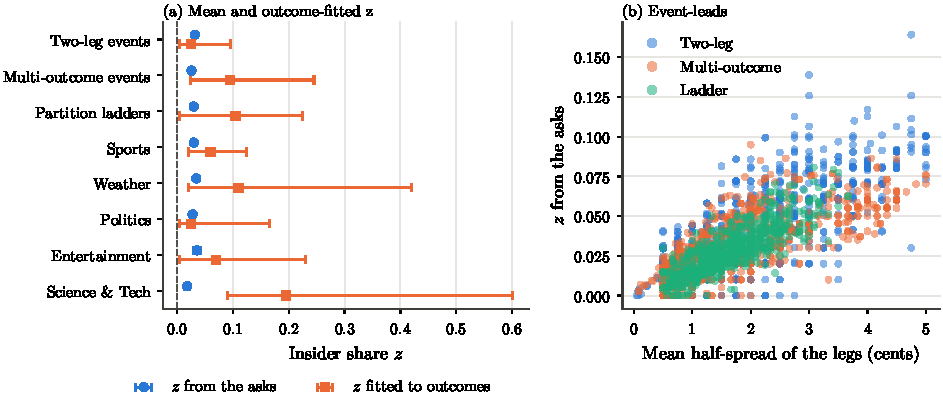
\includegraphics[width=\textwidth]{figures/fig_structural_shin.pdf}
\caption{Shin's insider share in partition events. Left: mean $\shinz$ implied by the asks (95\% confidence
intervals clustered by event) and $\shinz$ fitted to outcomes (95\% event-bootstrap intervals; the grid ends at
0.6), by structure and group. Right: $\shinz$ implied by the asks against the mean half-spread of the event's
legs, one point per event and lead.}\label{fig:structural-shin}
\end{figure}

% BEGIN AUTO:tab-shin-full
\begin{table}[!htbp]
\centering
\begin{threeparttable}
\caption{Shin's insider share by lead, group and structure}\label{tab:structural-shin-full}
\scriptsize
\setlength{\tabcolsep}{2.8pt}
\begin{tabular}{@{}lrrrrrrrr@{}}
\toprule
 & Event- & & Legs & $\sum a-1$ & $\sum p-1$ & $\shinz$ from & $\shinz$ from & $\shinz$ fitted \\
Sample & leads & Events & (med.) & (\%) & (\%) & asks & mids & to outcomes [95\% CI] \\
\midrule
% source: data/research/flb_structural/shin_cells.csv
\multicolumn{9}{@{}l}{\emph{By lead}} \\
\quad 1h & 1{,}143 & 1{,}143 & 2 & 6.9 (24.9) & 1.2 (9.1) & 0.031 (0.0008) & 0.004 & 0.060 [0.025, 0.135] \\
\quad 6h & 1{,}187 & 1{,}187 & 2 & 7.4 (23.2) & 1.2 (7.5) & 0.030 (0.0007) & 0.005 & 0.135 [0.075, 0.225] \\
\quad 24h & 729 & 729 & 3 & 8.4 (20.7) & 1.4 (8.2) & 0.030 (0.0008) & 0.004 & 0.115 [0.065, 0.185] \\
\quad 3d & 559 & 559 & 3 & 10.6 (18.3) & 1.9 (8.8) & 0.027 (0.0009) & 0.004 & 0.010 [0.000, 0.095] \\
\quad 7d & 242 & 242 & 2 & 8.1 (9.4) & 1.6 (3.9) & 0.030 (0.0013) & 0.005 & 0.010 [0.000, 0.080] \\
\quad 30d & 95 & 95 & 2 & 10.1 (6.9) & 1.8 (2.5) & 0.038 (0.0032) & 0.007 & 0.020 [0.000, 0.600] \\
\multicolumn{9}{@{}l}{\emph{By group and structure}} \\
\quad Sports, two-leg & 1{,}609 & 660 & 2 & 3.1 (38.3) & $-$0.2 ($-$4.2) & 0.032 (0.0008) & 0.003 & 0.020 [0.000, 0.095] \\
\quad Sports, multi & 764 & 256 & 3 & 9.0 (12.4) & 1.4 (4.1) & 0.026 (0.0010) & 0.003 & 0.155 [0.035, 0.530] \\
\quad Weather, partition ladder & 237 & 139 & 6 & 15.5 (25.5) & 4.1 (11.4) & 0.034 (0.0014) & 0.010 & 0.110 [0.020, 0.420] \\
\quad Politics, two-leg & 376 & 74 & 2 & 2.5 (13.9) & 0.0 (0.0) & 0.031 (0.0020) & 0.003 & 0.050 [0.015, 0.370] \\
\quad Politics, multi & 217 & 46 & 6 & 11.5 (11.8) & 3.2 (7.5) & 0.030 (0.0024) & 0.008 & 0.020 [0.005, 0.331] \\
\quad Politics, partition ladder & 418 & 160 & 9 & 17.7 (29.4) & 3.7 (11.8) & 0.026 (0.0009) & 0.006 & 0.100 [0.000, 0.265] \\
\quad Entertainment, two-leg & 24 & 6 & 2 & 4.3 (4.8) & 0.5 (2.0) & 0.057 (0.0132) & 0.006 & 0.600 [0.600, 0.600] \\
\quad Entertainment, multi & 94 & 35 & 10 & 19.6 (8.4) & 6.9 (6.0) & 0.032 (0.0031) & 0.010 & 0.035 [0.000, 0.220] \\
\quad Science \& Tech, multi & 214 & 44 & 7 & 7.6 (5.4) & 1.8 (2.3) & 0.018 (0.0019) & 0.005 & 0.195 [0.090, 0.600] \\
\bottomrule
\end{tabular}
\begin{tablenotes}\footnotesize
\item As \cref{tab:structural-shin}. Regression of $\shinz$ from the asks on the mean half-spread, log legs and group dummies (Sports omitted), weighted, event-clustered $t$ in parentheses: half-spread (\cents) 0.0168 (50.5); log legs $-$0.0037 ($-$5.8); Weather 0.0029 (2.7); Politics 0.0039 (4.7); Entertainment 0.0114 (5.7); Science \& Tech 0.0059 (4.2); $R^2=0.68$, 3{,}955 event-leads.
\end{tablenotes}
\end{threeparttable}
\end{table}
% END AUTO:tab-shin-full

% BEGIN AUTO:tab-shin-forecasts
\begin{table}[!htbp]
\centering
\begin{threeparttable}
\caption{Partition events: raw, normalised and Shin probabilities}\label{tab:structural-shin-forecasts}
\footnotesize
\setlength{\tabcolsep}{3.5pt}
\begin{tabular}{@{}lrrrrl@{}}
\toprule
 & \multicolumn{2}{c}{Longshot legs (\cents)} & \multicolumn{3}{c}{Log score gain (milli-nats)} \\
\cmidrule(lr){2-3}\cmidrule(l){4-6}
Forecast & All months & Second half & All months & Second half & against \\
\midrule
% source: data/research/flb_structural/summary.json:shin.longshot_legs, shin_scores.csv
Raw mid & 0.93 (4.9) & 1.08 (4.3) & -- & -- & -- \\
Normalised mids & 0.83 (4.4) & 1.01 (4.1) & $-$0.41 ($-$3.2) & $-$0.69 ($-$3.6) & raw mid \\
Normalised asks & -- & -- & -- & -- & -- \\
Shin, from the asks & 0.94 (5.0) & 1.06 (4.3) & 3.47 (8.5) & 3.47 (6.2) & normalised asks \\
Shin, from the mids & -- & -- & 0.86 (5.0) & 0.89 (3.3) & normalised mids \\
Shin, $\shinz$ fitted on the first half & $-$0.21 ($-$1.1) & 0.05 (0.2) & 1.45 (1.7) & 1.79 (1.5) & normalised mids \\
\bottomrule
\end{tabular}
\begin{tablenotes}\footnotesize
\item Legs of the partition events of \cref{tab:structural-shin}. Longshot legs: mid at most 10\cents{} (8{,}906 legs in all months, 3{,}747 in the second half); mean forecast minus outcome in cents. Log score: mean gain per leg, over all legs, against the normalisation of the same prices. The fitted $\shinz$ is estimated on the first half of the months, so the second half is out of sample. Each event weighs one across its leads; $t$-statistics clustered by event in parentheses.
\end{tablenotes}
\end{threeparttable}
\end{table}
% END AUTO:tab-shin-forecasts

\begin{figure}[!htbp]
\centering
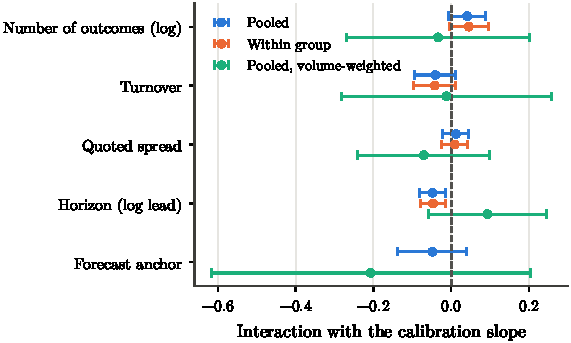
\includegraphics[width=0.66\textwidth]{figures/fig_structural_beliefs.pdf}
\caption{Interaction of each characteristic with the calibration slope, $b_k$ in~\eqref{eq:structural-interact}:
the change in the logit slope per standard deviation (per unit for the 0/1 anchor). Positive values mean a stronger
favourite--longshot bias. Pooled, within groups (group-specific slopes; the anchor is absorbed) and pooled
volume-weighted. 95\% confidence intervals clustered by event.}\label{fig:structural-beliefs}
\end{figure}

% BEGIN AUTO:tab-beliefs
\begin{table}[!htbp]
\centering
\begin{threeparttable}
\caption{Where is the bias steeper? Calibration-slope interactions}\label{tab:structural-beliefs}
\scriptsize
\setlength{\tabcolsep}{3.5pt}
\begin{tabular}{@{}lrrrrrr@{}}
\toprule
 & \multicolumn{4}{c}{Slope interaction (logit)} & \multicolumn{2}{c}{Longshot overpricing (\cents)} \\
\cmidrule(lr){2-5}\cmidrule(l){6-7}
 & Pooled & Within group & Volume-wtd. & Split anchor & Within group & Split anchor \\
\midrule
% source: data/research/flb_structural/beliefs_coef.csv
Number of outcomes (log) & 0.041 (1.7) & 0.045 (1.8) & $-$0.034 ($-$0.3) & 0.044 (1.8) & 0.01 (0.1) & $-$0.03 ($-$0.4) \\
Turnover & $-$0.041 ($-$1.5) & $-$0.043 ($-$1.5) & $-$0.013 ($-$0.1) & $-$0.042 ($-$1.6) & $-$0.06 ($-$0.6) & $-$0.01 ($-$0.2) \\
Quoted spread & 0.012 (0.7) & 0.009 (0.5) & $-$0.070 ($-$0.8) & 0.012 (0.7) & 0.57 (3.4) & 0.57 (3.4) \\
Horizon (log lead) & $-$0.048 ($-$2.8) & $-$0.047 ($-$2.8) & 0.093 (1.2) & $-$0.046 ($-$2.7) & $-$0.28 ($-$3.0) & $-$0.29 ($-$3.0) \\
Forecast anchor (0/1) & $-$0.049 ($-$1.1) &  & $-$0.207 ($-$1.0) &  &  &  \\
Anchor: Sports (0/1) &  &  &  & $-$0.065 ($-$1.3) &  & 0.12 (0.4) \\
Anchor: Weather (0/1) &  &  &  & $-$0.007 ($-$0.1) &  & $-$0.06 ($-$0.2) \\
\midrule
Events & 4{,}770 & 4{,}770 & 4{,}430 & 4{,}770 & 3{,}091 & 3{,}091 \\
Observations & 61{,}992 & 61{,}992 & 46{,}505 & 61{,}992 & 40{,}552 & 40{,}552 \\
\bottomrule
\end{tabular}
\begin{tablenotes}\footnotesize
\item Columns 1--4: coefficients $b_k$ of~\eqref{eq:structural-interact}, the change in the calibration slope per standard deviation of each characteristic (per unit for 0/1 anchors), YES sides of pre-event quotes; $b_k>0$ means a stronger bias. Pooled: one slope plus interactions, group intercepts; within group: group-specific slopes, so the group-level anchor is absorbed. Columns 5--6: least squares of the price minus outcome of longshot sides (cents per contract) on the standardised characteristics with price-bucket (and in column 5 group) fixed effects. Market-weighted unless stated; $t$-statistics clustered by event in parentheses.
\end{tablenotes}
\end{threeparttable}
\end{table}
% END AUTO:tab-beliefs

% BEGIN AUTO:tab-beliefs-groups
\begin{table}[!htbp]
\centering
\begin{threeparttable}
\caption{Calibration-slope interactions by group and by half}\label{tab:structural-beliefs-groups}
\scriptsize
\setlength{\tabcolsep}{3.5pt}
\begin{tabular}{@{}lrrrrrr@{}}
\toprule
Sample & Outcomes & Turnover & Spread & Horizon & Quotes & Events \\
\midrule
% source: data/research/flb_structural/beliefs_coef.csv, summary.json:beliefs
Sports & -- & 0.025 (0.6) & 0.019 (0.6) & $-$0.013 ($-$0.5) & 18{,}303 & 1{,}521 \\
Weather & -- & $-$0.054 ($-$0.4) & 0.043 (0.9) & 0.087 (1.9) & 6{,}796 & 1{,}065 \\
Politics & -- & $-$0.127 ($-$2.7) & 0.036 (1.2) & $-$0.080 ($-$2.0) & 15{,}774 & 968 \\
Entertainment & -- & $-$0.101 ($-$1.8) & 0.034 (0.6) & $-$0.203 ($-$3.8) & 10{,}424 & 530 \\
Mentions & -- & $-$0.107 ($-$1.7) & $-$0.064 ($-$1.1) & $-$0.059 ($-$1.2) & 4{,}743 & 103 \\
Science \& Tech & -- & $-$0.088 ($-$1.3) & $-$0.002 (0.0) & $-$0.099 ($-$1.4) & 5{,}472 & 510 \\
\midrule
Pooled, first half (to 2025-07) & 0.025 (0.9) & $-$0.067 ($-$2.0) & 0.036 (1.5) & $-$0.041 ($-$1.7) & 31{,}006 & 2{,}443 \\
\quad anchor & \multicolumn{4}{l}{0.096 (1.5)} & & \\
Pooled, second half & 0.049 (1.5) & $-$0.032 ($-$0.8) & $-$0.009 ($-$0.4) & $-$0.062 ($-$2.9) & 30{,}986 & 2{,}339 \\
\quad anchor & \multicolumn{4}{l}{$-$0.204 ($-$3.4)} & & \\
\bottomrule
\end{tabular}
\begin{tablenotes}\footnotesize
\item As \cref{tab:structural-beliefs}, column 1, estimated separately by group (a characteristic enters when at least ten events lie on each side of its group median) and by half of the sample. Positive interactions across groups: number of outcomes 0 of 0, turnover 1 of 6, quoted spread 4 of 6, horizon 1 of 6. $t$-statistics clustered by event in parentheses.
\end{tablenotes}
\end{threeparttable}
\end{table}
% END AUTO:tab-beliefs-groups

% BEGIN AUTO:tab-scorecard
\begin{table}[!htbp]
\centering
\begin{threeparttable}
\caption{The four explanations scored against their predictions}\label{tab:structural-scorecard}
\footnotesize
\setlength{\tabcolsep}{4pt}
\begin{tabular}{@{}p{0.6\textwidth}rr@{}}
\toprule
Prediction & Statistic & Holds \\
\midrule
% source: data/research/flb_structural/criteria.csv, summary.json:synthesis.criteria
\multicolumn{3}{@{}l}{\emph{H1: partly supported (2 of 5 predictions)}} \\
\quad Longshot mispricing inside the taker band ($\bar R$, \cents) & $-$0.45 ($-$4.3) & yes \\
\quad Inside the taker band, volume-weighted ($\bar R$, \cents) & 0.79 (2.7) & no \\
\quad Inside the taker band in every group (Bonferroni) & 6 of 6 & yes \\
\quad Gross mispricing rises with the lead (\cents{} per log hour) & $-$0.143 ($-$2.7) & no \\
\quad Concentrated at the tick floor (floor share $\ge0.5$) & 0.17 & no \\
\multicolumn{3}{@{}l}{\emph{H2: partly supported (4 of 5 predictions)}} \\
\quad Pooled $\gamma<1$ ($\gamma$, $t_{\gamma<1}$) & 0.89 (7.4) & yes \\
\quad $\gamma<1$ in every group (point estimates) & 6 of 6 & yes \\
\quad Equal $\gamma$ across groups not rejected (Wald $\chi^2$) & 8.6 ($p=0.127$) & yes \\
\quad LLO beats calibrated prices out of sample, both directions & 0.46, 0.04 (0.9, 0.1) & no \\
\quad Pooled LLO predicts as well as group-specific LLO & $-$3.10, $-$1.83 ($-$4.2, $-$3.1) & yes \\
\multicolumn{3}{@{}l}{\emph{H3: partly supported (2 of 4 predictions)}} \\
\quad Shin from the asks removes the longshot-leg overpricing (\cents) & 0.94 (5.0) & no \\
\quad $\shinz$ from the asks higher in information groups, given the spread & 0.004 (5.5) & yes \\
\quad Fitted $\shinz$ higher in information than in public groups & 0.015 [$-$0.110, 0.090] & no \\
\quad Longshot overpricing rises with $\shinz$ (\cents{} per unit) & 22.0 (2.1) & yes \\
\multicolumn{3}{@{}l}{\emph{H4: not supported (0 of 4 predictions)}} \\
\quad Steeper slope with more outcomes, within groups & 0.045 (1.8) & no \\
\quad Steeper slope with more turnover, within groups & $-$0.043 ($-$1.5) & no \\
\quad Flatter slope with a public forecast anchor & $-$0.049 ($-$1.1) & no \\
\quad Turnover interaction positive in most groups & 1 of 6 & no \\
\bottomrule
\end{tabular}
\begin{tablenotes}\footnotesize
\item Each row is a prediction of Hypotheses~\ref{hyp:mech}--\ref{hyp:beliefs} as made operational in \cref{sec:method-structural}, tested at the 5\% level; the every-group band test uses a one-sided Bonferroni threshold across groups. Statistics: cents per contract with $t$ (\cref{hyp:mech} band and horizon rows; the floor row is a share), $\gamma$ with $t_{\gamma<1}$, $\chi^2$ with $p$, out-of-sample log-score differences in milli-nats per quote for the two directions with $t$, cents per contract, $\shinz$ differences with 95\% bootstrap intervals, and slope interactions with $t$. All $t$-statistics and intervals clustered by event. Verdict: supported when every prediction holds, partly supported when some do.
\end{tablenotes}
\end{threeparttable}
\end{table}
% END AUTO:tab-scorecard

% BEGIN AUTO:tab-decomp
\begin{table}[!htbp]
\centering
\begin{threeparttable}
\caption{How much of the longshot loss does each explanation map remove?}\label{tab:structural-decomp}
\footnotesize
\setlength{\tabcolsep}{4pt}
\begin{tabular}{@{}lrrr@{}}
\toprule
Map from prices to probabilities & Removed (\cents) & Residual (\cents) & Share removed (\%) \\
\midrule
% source: data/research/flb_structural/decomposition.csv, summary.json:synthesis.counterfactual
\multicolumn{4}{@{}l}{\emph{Longshot sides, second half (18{,}406 sides, 1{,}341 events); gross mispricing 1.12 (6.9) \cents}} \\
\quad Taker band, $\rho=5\%$ (band 1.48\cents) & 1.12 & -- & 100 \\
\quad LLO, pooled, fitted on the first half & 0.69 & 0.43 (2.7) & 61 \\
\quad LLO by group, fitted on the first half & 0.92 & 0.20 (1.2) & 82 \\
\quad Prelec, pooled, fitted on the first half & 0.76 & 0.36 (2.3) & 68 \\
\multicolumn{4}{@{}l}{\emph{Longshot legs of partition events, second half (3{,}747 legs, 269 events); gross mispricing 1.08 \cents}} \\
\quad Normalised mids & 0.06 & 1.01 (4.1) & 6 \\
\quad Shin from the asks & 0.02 & 1.06 (4.3) & 2 \\
\quad Shin with $\shinz$ fitted on the first half & 1.02 & 0.05 (0.2) & 95 \\
\bottomrule
\end{tabular}
\begin{tablenotes}\footnotesize
\item Gross mispricing: price at the mid minus outcome, cents per contract. Band: the share of the gross mispricing that lies inside the taker band (\cref{tab:structural-band}). Each other row replaces the price by a fitted probability and reports the remaining price-minus-outcome gap (residual) and the share removed. The maps are alternative readings of the same calibration curve, not additive components. Market-weighted (partition events: each event once); $t$-statistics clustered by event in parentheses.
\end{tablenotes}
\end{threeparttable}
\end{table}
% END AUTO:tab-decomp


\end{document}
